\documentclass[12ptt,fleqn]{metrobk}

%TODO Zuerst ein paar Einstellungen vornehmen:
%Folgende Zeile aktiviert T1-Codierung (mit Postscript- oder ec/dc-Schriften)
\usepackage[T1]{fontenc}
\usepackage[utf8]{inputenc}

%TODO Zur Verwendung von Postscriptschriften:
\usepackage{lmodern}
%\usepackage{courierv}
%\usepackage{mathbeg}
\usepackage[dvips]{epsfig}
\usepackage{shortvrb}
\usepackage{array}

%TODO Alternativ können Sie babel verwenden:
%\usepackage{german}
\usepackage[german]{babel}
%\usepackage{apametro}

%TODO apametro/mharvard Zitationsstil
%\usepackage{metrocite}
\usepackage{mharvard}

%TODO MY PACKAGES
\usepackage{amsmath}
\usepackage{mathtools}
\usepackage{amssymb}
\usepackage{esint}
\usepackage{graphicx}
\usepackage{ziffer}
\usepackage{wrapfig}

%TODO BIRGITS PACKAGES
\usepackage{floatrow}
\usepackage{acronym}
\usepackage{tikz}
\usetikzlibrary{arrows,positioning}
\usepackage[normalem]{ulem}
\usepackage{psfrag}
\usepackage{enumerate}
\usepackage{pifont}
\usepackage{bibentry}
\usepackage{pstricks}
\usepackage{marvosym}
\usepackage{rotating}
\usepackage{paralist} 
\usepackage{enumitem}
\usepackage{color}
\usepackage{xcolor}
\usepackage{longtable}
\usepackage{verbatim}
\usepackage{fancybox}
\usepackage{paralist}
\usepackage{makeidx} 
\usepackage[intoc]{nomencl}
\usepackage[percent]{overpic}
\usepackage{enumitem}

%DISSERTATIONSINFORMATIONEN
\title{Endogenes Wachstum und Internationaler Handel}
%Your thesis title, this is used in the title and abstract
\subtitle{Die Wirkung von Außenhandelseffekten auf den technischen Fortschritt}
%Untertitle der Arbeit
\newcommand{\supname}{\emph{Prof. Dr. rer. pol. Susanne Soretz}}
%Your supervisor's name, print it elsewhere with \supname
\newcommand{\examname}{\emph{Prof. Dr. rer. pol. Armin Rohde}}
%Your examiner's name,print it elsewhere with \examname
\newcommand{\degree}{\emph{Doktor rerum politicarum}}
%Your degree name,print it elsewhere with \degreename
\author{Birgit Kirschbaum}
%Your name,print it elsewhere with \authorname
\newcommand{\addressname}{\emph{}}
%Your address,print it elsewhere with \addressname
\newcommand{\subject}{\emph{Bereich der Wirtschaftswissenschaften}}
%Your subject area,print it elsewhere with \subjectname
\newcommand{\univname}{\href{https://www.uni-greifswald.de/}{Erst-Moritz-Arndt Universität Greifswald}}
%Your university's name and URL,print it elsewhere with \univname
\newcommand{\deptname}{\href{https://rsf.uni-greifswald.de/en/lehrstuehle/wiwi/avwl/}{Allgemeine Volkswirtschaftslehre}}
%Your department's name and URL, print it elsewhere with \deptname
\newcommand{\groupname}{\href{https://rsf.uni-greifswald.de/en/lehrstuehle/wiwi/avwl/lehrstuhl-soretz/}{Lehrstuhl für AVWL sowie Wachstum, Strukturwandel und Handel}}
%Your research group's name and URL, print it elsewhere with \groupname
\newcommand{\facname}{\href{https://rsf.uni-greifswald.de/en/}{Rechts- und Staatswissenschaftliche Fakultät}}
%Your faculty's name and URL, print it elsewhere with \facname

%TODO Metropolis-Infos
\Reihe{Dissertation zur Erlangung des akademischen Grades eines \degree}
\Band{}
\ISBN{1-11111-111-1}
\Jahr{2016}
\Druck{Metropolis, Marburg}

%Einige häufige Trennfehler (bzw. unschöne Trennungen):
\hyphenation{eine einer eines weder wegen hatte alle aller lege legen
	quote Ihres Ihren Ihrem Ihre Times Wachs-tum Wachs-tums-rate
	Wachs-tums-raten Wirt-schafts-wachs-tum Wirt-schafts-wachs-tums
	docu-ment-class metro-art metro-bk Post-script Post-script-schrift
	Post-script-schrif-ten Dateien Klas-sen-dateien Mo-no-gra-phien 
	Sei-ten-um-bruch Sei-ten-um-brü-che}

\setcounter{tocdepth}{3}
\setcounter{secnumdepth}{3}
\begin{document}

\makefulltitle

%keine Kopf/Fußzeilen und Seitenummmern
\frontmatter
%TODO TOCTOCTOC FOR EVERYTHING
\tableofcontents % Prints the main table of contents
\listoffigures % Prints the list of figures
\listoftables % Prints the list of tables

%TODO INSERT ABBREVIATIONS
\chapter*{Abkürzungsverzeichnis}
\addcontentsline{toc}{chapter}{Abkürzungsverzeichnis}
\begin{acronym}[WTG] %statt WTG ->längester abkürzung damit einzug nach längster abkürzung ausgerichtet
	\acro{BIP}{Bruttoinlandsprodukt}
	\acro{bzw.}{beziehungsweise}
	\acro{FAO}{Food and Agriculture Organization of the United Nations}
	\acro{GG}{Gleichgewicht}
	\acro{GM}{General Motors Company}
	\acro{IWF}{Internationaler Währungsfonds}
	\acro{LTG}{lokale Technologiegrenze}
	\acro{UNO}{United Nations Organization}
	\acro{USA}{Vereinigte Staaten von Amerika}
	\acro{VW}{Volkswirtschaft}
	\acro{WTG}{Welttechnologiegrenze}
	\acro{WTO}{World Trade Organization} 
	\acro{z.B.}{zum Beispiel}
\end{acronym}

\mainmatter
% Include the chapters of the thesis as separate files from the content folder
% Uncomment the lines as you write the chapters
\chapter{Einleitung}\label{Einleitung}
%
Blickt man auf das vergangene Jahrtausend zurück, so haben nach \cite{Maddison.2001} drei einschneidende interaktive Ereignisse den Entwicklungsprozess der Welt bestimmt:\footnote{Dabei sind hier vor allem Ereignisse mit ökonomischer Wirkung von Bedeutung. Somit werden politische Begebenheiten und die damit zusammenhängenden wirtschaftlichen Konsequenzen vernachlässigt.}
%
\begin{itemize}
	\item Umsiedlung und Landerschließung
	\item Handel
	\item technischer Fortschritt
\end{itemize}
%
Das Augenmerk dieser Arbeit liegt vor allem auf den beiden zuletzt genannten Punkten: Handel und technischer Fortschritt. Beide Ereignisse dienen hier als Grundlage theoretischer Modellanalysen, bei denen zwei Wachstumsmodelle, basierend auf technischem Fortschritt, um den Aspekt des Außenhandels erweitert werden. Dabei wird zunächst die Humankapitalakkumulation und die damit einhergehende Erhöhung des Bildungsniveaus analysiert, bevor im Anschluss die Veränderung der Innovations- und Imitationstätigkeit von Volkswirtschaften durch die strategischen Entscheidungen von Unternehmen betrachtet wird. In diesem Zusammenhang wird die Wirkung außenwirtschaftlicher Effekte auf den technischen Fortschritt hervorgehoben. Es wird gezeigt, dass die Offenheit und somit der Außenhandel die technologische Entwicklung eines Landes fördert, was langfristig zu einem anhaltenden Wirtschaftswachstum führt. \\
%
Die Folgen und Konsequenzen der von \cite{Maddison.2001} genannten Ereignisse werden im Folgenden kurz beispielhaft erläutert, um die Notwendigkeit dieser wissenschaftlichen Arbeit zu unterstreichen. \cite[S. 17]{Maddison.2001} schildert, dass die Besiedelung und Bewirtschaftung unerschlossener Regionen zu einer Erweiterung des Faktors Boden führte. Als kurze Beispiele dienen China und die Erschließung des amerikanischen Kontinents.  In China ermöglichten neue Verfahren im Reisanbau eine Anpassung an die geologischen Rahmenbedingungen und eröffneten neue geographische Anbaumöglichkeiten. Nun konnte auch die Region südlich des Flusses Yangtse bewirtschaftet werden. Daraus folgte, dass sich vom achten~bis zum dreizehnten Jahrhundert Chinas Bevölkerung maßgeblich umsiedelte und sich damit an die neuen Bedingungen anpasste. Der prozentuale Bevölkerungsanteil hat sich südlich des Yangtse mehr als verdoppelt. Ähnlich verhielt es sich mit der Erschließung Amerikas durch die europäische Bevölkerung. Unbekanntes, fruchtbares Land sowie neue Ressourcen wurden entdeckt und eingesetzt, so dass die Produktivität anstieg und letztlich ein Einkommenszuwachs verursacht wurde \cite[S. 17-18]{Maddison.2001}.\\
%
Das zweite einschlägige Ereignis des letzten Jahrtausends war die Aufnahme von Handel zu anderen Staaten. Dies hat nach \cite{Maddison.2001} vor allem die europäischen Länder und weniger die afrikanischen und asiatischen Länder in ihrer Entwicklung  beeinflusst. Vom Jahr 1000 bis 1500 war bezüglich des internationalen, maritimen Handels Venedig von großer Bedeutung, nicht zuletzt aufgrund des Wissens um den Schiffbau und der strategische Lage. Es wurden überwiegend Seide und Gewürze mit fernöstlichen Ländern wie China und Syrien gehandelt. Schon damals bedingte die Offenheit eines Landes nicht nur die Einfuhr unbekannter Güter, sondern auch den Transfer von Produktionstechnologien und Wissen. Das westliche europäische Handelszentrum war Portugal. Ein weiterer Mitstreiter auf dem Gewürzhandelsmarkt waren die Niederlande, die jedoch erst ab 1500, eine ähnliche Flotte einsetzten. In den Niederlanden waren um 1700 nur 40{\%} der Erwerbsbevölkerung im landwirtschaftlichen Sektor beschäftigt. Der größte Teil des Volkseinkommens wurde durch die Seefahrt und den Dienstleistungssektor erwirtschaftet. Ähnlich verhielt es sich in Spanien, einer weiteren wichtigen maritimen Handelsmacht. Diese Zeit wurde geprägt durch starkes Konkurrenzdenken zu Lasten der Mitstreiter, denn Kooperationen wurden größtenteils vernachlässigt. Ebenfalls der Schifffahrt schlossen sich im 18. Jahrhundert Frankreich und England an. Englands Vorteil gegenüber seinen Mitstreitern lag in einem ausgebauten Netz an Institutionen im Banken- und Finanzsektor sowie staatlichen Einrichtungen. Das Wachstum Großbritanniens war zu dieser Zeit höher, als das aller anderen europäischen Länder. Unterstützend für die weltweiten Handelsrouten waren die Kolonien, die  die Erschließung von Ressourcen und Rohstoffen erlaubten und Grund für die Überwindung bisher ferner Distanzen lieferten \cite[S. 20]{Maddison.2001}.
Mit der Industrialisierung begann hinsichtlich des Wirtschaftswachstums ein neues Zeitalter. Bedingt durch den technischen Fortschritt wuchs das Pro-Kopf-Einkommen Großbritanniens schneller als jemals zuvor. Es gelang den Engländern ihren physischen Kapitalstock erheblich aufzubauen sowie die steigende Nachfrage nach qualifizierten Arbeitskräften durch den Ausbau des Bildungssystems zu befriedigen. Außerdem begann das britische Empire Handelsbeschränkungen zu reduzieren, was einen positiven Effekt auf die übrige Welt hatte, da dies auch den Diffusionsprozess von technischem Wissen begünstigte und somit die Industrialisierung in andere Länder trug. Auch die Einführung eines Eigentumsrechte-Systems des Staates steigerte die Attraktivität für Investoren.\footnote{Dieses Eigentumsrechte-System ist mit dem heutigen Patentrecht zu vergleichen.} England war ein wohlhabender Staat, der mit jeder Entwicklung die Welttechnologiegrenze ausweitete. \\
%
Die beiden Weltkriege zerstörten die Ordnung des freien Handels und das weltweite Wirtschaftswachstum war bis 1950 mehrheitlich deutlich geringer als bis zum Beginn des ersten Weltkrieges 1913. Die Nachkriegszeit nach dem zweiten Weltkrieg brachte vor allem in den europäischen Ländern eine Zeit des Aufschwungs mit sich. Das weltweite BIP stieg jährlich um etwa 5{\%} an, der weltweite Handel wuchs um 8{\%} und das Pro-Kopf-Einkommen um 3{\%} jährlich.\footnote{Diese Informationen basieren auf den Daten der OECD laut \cite{Maddison.2001}.} Die beiden Weltkriege brachten zudem eine neue politische Ordnung hervor. Der Kalte Krieg brach die Verbindung zwischen der westlichen Welt mit dem russisch wohl gesonnenen Osten ab. Internationaler Handel war trotz ausgebauter Transportmöglichkeiten eingeschränkter als Anfang des 20. Jahrhunderts \cite[S. 20-24]{Maddison.2001}.\\
%
Als dritten interaktiven Prozess nach \cite{Maddison.2001} wird erneut auf das letzte Jahrtausend zurückgeblickt, jedoch diesmal unter dem Aspekt der technologischen Entwicklung und der Einbettung von Institutionen. \\
%
Der technische Fortschritt war zwar von 1000-1820 verglichen mit heutigen Verhältnissen relativ gering, er war aber schon damals ein entscheidender Faktor für das Wirtschaftswachstum. Nur durch technische Errungenschaften der Seefahrt, wie beispielsweise dem Kompass, der Sanduhr und  weiterer Entwicklungen der Schifffahrt, gelang es, den Handel mit deutlich weiter entfernten Länder aufzunehmen. Außerdem konnten Neuerungen im landwirtschaftlichen Sektor das immer weiter ansteigende Bevölkerungswachstum kompensieren und ernsthafte Hungersnöte verhindern. Bis zum 15. Jahrhundert wurden viele technologische Neuerungen aus dem asiatischen und arabischen Raum nach Europa transferiert. Trotzdem profitierten letztendlich die europäischen Länder stärker als die Herkunftsländer selbst. Als einen der entscheidenden Unterschiede sieht \cite{Maddison.2001} die angesprochenen Institutionen wie das intakte Finanz-, Versicherungs- und Bankensystem, deren Vorreiter England war. Auch der Devisenmarkt erleichterte den Händlern der damaligen Zeit ihre Arbeit und minderte ihre Transaktionskosten erheblich. \\
%
Der Transfer dieses Systems oder neuer Technologien von Europa aus in die übrige Welt war jedoch relativ gering. Ein funktionierender Wirkungskanal des 18. Jahrhunderts waren die Kolonien Großbritanniens in Nordamerika \cite[S. 27]{Maddison.2001}.\\
%
Die Argumentation Maddisons verdeutlicht mögliche Einflussfaktoren auf den Entwicklungsprozess. \cite{Gandolfo.1998} führt ähnliche Gründe für Wachstum an, vernachlässigt jedoch den Einfluss des Handels. Sein Fokus liegt zunächst auf der Faktorakkumulation, \cite{Maddison.2001} zeigt dies am Beispiel des Produktionsfaktors Boden, aber auch Migration und somit der Produktionsfaktor Arbeit wäre möglich. Nachdem die Faktorakkumulation lange als Ursprung ökonomischen Wachstums angesehen wurde, hat sich die Wissenschaft einer neuen Richtung gewidmet, die den technologischen Wandel als Kern des Wachstums ansieht. Der Motor des Wachstums der "`Neuen Wachstumsökonomie"' oder auch "`Endogenen Wachstumsökonomie"' wird im technischen Fortschritt gesehen \cite[S. 27]{Gandolfo.1998,Maddison.2001}.\\
%
Diese Arbeit wird sich vornehmlich mit den zwei Strömungen dieser Richtung beschäftigen und jeweils eine Modellvariation einer offenen Volkswirtschaft vorstellen. \\
%
Bei dem ersten Modell, das in Kapitel \ref{Papier2} folgt, stehen Wissensexternalitäten bei der Humankapitalakkumulation im Vordergrund, die den technischen Fortschritt begründen. Das Modell basiert auf dem Ansatz von \cite{Lucas.1988}, der neben \cite{Romer.1990} einer der Hauptvertreter dieser Ausrichtung ist. \\
%
Das zweite Modell in Kapitel \ref{Papier1} fokussiert private Investitionen im Forschungs- und Entwicklungssektor als Ursache für ökonomisches Wachstum. Angehörige dieser Forschungsrichtung sind beispielsweise \cite{Romer.1990,Grossman.1991c} sowie \cite{Aghion.1992}. Dabei führen Investitionen der Unternehmen zu Innovationen\footnote{Dies ist unabhängig davon, ob die Anzahl der verfügbaren Güter gleich bleibt \cite{Aghion.1992} oder ansteigt \cite{Romer.1990}.}, die letztlich den technischen Fortschritt bilden. Die hier vorgestellte Modellvariation basiert auf dem Papier von \cite{Acemoglu.2006}, die den Grundgedanken der zuvor genannten Abhandlungen aufgreift und Aussagen über makroökonomische strategische Einscheidungen zulässt. \\
%
Der Schwerpunkt beider Modellvariationen liegt in der Einbettung von internationalem Handel in diese Wachstumsmodelle. Außenhandel verbindet Länder und führt deren Reaktionen und Situationen auf dem Weltmarkt zusammen. Diese wechselseitigen Beziehungen gehen mit Wissensdiffusion sowie anderweitigen Interaktionen einher. Der Kern dieser Arbeit ist die Überprüfung der folgenden These: Handel führt zu einer Entwicklungsstrategie, die eine innovative bzw. imitative Ausrichtung der Unternehmen anstrebt und ein anhaltendes positives Wachstum bedingt. Dabei spielen neben politischen Entscheidungen in der Handels- und Bildungspolitik auch durch Handel bedingte Spillover-Effekte beim Wissenstransfer eine Rolle.\\
%
Werden die Modellvariationen aus  Kapitel \ref{Papier2} und \ref{Papier1} getrennt voneinander betrachtet, dann führt Handel zum einen zu einem besseren Bildungssystem, zum anderen zu einem höheren technischen Entwicklungsstand durch politische Maßnahmen. Kombiniert man beide Modelle (siehe Kapitel \ref{Papier2} und \ref{Papier1}) miteinander, dann resultiert zunächst ein besseres Bildungssystem, dass dann wiederum die technologische Entwicklung eines Landes begünstigt. \\
%
Um die Hauptthese zu untersuchen, ist die Aufstellung folgender Nebenthese notwendig: Ein relativ weniger weit entwickeltes Land folgt der Imitationsstrategie, wohingegen ein weiter entwickeltes Land die Innovationsstrategie präferiert. Neben der Tatsache, dass Humankapitalakkumulation zu einem höheren Entwicklungsstand führt, kommt außerdem der Zusammensetzung des Humankapitals eine besondere Bedeutung zu. \\
%
Der Einfluss des Handels soll hier unterstrichen werden und zeigen, dass unabhängig von der konkreten Modellvariation ein besseres Bildungssystem resultiert und der Außenhandel die technologische Entwicklung eines Landes begünstigt.
Denn die Erweiterung eines endogenen Wachstumsmodells um Handel zeigt, dass nicht nur der Güterhandel die Entwicklung eines Landes beeinflusst, sondern dass es auch zu Wissensströmen kommt, die die Wohlfahrt eines Landes erhöhen.
Die Entwicklungspolitik orientiert sich weg von physischen Investitionsprojekten und hin zur Förderung von Bildung. Auch hier wird dieser Ansatz aufgegriffen, indem Außenhandel ein höheres Angebot an Humankapital bedingt, welches anschließend durch exportfördernde Investitionen gezielt eingesetzt wird. \\
%
Die vorliegende Arbeit prüft vornehmlich in Kapitel \ref{Papier2}, \ref{Papier1} und \ref{Kombi} die aufgestellten Thesen, indem in endogene Wachstumsmodelle Handel integriert wird. Kapitel \ref{Papier2} und \ref{Papier1} behandeln die beiden Modellvariationen endogener Wachstumsmodelle, deren Ergebnisse anschließend in Kapitel \ref{Kombi} kombiniert werden. Dafür werden in Kapitel \ref{Wachstum} und \ref{sec:Globalisierung} die theoretischen Grundlagen dargelegt. Die in Kapitel \ref{sec:Globalisierung} vorgestellten Handelseffekte werden in den weiterführenden Kapiteln besonders berücksichtigt. Kapitel \ref{Auswertung} wertet die Ergebnisse aus und widmet sich der Belegung bzw. Widerlegung der hier aufgestellten Thesen.
\chapter[Wachstum durch technischen Fortschritt]{Wachstum durch technischen Fortschritt}\label{Wachstum}
\chaptermark{Wachstum}

Zunächst werden terminologische und theoretische Grundlagen zum Wachstum durch technischen Fortschritt vorgestellt, die dem besseren Verständnis der folgenden Untersuchungen dienen sollen. Wirtschaftliches Wachstum kann sehr allgemein definiert werden, als Anstieg der gegenwärtigen Gütermenge einer Volkswirtschaft oder nach \cite[S.1]{Frenkel.1999} als die quantitative Zunahme eines volkswirtschaftlich erwirtschafteten "`Güterbergs"'. Mit der Zunahme des Güterbergs einer Volkswirtschaft steigt das Volkseinkommen an. Etwas präziser und empirisch zweckdienlicher formuliert \cite[Kapitel 16,S.273]{Bofinger.2015} Wachstum als intertemporale Entwicklung des realen Bruttoinlandsprodukts pro Kopf. Dabei beschreibt das Bruttoinlandsprodukt (BIP) die Wirtschaftsleistung bestehend aus dem Gesamtwert der Waren und Dienstleistungen, die innerhalb eines Jahres von einer Volkswirtschaft erbracht werden. Gemessen wird die Rate des Wirtschaftswachstums durch den jährlichen Anstieg des realen Pro-Kopf-Einkommens eines Landes \cite[Kapitel 16,S.273]{Bofinger.2015}.\\
%
Die Hauptursachen des Wirtschaftswachstums sieht \cite[S.269]{Gandolfo.1998} im Anstieg der Faktor\-ausstattung und dem technischen Fortschritt, wodurch jedoch die Welt des ökonomischen Wachstums sehr stark reduziert wird.\footnote{Je nach Auffassung würden dann bestimmte Einflussfaktoren auf das Wirtschaftswachstum nicht impliziert werden. Weitere mögliche Gründe für Wirtschaftswachstum ist der in Kapitel \ref{sec:Globalisierung} noch folgende Außenhandel sowie Institutionen oder auch externe Effekte.} Bei der Faktormehrung resultiert Wachstum durch den zusätzlichen Einsatz von Produktionsfaktoren, wodurch insgesamt mehr produziert werden kann und der von \cite[S.1]{Frenkel.1999} genannte Güterberg ansteigt. Technischer Fortschritt kann zu vollkommen neuen Technologien führen oder aber auch zu zusätzlichen Gütervariationen, die neue Märkte schaffen.\\
%
Eine eineindeutige Definition des \emph{technischen Fortschritts} ist gemeinhin nicht zu finden und hängt von der Modellvariation ab. So kann als technischer Fortschritt die Folge vieler Innovationen verstanden werden, wobei auch je nach Entwicklungsstand eines Landes Imitationen zum lokalen technischen Fortschritt beitragen und als technischer Fortschritt aufgefasst werden können. Beides jedoch impliziert eine Weiterentwicklung und Ausweitung des Wissensstands. Der technische Fortschritt erhöht die \emph{totale Faktorproduktivität} und wirkt somit wie eine Faktorvermehrung. Die totale Faktorproduktivität beschreibt die Erhöhung der Produktivität, die nicht durch eine Erhöhung der Produktionsfaktoren Kapital und Arbeit erklärt werden kann. Empirisch belegt wurde die Totale Faktorproduktivität durch das sogenannte Solow-Residuum und ist durch den technischen Fortschritt zu erklären \cite{Solow.1957}. Das Solow-Residuum beschreibt demnach das Wachstum der Produktivität, welches nicht aus dem Wachstum des Faktoreinsatzes resultiert.\\
%
Das Ziel des technischen Fortschritts ist es, die Wirtschaftlichkeit eines Unternehmens und letztendlich auch einer Volkswirtschaft zu verbessern. Dabei wirkt sich der technische Fortschritt auf die Technologie aus, die direkten Einfluss auf die Produktivität eines Unternehmens hat. Dies ist unabhängig davon, ob sich der Fortschritt im Produktionsprozess oder in Form einer Produktneuentwicklung äußert.\\
%
Nach \cite[Kapitel 1]{Barro.2004} bestimmt sich eine \emph{Technologie} durch das Verfahren, bei dem Produktionsfaktoren im Herstellungsprozess zu Gütern umgewandelt werden. \cite[Kapitel 5,S.139]{Krugman.2015} verstehen unter einer Technologie eine Art systematische Methodik. Dabei bedienen sich immer dann zwei Unternehmen oder Volkswirtschaften derselben Technologie, wenn sie mit der gleichen Menge an Einsatzfaktoren den gleichen Output generieren können. Das Grenzprodukt beider Länder ist gleich groß, eine Einheit Kapital oder Arbeit führt dann in beiden Ländern zu dem gleichen anteiligen Endprodukt.\\
%
In der theoretischen Modellwelt wird eine Technologie beschrieben durch die Produktionsfunktion, in der die Einsatzverhältnisse der Produktionsfaktoren fest vorgegeben sind. Bestandteil der Produktionsfunktion ist ein Technologieparameter, meist abgekürzt mit $A$. Dieser Parameter beschreibt das technische Wissen, das im Produktionsprozess eingesetzt wird. Geht das Modell von konstanten Skalenerträgen aus, dann ist dieser Parameter konstant und über die Zeit unveränderlich. Werden jedoch steigende Skalenerträge angenommen, dann kann es zu einer Weiterentwicklung des technischen Wissens kommen, zu technischem Fortschritt, der dadurch in der Technologie abgebildet wird. Die beiden notwendigen Voraussetzungen für den technischen Fortschritt, das technische Wissen und Humankapital werden in Abschnitt \ref{sec:TechnischesWissenHumankapital} genauer erläutert.\\
%
\cite{Gandolfo.1998}s (\citeyear{Gandolfo.1998}) Ursachen für Wachstum, Faktorakkumulation und technischer Fortschritt, hängen jedoch sehr eng miteinander zusammen, weil beispielsweise eine technische Neuerung den Faktoreinsatz mindern kann und somit dann insgesamt mehr produziert werden würde.\footnote{Dies gilt immer dann, wenn beispielsweise Wirtschaftswachstum als unbeabsichtigtes Nebenprodukt steigender Skalenerträge bei der Kapitalakkumulation resultiert. Als ein Beispiel für diesen Effekt gilt learning-by-doing, das sich vor allem bei Größeneffekten durch die Produktion großer Mengen auswirkt. Denn mit der Produktionsmenge steigen die Lerneffekte der Beschäftigten. Das durch die zunehmende Erfahrung hinzugewonnene Wissen verbessert die Abläufe der Produktionsstruktur. Der Produktionsfaktor Arbeit wird produktiver und die Effizienz der Arbeit verbessert sich \cite[Kapitel 12, S.413]{Acemoglu.2009}.} Trennt man jedoch beide Argumente strikt voneinander, dann lässt dies eine Untergliederung der Wachstumsmodelle in exogene und endogene Modelle zu. Es handelt sich um exogene Wachstumsmodelle, wenn es zu einer Ausweitung der Produktionsfaktoren kommt, bei denen der technische Fortschritt als von außen gegeben betrachtet wird und der Grund für sein Dasein ungewiss ist.\\
%
Endogen ist ein Wachstumsmodell, wenn der technische Fortschritt direkt hervorgerufen wird, indem gezielt Forschung und Entwicklung betrieben wird \cite[S.269]{Gandolfo.1998}.\\
%
Als Beispiel dient das AK-Modell nach \cite{Rebelo.1991}. Hier ist technischer Fortschritt, Wissen, das als ein Nebenprodukt der Kapitalakkumulation hervorgeht. Abweichend von anderen endogenen Wachstumsmodellen wird Wachstum hier nicht durch innovative Tätigkeiten angeregt, sondern ist ein Ergebnis von Sparentscheidung und Kapitalakkumulation. Dagegen beschreibt \cite{Arrow.1969} technischen Fortschritt als den Prozess der Reduktion der Unwissenheit. Wieder anders verhält es sich im Romer-Modell, siehe dazu \cite{Romer.1990}, in dem das technologische Wachstum durch die Zunahme von Produktvarianten beschrieben wird.\footnote{Nachdem hier zunächst Begrifflichkeiten und Grundlagen erörtert werden, werden in Kapitel \ref{sec:Wachstumstheorien} die genannten Modelle genauer erläutert.}\\
%
Unabhängig von der Interpretation des technischen Fortschritts führt dieser zu einer Ausweitung der Welttechnologiegrenze (WTG). Bei der Welttechnologiegrenze $\bar{A}_t$  handelt es sich um den maximal erzielbaren Wissensstand, der zu einem Zeitpunkt $t$ erreicht werden kann. Vergleicht man die WTG mit dem Wissensstand einer Volkswirtschaft, erlaubt dies Aussagen über die relative Lage des Landes zur WTG. So ergibt sich der Abstand zur WTG $a_t$ aus der Relation der lokalen Technologiegrenze (LTG) oder auch der Produktivität eines Landes $A_t$ zu der WTG, somit gilt $a_t = A_t/\bar{A}_t$ \cite{Aghion.1992,Aghion.1998}.\\
%
In dieser Arbeit wird unter technischem Fortschritt ein Ausbau des technischen Wissensstandes gesehen und impliziert dabei sowohl Innovationen als auch Imitationen, die in der Volkswirtschaft zu einem Erkenntnisgewinn beitragen.\\
%
Demzufolge werden hier beide Gründe für Wachstum nach Gandolfo ausführlich behandelt. So geht das Wachstum des Humankapitalmodells in Kapitel \ref{Papier2} auf die Faktorakkumulation zurück, die dann den im zweiten Modell, Kapitel \ref{Papier1}, angeführten Grund für Wachstum, den technischen Fortschritt, begünstigt. Verstärkt wird der technische Fortschritt wesentlich durch die Offenheit der Volkswirtschaften und die sich daraus ergebenden Handelsmöglichkeiten. 
%
\section{Prämissen des technischen Fortschritts:\\technisches Wissen und Humankapital}\label{sec:TechnischesWissenHumankapital}
\sectionmark{Prämissen des techn. Fortschritts}
%
Für technischen Fortschritt sind sowohl technisches Wissen als auch Humankapital notwendig. Wird technischer Fortschritt als eine Aneinanderreihung von Innovationen  verstanden, bedarf die Durchführung innovierender Tätigkeiten die beiden Komponenten technisches Wissen und Humankapitel \cite{Howitt.2005}. Als technisches Wissen gelten Ideen und Informationen, welche nur in Verbindung mit Kapital verwendet werden können. Dafür ist es zunächst unerheblich, an welche Kapitalart technisches Wissen gebunden ist. In Kombination mit physischem Kapital tritt technisches Wissen, beispielsweise in Form von Blaupausen, Maschinen oder Gütern auf. Ist Wissen an den Menschen, also hier den Produktionsfaktor Arbeit, gebunden, dann handelt es sich um Humankapital.
%
\subsection{Technisches Wissen}\label{sec:techn. Wissen}
%
Zunächst wird die Komponente technisches Wissen erläutert, bevor anschließend Humankapital genauer analysiert wird, um die Entstehung des technischen Fortschritts zu verdeutlichen.\\
%
Für die Entwicklung einer Innovation ist technisches Wissen zwingend notwendig und wird hervorgerufen durch eine Idee. Die Gestaltung und Ansatzpunkte attraktiver Ideen können sehr verschieden sein. Dazu zählen vor allem die Kostenreduktion durch die Effizienzsteigerung in der Produktion oder aber die Entwicklung vollkommen neuer Güter.\\
%
Das technische Wissen an sich und auch die Idee ist ungebunden und somit ein öffentliches Gut bzw. hat dessen Eigenschaften \cite{Arrow.1962,Nelson.1959}. Öffentliche Güter sind durch die beiden Eigenschaften der Nicht-Rivalität und der Nicht-Ausschließbarkeit im Konsum charakterisiert.\\
%
Sofern die Möglichkeit besteht, dass der Konsum von den Anbietern verhindert werden kann, lassen sich die Erträge dem jeweiligen Produzenten eindeutig zuordnen und es gilt die Ausschließbarkeit. Ist diese Eigenschaft nicht vorhanden, sind positive Externalitäten die Folge. Im Fall der Ideen und des technischen Wissens können diese von mehreren Unternehmen gleichzeitig umgesetzt werden, ohne dass es von konkurrierenden Unternehmen verhindert wird. Der Anreiz zur Ideengenerierung für das einzelne Wirtschaftssubjekt ist dadurch relativ gering. Verstärkt wird dieser Zusammenhang durch die Nicht-Rivalität im Konsum des technischen Wissens. Denn es kann ein und dieselbe Anleitung von einem weiteren Unternehmen verwendet werden, wodurch die Produktion ansteigt, ohne dass erneute Kosten für technologisches Wissen entstehen \cite[S.60]{.1968,Ostrom.1990}.\\
%
Die Entwicklung einer Idee kann kostspielig sein und der kostenfreie Zugriff einer möglicherweise gewinnbringenden Idee das Interesse vieler wecken. Dabei handelt es sich beispielsweise um eine Neuerung im Produktionsprozess, die zur Beseitigung von Ineffizienzen führt. Eine Idee kann von mehreren Wirtschaftssubjekten zur gleichen Zeit realisiert werden, wohingegen sich die Faktoren Arbeit und Kapital nur einmal an einem Ort einsetzen lassen. Demzufolge ist auch ein Anstieg der Produktivität durch eine Idee in mehreren Unternehmen gleichzeitig denkbar \cite[S.1020]{Romer.1986}. \\ 
%
Endogenisiert man das technologische Wissen, dann steigen die Skalenerträge der Produktion an. Eine Verdopplung aller rivalisierender bzw. konkurrierender Inputfaktoren führt zu einer mehr als doppelt so großen Produktionsmenge. Dies liegt daran, dass nicht nur das technische Wissen nicht konkurrierend ist, sondern dadurch auch die Technologie des Produktionsprozesses. Sie kann von mehreren Unternehmen gleichzeitig genutzt werden, ohne den Nutzen eines Wirtschaftssubjekts einzuschränken, wodurch eine erhöhte Produktionsmenge resultiert.\\
%
Dieser Zusammenhang zeigt, wie einflussreich die Nichtrivalität auf das ökonomische Wachstum ist, da dies steigende Skalenerträge bedingt. Die steigenden Skalenerträge liefern einen Anreiz Monopolmacht zu erlangen, was wiederum die Motivation darstellt, Innovationen zu entwickeln \cite[S.556]{Jones.2005,Romer.1993}.\footnote{Eine Ausführliche Erläuterung folgt in Kapitel \ref{sec:Anreize}}\\
%
Technisches Wissen birgt zwei Folgen: Einerseits die Motivation Innovationen zu entwickeln um Monopolmacht zu erlangen, andererseits die Gefahr der schnellen und kostenfreien Nachahmung der Konkurrenten. 
Gelöst werden kann dieses Problem durch Patente, die die kommerzielle Nutzung von Ideen durch Dritte verhindern. Dabei wird das innovierende Unternehmen geschützt und der Erhalt der geistigen Eigentumsrechte über einen bestimmten Zeitraum ermöglicht, somit mittelfristig auch die Gewinne. Jedoch können Patente nicht die Weiterverbreitung der Idee an sich verhindern.\\
%
Neben Patenten kann die Generierung von technischem Wissen auch durch die staatliche Förderung gewährleistet werden. Grundlagenforschung wird deswegen meist von öffentlichen Einrichtungen betrieben. Der Schwerpunkt dieser Arbeit liegt jedoch auf der angewandten Forschung, die von privat finanzierten Unternehmen forciert wird.
%
\subsection{Humankapital}
%
Humankapital ist (personen-)gebundenes Wissen wie die Fähigkeiten und Fertigkeiten eines Menschen. \cite[Kapitel 7,S.259]{Acemoglu.2009} präzisiert diese Definition und beschreibt Humankapital als jegliche Eigenschaften von Arbeitern, die die potentielle Produktivität aller oder einiger produktiver Aufgaben steigert. Wohingegen \cite{Lucas.1988}\footnote{Obwohl das Papier von \cite{Lucas.1988} mehrere Modelle vorstellt, wird gemeinhin und auch in dieser Arbeit von dem Humankapitalmodell des Kapitels 4 ausgegangen.} weniger zwischen einzelnen Fähigkeiten und Aufgaben differenziert, sondern Humankapital eher als ein "`skill-level"' definiert, also ein Niveau erreichter Fähigkeiten.\footnote{In dieser Form wird Humankapital in Kapitel \ref{Papier1} abgebildet. In dem Modell steht die Humankapitalakkumulation nicht im Vordergrund. Bildung ist indirekter Bestandteil der Produktivität einer Volkswirtschaft. Demnach werden keine einzelnen Aufgaben und Tätigkeiten spezifiziert, sondern verschiedene Tätigkeitsfelder bzw. Bildungsniveaus miteinander verglichen.} \\
%
Bei dem technischen Wissen handelt es sich formal, wie in Abschnitt \ref{sec:techn. Wissen} bereits erörtert wurde, um ungebundene theoretische Kenntnisse, die auch den nachfolgenden Generationen zur Verfügung stehen \cite[Kapitel 10]{Frenkel.1999}. Dieser wesentliche Punkt unterscheidet das technische Wissen von Humankapital. Denn die an den Menschen gebundenen Kenntnisse und Fertigkeiten gehen mit dem Tod des Menschen verloren und stehen der Welt nicht weiter zur Verfügung. Mit diesem Argument stellt \cite{Ha.2002} zur Diskussion, dass Humankapitalakkumulation nicht dauerhaft zum Wachstum beiträgt, da Bildung und Fähigkeiten an den Menschen gebunden sind und somit von der begrenzten Lebensdauer des Menschen abhängig sind.\footnote{Dabei wurde der Gedanke vernachlässigt, dass das Grenzprodukt des Wissens steigen könnte und dadurch steigende Wachstumsraten resultieren würden. Dieser Sonderfall steigender Grenzerträge des Humankapitals geht auf \cite{Romer.1986} zurück.}  Dem soll hier nicht direkt widersprochen werden, jedoch ist zu berücksichtigen, dass die Entwicklung von Innovationen humankapitalintensiv ist und diese wiederum langlebig sind und somit trotzdem zu dauerhaftem technologischem Wachstum führen. \\
%
Ein anderer wichtiger Unterschied des Humankapitals zum technischen Wissen liegt in der Eigenschaft der Nicht-Rivalität, denn Humankapital ist rivalisierend. Ein Wissenschaftler oder qualifizierter Arbeiter kann nur an einem Projekt gleichzeitig arbeiten und ihm steht seine Zeit nicht mehrfach zur Verfügung \cite{Romer.1993}. Somit ist wie beim Produktionsfaktor Arbeit eine eindeutige monetäre Vergütung möglich, der Lohn.\\
%
In vielen Modellen, wie beispielsweise dem AK-Modell, wird Humankapital und physisches Kapital unter dem Oberbegriff Kapital zusammengefasst. Hier wird jedoch explizit zwischen beiden Kapitalarten unterschieden, da diese verschiedene Eigenschaften aufweisen und dadurch dauerhaftes Wachstum möglich ist. Der Kapitalbegriff könnte sogar noch weiter differenziert werden, indem intellektuelles Kapital noch einmal von Humankapital abgegrenzt wird. Der Wert des produktiven Wissens, das durch Forschung und Entwicklung gewonnen wurde, ist das intellektuelle Kapital \cite[S. 81]{Dosi.1993}. 
%
\subsubsection{Humankapitalakkumulation}
%
Bei dem Faktor Arbeit handelt es sich nicht um einen homogenen Produktionsfaktor. Fähigkeiten, Fertigkeiten und Kenntnisse können durch die Akkumulation von Humankapital erhöht werden \cite[S.205]{Aghion.2015}.  Bildung steigert das Humankapital eines einzelnen Individuums und kann somit als Entstehungsprozess des Humankapitals, als Humankapitalakkumulation, gesehen werden. Es können zwei Arten der Humankapitalakkumulation unterschieden werden, das formelle und das informelle Lernen. Mit dem formellen Lernen der Bildung gehen Kosten einher, die berücksichtigt werden müssen. Dabei handelt es sich um direkte Ausbildungskosten oder Opportunitätskosten durch entgangenen Lohn. Wohingegen das informelle Lernen, das learning-by-doing nach \cite{Arrow.1969}, kostenlos ist.
%
\subsubsection*{Informelles Lernen - learning-by-doing}
%
Im Jahr 1936 veröffentlichte \cite{Wright.1936} seine Beobachtungen zum Flugzeugbau. Dabei war besonders auffällig, dass die Arbeitsstunden für die Produktion eines Flugwerks mit zunehmender Produktionszahl sinken.\\
%
Dies motivierte \cite{Arrow.1962} zu seinem Modell über das learning-by-doing. Es beschreibt den Zusammenhang zwischen der Produktivität eines Arbeiters und seiner dadurch zunehmenden Erfahrung. Dieser Produktivitätsgewinn wird als Lernen bezeichnet. Dabei geht es um die wiederkehrende und aktive Lösung von Problemen, die durch die ständige Wiederholung zu sinkenden Grenzkosten führt \cite[S.155]{Sheshinski.1967,Arrow.1962}. Denn je länger ein Gut hergestellt wird, desto kostengünstiger kann es produziert werden, bedingt unter anderem durch die Lernkurve des Herstellungsprozesses. Durch die Feststellung von Ineffizienzen, die Umstrukturierung von Organisationsformen und auch durch die zunehmende Erfahrung der Mitarbeiter steigt mittelfristig die Sicherheit im Umgang mit Techniken, Verfahren und Produkten. Sind die Lernmöglichkeiten erschöpft, dann führt erst die Entwicklung neuer Produkte und Prozesse zu neuen Lerneffekten. Andauernde Effekte des learning-by-doings sind demzufolge nach \cite{Arrow.1962} zwingend an die Innovationstätigkeit der Unternehmen geknüpft.\footnote{\cite{Sheshinski.1967} untersuchte als einer der Ersten empirisch die These Arrows, die den Produktivitätszuwachs durch zunehmende Erfahrung beschreibt. Er belegt den Ansatz und zeigt, dass effizientes Wachstum und das Investitionslevel positiv korrelieren. Dabei misst er die Erfahrung als kumulierte Bruttoinvestitionen. Demzufolge steigt mit zunehmender Erfahrung das Wirtschaftswachstum eines Landes.}
%
\subsubsection*{Formelles Lernen - Uzawa-Lucas-Modell}
%
Bei dem formellen Lernen werden die Produktionsfaktoren direkt für Bildung investiert. Am Beispiel des Uzawa-Lucas-Modells bedeutet dies, das die Wirtschaftssubjekte sich zwischen der entlohnten Konsumgüterproduktion oder der eigenen Ausbildung entscheiden müssen. Der Produktionsfaktor Humankapital wird zwischen den Sektoren aufgeteilt und geht nur anteilig in den Lernprozess ein.\footnote{Eine ausführliche Darstellung des Modells folgt in Kapitel \ref{Papier2}.}  
%
\subsubsection{Messung von Humankapital}
%
Bei der Messung von Humankapital sind einige Hindernisse zu überwinden. Zum einen führt die Unstimmigkeit bezüglich einer eindeutigen Definition zu dem Problem einer geeigneten Bezugsgröße. Wurde diese gefunden, dann ist immer noch fraglich, ob eine Vergleichbarkeit möglich ist und dadurch konkrete Aussagen getroffen werden können. Die Methoden, mit denen Humankapital geschätzt wird, sind sehr verschieden. Als Bezugsgrößen bediente  \cite{Romer.} sich beispielsweise der Anzahl an Bildungsjahren oder vergleicht Bildungsniveaus miteinander. So können die Grundkenntnisse der Bevölkerung einer Volkswirtschaft über die Alphabetisierungsrate aller erfasst werden, die das 15. Lebensjahr überschritten haben. An der Einschreiberate oder der Messung von Absolventen einer weiterführenden Schule orientierten sich \cite{Levine.1992} sowie \cite{Barro.2001}. \cite{Mankiw.1992} verwendeten eine Länderquerschnittanalyse, dabei wurde die Zahl der Jugendlichen zwischen 12 und 17, die eine Schule besuchen, mit dem Anteil der arbeitsfähigen Bevölkerung zwischen 15 und 19 multipliziert. Kritisch ist bei dieser Methode jedoch, dass das Humankapital in Industrieländern tendenziell überschätzt und in Entwicklungsländern unterschätzt wurde.\\
%
\cite{Barro.2001} haben in ihrer Arbeit einen Datensatz aufbereitet, der Humankapital quantifiziert, indem die Bevölkerung mehrerer Länder von 1960 bis 2000 nach sieben verschiedenen Bildungsstufen kategorisiert wird.\\
%
Problematisch bei allen genannten Methoden ist, dass keine Aussage über die Qualität der Bildung möglich ist und keine eindeutige Aussage über eine mögliche Qualifizierung zugelassen wird. Internationale Leistungstests wie die PISA-Studien oder mögliche Sammel\-indikatoren, die die länderspezifischen Systeme in einen einheitlichen Rahmen einordnen, können diesbezüglich Abhilfe schaffen. So wird mit Hilfe der Daten aus dem UNESCO Institute for Statistics anhand der Anzahl der Lehrkräfte oder auch über die Anzahl der Schüler pro Klasse versucht, eine internationale Vergleichbarkeit  bezüglich eines Jahres Bildung herzustellen. 
\newpage
\section[Technologieentwicklung durch Innovation]{Entstehung des technischen Fortschritts:\\Technologieentwicklung durch Innovation }
\sectionmark{Entstehung des techn. Fortschritts}
%
Die für den technischen Fortschritt notwendigen Bestandteile wurden im vorangegangenen Kapitel ausführlich erläutert. Im folgenden Kapitel wird gezeigt, dass die Intelligenz, Kompetenz sowie die Ausbildung eines Individuums für die Entwicklung und den Erfolg von Innovationen und Imitationen bedeutsam sind, was bereits von \cite{Hassler.2000} diskutiert wurde.\\
%
In der Regel handelt es sich bei Innovationen um neue Technologien. Die beiden Bestandteile einer Innovation sind eine Idee und eine Investition. Die Idee ist dabei zunächst der Engpass, den es zu überwinden gilt und ohne die eine Neuentwicklung nicht möglich ist. Die Investition ist notwendig, um die Idee umzusetzen, zu entwickeln und in den Markt einzuführen.\footnote{Als wesentliche Voraussetzung gilt dabei, dass eine Neuerung vom Markt erfolgreich angenommen wird und es somit bereits einen Bedarf gibt oder dieser noch geschaffen werden kann. Außerdem müssen die notwendigen Rahmenbedingungen für die Markteinführung vorhanden sein. Bei einer medizinischen Innovation beispielsweise sollten den Ärzten Fortbildungen angeboten werden, um die Neuerungen in den Berufsalltag einzubinden und auch anwenden zu können.}\\
%
Für die Entwicklung einer Idee kann technisches Wissen notwendig sein, das an Humankapital gebunden ist, bei der Investition ist das technische Wissen hingegen erforderlich, da für die Entwicklung einer Idee in der Regel bereits bekannte Technologien verwendet werden. Dabei ist einerseits technisches Wissen, das an physisches Kapital gebunden ist, notwendig und andererseits ausgebildete Arbeitskräfte, an die Humankapital gebunden ist \cite[S.39]{Scotchmer.2004}.\footnote{So zählen zu den Investitionen neben monetärer Größen auch die Produktionsfaktoren (Maschinen, Arbeit, Zwischengüter, Humankapital, Zeit) sowie spezifisch gebundene Investitionen in Forschungseinrichtungen.}\\
%
Der Innovationsprozess kann nach \cite{Jones.2005} auch anders untergliedert werden, in die Abschnitte: Invention, Innovation und die folgende Diffusion. Vergleicht man dies mit der erst genannten Aufteilung, dann würde die Idee der Invention, also der Erfindung entsprechen und die Investition gliedert sich auf in die Innovation an sich, also die physische Umsetzung der Idee, und der Diffusion, der Markteinführung und dem damit verbundenen Wissenstransfer für die Allgemeinheit.\\
%
Als wesentliche Bestandteile einer Innovation lassen sich Technologie und Humankapital zusammenfassen. Mit genau diesen beiden Schwerpunkten befasst sich auch der Hauptteil dieser Arbeit. Zunächst wird die Entstehung des Humankapitals in Kapitel \ref{Papier2} untersucht und anschließend wird in Kapitel \ref{Papier1} analysiert, wie durch dieses mit dem notwendigen technischen Wissen Innovationen entstehen können, die zusätzlich den Entwicklungsprozess eines Landes beschleunigen.\\
%
Jedoch ist der Begriff "`Innovation"' stark vom theoretischen Zusammenhang abhängig und in der Literatur gibt es eine Vielzahl von Differenzierungsmöglichkeiten verschiedener Innovationsformen. Eine Möglichkeit der Abgrenzung von \cite{Schebesch.1992} bezieht sich auf das Ausmaß der Innovation. Bei der graduellen Innovation werden bestehende Produkte bzw. Prozesse weiter entwickelt und verbessert. Wohingegen bei der Basisinnovation ein komplett neues Produkt entsteht.\footnote{Des weiteren wird zwischen einer drastischen und einer nicht-drastischen Innovation unterschieden, beide Fälle werden in Kapitel \ref{sec:LimitPreis} diskutiert.}\\
%
Modelle, die den technischen Fortschritt beschreiben, differenzieren häufig zwischen der Produktinnovation und der Prozessinnovation. Es handelt sich um eine Produktinnovation, wenn ein neues Gut entwickelt und auf dem Markt eingeführt wird.  Die neuen Güter erweitern die Konsummöglichkeiten der Haushalte \cite{Grossman.1991a,Grossman.1990b}. Daraus resultiert laut \cite{Krugman.79} ein höherer Nutzen bei den Konsumenten, wenn davon ausgegangen wird, dass es eine Vorliebe für die Auswahl möglichst vieler Güter gibt. Auch denkbar ist die Erhöhung der Qualität der Güter. In diesem Fall ersetzen die neuen Produktvarianten die früheren und es kommt nicht zu einem Anstieg der Anzahl der Produktvarianten \cite[Kapitel 12, S. 411]{Acemoglu.2009}. \\
%
Endogene Wachstumsmodelle, in denen die Vielfalt an Inputfaktoren durch den technischen Fortschritt zunimmt, beschreiben Prozessinnovationen. Durch die Erhöhung der Verschiedenartigkeit der Einsatzfaktoren kommt es zu einer Produktivitätssteigerung. Bei einer Prozessinnovation liegt der Schwerpunkt auf Neuerungen im Herstellungsverfahren bereits existierender Güter. Ziel der Prozessoptimierung ist eine Kostenreduktion und eine effizientere Produktion. Der Erfolg einer Prozessinnovation lässt sich intuitiv durch das Wirtschaftlichkeitsprinzip erläutern: Kann mit der gleichen Menge an Einsatzfaktoren eine höhere Produktionsmenge erzeugt werden, dann hat sich die Produktivität des Prozesses erhöht. Dem Minimumprinzip folgend, kann dann mit einem geringeren Faktoreinsatz die gleiche Gütermenge hergestellt werden. Aus makroökonomischer Perspektive würde in einem Modell mit den Einsatzfaktoren Arbeit, Kapital und Technologie ein höheres Sozialprodukt bei konstanten Faktoreinsätzen folgen \cite[Kapitel 10]{Frenkel.1999}. Handelt es sich bei einem Inputfaktor um Zwischengüter, dann werden bei Prozessinnovationen vom Zwischengut immer neue Varianten entwickelt, die direkt wieder in den Produktionsprozess eingesetzt werden. Denn es gilt wie \cite{Romer.1987,Romer.1990}  zeigt, je mehr Varianten den Produktionsprozess mitbestimmen, desto stärker ist die Arbeitsteilung und desto höher dadurch letztlich die Produktivität eines Unternehmens.\\
%
Innovationen nach \cite{Hicks.1932} führen zu Ersparnissen des Faktors Arbeit, da dieser nun effizienter eingesetzt werden kann. Dieser Effekt entsteht auch durch die Akkumulation von Humankapital, das den einzelnen Arbeiter dazu befähigt, effizienter zu arbeiten \cite[S.29]{Arrow.1969}.\\
%
Die Unterscheidung zwischen Produkt- und Prozessinnovation wird in dieser Arbeit jedoch nicht vorgenommen, sondern beide Arten unter dem Oberbegriff "`Innovation"' subsumiert. In der Literatur ist diese Unterscheidung gerade dann sinnvoll, wenn im Anschluss die Forschungsergebnisse empirisch überprüft werden. Da dies hier nicht der Fall ist, wird von einer Unterscheidung abgesehen \cite[Kapitel 12,S.411]{Acemoglu.2009}.\\
%
Außerdem kann zwischen der vertikalen und horizontalen Innovation differenziert werden \cite[S.20]{Grossman.1989a,vanLong.1997}. Dabei handelt es sich bei horizontalen Innovationen um zusätzlichen Variantenreichtum, wodurch die Vielfalt an möglichen Gütern und Prozessen zunimmt, wie es im Modell von \cite{Romer.1990} der Fall ist. Bei vertikalen Innovationen hingegen werden Güter und Prozesse weiterentwickelt \cite[S.20]{vanLong.1997}. Ein nun hochwertigeres Gut bzw. verbesserter Prozess ersetzt den vorherigen. Bleibt die Summe der Güter unverändert, dann handelt es sich um den Prozess der schöpferischen Zerstörung nach \cite{Schumpeter.1934}. Schumpeter prägt den Begriff der schöpferischen Zerstörung, der den strukturellen Wandel durch immer neue Erfindungen beschreibt.\footnote{Genauere Erläuterung des Prozesses folgen in Kapitel \ref{sec:Wachstumstheorien}.} Er erkannte das Wechselspiel von Innovation und Imitation als Triebkraft des Wettbewerbs.\\
%
Einer anderen Auffassung bezüglich der Innovationsarten ist \cite{Mokyr.1990} und berücksichtigt die Reichweite einer Innovation. Dabei unterscheidet er in seiner Arbeit zwischen Makro- und Mikroinnovationen. Eine Makroinnovation ist ein technologischer Fortschritt, der zu weitreichenden strukturellen Veränderungen führen kann. Beispiele hierfür sind die Erfindung der Elektrizität oder das Internet. Die Folgen solcher Innovationen sind enorm und wirken sich meist auf die Mehrheit von Herstellungsprozessen aus, sie werden jedoch in der Forschung bislang weitestgehend noch nicht berücksichtigt.\\
%
Die meisten Modelle analysieren hingegen Mikroinnovationen, die das Wirtschaftswachstum stärker fördern als Makroinnovationen. Dies scheint zunächst etwas überraschend, wurde aber von \cite{Abernathy.1978} und \cite{Freeman.1982} empirisch bestätigt. Unter Mikroinnovationen versteht man sowohl Produkt- als auch Prozessinnovationen, deren Wirkung auf das technologische Umfeld von geringerer Bedeutung ist, dem einzelnen Wirtschaftssubjekt jedoch Nutzen stiftet. Es kann sich dabei nach \cite{Mokyr.1990} um eine Kostenreduktion im Produktionsprozess, eine qualitativ hochwertigere Variante eines bereits bekannten Gutes oder auch ein neues vorher unbekanntes Produkt handeln. Diese Terminologie wird auch in Kapitel \ref{Papier1} aufgegriffen und beschreibt den Einfluss beider Innovationsmöglichkeiten auf die Ausweitung der Welttechnologiegrenze. Je nachdem ob es sich um eine Makro- oder eine Mikroinnovation handelt beeinflusst dies den relativen technologischen Entwicklungsstand eines Landes unterschiedlich.
%
\subsubsection*{Anreize zur Innovationsentwicklung}\label{sec:Anreize}
%
In dem folgenden Abschnitt soll erörtert werden worin die Motivation besteht Technologien zu entwickeln oder zu verbessern. Dabei lassen sich zwei Meinungsbilder unterscheiden.  Nach \cite{Ceruzzi.2003} beispielsweise besteht der Anreiz zu innovieren vor allem in der Wissbegierde der Forscher. Er beschreibt in seinem Werk "`History of Modern Computing"', dass es keinen Bedarf nach Computern für den persönlichen Gebrauch gab und es deshalb auch nicht die Nachfrage in dem tatsächlich resultierten Umfang erwartet wurde. Die Vielzahl unerklärter Phänomene und Fragen veranlassen Wissenschaftler deren Ursprung und Erklärung zu ergründen, ohne dabei mögliche Absatzmöglichkeiten und ökonomische Argumente einfließen zu lassen. Der gleichen Meinung ist \cite[S.30]{Arrow.1969}, denn Wissen entsteht durch die Suche nach Lösungsansätzen und durch Beobachtungen realer Vorgänge und Ereignisse. So können ähnliche Gegebenheiten dabei helfen Erklärungsansätze zu finden und Erkenntnisse zu gewinnen. Der Mensch ist nur durch Neugier getrieben und versucht die Welt in der er lebt zu verstehen, dabei sind Innovationen Instrumente für Problemlösungsansätze. \\
%
Nach herrschender Meinung liegt die Motivation jedoch eher in Gewinnerzielungsabsichten \cite{Romer.1993,Grossman1989b.}. So auch bei der Entwicklung des iPads, dem ersten Tablet-PC. Der Markt und das damit einhergehende Bedürfnis nach diesem Gut wurde von dem Hersteller Apple herbeigeführt. Jedoch ist fraglich, ob tatsächlich der Forschungsdrang nach einer Problemlösung die Erfindung motiviert hat oder eher wirtschaftliche Aspekte. Durch eine Innovation wird der Anbieter zunächst zum Monopolisten und die damit einhergehende anfängliche Monopolmacht zeigt sich in Preissetzungsspielräumen, wodurch Gewinne abgeschöpft werden können. Langfristig werden konkurrierende Anbieter sich ebenfalls der Innovation bedienen, was durch die Nicht-Rivalität und die Nicht-Ausschließbarkeit des technischen Wissens möglich ist \cite{Romer.1993}. Darin besteht auch das eigentliche Problem der Innovationsentwicklung. Zwar suggerieren Innovationen kurzfristige Gewinne, die Entwicklung ist jedoch aufwendig und teuer. Die Investitionen können ohne den Schutz der Eigentumsrechte nicht ausgeglichen werden, wodurch sich der Anreiz zur Innovationsentwicklung stark mindert. Grundsätzlich spornt die wirtschaftliche Bereicherung als Konsequenz erfolgreich integrierter Innovationen die Menschheit seit Jahrhunderten dazu an, den technischen Fortschritt voran zu treiben. Daraus begründet sich die notwendige Einführung von Patenten, die das technische Wissen schützen und Alleinstellungsmerkmale schaffen. Die geschaffene Ausschließbarkeit im Konsum führt zu einer monetären Bemessung und Zuordnung \cite[Kapitel 12,S.414]{Acemoglu.2009}. Am Beispiel der Innovationstätigkeiten des Hufeisensektors erläutert \cite{Schmookler.1966} die wirtschaftliche Abhängigkeit von Innovationen. Die Innovationsrate stieg Ende des 19. Jahrhunderts bis ins 20. Jahrhundert solange stark an, bis zu dem Zeitpunkt, ab dem sich das Automobil immer weiter in der Gesellschaft durchsetzte und dadurch die Fortbewegung mit dem Pferd als unnötig erachtet wurde. Somit liegt letztendlich der Anreiz in Forschung zu investieren in der Entwicklung von Innovationen, um als Vorreiter eines Marktes Monopolgewinne abschöpfen zu können.\footnote{Zudem entsteht indirekt ein Wissenszuwachs für die gesamte Branche, von dem alle Marktteilnehmer gleichermaßen gegenseitig profitieren können \cite{Cohen.1989}.}\\
%
Die industrieökonomische Literatur befasst sich mit der Rivalität der Unternehmen, um die technologische Führerschaft und den damit einhergehenden Einfluss auf den Entwicklungsprozess zu erklären. Da viele Unternehmen nach erfolgreichen Innovationen streben, also nach Innovationen, aufgrund derer Patente angemeldet werden können um Monopolgewinne abzuschöpfen, birgt dies zugleich eine Unsicherheit des Erfolgs. Demzufolge besteht auch ein Risiko den Wettstreit um die führende Position zu verlieren und vom technologischen Fortschritt nicht profitieren zu können. Die Unsicherheit, die mit dem technologischen Fortschritt einhergeht, beeinträchtigt den technologischen Erfolg und den damit einhergehenden Entwicklungsprozess eines Landes \cite[S. 22]{Reinganum.1981}.\\
%
Ein weiterer Punkt der nur kurz angeschnitten werden soll, ist der wirtschaftliche Trade-off zwischen der Entwicklung von Produktinnovationen und Prozessinnovationen. Die Verbesserung der Effizienz von Produktionsprozessen ist nur dann sinnvoll, wenn das Gut eine gewisse Beständigkeit auf dem Markt hat und nicht zeitnah durch ein neues ersetzt wird. Denn der Produktionsprozess kann nicht optimiert werden, solange es immer wieder neue Varianten und Güter gibt, die ein anderes Herstellungsverfahren haben. Diesen Zusammenhang beschreibt \cite{Abernathy.1978} in der Automobilindustrie am Beispiel Ford.\\
%
Die Monopolmacht wird in Kapitel \ref{Papier1} aufgegriffen und der damit einhergehende  Anreiz Innovationen zu entwickeln. 
%
\section[Technologiediffusion durch Imitation]{Ausdehnung des technischen Fortschritts:\\Technologiediffusion durch Imitation}
\sectionmark{Ausdehnung des techn. Fortschritts}
%
Nachdem eingehend die Entstehung und Entwicklung des technischen Fortschritts betrachtet wurde, die Innovation, wird im folgenden Kapitel die Ausdehnung des technischen Fortschritts genauer betrachtet, die Imitation. Mit der Adaption von Gütern und Prozessen gilt der Diffusionsprozess als beendet und Wissen wurde erfolgreich transferiert. \\
%
Für die Adaption von Gütern und Prozessen bedarf es nach \cite{Cohen.1989} sowie \cite{Griffith.2004} der gleichen Faktoren wie für Innovationen und zwar technisches Wissen, Sachkapital und Humankapital. Eine Imitation ist eine "`alte"' Innovation, die durch benannte Investitionen nachgeahmt werden kann. Demnach handelt es sich gemäß \cite{Schmookler.1966} bei Imitation um die gleiche technologische Neuerung, mit dem gleichen Erkenntnisgewinn wie bei der Innovation, jedoch zu einem späteren Zeitpunkt. Für eine Imitation ist Humankapital ebenso notwendig wie für eine Innovation, jedoch unterscheiden sich beide durch die eingesetzten Humankapitalniveaus. Grundsätzlich ist für eine Innovation mehr Humankapital notwendig, da neben den Investitionen auch die Idee durch den Einsatz von Humankapital entsteht. Jedoch gibt das Niveau des Humankapitals Aufschluss über die Absorptionsfähigkeit eines Unternehmens oder einer Volkswirtschaft. Denn \cite{Nelson.1966} zeigen, dass je mehr Humankapital für die Nachahmung notwendig ist, desto besser und genauer kann adaptiert werden. Das Humankapital eines Landes kann demnach für innovierende und imitierende Prozesse gleichermaßen eingesetzt werden. \\
%
Von der Gesamtheit der globalen Volkswirtschaften ausgehend ist tatsächlich nur ein sehr geringer Anteil innovierend tätig. Die meisten Länder importieren Technologien und ahmen diese nach statt selbst zu innovieren. In weniger weit entwickelten Ländern beläuft sich die Wachstumsrate durch die Adaption ausländischer Technologien auf ca. 65{\%}. In weiter entwickelten Ländern wird der Großteil (ca. 75{\%}) hingegen durch innovierende Tätigkeiten der heimischen Unternehmen hervorgerufen \cite{Santacreu.2015}. Dies zeigt, wie wichtig der Prozess der Imitation für die Ökonomie ist, da ein beträchtlicher Anteil davon profitiert. Wohingegen die Bedeutung der Innovationsentwicklung von Ländern wie Deutschland, USA oder Japan für das globale Wirtschaftswachstum mindestens ebenso wichtig ist wie die Imitation, da nur hierdurch dauerhaftes Wachstum gewährleistet wird und es somit immer neue Innovationen gibt, die imitiert werden können \cite[Kapitel 18,S.642]{Acemoglu.2009}.\\
%
Sowohl \cite{Arrow.1969} als auch \cite{Evenson.1995} definieren den Innovationsbegriff etwas weiter. Ihrer Ansicht nach beinhalten Innovationen auch nachahmende Prozesse unter Verwendung bereits bestehender Technologien. Es handelt sich dabei nicht um eine kostenlose Kopie von Gütern oder Prozessen, sondern um eine anpassende Übertragung dieser an lokale Gegebenheiten, für die ebenso Investitionen benötigt werden. Demzufolge handelt es sich bei diesem weiter gefassten Verständnis um eine Innovation, jedoch mit imitierenden Elementen.\\
%
Es muss für beide Tätigkeitsfelder, Innovation und Imitation, ein ähnlicher Aufwand im Sinne von Zeit und Produktionsfaktoren aufgebracht werden \cite[S. 826]{Cohen.1989,Griffith.2004,Segerstrom.1991}. Außerdem ist der Erfolg beider von Unsicherheit geprägt. Dies ist der Neuheit des Produktionsprozesses geschuldet, unabhängig davon, ob es sich um die Entwicklung eines vollkommen neuen Gutes bzw. Prozesses handelt, oder ob ein  für das Unternehmen neues Gut oder Prozess nachgeahmt wird \cite[S. 826]{Segerstrom.1991}.\\
%
Die Imitation als technischer Fortschritt kann auch als Technologieübertragung gesehen werden \cite[S. 70]{Cohen.1989,Griffith.2004,Nelson.1966}. Die Technologiediffusion beschränkt sich dabei nicht notwendigerweise auf die Verbreitung innerhalb einer Volkswirtschaft, sondern der Kerngedanke kann auch länderübergreifend übernommen werden. Dann wird wie bei \cite{Nelson.1966} Wissen durch Imitation in ein anderes Land übertragen. \\
%
Wissen nimmt auf zwei Arten zu: Zum einen durch die Verbreitung bereits bekannter Güter und Verfahren, zum anderen durch die Entwicklung neuer Güter und Verfahren. Im ersten Fall handelt es sich um Wissensdiffusion, die durch Imitationen umgesetzt wird. Bei dem zweiten Fall steigt der Wissensstock durch innovierende Tätigkeiten an \cite{Schmookler.1966}.
Als Technologiediffusion oder auch Technologietransfer wird die Verbreitung von technischem Wissen bzw. Technologien bezeichnet. Dies kann durch verschiedene Kanäle geschehen, wie beispielsweise durch Fachzeitschriften, ausländische Direktinvestitionen oder aber auch durch die Migration qualifizierter Arbeitskräfte. In dieser Arbeit liegt der Schwerpunkt auf dem internationalen Handel als Diffusionskanal von technischem Wissen und berücksichtigt die verschiedenen Absichten, Technologiediffusion gezielt hervorzurufen.\\
%
Eine Technologie ist erst dann diffundiert, wenn sie adaptiert wurde. Dabei kann es sich sowohl um die Diffusion von Wissen innerhalb eines Landes zwischen Unternehmen als auch um die grenzüberschreitende Diffusion zwischen Ländern handeln \cite[Kapitel 18, S. 611]{Acemoglu.2009}.\\
%
Aus welchem Grund Technologiediffusion letztendlich beabsichtigt wird, hängt im Wesentlichen von der Perspektive ab. \cite{Arrow.1969} sieht die Motivation für die Übertragung von technischem Wissen in dem Anreiz der Gewinnerzielungsabsichten und beschreibt dabei eher die mikroökonomische Perspektive. Makroökonomisch liegt der Grund des Technologietransfers vielmehr in einem möglichen Entwicklungspotential, das daraus resultieren kann.\\
%
Die Bedeutung des Technologietranfers für den Entwicklungsprozess eines Landes wird erstmals von \cite{Gerschenkron.1962} beschrieben. Dabei unterscheidet er zwischen horizontalem und vertikalem Technologietransfer. Bei der Übertragung und Implementierung technischer Neuerungen vom Forschungs- und Entwicklungsbereich in den Bereich praktischer Anwendung handelt es sich um den vertikalen Technologietransfer. Verlässt man die mikroökonomische Perspektive, dann ist der horizontale Technologietransfer auf der makroökonomischer Ebene zu finden. Dieser wiederum beschreibt die Übertragung von technischem Wissen und Produktionsfertigkeiten über Ländergrenzen hinweg.\\ In dieser Arbeit liegt der Fokus auf dem horizontalen Transfer und steht in einem engen Zusammenhang mit dem catching-up Effekt, dem Aufholprozess einer Volkswirtschaft. Zahlreiche Beispiele zu Zeiten der industriellen Revolution im 19. Jahrhundert untermauern den von \cite{Gerschenkron.1962} und \cite{Veblen.1915} beschriebenen Aufholprozess. So gelang es Deutschland durch Technologietransfer, an das Pionier-Land Großbritannien aufzuschließen. Der Technologie- und Wissenstransfer im 19. Jahrhundert erfolgte durch Kundschafterreisen von Unternehmern und Ingenieuren nach Großbritannien, dem Anwerben britischer Fachkräfte in das eigene Land sowie durch Akademien, wissenschaftliche Gesellschaften und Fachzeitschriften. Die technische Lücke konnte geschlossen werden und liefert Anhaltspunkte, dass dieser sogenannte Velben-Gerschenkron-Effekt auch auf die heutige Zeit und die Problematik der Entwicklungspolitik übertragen werden kann. Dieser Effekt beschreibt den Aufholprozess Deutschlands und Österreichs während der Industrialisierung und hebt dabei unter anderem Bildung, Staatseingriffe und Technologietransfer als wichtige Wachstumsfaktoren hervor \cite[S. 18-19]{Peri.2004}. \\
%
Ein Merkmal von Entwicklungsländern ist der große Abstand zur Welttechnologiegrenze und der damit einhergehende eingeschränkte Zugang zu sowie die Verfügbarkeit von technischem Wissen. Kann das bereits vorhandene Wissen genutzt werden und zusätzlich neues Wissen angeeignet werden, führt dies zum catching-up Prozess. Neben dem Beispiel Deutschlands während der Industrialisierung dienen für die neuere Zeit Japan und die "`Tigerstaaten"' als Musterbeispiele, die heute zu den führenden Industrienationen zählen. Die Ursache für diese Aufholprozesse sieht Gerschenkron in der anfänglichen Rückständigkeit eines Landes. Je rückständiger ein Land entwickelte ist, desto höher ist sein Entwicklungspotenzial. \cite{Nelson.1966}  schränken die These Gerschenkrons ein und halten die Fähigkeiten der Arbeiter im Land für einen weiteren bedeutenden Faktor. Die Rückständigkeit allein helfe einem Land ohne Humankapital nicht die Lücke zum technologisch führenden Land zu schließen. Für \cite{Nelson.1966} gilt, dass je besser ein Land mit adaptiven Fähigkeiten in der Bevölkerung ausgestattet ist, desto schneller findet der Entwicklungsprozess statt. Der Technologietransfer und die imitativen Fähigkeiten im Land können gemäß \cite{Abramovitz.1986} auch als Absorptionsfähigkeit bezeichnet werden, dessen Güte durch die strukturellen Voraussetzungen im Land bedingt wird. Ähneln sich die Strukturen der beiden interagierenden Länder des Technologietransfers, dann unterstützt dies den catching-up Prozess. Jedoch ist zu erwähnen, dass Gerschenkron selbst die Quantifizierung der strukturellen Konstellationen und der Absorptionsfähigkeit als kritisch bewertet. \\
%
Zusammenfassend lässt sich festhalten, dass jede Innovation einen Wissens- und Technologietransfer mit sich bringt, da ein uneingeschränkter Zugang zu Wissen und Ideen besteht und somit jegliche Ideen der Welt mit in den Entstehungsprozess einfließen \cite{Gerschenkron.1962}.
%
\paragraph{Diffusion durch Handel}
Die Wirkung und Intensität des Technologietransfers kann von außen durch die politische Förderung des Bildungssektor, des Forschungssektors oder auch durch den Außenhandel beeinflusst werden.\\ Die Bedeutung des Forschungssektors betonen \cite{Griffith.2004} in ihrer empirischen Arbeit über den Einfluss von Forschung und Entwicklung auf das Wachstum eines Landes. Dabei verdeutlichen sie gleichzeitig den Einfluss der Offenheit eines Landes durch die damit verbundene Technologiediffusion auf das Wirtschaftswachstum. Denn die Forschung wirkt nur dann über beide Kanäle, wenn das tangierte Land bereits Außenhandel aufgenommen hat. Zum einen steigt direkt die Innovationsrate und langfristig mit ihr auch die Wachstumsrate. Zum anderen kommt es zu einem indirekten Effekt auf die Wachstumsrate anderer Länder durch den nun möglichen Technologietransfer, jedoch nur in offenen Volkswirtschaften. Ihre Untersuchung bezieht sich auf die Erhöhung der Intensität des Technologietransfers, wenn Länder ihren Forschungssektor fördern. Demzufolge ist es unabhängig vom technologischen Entwicklungsstand immer angebracht, Investitionen in Forschung und Entwicklung zu tätigen. Dieser Einfluss verstärkt sich erneut  durch die Offenheit eines Landes. Laut \cite{Griffith.2004}  fördert der Ausbau des Forschungssektors sowohl den Aufholprozess durch imitative Aktivitäten, als auch den Entwicklungsprozess von Innovationen.\\
%
Hier soll gezeigt werden, welchen Einfluss der Bildungssektor auf die Technologiediffusion hat und inwieweit der Handel diese anregt.
%
Das weite Feld des "`Brain Drains"', die Abwanderung hochqualifizierter Arbeitskräfte und Wissenschaftler, wird vernachlässigt, da in der folgenden Analyse von Migration abgesehen wird, da diese keinen Schwerpunkt dieser Arbeit darstellt. Demzufolge findet ein Wissenstransfer nicht durch die Übertragung in Form von Zu- oder Abwanderung statt. Diesem Teilbereich der Wachstumstheorie widmen sich  Wissenschaftler wie \cite{Agrawal.2011,Docquier.Sept} und \cite{ONeil.WashingtonDC} mit dem Ergebnis, dass eine Abwanderung sehr gut ausgebildeter Arbeiter nicht den Wissensbestand einer Volkswirtschaft mindert oder sogar erschöpft.  \cite{Docquier.Sept}  belegen in ihrer Untersuchung positive Einflussfaktoren bedingt durch den "`Brain Drain"', da beispielsweise neue Kontakte entstehen und ein Netzwerk aufgebaut werden kann. Ein optimales Einwanderungslevel qualifizierter Arbeiter und Wissenschaftler berechnen \cite{Docquier.Sept} für weniger weit entwickelte Länder.\\
%
Das Modell von \cite{Grossman.1990c} geht von einem aktiven Informationsfluss zwischen Volkswirtschaften aus. Die Mehrheit der Handelsmodelle setzt gemeinhin voraus, dass mit der Öffnung eines Landes allen Wirtschaftsteilnehmern das gesamte Wissen des Weltmarktes zu Verfügung steht, ohne dies zwingend zu fokussieren. \cite{Grossman.1990c} formulieren den Wissenstransfer als bewussten Prozess, der durch das Zusammentreffen von beispielsweise Wissenschaftlern oder Handelsvertretern, die als Bindeglied zwischen den Märkten fungieren, zu Stande kommt.\\
%
Findet Handel statt und werden Technologien oder humankapitalreichere Güter in das Land importiert, dann führt dies nicht zwingend zu einem technischen Fortschritt. Es ist durchaus denkbar, dass der Import zu diesem Land nicht "`passt"' und demzufolge keine Produktivitätssteigerung hervorruft. So verhelfen neue Verfahrenstechniken der Pharmaindustrie einem Land ohne Pharmawesen nicht weiter, der Import ist demzufolge nicht zweckmäßig. Denn ob eine Imitation erfolgreich ist, hängt im Wesentlichen davon ab, ob ausreichend und vor allem angemessen qualifizierte Arbeitskräfte vorhanden sind, die den Nachahmungsprozess durchführen. Auch das kann dazu führen, dass bestimmte Güter oder Prozesse für eine Volkswirtschaft "`noch"' nicht geeignet sind, jedoch in einem späteren Entwicklungsstadium mit einem reformierten und angepassten Bildungssystem die Importe der selben Innovation die Produktivität steigern.
%
In dieser Arbeit wird klar zwischen Innovation und Imitation unterschieden. Als Imitationen werden implementierte ausländische Technologien verstanden. Es wird hier nicht nur graduell zwischen beidem unterschieden, sondern klar differenziert anhand des eingesetzten Humankapitals \cite[S.883]{Cohen.1989,Griffith.2004}.
%

\section[Wachstumstheorien beruhend auf technischem Fortschritt]{Wachstumstheorien beruhend auf\\ technischem Fortschritt \sectionmark{Wachstumstheorien}}\label{sec:Wachstumstheorien}
\sectionmark{Wachstumstheorien}
%
Das folgende Unterkapitel befasst sich mit der Entwicklung der Wachstumstheorien, die sich vornehmlich mit den Ursachen des Wirtschaftswachstums beschäftigen. Beginnend mit der relativ jungen Wirtschaftstheorie der "`unified growth theory"', zu deutsch die Theorie des einheitlichen Wachstums, wird anschließend wieder die Struktur \cite{Gandolfo.1998}s aufgegriffen, die die Wirtschaftstheorien gemäß ihrer Gründe für Wachstum untergliedert. Gandolfo sah als direkte Ursachen von Wachstum zum einen die Akkumulation von Produktionsfaktoren und zum anderen den technischen Fortschritt. Die Akkumulation von physischem Kapital wird unter anderem im neoklassischen Solow-Modell thematisiert. Darauf folgt die Abgrenzung zu den endogenen Wachstumstheorien, wie beispielsweise dem Romer-Modell. Anschließend wird der technische Fortschritt in schumpeterianischen Modellen genauer analysiert, bevor abschließend anhand des Uzawa-Lucas-Modells die Akkumulation von Humankapital als Voraussetzung für den technischen Fortschritt behandelt wird. \\
In diesem Rahmen werden die verschiedenen Ansätze und Modelle kurz vorgestellt, um die im Hauptteil folgenden Modellvariationen darin einordnen zu können. 
%
\subsubsection*{unified growth thoery}\label{Unified}
Die "`unified growth theory"' wurde von Oded Galor begründet und versucht einen zeitlich allumfassenden Erklärungsansatz für das Wirtschaftswachstum zu finden. Dabei wird das langfristige Wachstums vor der Zeit der Industrialisierung mit einbezogen, wodurch eine stärkere Bedeutung des demographischen Wandels bedingt wird \cite{Galor.2011}.
%
	\begin{figure}[h!]
 		\centering 
		 \begin{tabular}{@{}r@{}} 
%			\includegraphics[width=0.95\textwidth]{figure/Abbildungen/Karte.eps}\\
%			\epsfig{file=figures/Abbildungen/Karte.eps}
 		\end{tabular}  
		\quelle{\textbf{Quelle:} Galor (2011)}
		\caption{Pro-Kopf-Einkommen der Welt im Jahre 2010}\label{KarteEinkommen}
	\end{figure}
%
Abbildung \ref{KarteEinkommen} zeigt das Pro-Kopf-Einkommen der Weltbevölkerung aus dem Jahr 2010. Das BIP ist das Maß für das wirtschaftliche Wachstum, wobei eine Pro-Kopf-Betrachtung eine internationale Vergleichbarkeit ermöglicht. Dabei wird ersichtlich, dass auf der Nordhalbkugel und in den Pazifikstaaten Australien und Neuseeland das durchschnittliche Einkommen pro Kopf bei mindestens 15.000 US-Dollar pro Jahr liegt. Führend sind Nordamerika, Europa, sowie Australien und Neuseeland. Das durchschnittliche Einkommen dieser Länder ist größer als 30.000 US-Dollar. Mit weniger als 3.000 US-Dollar im Jahr müssen die Einwohner im Norden Sub-Sahara-Afrikas auskommen \cite[Kapitel 1]{Galor.2014}.\\
%		
		\begin{figure}[h!]
			\centering 
				\begin{tabular}{@{}r@{}}  
%				\includegraphics[width=0.95\textwidth]{figure/Abbildungen/BIP.eps}
				\end{tabular}  
			\quelle{\textbf{Quelle:} Galor (2011)}
			\caption{Pro-Kopf-Einkommen von 1820-2010 -~zu den Western Offshoots zählen Australien, Kanada, Neuseeland und USA~-}\label{BIP200Jahre}
		\end{figure}
%		
Abbildung \ref{BIP200Jahre} zeigt das BIP pro Kopf im Zeitverlauf der letzten 200 Jahre. Es sind immer noch deutliche regionale Unterschiede zu verzeichnen, doch viel auffälliger ist, dass gegen Ende des 19. Jahrhunderts, in den heute relativ weit entwickelten Ländern, eine Phase der Stagnation endete. Außerdem gab es weltweit nach dem zweiten Weltkrieg einen erneuten Wachstumsschub.
%
		\begin{figure}[h!]
			\centering 
			\begin{tabular}{@{}r@{}} 
				\psfrag{A}{Asien} 
%				\includegraphics[width=0.95\textwidth]{figure/Abbildungen/200JahreBIP.eps}\\
			\end{tabular}
		 	\quelle{\textbf{Quelle:} Galor (2011)} 
			\caption{Pro-Kopf-Einkommen von 1-2010}\label{BIP2000Jahre}
		\end{figure}
%		
Ein erweiterter Blick auf Schätzungen\footnote{Diese wurden von \cite{Galor.2011} vorgenommen und gehen zurück auf die Daten von \cite{Maddison.2001}.} der letzten 2000 Jahre in Abbildung \ref{BIP2000Jahre} zeigt, dass die Phase der Stagnation seit Beginn unserer Zeitrechnung andauert. Der erste Wachstumsschub gegen Ende des 19. Jahrhunderts  gründet auf der Erfindung der Dampfmaschine und der damit einhergehenden industriellen Revolution. Zunächst in England, dann in ganz Westeuropa, Japan und in den USA kam es zu dem Übergang von der Agrar- zur Industriegesellschaft. Die Industrialisierung bedingte eine stark beschleunigte Entwicklung von Technologie, Produktivität und Wissenschaft.\\
%
In der vorliegenden Arbeit soll aufgezeigt werden, dass es sich hierbei um wesentliche Einflussfaktoren wirtschaftlichen Wachstums handelt. Jedoch ist der Grenzertrag dieser Neuerungen abnehmend und somit für die Industrieländer von geringerer Bedeutung. Auf das wirtschaftliche Wachstum noch relativ wenig entwickelter Länder üben diese Faktoren heute aber einen deutlichen Einfluss aus. Die regionale Ausbreitung der industriellen Entwicklung, der Technologietransfer, erfolgt entweder durch Migration oder durch den Güterhandel, dem zweiten Schwerpunkt dieser Arbeit.\\ 
%
In dem Bereich der "`unified growth theory"' beschäftigt sich Oded Galor vornehmlich mit  Forschungsfragen über den Ursprung der sozialen Ungleichheit zwischen den Ländern:\footnote{Die soziale Ungleichheit hat sich in den vergangenen 2000 Jahren enorm verändert. Wird nur Westeuropa betrachtet, so ist der Faktor 40 Mal so groß, als zu Beginn unserer Zeitrechnung. In Ländern Afrikas, hat sich die Ungleichheit hingegen "`nur"' vervierfacht. Die Folge des hohen Wirtschaftswachstums ist eine größere Kluft zwischen den armen und reichen Bevölkerungsschichten \cite{Galor.2011}.} Welche Faktoren hemmten die Konvergenz armer Länder an reichere in den letzten Jahrzehnten? Welche Rolle spielen die originären Faktoren, wie kulturelle, geologische und geographische  Eigenschaften eines Landes bei der Erklärung der beobachteten komparativen Vorteile?\\
%
Die Bevölkerungsfalle oder auch Malthusianische Katastrophe genannt, bildet die Grundlage der einheitlichen Wachstumstheorie und stellt ein Hemmnis für Entwicklung und Wachstum dar. Der Grundgedanke geht auf Thomas Malthus (1798) zurück. Er behauptete, dass langfristiges Wachstum des Lebensstandards nicht möglich sei. \cite{Galor.2011} greift seine Theorie auf und unterteilt dabei die letzten 2000 Jahre in drei verschiedene Epochen. Die Malthusianische Epoche, die Post-Malthusianische Epoche und die Zeit des Modernen Wachstums.\footnote{Neben \cite{Galor.2006} befassen sich ebenso die Aufsätze von \cite{Hansen.2002}, sowie \cite{Ashraf.2008} mit dieser zeitlich allumfassenden Wachstumstheorie.}\\

		\begin{figure}[htbp]
			\centering 
			\begin{tabular}{@{}r@{}}  
%				\includegraphics[width=0.90\textwidth]{figure/Abbildungen/EpochenMalthus.eps}
			\end{tabular}
			\quelle{\textbf{Quelle:} Galor (2011)} 
			\caption{Entwicklungsphasen des Wachstums (der "`unified growth theory"')}\label{Epochen}
		\end{figure}
%		
Die Malthusianische Epoche nimmt 99,8{\%} der letzten 2000 Jahre ein und endet in den 50er Jahren des 18. Jahrhunderts. Die verbleibenden 0,2{\%} bilden die Post-Malthusianische Epoche, welche ca. 120 Jahre andauerte und durch die Industrielle Revolution eingeleitet wurde, sowie die anschließende Zeit des Modernen Wachstums. Diese begann in den 1870ern und dauert bis heute an \cite{Galor.2014}.\\
%
\subsubsection*{Malthusianische Epoche}
\cite{Ashraf.2011} charakterisieren die Malthusianische Epoche vor allem durch den sehr langsamen Prozess des technischen Fortschritts. Dieser war nicht das Ergebnis organisierter Wissensakkumulation, wie es seit der Industrialisierung und in den Industrie\-ländern üblich war, sondern basierte auf Erkenntnissen, Erfahrungen und Experimenten des Alltags sowie der Notwendigkeit Probleme zu lösen, um das Überleben zu sichern. Jedoch wurde in Anbetracht des sehr langen Zeitraums von knapp 2000 Jahren relativ wenig Neuerungen eingeführt und es resultierte laut der Schätzungen von \cite{Maddison.2001} nur eine jährliche Wachstumsrate von $\frac{1}{19}\%$ des Pro-Kopf-Einkommens. In diesem Zeitabschnitt entspricht das Pro-Kopf-Einkommen ungefähr dem Existenzminimum. Der geografisch begrenzte Produktionsfaktor Land stellt die Haupteinnahmequelle der Bevölkerung dar. Der fruchtbare Boden konnte nur bedingt bewirtschaftet werden und führte langfristig zu abnehmenden Grenzerträgen des Bodens und der Arbeit. Geht man von einem Land aus, das nur landwirtschaftliche Güter herstellt, dann benötigt die Volkswirtschaft fruchtbares Land $X$, Arbeit $L$ und den Produktivitätsparameter $A$ um das Gut $Y$ herzustellen.
%
	\begin{equation}
		Y=AX^\beta L^{1-\beta},  \qquad \text{mit}\quad 0< \beta < 1
	\end{equation}
%	
Wenn davon ausgegangen wird, dass jedes Mitglied der Bevölkerung arbeitet und das fruchtbare Land  auf $X=1$ normiert wird, dann ergibt sich für das Pro-Kopf-Einkommen $y$ folgende Gleichung. 
%
	\begin{equation}
		y=\frac{Y}{L}=AL^{-\beta}
	\end{equation}
%
Hier lässt sich formal darstellen, dass ein positiver Zusammenhang zwischen der Produktivität $A$ und dem Pro-Kopf-Einkommen $y$ besteht und ein negativer mit der Bevölkerungsgröße $L$. Damals wie heute bestimmt das Einkommen die Familienplanung. Ein hohes Pro-Kopf-Einkommen geht mit einem hohen Lebensstandard einher. Je stärker das Pro-Kopf-Einkommen wächst, desto schneller wächst die Bevölkerung.\\
%
Drei externe Effekte beeinflussen in diesem Zeitabschnitt das Pro-Kopf-Einkommen positiv: der technologische Fortschritt, die Ausweitung des bestellbaren Bodenbestands und ein Rückgang der Bevölkerung durch exogene Schocks, wie Krankheiten oder Hungersnöte. Diese führen kurzfristig zu einem positiven Pro-Kopf-Einkommenseffekt. Der Wohlstandsanstieg der Bevölkerung bedingt dann wiederum ein höheres Bevölkerungswachstum. Langfristig bedeutet das jedoch, dass das Niveau des Pro-Kopf Einkommens wieder sinkt. Beispielhaft für das Verhalten des Einkommens auf einen exogenen Schock ist die Pest, die in England von 1250 bis 1270 wütete. Die Bevölkerungszahl sank sehr stark, wodurch der Produktionsfaktor Arbeit knapper und dadurch teurer wurde. Ein stark ansteigendes reales Lohnniveau war die Folge. Erst mit dem Anstieg der Bevölkerung sank auch das Lohnniveau wieder. \\ Ein weiterer Zusammenhang besteht zwischen der Bodenproduktivität und der Bevölkerungsdichte. Je produktiver das Land ist und je mehr Lebensmittel angebaut und geerntet werden können, desto stärker wächst die Bevölkerung. In diesem Fall vornehmlich in Volkswirtschaften, denen relativ viel bestellbares Land zur Verfügung steht. Jedoch hat die Zunahme der Produktivität des Bodens keinen direkten Einfluss auf das Pro-Kopf-Einkommen, weil der anfängliche Einkommenszuwachs durch den Produktivitätsgewinn, durch die Bevölkerungszunahme ausgeglichen wird. \\ Bei dem dritten positiven Effekt dieser Zeit, dem Technologischen Fortschritt verhält es sich ähnlich. Anfänglich steigert dieser die Produktivität und somit das Einkommen, aber ein höheres Einkommen führt zu einer höheren Geburtenrate und gleicht somit den kurzfristigen Effekt wieder aus. Ansonsten lässt sich zwischen technologischem Fortschritt und Pro-Kopf-Einkommen nur ein geringer positiver Zusammenhang feststellen \cite{Galor.2014}.
%
\subsubsection*{Post-Malthusische Epoche}
%
Der Übergang der Malthusischen zu der Post-Malthusischen Epoche ist durch den Startpunkt, den "`take-off-point"', des wirtschaftlichen Wachstums charakterisiert. Dabei wird die Phase der Stagnation durch Wachstum abgelöst. 
Laut der Theorie nach \cite{Hansen.2002} sowie \cite{Ashraf.2008}\footnote{Das Papier von \cite{Ashraf.2008} bestätigt den Wandel des Bevölkerungswachstums in der malthusischen Epoche empirisch.} wurde der technische Fortschritt  durch die Industrielle Revolution im 18. Jahrhundert stark beschleunigt.\footnote{Eine andere Theorie besagt, dass die Humankapitalakkumulation im Vordergrund steht und letztlich zur Industrialisierung, dem Übergang von der Stagnation zum Wachstum, geführt hat \cite{Galor.2000}. Die Ansammlung von Humankapital führt zu technischem Fortschritt, der somit durch einen Skaleneffekt der Bevölkerungsgröße entsteht. Andererseits führt erst der Produktivitätsfortschritt zu einer Nachfrage nach Humankapital und es kommt zu ständigen positiven Wechselwirkungen zwischen der Humankapitalakkumulation und dem technischen Fortschritt.} Dadurch kam es zu einem sehr starken Anstieg des totalen Outputs und auch des Pro-Kopf-Einkommens. Das Pro-Kopf-Einkommen hatte noch immer einen positiven Effekt auf das Bevölkerungswachstum, jedoch ist dieser nun im Vergleich zur Malthusischen Epoche  abnehmend. Es herrschte also ein vergleichsweise schnelles Wachstum des Pro-Kopf-Einkommens und der Bevölkerung. \\ Dieser Wachstumsstartpunkt ist jedoch regional verschieden, vor allem, weil es schon regionale Entwicklungsunterschiede gab. So vor allem in technologisch weiter entwickelten Volkswirtschaften und auch in Ländern, die sehr reichlich mit dem Faktor Boden ausgestattet waren. Hier gab es grundsätzlich eine höhere Bevölkerungsdichte und größtenteils ähnliche Einkommenslevel in den Bevölkerungsschichten. Somit waren diese schon in der Malthusianischen Epoche relativ weiter entwickelt, was wiederum einen früheren "`take-off point"' mit einem relativ stärker andauernden Wachstum bedingte.\\ Werden die Regionen anhand der Industrialisierung pro Kopf \footnote{Dies kann als die Arbeitsleistung pro Kopf gesehen werden, die durch den Einsatz fortschrittlicherer Verfahren ansteigt und wird gemessen an der industriellen Produktion pro Kopf.} miteinander verglichen, verdeutlicht dies, dass die Industrialisierung in Großbritannien ihren Ursprung hat \cite{Galor.2014}.\\
%
Durch Migration und Handel bedingt, kam es erst über 50 Jahre später in den übrigen europäischen Ländern, wie Frankreich und Deutschland, sowie Nordamerika zu einem Anstieg der Pro-Kopf-Industrialisierung.  In den heutigen Entwicklungsländern sank sogar in der Zeit der Malthusischen Epoche die Industrialisierung pro Kopf aufgrund des starken Bevölkerungswachstums. Erst in der Zeit des modernen Wachstums, ab dem Jahre 1920, gelangte ein Wachstumsimpuls in die Länder der dritten Welt. Ein deutlich stärkerer Wachstumsimpuls auf deren Industrialisierung folgte mit etwas zeitlicher Verzögerung nach dem zweiten Weltkrieg im Jahre 1960. Jedoch handelt es sich hierbei um einen deutlich geringeren Wachstumsschub, als er durch die Industrialisierung in den heutigen Industrieländern hervorgerufen wurde \cite{Galor.2014}.\\
%
\subsubsection*{Epoche des modernen Wachstums}
%
Die Epoche des modernen Wachstums beschreibt den Zeitabschnitt in dem das anhaltende ökonomische Wachstum beginnt. Der technische Fortschritt war in dieser Zeit so intensiv, dass es eine starke Nachfrage nach Humankapital gab. Die Bevölkerung begann daher in ihre Ausbildung zu investieren und baute Humankapital auf. Die Menschen mussten aber Prioritäten setzen und ihre Zeit zwischen Erwerbstätigkeit, Kindererziehung und ihrer eigenen Weiterbildung aufteilen. Dies geschah zu Lasten der Geburtenrate, welche mit steigenden Humankapital schließlich sank. Qualifizierte Mitarbeiter förderten von nun an den andauernden Industrialisierungsprozess und der technische Fortschritt nahm weiterhin zu. Die gesunkene Geburtenrate führte letztlich zu einem geringeren Bevölkerungswachstum. Von diesem Zeitpunkt an war das ökonomische Wachstum unabhängig von den Bevölkerungsbewegungen und es kam zu keiner Kompensation positiver wachstumsfördernder Effekte durch Bevölkerungszunahme. Die drei angeführten Punkte, technologischer Fortschritt, gemindertes Bevölkerungswachstum und Humankapitalakkumulation generierten von da an langfristiges gleichmäßiges ökonomisches Wachstum. \\ Werden die Wachstumsraten der verschiedenen Volkswirtschaften betrachtet, so handelt es sich seit 1950 bis zum heutigen Zeitpunkt um größtenteils gleichmäßiges positives Wachstum. Die unterschiedlichen Entwicklungsstände werden durch die verschiedenen Niveaus des BIPs pro Kopf deutlich. Diese resultieren aus den unterschiedlichen Startsituationen in der Malthusianischen Epoche und den daraus folgenden "`take off points"' induziert durch die Industrialisierung \cite{Galor.2014}.\\
%
Die Entwicklung der Geburtenrate greift \cite{Galor.2014} erneut auf und analysiert in seiner Wachstumstheorie deren Rückgang. Die Daten zeigen, dass nicht nur die Entwicklung der Länder zeitlich versetzt ist, sondern auch die Geburtenraten ähnlich reagieren. Länder mit relativ schlechteren Anfangsbedingungen und somit einem späteren "`take off"' verzeichnen auch einen verzögerten Anstieg und späterem Absinken der Geburtenrate. Die Geburtenrate wächst zunächst durch das zusätzliche Einkommen aus der industrialisierten Wirtschaft und sinkt mit zunehmenden Bildungsstand der Bevölkerung. Werden die asiatischen oder afrikanischen Volkswirtschaften betrachtet, so stieg dort die Geburtenrate erst im Jahr 1870 an. Fünfzig Jahre später begann in den Ländern der westlichen Welt zu diesem Zeitpunkt die Geburtenrate bereits wieder zu sinken \cite{Galor.2014}. Oder Galors "`unified growth theory"' fand viele Anhänger, die ihre Aufgabe darin sahen die Entwicklung rückblickend zu erörtern.\\
%
Das Malthusische Modell zeigt, dass die Produktion mit einem fixen Faktor, dem Land bzw. dem fruchtbaren Boden, und zunehmenden Bevölkerungswachstum von der Pro-Kopf-Output-Rate abhängt. Dabei führt ein hohes Pro-Kopf-Einkommen zu einem Anstieg der Bevölkerung, was wiederum die Pro-Kopf-Rate mindert und die Bevölkerungszahl sinkt.  Langfristig ergibt sich eine Stagnation der Wachstumsrate. Wird der Ansatz von \cite{Malthus.1798} um eine AK-Produktionstechnologie erweitert, dann simuliert dies die Zeit des 1900 Jahrhundert, in der die industrielle Revolution zu grundlegenden Veränderungen führte. Diese Modellerweiterung nach \cite{Hansen.2002}, sowie \cite{Ashraf.2008} veranschaulicht, dass sofern der Wissensparameter groß genug ist, es zu einem Strukturwandel vom primären Landwirtschaftssektor zum sekundären Industriesektor kommt. Somit wird die Kompetenz und Qualifiziertheit der Unternehmer in Zeiten struktureller Veränderungen, wie beispielsweise dem Wandel im Zuge der Industrialisierung betont \cite{Galor.1997}.
Die Volkswirtschaft bewegt sich damit aus der Stagnation heraus und die Wirtschaft wächst langfristig. Sie sehen den Grund für den Entwicklungsprozess stagnierender zu wachsenden Volkswirtschaften in dem Wandel von landintensiver Produktion hin zu technologieintensiver Produktion, auch als Folge der Industrialisierung. Dieser Zusammenhang ebnet den Übergang zur neoklassischen Wachstumstheorie, dessen führender Vertreter Robert Solow ist \cite{Hansen.2002}.
%
\subsection{Exogene Wachstumsmodelle}
Die folgenden traditionellen Wirtschaftstheorien beschäftigen sich vornehmlich mit der Erklärung des Wachstums seit dem Industrialisierungsprozess. Ein Wachstumsmodell wird immer dann als exogen bezeichnet, wenn die Ursachen des technischen Fortschritts nicht hinterfragt werden und per Annahme in das Modell eingehen. Dies belegt das Solow-Modell, indem Kapitalakkumulation zu einem Anpassungswachstum hin zum Gleichgewicht führt und technischer Fortschritt als exogene Annahme einer langfristigen Stagnation entgegenwirkt.
%
\subsubsection*{Solow-Modell}
Robert Merton Solow wurde 1924 in New York City geboren und fand, nach dem zweiten Weltkrieg während eines volkswirtschaftlichen Studiums in Harvard, in Wassily Leontief seinen Lehrer \cite{Lin.2007}. Aus seinem bedeutendsten Papier "` A Contribution to the Theory of Economic Growth"` von 1956 entwickelte er ein Wachstumsmodell basierend auf einer gesamtwirtschaftlichen Produktionsfunktion. Die beiden Produktionsfaktoren Arbeit und Kapital werden in einem flexiblen Verhältnis eingesetzt und führen zu einer gleichgewichtig wachsenden Wirtschaft. Dabei zeigt das sogenannte Solow-Modell in seiner Einfachheit die Bedeutung des technischen Fortschritts für die ökonomische Entwicklung eines Landes und beschreibt den gleichgewichtigen Zustand einer Volkswirtschaft, bei dem die Abschreibung und das Bevölkerungswachstum genau durch die Ersparnis kompensiert wird. In diesem Gleichgewicht verändert sich die Kapitalintensität nicht mehr.\footnote{Nach einem Anpassungswachstum verändert sich die Kapitalintensität pro Kopf $k(t)$ nicht mehr über die Zeit, deshalb gilt $\dot{k}=0$.} Das Modell setzt sich zunächst aus einer Produktionsfunktion und einem Bewegungsgesetz zusammen.
%
	\begin{equation}
		Y=A K^\alpha L^{1-\alpha}
	\end{equation}
%
Das Gut bzw. Volkseinkommen $Y$ wird mit den Produktionsfaktoren Kapital und Arbeit hergestellt. Die Produktionselastizität $\alpha <1$ beschreibt abnehmende Grenzerträge des Kapitals und $A$ ist ein Produktionsparameter. \\ Das Bewegungsgesetz beschreibt die Abhängigkeit der Kapitalakkumulation von den Investitionen, die sich aus der Ersparnis $sY$ ergibt, und der Abschreibung auf das Kapital.
%
	\begin{equation}
		\dot{K}=sY-\delta K
	\end{equation}\label{Bewegungsgesetz Solow}
%
Dabei ist $\dot{K}$ das aggregierte Sparen und entspricht der aggregierten Investition, $\delta K$ beschreibt die aggregierte Abschreibung \cite{Solow.1956}.\\ Die Kernaussage des Solow-Modells ist, dass langfristiges Wirtschaftswachstum nicht durch ökonomische Bedingungen herbeigeführt wird. Das Pro-Kopf-Einkommen ${Y}/{L}$ kann nur dann wachsen, wenn auch der Produktivitätsparameter $A$ wächst. Dieser wird auch als technischer Fortschritt bezeichnet, der jedoch weder erklärt noch begründet wird. Langfristig ist Wirtschaftswachstum nur dann möglich, wenn es zu technischem Fortschritt kommt. Neben diesem Ergebnis zeigt Robert Solow erstmals, dass eine Volkswirtschaft intrinsisch bestrebt ist Stabilität zu erreichen.\\ Bis zur Entwicklung seines Modells galt der Faktor Kapital als limitierend für das Wirtschaftswachstum.\footnote{Als Beispiel dient hier das Harrod-Domar Wachstumsmodell \cite{Harrod.1939,Domar.1946}.} Basierend auf den Gedanken Ricardos zeigt Solow, dass ohne technischen Fortschritt eine Kapitalsättigung und somit eine Stagnation eintreten wird \cite{Solow.1956} \\ Die Ergebnisse seiner Arbeit belegte Solow selbst im Jahr 1957 empirisch am Beispiel der USA. Er argumentiert, dass nicht der erhöhte Einsatz von Kapital und Arbeit die Entwicklung förderten, sondern rund 90 Prozent des Wachstums durch technischen Fortschritt verursacht wurden. Dies gelang ihm mit Hilfe des Solow-Residuums. Dieser Term, auch als Totale Faktorproduktivität bezeichnet, beschreibt den Zuwachs der Produktivität, der weder durch eine erhöhte Kapitalzufuhr, noch durch zusätzliche Arbeit hervorgerufen wird und sich demnach nur auf den technischen Fortschritt zurückführen lässt.\\ 
%
Das Solow-Model ist der Ausgangspunkt vieler weiterer Wachstumstheorien und Strömungen, die auf den folgenden Seiten skizziert werden \cite{Aghion.2015}.
%
\subsubsection*{Ramsey-Modell}
In seinem dynamischen Model maximiert \cite{Ramsey.1928} die Wohlfahrt über einen unendlichen Zeithorizont intertemporal. Dabei unterscheidet sich seine Arbeit von der Solows durch die Annahme hinsichtlich der Beschaffenheit der Sparquote. Im Solow-Modell ist diese konstant und somit exogen, wohingegen Ramsey sie endogenisiert. Darin liegt auch der Kern seines Modells: die Konsum- bzw. Sparentscheidung der Haushalte. Sein endogenes Wachstumsmodell bestimmt den optimalen Konsumpfad in Form der Keynes-Ramsey-Regel, indem der Nutzen intertemporal maximiert wird, ergibt sich die optimale Wachstumsrate des Konsums \cite{Ramsey.1928}.
\bigskip


\cite{Solow.1956} und \cite{Ramsey.1928} stehen stellvertretend für die exogenen Wachstumsmodelle, die die Ursachen des technischen Fortschirtts vernachlässigen. Diese vorhandenen Erklärungsdefizite der exogenen Modelle versuchen die endogenen Modelle zu beheben. 


\subsection{Endogene Wachstumsmodelle}
Bis zu den neueren Wachstumstheorien oder auch endogenen Wachstumstheorien wurden weder die Möglichkeit unvollständiger Konkurrenz noch Externalitäten als Einflussfaktoren auf das Wirtschaftswachstum berücksichtigt. Externe Effekte durch Investitionen in Human- oder Sachkapital können zu einem gesamtwirtschaftlich langfristigen Wachstum führen, unabhängig davon, ob der Effekt intraindustriell eine Branche betrifft, oder aber interindustriell branchenübergreifend wirkt. Das hier vorherrschende Beispiel für einen positiven externen Effekt entsteht durch zunehmende Bildung, denn ein höherer Bildungsstand verbessert nicht nur die eigene Produktivität im Berufsleben, sondern trägt auch zur Verbreitung von Wissen bei, wie durch die Weitergabe an die nächste Generation.\\
Wird in der Theorie von unvollständigem Wettbewerb ausgegangen, birgt dies für Unternehmen Anreize den technischen Fortschritt zu beschleunigen, um von Monopolmacht profitieren zu können. \\
%
Eine weiteres Charakteristika endogener Wachstumsmodelle ist, dass sie nicht von abnehmenden Grenzerträgen des Kapitals ausgehen.\\
%
\cite{Gandolfo.1998}s \citeyear{Gandolfo.1998} Struktur, Wachstumsmodelle hinsichtlich ihrer Wachstumsursachen, Faktorakkumulation und technischem Fortschritt, zu untergliedern kann auch bei den endogenen Modellen angewandt werden. Die folgenden Abbildung \ref{endoWachstumsmodelle} spezifiziert die Ursache und ordnet entsprechend charakterisierende Modelle zu \cite{Frenkel.1999}.\\
%
%		\begin{figure}[h!]
%			\centering 
%			\begin{tabular}{@{}r@{}} 
%				\psfrag{e}{X} 
%%				\includegraphics[width=0.78\textwidth]{figure/Abbildungen/uebersichtEndogene.eps}
%			\end{tabular}  
%			\quelle{\textbf{Quelle:} Entwurf in Anlehnung an Frenkel (1999)}
%			\caption{Übersicht endogener Wachstumsmodelle}\label{endoWachstumsmodelle}
%		\end{figure}
%
Endogenen Wachstumsmodelle werden von \cite{Frenkel.1999} in zwei Strömungen untergliedert. Wird der Technologieparameter als konstant angenommen, ist Wachstum auf die Kapitalakkumulation zurückzuführen. Diese Modelle zeigen, dass auch ohne technischen Fortschritt das Grenzprodukt des Kapitals nicht abnimmt. Die Zweite Strömung endogenisiert den technischen Fortschritt, indem Innovationen aktiv angestrebt werden \cite{Frenkel.1999}. Beiden Strömungen ist jedoch gemein, dass in diesen Modellen  die Wissenschaftler die Möglichkeit haben auf das Wissen vorangegangener Generationen zurückzugreifen, aus diesen zu lernen und das Wissen weiter aufzubauen. Der endogene Faktor besteht in der Weitergabe des Wissens, also dem daraus resultierenden augenblicklichen Wissensstand und nicht in einer erhöhten Investitionstätigkeit in den Forschungssektor \cite{Romer.1990,Rebelo.1991}.
%
\subsubsection{Endogene Wachstumsmodelle mit konstantem Technologieparameter}
%
Wird von einer Linearität zwischen dem Kapital und dem Volkseinkommen ausgegangen, dann handelt es sich um eine konstante Kapitalproduktivität, die ein abnehmendes Grenzprodukt des Kapitals ausschließt, so wie im AK-Modell. 
%
\subsubsection*{AK-Modell}
%
Das AK-Modell ist ein weiteres richtungsweisendes Modell, eines der er\-sten endogenen Wachstumsmodelle in Hinblick auf den technischen Fortschritt und basiert auf dem Papier von \cite{Rebelo.1991}. Es unterscheidet sich dahingehend vom Solow-Modell, dass der technische Fortschritt den abnehmenden Grenzerträgen entgegenwirkt und diesen "`Wachstumshemmer"' unterbindet.  Der technische Fortschritt wird nicht einzeln aufgeführt, sondern bedingt die Akkumulation von Humankapital, die ein Bestandteil der allgemeinen Kapitalakkumulation ist. Die Produktionsfunktion besteht, wie der Name des Modells bereits sagt, aus Kapital $K$ und der Konstanten $A$, jedoch ohne abnehmende Erträge.
%
	\begin{equation}
		Y=AK
	\end{equation}
%
Er modelliert ein endogenes Wachstumsmodell, obwohl er von konstanten Skalenerträgen ausgeht. Denn \cite{Rebelo.1991} erachtet, anders als \cite{Romer.1990}, steigende Skalenerträge als nicht notwendig, um Wachstum zu generieren, sofern für die Investitionsgüterproduktion nur akkumulierbare Einsatzfaktoren eingebracht werden \cite{Rebelo.1991}. \\
%
Die Kapitalakkumulation entspricht der des Solow-Modells und ist demnach der Gleichung \eqref{Bewegungsgesetz Solow} zu entnehmen. Die Wachstumsrate $g$ der Ökonomie beschreibt das langfristige Wachstum und wird durch eine hohe Ersparnis des BIPs hervorgerufen.
%
	\begin{equation}
		g=\frac{\dot{K}}{K}=s\frac{Y}{K}-\delta=sA-\delta
	\end{equation}
%
Das Modell kann sowohl auf industrialisierte Länder als auch auf Entwicklungsländer angewendet werden. Der beschriebene  Wachstumsprozess ist unabhängig von der Entwicklung der übrigen Welt und schließt zunächst den Handel mit anderen Volkswirtschaften aus. Wird dieser berücksichtigt, dann verändern sich die Bedingungen der Kapitalakkumulation und das Modell müsste modifiziert werden.\\ Das AK-Modell ist immer dann hilfreich, wenn die Unterscheidung von Innovation und Akkumulation irrelevant ist. Da in diesem Rahmen unter anderem der Einfluss von Innovationen untersucht werden soll, werden im folgenden die innovationsbasierten Wachstumsmodelle genauer betrachtet \cite{Aghion.2015}.
%
\subsubsection*{Uzawa-Lucas-Modell} In diesem Modell verhindert die Akkumulation von Sach- und Humankapital ein abnehmendes Grenzprodukt, jedoch nicht durch eine Ausweitung des Kapitals, wie dies zuvor bei der Faktormehrung exogener Modelle der Fall war, sondern durch eine Erhöhung der Produktivität des Kapitals. Bildung stellt in dem Modell von Uzawa-Lucas den Hauptgrund für die Akkumulation von Humankapital dar und erklärt damit langfristiges Wachstum.\footnote{Eine ausführliche Darstellung folgt in Kapitel \ref{Papier2}.}
%
\subsubsection*{Learning-by-doing}
Die dritte Strömung endogener Modelle mit konstantem Technologieparameter bilden sogenannte "`Learning-by-doing"' Modelle. Auch hier steigt die Produktivität der Faktoren an und das abnehmende Grenzprodukt des Kapitals wird durch Externalitäten unterbunden \cite{Arrow.1962}. Das hier thematisierte Learning-by-doing führt zu den positiven Externalitäten, dem informellen Lernen.
%
\subsubsection{Endogene Wachstumsmodelle mit variablem Technologieparameter}
Der Schwerpunkt dieser Modelle liegt auf der Endogenisierung des technischen Fortschritts. Indem die Annahme des vollständigen Wettbewerbs aufgehoben wird, sind die Unternehmen bestrebt durch Forschung und Entwicklung, das Gut oder den Produktionsprozess weiter zu entwickeln, um zusätzliche Gewinne durch Monopolmacht abschöpfen zu können. Demnach ist der Technologieparameter variabel und zurückzuführen auf innovationsbasierte Ansätze. 
%
\subsubsection*{Romer-Modell}
Ein Vertreter der innovationsbasierten Wachstumsmodelle, Paul Romer, verfolgt diesen Schwerpunkt, den des endogenen technischen Fortschritts, im Zwischengutsektor. Romer wurde 1955 in Denver geboren und begründete die endogene Wachstumstheorie \cite{Lin.2007}, da er das Modell Solows um den Faktor Wissen erweitert und dadurch den Ansatz der Wissenschaft neu gestaltete. Er sieht den Motor des Wachstums im Wissen und der Ideenentwicklung, da Wissensvermehrung intertemporale externe Effekte mit sich bringt. Wissen als immaterielles Gut weist die Eigenschaft nicht abnehmender Grenzerträge auf und kann somit nicht aufgebraucht werden. Der technische Fortschritt als direkte Wachstumsquelle wurde bislang nicht in den theoretischen Modellen berücksichtigt und modelliert. Er galt als exogen und wurde als nichterklärbar gegeben hingenommen.
Romers Ansatz zeigte, dass der Faktor Wissen technologischen Fortschritt generierte und es gelang ihm diesen in die Modellwelt zu integrieren und dadurch letztendlich auch zu kalkulieren. In seinem Modell erhöhen horizontale Innovationen im Zwischengütersektor die Produktivität, was zu dauerhaftem Wachstum führt.\\
%
Seine Gedanken formulierte \cite{Romer.1990} in seinem endogenen Wachstumsmodell des Aufsatzes "`Endogenous Technical Change"', indem er ein drei Sektoren Modell vorstellt bestehend aus dem Forschungs- und Entwicklungssektor, dem Zwischengutsektor und dem Endproduktsektor. Der stetige Wissenszuwachs durch Forschungsaktivitäten führt zu zunehmender Produktvielfalt im Zwischengutsektor und bewirkt langfristig einen Anstieg des Einkommens, aufgrund der stärkeren Spezialisierung und Arbeitsteilung. Dafür notwendig ist jedoch Humankapital, also Fähigkeiten der Menschen, die dieses Wissen erzeugen. Desto mehr Humankapital im Forschungs- und Entwicklungssektor eingesetzt wird, desto mehr Produktvarianten der Zwischengüter, Innovationen, werden entwickelt und desto höher ist das Wachstum \cite{Romer.1990}.\\
%
Der Produktionsprozess des technischen Fortschritts durch Innovationen regt zwar das Wirtschaftswachstum an, jedoch müssen auch die Kosten dieser berücksichtigt werden. Je aufwendiger und somit kostenintensiver ein Innovationsprozess ist, desto eher kann eine Innovation vor Nachahmern geschützt werden.\footnote{Die Innovationen im Zwischengutsektor führen zu der Marktform der monopolistischen Konkurrenz. Ein patentunabhängiger Schutz der Monopolmacht sind die Kosten für die Entwickung bzw. Nachahmung der Innovation.} Ist eine Innovation jedoch zu kostenintensiv, übersteigen die Kosten die möglichen resultierenden Gewinne, dann wird sie nicht produziert und eingesetzt. \\ Ein formal detaillierterer Blick auf das Romer Modell zeigt den Prozess der Entwicklung von Produktvariationen durch Innovationen. Diese sind nicht zwingend qualitativ besser, führen jedoch zu einem höheren Produktivitätswachstum. \\ Die Produktionsfunktion \eqref{Produktionsfunktion Dixit} basiert auf der des Modells von \cite{Dixit.1977} und beschreibt die Produktion verschiedener Varianten $i$, mit $i=[0;N_t]$, eines Zwischenprodukts mit dem Produktionsfaktor Kapital $K_{it}$.
%
	\begin{equation}
		Y_t= \sum_{i=0}^{N_t} K_{it}^\alpha 
	\end{equation}\label{Produktionsfunktion Dixit}
%
Der Kapitalstock $K_t$, kann aufgrund der Symmetriebedingung gleichmäßig auf $N_t$ Varianten aufgeteilt werden und führt zu folgender Formulierung der Produktionsfunktion.
%
	\begin{equation}
		Y_t=N_t^{1-\alpha}K_t^\alpha
	\end{equation}
%
Laut dieser Gleichung ist hier der Produktivitätsparameter der Ökonomie der Grad der Produktvielfalt $N_t$. Je größer der Grad ist, desto größer ist das Produktionspotenzial eines Landes. Der Kapitalstock wird auf eine größere Zahl von Produktvarianten aufgeteilt, wobei jede durch abnehmende Grenzerträge geprägt ist. Dauerhaftes Wachstum resultiert hier aus der stetigen Entwicklung neuer Produktvarianten. Das Modell zeigt die Rolle technologischer Spillover-Effekte im Sinne der Technologiediffusion.\\
%
In diesem Modell führt eine Innovation zu neuen Produktvarianten, dabei wird der Prozess der schöpferischen Zerstörung nicht berücksichtigt. Das Ersetzten "`alter"' Produkte durch neu entwickelte und qualitativ hochwertigere ist Kern, der schumpeterianischen Wachstumsmodelle.
%
\subsubsection*{Modelle nach dem Gedanken Schumpeters}\label{sec:schumpeter}
Neben dem Romer-Model zählen auch die Modelle zu den innovationsbasierten Modellen, die dem Gedanken Schumpeters folgen. Der Ansatz beruht auf dem Prozess der schöpferischen Zerstörung, deren Idee von ihm erstmals in seiner Monographie von 1912 entwickelt wurde \cite{Schumpeter.1934a}. Neue qualitätsverbessernde Innovationen ersetzten vorherige und zerstören somit deren Bedeutung. Dabei steht die Entwicklung von Innovationen im Vordergrund und Wachstum entsteht als unbeabsichtigtes Nebenprodukt.\\
%
Zu dieser Gruppe endogener Modelle zählt auch das Wachstumsmodell von \cite{Aghion.1992}, das auch die vertikalen Innovationen betont. Es basiert auf dem Ansatz Schumpeters mit dem Konzept der Schöpferischen~Zerstörung. Sie untersuchen Wachstumseffekte, aus denen Innovationen resultieren, die auf Grund von Wissensakkumulation entstanden sind. Anders als im Romer-Modell ersetzt jede Innovation eine vorherige und es gibt keine zusätzliche Variante des Gutes. Einerseits entmutigt dieser fortwährende Erneuerungsprozess die Unternehmer weitere Forschung zu betreiben, da sie einer ständigen Bedrohung der Veralterung ausgesetzt sind. Andererseits motiviert der anhaltende Wettbewerb die Unternehmen zu Entwicklung effizienterer Produktionsprozesse bzw. verbesserter Zwischengüter, um die Monopolstellung auf einem Markt zu erlangen \cite{Aghion.1992}.\\ 
%
Das folgende Ein-Sektor-Modell geht auf die bereits erwähnte Arbeit von \cite{Aghion.1992,Aghion.1998} zurück und berücksichtigt den dort angesprochenen Austausch von Gütern durch qualitativ hochwertigere Produktvarianten. Danach bleibt die Summe der Produkte gleich und weitet sich nicht mit jeder weiteren Innovation aus. Die Grundidee basiert auf der Betrachtung einzelner Industrieebenen $i$ mit der allgemeinen spezifischen Produktionsfunktion:
%
	\begin{equation}
		Y_{it}=A_{it}^{1-\alpha}K_{it}^\alpha \qquad \text{mit}\quad 0 < \alpha < 1 \label{Produktionsfunktion Industrien Schumpeter}
	\end{equation}
%
Auch hier ist $A_{it}$ wieder der Produktivitätsparameter zum Zeitpunkt $t$ der Industrie $i$ und führt neben einem Zwischengut $K_{it}$ zur Produktion des Gutes $Y_{it}$. Das Modell beschreibt die Herstellung eines Endproduktes durch den Einsatz eines Zwischengutes. Der technische Fortschritt liegt also im Zwischengutsektor.  Ein Zwischenprodukt wird von einem Innovator hergestellt und ersetzt die vorherige Innovation. Je schneller eine Volkswirtschaft in diesem Modell wächst, desto höher ist die Fluktuation bei den technologisch führenden Firmen. \\ Wachstum entsteht somit durch die Verbesserung der Produktqualität. Formal bedeutet dies, dass der Produktivitätsparameter $A_t$ von $A_{t-1}$ auf $A_t=\gamma A_{t-1}$, mit $\gamma>1$, steigt und somit direkt aus innovativen Tätigkeiten resultiert. Für die Entwicklung dieser Neuerungen muss es, neben dem Produktionssektor, auch einen Forschungssektor geben. Die Kosten für die Forschung entsprechen den verwendeten Endprodukten, die als  Faktoreinsatz fungieren. Mit zunehmendem Forschungsaufwand, der zu steigenden Kosten führt, erhöht sich die Wahrscheinlichkeit einer erfolgreichen Innovation. \\
%
Die Motivation in Forschung zu investieren liegt in der Möglichkeit Monopolmacht zu erlangen und höhere Einnahmen zu generieren. Schumpeter war der erste, der die Rolle des Monopols thematisierte in Bezug auf Innovationen und der Entstehung im Forschungs- und Entwicklungssektor. \\ Unter der Annahme, dass alle Industrien eines Landes identisch sind, kann Gleichung \eqref{Produktionsfunktion Industrien Schumpeter} auch auf aggregierter Ebene formuliert werden.
%
	\begin{equation}
		Y_t=A_t^{1-\alpha}K_t^\alpha
	\end{equation}
%
Wird neben der Innovation auch die Möglichkeit einer Imitation berücksichtigt, wird davon ausgegangen, dass bereits ein gewisser Bestand an Innovationen vorhanden ist, das gegenwärtige technische Wissen. Die langfristige Wachstumsrate $g_t$ entspricht der Wachstumsrate des arbeitsvermehrenden Produktivitätsfaktors $A_t$ und wird im folgenden genauer betrachtet. Das technische Wissen ist öffentlich verfügbar und kann durch erfolgreiche Innovatoren erweitert werden \cite{Aghion.1992,Aghion.1998}.  Bei einer Innovation verändert sich der Technologieparameter $A_t$ um das $\gamma$-Fache und die Welttechnologiegrenze $\bar{A}_t$ wird um die Neuerung erweitert. Handelt es sich um eine Imitation, dann verändert sich nur der lokale Technologiebestand, indem eine Produktvariante nachgeahmt wird, die bereits auf dem Weltmarkt existiert, nicht jedoch in dem betrachteten Land. Beide Prozesse bilden den lokalen technologischen Wissensstand eines Landes und können formal folgendermaßen ausgedrückt werden: 
%
	\begin{equation}
		\dot{A_t}= A_{t+1}-A_t=\mu_n(\gamma-1)A_t+\mu_m(\bar{A}_t-A_t)
	\end{equation}
%
Bei $\mu_n$ und $\mu_m$ handelt es sich um die Frequenz bzw. Intensitäten der Innovations-  bzw. Imitationsentwicklung, die exogen sind. Daraus lässt sich die Wachstumsrate des technischen Fortschritts ableiten.
%
	\begin{equation*}
		g_t=\hat{A_t}= \frac{A_{t+1}-A_t}{A_t} = \mu_n(\gamma-1)+\mu_m(\frac{\bar{A}_t}{A_t}-1)
	\end{equation*}
%
Die Relation $A_t/\bar{A}_t$ beschreibt den Abstand zur Welttechnologiegrenze $a_t$ und lässt somit Aussagen zum relativen technologischen Entwicklungsstand zu \cite{Aghion.1992,Aghion.1998}.
%
	\begin{equation}
		g_t=\hat{A_t}=\frac{A_{t+1}-A_t}{A_t} = \mu_n(\gamma-1)+\mu_m(a_t^{-1}-1)
	\end{equation}
%
Dieses schumpeterianische Grundmodel eignet sich besonders zur Analyse der Reaktion des Abstands zur WTG durch die jeweilige Wachstumsrate eines Landes. Interessant ist dabei der Aspekt der Konvergenz zur globalen Grenze, die sich durch verschiedene wirtschaftspolitische Maßnahmen justieren lässt. \\ 
Ein Fazit des Ein-Sektor-Modells nach Schumpeter ist, dass sich die langfristige Wachstumsrate aus den relativen Häufigkeiten der entwickelten Innovationen ergibt, wobei die Reichweite oder auch Wirkungskreis der Innovation ebenfalls berücksichtigt werden muss. Bei dem Ein-Sektor-Modell wird nur ein Gut ersetzt, wohingegen im mehrsektoralen Modell mehrere Produkte durch Innovationen erneuert werden können. Der entscheidende Unterschied zum Ein-Sektor Modell liegt darin, dass eine Innovation nicht mehr bedingt durch Zufall entwickelt wird. Sofern in einem Sektor  nicht erfolgreich innoviert wird, kommt es in einem anderen Sektor zu einer erfolgreichen Innovation mit der entsprechenden Wahrscheinlichkeit von $\nu$. Daraus ergibt sich die durchschnittliche aggregierte Produktivität in der multisektoralen Variante von:
%
	\begin{equation}
		A_t=\nu A_{1t}+(1-\nu)A_{2t} \footnote{Die hier angeführten Indizes 1 und 2 unterscheiden die Produktivitäten zweier Sektoren 1 und 2 voneinander.}
	\end{equation}
%
Auch dieses schumpeterianische mehrsektorale Modell folgt dem Ansatz von \cite{Aghion.1998}. Ein anderes schumpeterianisches Modell von \cite{Reinganum.1985} beschreibt die andauernde Entwicklung von Innovationen als evolutionsähnlichen Prozess im Sinne der Schöpferischen Zerstörung.\\
%
Die hier kurz angerissenen Modelle sind Vorreiter des in Kapitel \ref{Papier1} behandelten Wachstumsmodells. Dieses ist demnach in die Gruppe der innovationsbasierten endogenen schumpeterianischen Wachstumsmodelle einzubetten. 
%
Zusammenfassend lässt sich festhalten, je mehr eine Innovation die Produktivität steigert, desto stärker steigt die Wachstumsrate. Demzufolge sollte als wachstumsfördernde Maßnahme vermehrt in den Forschungssektor investiert werden. Dies wiederum steigert die Nachfrage nach Wissenschaftlern in diesem Bereich, die nur durch die zusätzliche Ausbildung der Arbeiter befriedigt werden kann. Ein weitsichtiges strategisches Vorgehen ist demnach der Ausbau des Bildungssektors, damit für wachstumsfördernde Maßnahmen ausreichend qualifizierte Arbeit vorhanden ist \cite[Kapitel 4]{Aghion.2015}.\footnote{Diesem kausalem Zusammenhang folgt auch der Hauptteil dieser Arbeit, zunächst wird der Ausbau des Bildungssektors durch Außenhandel stimuliert. Das dadurch entstehende erhöhte Angebot qualifizierter Arbeit ist für innovierende und imitierende Tätigkeiten notwendig, da andernfalls eine Weiterentwicklung des technischen Entwicklungsstandes gehemmt werden würde.} \\
%
Bildung und die damit einhergehende Humankapitalakkumulation steht im Vordergrund des folgenden Abschnitts, der die Vielfalt der unterschiedlichen Vorgehens- und Betrachtungsweisen darlegt. 
%
\subsubsection{Humankapitaltheorien}
Die Humankapitaltheorien stellen eine Unterkategorie der Wachstumstheorien dar, die sich mit der Akkumulation von Humankapital beschäftigen und dadurch Wirtschaftswachstum erklären. Hierzu zählt auch das Uzawa-Lucas-Modell, dass im Laufe dieser Arbeit bereits erwähnt wurde. Die verschiedenen Theorien begründen die Unterschiede von Bildung und zeigen wie deren Einfluss auf das Wirtschaftswachstum interpretiert werden kann.
%
\subsubsection*{Mincer Modell}
Die Humankapitaltheorie geht ursprünglich zurück auf die Arbeiten von \cite{Becker.1965} und \cite{Mincer.1974}, die zwei Schwerpunkte berücksichtigten. Zum einen die  produktionssteigernde Rolle des Humankapitals für den Produktionsprozess und zum anderen die Motivation der Arbeiter in Humankapital zu investieren. So unterscheiden sie zwischen einer Grundausbildung und einer berufsbegleitenden Ausbildung. Dabei gilt jegliche Bildung, die vor der ersten Beschäftigung in einem Unternehmen genossen wurde als Grundausbildung. Die Opportunitätskosten eines weiteren Schuljahres entsprechen dem entgangenen Verdienst durch eine Anstellung \cite{Mincer.1974}. Eine Ausbildung während eines Angestelltenverhältnisses als eine Art Zusatzausbildung neben dem Beruf wird auch als Training-on-the-Job bezeichnet \cite{Acemoglu.2009}. Den Schwerpunkt des Mincer Modells bildet dabei die Grundausbildung.
%
\subsubsection*{Ben-Porath-Modell}
Dieses Modell der Humankapitaltheorie unterscheidet sich von dem Mincer Modell, indem auch Bildungsmöglichkeiten während einer Berufstätigkeit ausgeführt werden können und sich diese nicht ausschließlich auf die Zeit vor dem Berufsleben beschränken. Der Fokus der Arbeit von \cite{BenPorath.1967} liegt demnach auf dem Training-on-the-Job. Dabei wird auch eine Minderung des Humankapitals berücksichtigt, weil  davon ausgegangen wird, dass durch den Einsatz von Maschinen das vorher noch notwendige Humankapital obsolet wird \cite{BenPorath.1967,Heckman.1998,Guvenen.2012,Manuelli.2014}. Die Bedeutung des Modells ist vor allem darauf zurück zuführen, dass neben der Schulausbildung eine Vielzahl weiterer Möglichkeiten existieren in Humankapital zu investieren. Außerdem kommt er zu der These, dass Volkswirtschaften mit hohen Ausgaben für Schulbildung ebenso hohe Ansprüche bezüglich der berufsbegleitenden Weiterbildungsmöglichkeiten haben und diese durch das System der gesicherten Grundausbildung nicht gemildert werden \cite{BenPorath.1967}.
%
\subsubsection*{Uzawa-Lucas-Modell}
Das Uzawa-Lucas-Modell, beschäftigt sich ebenfalls mit wirtschaftlichem Wachstum, welches durch die Humankapitalakkumulation bedingt ist und deswegen als Motor des Wachstums bezeichnet wird \cite{Lucas.1988}. Im Rahmen des AK-Modells \cite{Rebelo.1991} betrachtet \cite{Lucas.1988}, inspiriert durch den Aufsatz von \cite{Becker.1964} und basierend auf dem Modell von \cite{Uzawa.1965}, Humankapital als einzigen Einsatzfaktor im Bildungssektor und untersucht das dadurch angeregte Wirtschaftswachstum. Sowohl im Uzawa-Lucas-Modell als auch im AK-Modell wird Wachstum durch Faktormehrung generiert. Im AK-Modell wird dauerhaftes Wachstum durch Kapitalakkumulation hervorgerufen, wohingegen Lucas zwischen Sach- und Humankapital differenziert und es wird neben Humankapital auch hier auch physisches Kapital akkumuliert. Beide, Sach- und Humankapital, verhalten sich komplementär zueinander, denn durch den Anstieg von physischem Kapital steigt die Nachfrage nach qualifizierter Arbeit stärker an, als nach relativ unqualifizierter Arbeit. Das bedeutet, dass die maximale Produktivität einer Volkswirtschaft dann erreicht wird, wenn beide ausgeglichen sind und gleichmäßig ansteigen.\\
%
Die Haushalte müssen sich zwischen der Arbeit im Konsumgutsektor und Bildung entscheiden. Dadurch entsteht ein trade-off zwischen heutigem und morgigem Konsum, da neben der Erwerbstätigkeit in Bildung investiert werden kann. Durch einen gegenwärtigen Verzicht auf Lohneinkommen und stattdessen einer Investition in Bildung ist der zukünftige Konsum höher. Mit diesem Zusammenhang wird sich in aller Ausführlichkeit in Kapitel \ref{Papier2} auseinander gesetzt und daher an dieser Stelle nicht näher beschrieben.
%
\subsubsection*{Modell von Nelson und Phelps}
Eine vollkommen andere Perspektive auf die Bedeutung des Humankapitals etablieren \cite{Nelson.1966}. Zwar vertreten sie auch die Ansicht, dass eine korrekte Ergründung von Wachstum mit der Einbeziehung von Bildung einhergehen muss, jedoch ist Humankapital  hier kein direkter Einsatzfaktor, der die Produktivität erhöht.\footnote{Eine ähnliche Idee ist auch auf die Arbeit von \cite{Schultz.1964,Schultz.1975} zurückzuführen.} In diesem Ansatz begünstigt Humankapital nicht die Produktivität bekannter Aufgaben, sondern ermöglicht zu der Fähigkeit unbekannte Abläufe, Technologien und Güter zu adaptieren. Wachstum wird erzeugt durch die produktivitätssteigernde Implementierung von Imitationen. \\
%
Dieser Unterschied in der Auffassung ist auch in der Modellierung der darauf aufbauenden Theorie gut sichtbar. Denn Humankapital hat keinen direkten Einfluss auf die Produktionsfunktion und bedingt nur den technologischen Wissensstand eines Landes durch die Implementierung bereits vorhandener Technologien der Welttechnologiegrenze. Dabei differenzieren sie erstmals zwischen unterschiedlichen Fähigkeiten und lassen eine Gewichtung dieser zu. Bislang wurde davon ausgegangen, dass mit steigender Humankapitalausstattung die Produktivität aller Aufgaben zunimmt. Jedoch unterscheiden \cite{Nelson.1966} zwischen innovierenden und adaptierenden Tätigkeiten und Fähigkeiten. 
Dieses Modell beschreibt erstmals den direkten Einfluss von Humankapital auf das Wirtschaftswachstum \cite{Nelson.1966}.\\
%
Dargestellt in einem schlichteren Ansatz nach \cite{Nelson.1966} in einer Variation von \cite[Kapitel 10]{Acemoglu.2009}, ist die einzige veränderbare Größe der lokale Technologieparameter $A$, die WTG ist exogen gegeben. Der lokale technologische Wissensstand und somit eine Verbesserung der Technologien ergibt sich aus zwei Komponenten, der intrinsischen Veränderung der Produktivität, welche Produktivitätswachstum wie beispielsweise durch learning-by-doing darstellt und durch die Nachahmung fortschrittlicherer neuer Technologien der WTG. Der Erfolg der Nachahmung wird dabei wesentlich von der durchschnittlichen Humankapitalausstattung eines Arbeiters beeinflusst. Ist der Arbeiter nicht ausreichend qualifiziert, dann können keine Technologien der WTG adaptiert und implementiert werden. Je besser die Unternehmer ausgebildet sind, desto eher kann adaptiert werden. Dadurch ergibt sich die Möglichkeit im Entwicklungsprozess zu anderen führenden Ländern aufzuschließen. Empirisch belegt wurde die Theorie unter anderem von \cite{Foster.1995} am Beispiel der Produktivität im Landwirtschaftssektor.
%
\subsubsection*{Modell von Benhabib und Spiegel}
In dem Aufsatz von \cite{Benhabib.1994} wird das Modell von \cite{Nelson.1966} erweitert und zeigt, dass neben imitativen Tätigkeiten auch die Möglichkeit besteht nahe der Welttechnologiegrenze Innovationen zu entwickeln. In ihrer Regressionsanalyse stellten sie einen positiv signifikanten Zusammenhang zwischen der Wachstumsrate und dem Humankapitalbestand fest. Humankapital beeinflusst nach \cite{Benhabib.1994} nicht nur das Wachstum des Pro-Kopf-Einkommens, sondern auch das Wachstum der totalen Faktorproduktivität positiv.  Außerdem belegen sie, dass der Abstand zur Welttechnologiegrenze für das Wachstum relevant ist \cite{Benhabib.1994}. Dieser Ansatz zeigt also einen stärkeren Zusammenhang zwischen Wirtschaftswachstum und Humankapitalniveaus als zwischen dem Wirtschaftswachstum und der Veränderung des Humankapitals. Denn die Adaption neuer Technologien beeinflusst die Produktivität deutlich stärker als eine Produktivitätserhöhung bereits bekannter Aufgaben \cite{Benhabib.1994}. Dieser Gedanke wird auch in Kapitel \ref{Papier1} aufgegriffen, in dem das Humankapitalniveau die Veränderung der Produktivität einer Volkswirtschaft bedingt, sowie deren Imitations- bzw. Innovationsmöglichkeiten. 
%
\subsubsection*{Modell von Krüger und Lindahl}
\cite{Krueger.2001} hingegen untersuchen in den OECD-Ländern, dass Bildung zwar zum Aufholprozess, nicht jedoch zur Ausweitung der WTG beiträgt.
Sie zeigen die Relevanz der Zusammensetzung des Humankapitalbestandes und der Lage zur WTG eines Landes für das Wirtschaftswachstum. Dabei widerlegten sie einige Ergebnisse von \cite{Benhabib.1994} und stellten fest, dass Wachstum und Humankapital nur innerhalb von OECD-Ländern korreliert. In Ländern, die deutlich weniger weit entwickelt sind gilt dieser Zusammenhang nicht. Dies hebt zunächst eine gewisse Bedeutungslosigkeit der Humankapitalakkumulation auf den Wachstumsprozess eines Landes hervor, was durch ein kleines Gedankenspiel aus \cite{Krueger.2001} veranschaulicht werden soll. Es soll verdeutlichen, dass nicht nur die Ausstattung mit Humankapital wichtig ist, sondern es vor allem auf deren Zusammensetzung innerhalb eines Landes und den Entwicklungsstand eines Landes ankommt.\footnote{Sofern diese beiden Aspekte unabhängig voneinander sind.} Es werden zwei Länder betrachtet, die dieselbe Humankapitalausstattung vorweisen, sich jedoch hinsichtlich ihrer Zusammensetzung, also hinsichtlich der Qualifikationen ihrer Arbeitskräfte, unterscheiden. Land 1 sei in diesem Fall relativ reichlich mit sehr gut ausgebildeten Arbeitnehmern ausgestattet, wohingegen Land 2 relativ mehr traditionell weniger gut ausgebildete Arbeitskräfte vorweist. Je nach Lage zur WTG entwickelt sich das eine oder das andere Land schneller. Nahe der Technologiegrenze sind besser ausgebildete Arbeiter wichtiger, demnach wird Land 1 sich schneller entwickeln als Land 2, welches den gleichen Entwicklungsstand nahe der WTG hat. Handelt es sich bei beiden Ländern um weniger weit entwickelte Volkswirtschaften mit einem großen Abstand zur WTG, dann weist Land 2 das höhere Wachstumspotenzial auf mit einer reichlicheren Ausstattung weniger gut ausgebildeter Arbeitskräfte als Land 1. Also wird das Land, welches relativ reichlicher mit höher qualifizierten Arbeitskräften ausgestattet ist, schneller wachsen, wenn der Abstand zur WTG relativ gering ist. Wohingegen das Land, welches relativ reichlicher mit unqualifizierte Arbeitskräften ausgestattet ist, ein höheres Wachstum erreicht als das andere, wenn der Abstand zur WTG beider, relativ groß ist \cite{Krueger.2001}. So hängt das Wachstumspotential maßgeblich von der Lage zur WTG, sowie von der Zusammensetzung des Humankapitals ab. Mit zunehmender Nähe zur WTG nimmt die Bedeutung weniger qualifizierter Arbeitskräfte ab, wohingegen die der hochqualifizierten zunimmt.\\
%
Somit ist in diesem Kontext das Humankapital lediglich für den catching-up Prozess maßgeblich, jedoch nicht für Innovationstätigkeiten an der WTG. \cite{Krueger.2001} zeigen in ihrer Abhandlung, dass neben der Lage zur WTG  der Humankapitalbestand allein nicht ausreicht, um das Wachstum eines Landes prognostizieren zu können.\\
%
Werden Innovationen mit relativ mehr ausgebildeter Arbeit hergestellt als Imitationen, dann hat ausgebildete Arbeit einen größeren Effekt auf das Wachstum eines Landes, welches nahe der WTG liegt, als auf ein Land, mit einem größeren Abstand zur WTG. Es wurde empirisch belegt, dass es einen positiven Zusammenhang zwischen dem anfänglichen Bildungsniveau und dem anschließenden Wachstumsverlauf gibt \cite{Vandenbussche.2006}.\footnote{Dabei verwendeten sie Daten von 19 OECD Länder zwischen den Jahren 1960-2000 \cite{Vandenbussche.2006}.}.
%
\subsubsection*{Humankapitalexternalitäten - Vorteile urbaner Regionen}
Eine große Bedeutung kommt auch den Humankapitalexternalitäten zu. Neben dem Uzawa-Lucas-Modell, das Wissensexternalitäten durch Spillover-Effekte anführt, gibt es noch zahlreiche weiter positive Effekte. Ein weiteres Beispiel beschreibt das Modell von \cite{Jacobs.1970}, dass eine höhere Produktivität in urbanen Regionen begründet.
Wenn ein gesamtwirtschaftlich hoher Kapitalstock die Produktivität jedes einzelnen Arbeiters erhöht, dann kann dies auf Wissens-Spillover-Effekte zurückgeführt werden. Denn ein Ideenaustausch innerhalb der erwerbstätigen Bevölkerung ist wahrscheinlicher und stimuliert das ökonomsiche Wachstum eher in städtischen Regionen als in weniger stark besiedelten Regionen \cite{Azariades.1990,Lucas.1988}. Empirisch belegt hat die Existenz dieser Externalitäten erstmals die Arbeit von \cite{Rauch.}. Gefolgt von \cite{Acemoglu.2000}, die diese nicht für die unterschiedliche Bildungsniveaus amerikanischer Großstädte überprüften, sondern die These auf dadurch bedingte Bildungsunterschiede zwischen Staaten ausweiteten. Mit dem Ergebnis, dass die Humankapitalexternalitäten relativ klein sind und eher weniger Bedeutung beigemessen werden sollte.\footnote{\cite{Duflo.2004} und \cite{Ciccone.Apr} belegen diese Ergebnisse ebenfalls anhand der Daten von Indonesien und den USA.} Eineindeutig sind diese Ergebnisse jedoch nicht, denn \cite{Moretti.2004} zeigt wiederum einen großen Effekt der Externalitäten auf das ökonomische Wachstum.
%
\chapter{Wirtschaftliche Globalisierung durch Au{\ss}enhandel}\label{sec:Globalisierung}
 \chaptermark{Au{\ss}enhandel}
Das Regelwerk des freien Marktes, wie wir es heute verstehen, wird vornehmlich auf zwei Ökonomen zurückgeführt: David Ricardo und Robert Malthus. Beide spielten eine entscheidende Rolle in der Hausbildung der Britischen Gesellschaft des 19. Jahrhunderts, die als Vorreiter der Entwicklungsgeschichte der heutigen industrialisierten Volkswirtschaften gilt.\\
Dabei hat vor allem die Theorie des komparativen Vorteils in den letzten 40 Jahren als Marktlogik zu einer immer arbeitsteiligeren globalen Wirtschaft geführt, die einerseits tiefgreifende gesellschaftliche und politische Veränderungen mit dem steigenden Wohlstand vieler Volkswirtschaften mit sich gebracht hat, aber auch ebenso vielen Ländern schadete.\newline


Unter der Annahme, dass der heutige Wettbewerb sich in einem ständigen Spannungsfeld zwischen wirtschaftlichen und politischen Interessen bewegt, soll in diesem Kapitel der Prozess der Globalisierung betrachtet und der Frage nachgegangen werden, ob sich die Entwicklung der letzten 40 Jahre auch tatsächlich auf die Theorie des frühen 19. Jahrhunderts zurückführen lässt oder aber eher durch politische und wirtschaftliche Interessen zu erklären ist? \newline
Legt man hierbei die geschichtliche Entwicklung der unterschiedlichsten Volkswirtschaften zugrunde, wurde vor allem eine Entwicklungsstrategie favorisiert, die vielerlei Anwendung fand, sich dann aber recht spät als suboptimal herausstellten.\\ 
Die vorliegende Arbeit hat den Anspruch, nicht nur einen Eindruck von der Vielschichtigkeit möglicher Strategien zu vermitteln, sondern auch deren Motive und Konsequenzen zu analysieren. Dabei wird von der These ausgegangen, dass keine perfekte und allgemeingültige Entwicklungsstrategie existiert, sondern wirtschaftliche Entwicklungen einerseits zwar stark von den internen Rahmenbedingungen einer Volkswirtschaft abhängen, aber in gewissem Ma{\ss}e auch von externen Einflussgrö{\ss}en, die nicht unmittelbar gesteuert werden können.\\


Für die Entwicklung zu den heute industrialisierten Volkswirtschaften und die weltweite Handelsstruktur spielte die Theorie David Ricardos mit ihrem Ansatz vom komparativen Vorteil eine entscheidende Rolle. Im letzten Jahrhundert fand seine Theorie mehrfach von weniger weit entwickelten Volkswirtschaften als Entwicklungsstrategie Anwendung. So zählt  der 1772 in England geborene Ricardo heute zu den bedeutendsten Vertretern der klassischen englischen National{\"o}konomen. Er war Sohn einer holl{\"a}ndisch-j{\"u}dischen Einwandererfamilie, die zu den wohlhabendsten Familien seiner Zeit z{\"a}hlten. \citet{Lin.2007} schildert weiter, dass er bereits ab seinem 14. Lebensjahr an der B{\"o}rse zusammen mit seinem Vater arbeitete. Die B{\"o}rse entsprach zu der damaligen Zeit eher einem losen Zusammenschluss von Menschen, die sich in Caf{\'e}h{\"a}usern trafen. Der Aktienh{\"a}ndler Ricardo arbeitet schon in jungen Jahren auf eigenes Risiko und war bereits mit 20 Jahren ein erfolgreicher, gestandener und reicher Mann. \newline Im Jahre 1796 reiste er nach Bath, dort las er das erste Mal im Hauptwerk von Adam Smith dem "`Wohlstand der Nationen"' und begann anschlie{\ss}end mit seinen Studien {\"u}ber die Wirtschaftspolitik. Die Ansichten Adam Smiths p\textsl{}r{\"a}gten nicht nur David Ricardo, sondern ver{\"a}nderten die Weltanschauung der folgenden Generationen. Erst Jahre nach seinem Tod wurde der Einfluss und das Ausma{\ss} der G{\"u}te Smiths' Hauptwerkes "`Wohlstand der Nationen"' deutlich \citep{Lin.2007}. Vor diesem Hintergrund ist zunächst eine Auseinandersetzung mit Adam Smith sinnvoll, um dabei den komparativen Vorteil fundiert darstellen zu können.\newline


Adam Smith war einer der ersten gro{\ss}en Wirtschaftsdenker und Begr{\"u}nder der klassischen Schule der National{\"o}konomie. Er beschreibt als erster die Gesetze des Marktes, die zur Stabilit{\"a}t der Gesellschaft beitragen sollten.  Sein liberales Weltbild zeigt sich in diesen Gesetzen des Marktes, die eine selbstregulierende Gesellschaft hervorbringen sollen. Er setzte sich f{\"u}r die Abschaffung der zentralen Instanz ein, die die Wirtschaftsabl{\"a}ufe steuert, demnach ist er einer der ersten Kritiker der Institution "`Staat"'. Der absolutistische Staat soll sich in eine Welt mit eigenverantwortlichen selbstbestimmten Individuen verwandeln \citep{Lin.2007,Huther.2006}.\\


Statt den Handel politisch zu lenken, propagiert Smith den freien Austausch von Waren und Dienstleistungen. Auch innenpolitisch war er der Meinung, dass die Kr{\"a}fte des Wettbewerbs ausreichen, um die Wirtschaft zu steuern und dadurch staatliche Eingriffe nicht mehr notwendig sind. Diese eigenst{\"a}ndigen Mechanismen seien nur funktionsf{\"a}hig, wenn der Staat durch die unsichtbare Hand ersetzt werden w{\"u}rde. \newline Smith ist der Ansicht, dass dem Staat die Aufgaben zufallen, die f{\"u}r die ganze Gesellschaft n{\"u}tzlich sind. Dazu z{\"a}hlen die Bereiche der sozialen Sicherung wie das Rechtswesen und Aufbau bzw. Instandhaltung einer intakten Infrastruktur. Er verlangt beispielsweise auch produktive Staatsausgaben wie in Bildung \citep{Huther.2006}. \newline In seinem Hauptwerk"'An Inquiry into the Nature and Causes of the Wealth of Nations"' von 1776 analysiert er unter anderem die wohlfahrtsmehrenden Effekte von Arbeitsteilung und freien M{\"a}rkten. Arbeitsteilung f{\"u}hrt seiner Ansicht nach zur Erreichung des wichtig\-sten {\"o}konomischen Ziels: Effizientes Arbeiten. Arbeitsteilung bedeutet die Untergliederung der zu verrichtenden Arbeit in kleinere Aufgaben und f{\"u}hrt zu kleinen spezifischen Arbeitsschritten, auf die sich die Arbeiter spezialisieren. Es f{\"o}rdert die Geschicklichkeit der Menschen und ihre F{\"a}higkeiten k{\"o}nnen leichter weiterentwickelt werden, wodurch ihre Arbeitsproduktivit{\"a}t ansteigt. Als Konsequenz kann in der gleichen Zeit mehr produziert werden. Ohne eine starke Arbeitsteilung w{\"a}re die Industrialisierung nicht denkbar gewesen - und sie l{\"o}ste ein vorher nie gekanntes Wirtschaftswachstum aus. Dass Arbeitsteilung und Spezialisierung die Menschen aus einer jahrhundertelangen {\"o}konomischen Stagnation auf einen dauerhaften Wachstumspfad gebracht haben, wurde bereits in \ref{Unified} geschildert.\newline Au{\ss}erdem ist es Smiths Verdienst, dass die {\"O}konomie sich zu einer eigenst{\"a}ndigen wissenschaftlichen Disziplin entwickelt hat \citep{Lin.2007,Huther.2006}. \newline Die Welt zu Smiths Zeiten war wirtschaftlich und politisch im Wandel, denn die einsetzende industrielle Revolution machte die zuvor agrar-dominierte Wirtschaft immer komplexer. Es stellten sich Lohn-, Preis- und Verteilungsfragen und neue Ph{\"a}nomene wie Arbeitsteilung, Massenproduktion und ein wachsender Finanzsektor traten auf \citep{Lin.2007}.
\newline Adam Smith stellte daher eine Verbindung der Wirtschaft mit dem Staat und dem Recht her. Ricardo hingegen erkl{\"a}rt die Wirtschaft durch die Wirtschaft und ermöglichte dadurch eine rein {\"o}konomische Reflektion, indem er die Wirtschaftswissenschaften von den anderen Sozialwissenschaften isolierte. Hierdurch kam es zu einem wichtigen Wendepunkt in der Geschichte der Wirtschaftswissenschaften und David Ricardo wurde zu einem der ersten Globalisierungstheoretikern und einem f{\"u}hrenden Vertreter der klassischen National{\"o}konomie. \newline Anders als Adam Smith hatte Ricardo erkannt, dass die gesellschaftlichen Schichten unterschiedlich vom wirtschaftlichen Wachstum profitieren und dadurch ein Ungleichgewicht entstehen wird. Dies zeigte sich auch kurz darauf in der Umsetzung eines Getreidegesetzes, welches Schutzz{\"o}lle f{\"u}r die Getreideeinfuhr vorsah. Die Durchsetzung dieses Gesetzes wurde vor allem durch die m{\"a}chtigen Gro{\ss}grundbesitzer erm{\"o}glicht, deren Wohlstand erheblich von den Getreidepreisen abhingen und somit dieses Gesetz bef{\"u}rworteten \citep{Kurz.2008}.
\newline Anfang des 19 Jahrhunderts beobachtete Ricardo gewisse gesellschaftliche und politische Vorkommnisse mit Sorge. Dazu zählten, dass die Landflucht zunahm, ebenso wie das Bev{\"o}lkerungswachstum und der immer weiter voranschreitende Prozess der Industrialisierung. Er fragte sich, wie sich die gesellschaftlichen Reicht{\"u}mer langfristig verteilen werden. Nach seinen Schlussfolgerungen k{\"o}nnte der Preis f{\"u}r das Agrarland allen Wohlstand absorbieren und somit w{\"a}ren die Grundbesitzer, ohne staatliche Intervention von au{\ss}en, irgendwann unermesslich reich. Den Grund sah Ricardo darin, dass fruchtbarer Boden durch das anhaltende Bev{\"o}lkerungswachstum zu einem extrem seltenen und kostbaren Gut wird. Die L{\"a}ndereien waren {\"u}berbewertet und konnten die Bev{\"o}lkerung nicht mehr ern{\"a}hren. Die Grundbesitzer k{\"o}nnten ihren Lebensunterhalt allein durch die Verpachtung ihres Grund und Bodens bestreiten. \newline


Mitverantwortlich f{\"u}r den aufkommenden Pessimismus ist ein Freund Ricardos, der oben bereits vorgestellte Thomas Malthus, der im Jahre 1766 in der englischen Grafschaft Surrey s{\"u}dlich von London geboren wurde. Er befasste sich intensiv mit der Problematik des Bev{\"o}lkerungswachstums und teilte gr{\"o}{\ss}tenteils die Ansichten Ricardos .\newline
\citet{Lin.2007} bezeichnet Malthus als den ersten professionellen National{\"o}konomen, der den weltweit ersten Lehrstuhl f{\"u}r Geschichte und politische {\"O}konomie in England inne hatte. Bedingt durch seine pessimistische Einstellung wurde er als der am meisten gehasste Mann seiner Epoche beschrieben. \newline Sein erstes Werk "`An Essay on the Principle of Population as It Affects the Future Improvement of Society"' ver{\"o}ffentlichte er 1798 anonym. Es handelt von dem Bev{\"o}lkerungswachstum und der damit einhergehenden Prognose drohender Hungersn{\"o}te und Verelendung. Er beschreibt den Zusammenhang zwischen dem Bev{\"o}lkerungswachstum und der Nahrungsmittelproduktion.\\

Seiner These nach w{\"a}chst die Bev{\"o}lkerung Englands schneller, als die F{\"a}higkeit gen{\"u}gend Lebensmittel zu produzieren. Dem exponentiellen Bev{\"o}lkerungswachstum zur Folge verdoppelt sich die Menschheit etwa alle 25 Jahre, wohingegen die Lebensmittelproduktion im selbigen Zeitraum nur linear w{\"a}chst. Demnach wird ein Zeitpunkt eintreten, zu dem die Ressourcen der Erde nicht mehr ausreichen w{\"u}rden, um die Bev{\"o}lkerung ausreichend zu ern{\"a}hren. Die damit einhergehenden Probleme wie Krankheit, Elend und Tod erh{\"o}hen die Sterblichkeitsrate und korrigieren damit das Bev{\"o}lkerungswachstum nach unten. Als erster beschreibt er dabei die Bev{\"o}lkerungsfalle und dessen Folgen \citep{Malthus.1798}. \newline Vor seiner Arbeit ging man davon aus, dass in einem Land mit der wachsenden Bev{\"o}lkerung auch eine wachsende wirtschaftliche Leistungsf{\"a}higkeit einhergeht. Laut seiner Bev{\"o}lkerungstheorie kommt es aber zu Verarmung und Verelendung des betrachteten Landes. Au{\ss}erdem hinterfragt er in seiner Arbeit wodurch die Zahl der Menschen begrenzt wird und was letztlich zu dem beobachteten R{\"u}ckgang der Sterblichkeitsrate gef{\"u}hrt hat. Seine politische Besorgnis l{\"a}sst die Angst vor {\"U}berbev{\"o}lkerung und pessimistische Grundausrichtung nachvollziehen, denn Zeit seines Lebens herrschte die franz{\"o}sische Revolution mit der ein Gro{\ss}teil der Probleme einhergingen.\newline Erst Jahre sp{\"a}ter zeigte sich, dass er vor allem den Menschen selbst und seinen Erfindergeist untersch{\"a}tzte. Er war skeptisch hinsichtlich der Geschwindigkeit des technischen Fortschritts, die vor allem in der Landwirtschaft die Produktivit{\"a}t erheblich erh{\"o}hte und damit die Ernten vergr{\"o}{\ss}erte. Diese Aspekte wurden seinerseits vernachl{\"a}ssigt. \newline Hinterfragt man noch einmal die Vorhersagen von Malthus, dann lag er hinsichtlich England mit seiner Analyse sicherlich falsch. Allerdings besteht weiterhin das Problem wachsender Hungersn{\"o}te vor allem in Entwicklungsl{\"a}ndern. Die Nahrungsmittelproduktion {\"u}berholte das Bev{\"o}lkerungswachstum um ein Vielfaches und der Hungertod ist heute seltener als Ende des 18.Jahrhunderts. Die Ursache ist in weniger weit entwickelten L{\"a}ndern jedoch eine andere, als die von Malthus beschriebene, denn hier beruhen Hungersn{\"o}te vornehmlich auf sozialer Ungerechtigkeit und nicht auf dem Unverm{\"o}gen ausreichend Nahrungsmittel zu produzieren \citep{Hesselbein.2000}.


Ricardo hinterfragte zu seinerzeit ebenfalls die Thesen von Thomas Malthus und besch{\"a}ftigte sich mit seinen pessimistischen Auffassungen. Das ansteigende Bev{\"o}lkerungswachstum w{\"u}rde langfristig zu einer Bestellung qualitativ schlechterer B{\"o}den f{\"u}hren und zu einem Anstieg der Nahrungsmittelpreise f{\"u}hren. Er begann, wie Adam Smith, die Gesetzm{\"a}{\ss}igkeiten des Wirtschaftswachstums zu erforschen und erarbeitete eine Reihe konkreterer Vorschl{\"a}ge zur Liberalisierung des Marktes und zur F{\"o}rderung des privaten Unternehmertums \citep{Lin.2007}. Dabei entstand eines der ersten Wirtschaftsmodelle: Die \textbf{Theorie des komparativen Kostenvorteils}.\newline

 Kern dieser Theorie ist, dass jeder das macht, was er am besten kann und jeder von dem Wissen und der Erfahrung des anderen profitiert. In Anbetracht der damaligen politischen Lage und einer unsicheren Zukunft produzierten alle L{\"a}nder aus Angst alles was sie brauchten selbst und erhoben hohe Z{\"o}lle auf ausl{\"a}ndische Waren. In seiner Arbeit suggerierte Ricardo erstmals ein Interesse die M{\"a}rkte f{\"u}r freien Warenaustausch zu {\"o}ffnen \citep{Ricardo.1817}.\newline So bem{\"u}hte er sich auch um die Aufhebung des Getreidegesetzes, welches die lobbyistisch m{\"a}chtige Stellung der Grundbesitzer veranlasst hatte den Getreidepreis k{\"u}nstlich zu regeln. Ricardo ging es im wesentlichen um die Verringerung bzw. Abschaffung der Z{\"o}lle auf Getreide. Dies w{\"u}rde die Dynamik des Wettbewerbs steigern und zu einem geringeren Brotpreise f{\"u}hren. \newline David Ricardo veranschaulichte seine Theorie anhand des Beispiels von Tuch und Wein, die in den beiden L{\"a}ndern England und Portugal hergestellt wurden. Er hinterfragte, warum ein Land beide G{\"u}ter herstellen sollte, wenn sich ein Land auch spezialisieren kann und dann mehr von einem Gut herstellt, welches er gegen das andere Gut eintauschen kann. Er zeigte in seinem Modell, dass Handel in allen beteiligten L{\"a}ndern den Wohlstand erh{\"o}ht, auch wenn ein Land absolute Kostenvorteile aufweist. Der Kern seiner Theorie liegt im komparativen Kostenvorteil. Dieser geht aus den technologischen Gegebenheiten und den damit verbundenen Produktivit{\"a}tsunterschieden beider L{\"a}nder hervor und f{\"u}hrt zur Vorteilhaftigkeit von Freihandel. Die daraus resultierende theoretische Schlussfolgerung war nun, dass die Theorie universal g{\"u}ltig sei f{\"u}r alle L{\"a}nder \citep{Ricardo.1817}.\newline So wurde diese im 21. Jahrhundert von der Welthandelsorganisation (WTO) in die Praxis umgesetzt. Dabei wurde das Prinzip des komparativen Vorteils genutzt, um den Freihandel popul{\"a}r zu machen. Eindeutig war es für die meisten Wirtschaftswissenschaftler aber noch nicht, ob es sich tats{\"a}chlich um einen Motor f{\"u}r Wachstum und Wohlstand handelt. Seine Arbeit {\"u}ber den komparativer Vorteil setzte nämlich die Annahme der Vollbesch{\"a}ftigung voraus und dass alle L{\"a}nder Zugang zu allen Technologien haben, somit kein Technologietransfer stattfindet. \newline Im Nachhinein  l{\"a}sst sich sagen, dass die Theorie sich heute als effizienter erwiesen hat, als sie es in der Vergangenheit jemals war. Damals waren Entfernungen in der Welt wichtig und stellten eine Hemmschwelle f{\"u}r den derzeitigen internationalen Handelsaustausch da. Die fremden L{\"a}nder und m{\"o}gliche Handelspartner waren weit entfernt und der Transport war somit kostspielig und zeitaufwendig. Zweihundert Jahre sp{\"a}ter sind die Transport\-kosten deutlich geringer. Der technologische Fortschritt und eine ausgepr{\"a}gte Infrastruktur erleichtern die {\"U}berwindung von Distanzen. Einschl{\"a}gige Beispiele hierf{\"u}r sind technologische Errungenschaften, wie das Internet und eine verbesserte Verkehrsanbindung und Transportm{\"o}glichkeit durch Containerschiffe \citep{Flassbeck.2010,Rosner.2012}. \newline Problematisch bei der realen Anwendung ist jedoch, dass sein Modell die M{\"o}glichkeit der Arbeitslosigkeit ausschlie{\ss}t. Jeder der einen Arbeitsplatz verliert bekommt einen Arbeitsplatz in der anderen Branche. Im Modell von Tuch und Wein steckt die Annahme dahinter, dass alle Arbeitspl{\"a}tze in der jeweils anderen Branche finden, unabhängig von Qualifikationsvoraussetzungen \citep{Ricardo.1817}.\newline Au{\ss}erdem lehnt er Faktormobilit{\"a}t ab und schlie{\ss}t aus, dass ein Kapitalist mit seiner Technologie nicht in einem anderen Land zu billigeren L{\"o}hnen produzieren kann und in dem urspr{\"u}nglichen Herkunftsland sein Gut nur noch verkauft.\newline Diese Auswirkungen der Modellrestriktionen werden durch das Beispiel von General Motors (GM) verdeutlicht. Der Grund f{\"u}r die Schlie{\ss}ung des Standorts in Lynn von GM in den USA war nicht der Freihandel oder die Theorie Ricardos, sondern nur die Suche nach billigerer Arbeitskraft. \newline Wie aber vereinbarte Ricardo die faktische Suche nach billigen Arbeitskr{\"a}ften mit seinem Anspruch nach Wohlstandsgewinn f{\"u}r alle? \newline Steht das wirtschaftliche Interesse {\"u}ber dem sozialen Interesse, dem Wohlfahrtsgewinn, dann kann bei dem Gedanken vom freien Handel ein wesentlicher Bestandteil sein die Interessen bestimmter Gruppen zu f{\"o}rdern. Dies ist meist der Fall bei gro{\ss}en Unternehmen, die ihre Standorte schnell verlegen k{\"o}nnen, wie es bei GM der Fall war. Der {\"O}ffentlichkeit wird ein bestimmtes Gesellschaftsmodell dargeboten, das mit der Argumentation wissenschaftlicher Erkenntnisse untermauert wird.
 
 
So verlagerte General Motors in Flint, Michigan USA, ab 1978 ihre Produktionsst{\"a}tten nach Mexiko und sp{\"a}ter nach China. Es ist durchaus denkbar, dass der Verlust von ca. 40 000 Arbeitspl{\"a}tzen die Folge vom Freihandel ist und den damit einhergehenden politischen Entscheidungen.\newline


Befasst man sich nur mit der Geschichte des freien Welthandels ungeachtet der Wissenschaft und Ricardos Grundthese des komparativen Vorteils, so gr{\"u}nden sehr fr{\"u}he Handelsbeziehungen auf Zwang durch Waffengewalt. \newline England war im 18. Jahrhundert das Handelszentrum der Welt und in mehrere weltweite Handelskriege verwickelt. Der weltweite freie Markt wurde vom Imperialismus geschaffen, denn ohne Kolonisation h{\"a}tte das britische Empire kaum M{\"a}rkte f{\"u}r seine Produkte schaffen k{\"o}nnen. So kam es letztlich in China Ende des 18. Jahrhunderts zum Opiumkrieg. \newline

 \citet{Straubhaar.2011} sieht das Motiv des Krieges zun{\"a}chst in einer bis ca. 1820 unausgeglichenen bilateralen Handelsbilanz, zugunsten der Chinesen. Die Europ{\"a}er hatten den begehrten chinesischen Exportartikeln, wie Tee und Seide, meist wenig entgegenzusetzen. Die Briten wollten Textilien aus Baumwolle und Wolle auf dem chinesischem Markt verkaufen, scheiterten jedoch mit beidem, weil das Material f{\"u}r die dortigen Verh{\"a}ltnisse zu warm war und es schon eine fortschrittlichere Textilindustrie gab. Um Tee, Rohseide und andere Produkte in China zu kaufen, musste Gro{\ss}britannien gro{\ss}e Mengen Silber ausgeben. Die damit verbundenen Devisenabfl{\"u}sse nach China f{\"u}hrten in Europa zu einer sp{\"u}rbaren Silberverknappung, die wiederum fatale Auswirkungen auf die dortigen Volkswirtschaften hatte. Um dem zu begegnen, gingen die Engl{\"a}nder dazu {\"u}ber, im von ihnen beherrschten Indien mehr Opium produzieren zu lassen. Es sollte eine Nachfrage nach Opium erzeugt werden, um somit Silber als Zahlungsmittel zu umgehen.  Dieses Opium, f{\"u}r das es in China einen sehr aufnahmef{\"a}higen Markt gab, wurde dann mit Unterst{\"u}tzung bestochener Hafen- und Verwaltungsbeh{\"o}rden auf dem chinesischen Markt verkauft. Den andauernden Handel mit China konnte England nur gewaltsam und durch den Verkauf von Opium ausbalancieren. Jetzt kehrten sich der {\dq}Silberfluss{\dq} und die Handelsbilanz zugunsten der Europ{\"a}er um.\newline Hierin begr{\"u}ndete sich eine der ersten dokumentierten {\dq}freien{\dq} Handelsbeziehungen der Geschichte \citep{Straubhaar.2011}.\newline Chinas Kaiser lie{\ss} das Opium verbrennen und vernichten. Er verbot die Einfuhr, sowie den Verkauf und Konsum. Fraglich ist jedoch, ob diese Ma{\ss}nahmen wirtschaftlich motiviert waren oder die massenhafte Opiumsucht, die inzwischen auch die oberen Gesellschaftsschichten ergriffen hatte, den Grund f{\"u}r das Verbot darstellten. \newline Dem Verbot des Kaisers begegnete Gro{\ss}britannien mit dem ersten Opiumkrieg. Queen Victoria setzte mit dem Zwang Chinas zu freiem Handel ein Exempel und verdeutlichte den anderen L{\"a}ndern die Konsequenzen bei Zuwiderhandlungen. Sie wollte verhindern, dass auch die anderen Koloniall{\"a}nder sich ebenfalls weigern Freihandel zu betreiben.  Im Jahre 1840 griffen britische Truppen den Freihandelshafen Kanton an. Es entwickelte sich der fast drei Jahre dauernde Opiumkrieg. In dessen Verlauf besiegten die {\"u}berlegen ausger{\"u}steten britischen Landungstruppen, unter dem Schutz der modernen englischen Kriegsschiffe, die chinesischen Truppen \citep{Straubhaar.2011}.\newline Nach der Niederlage musste China den Opiumhandel wieder zulassen, Hongkong an England abtreten und weitere Handelspunkte {\"o}ffnen. Mit dem Nanjing-Vertrag und anderen ungleichen Vertr{\"a}gen verlor China seine politische Unabh{\"a}ngigkeit. Als Folge eines weiteren Opiumkriegs erzwangen 1844 die USA und Frankreich weitere Vertr{\"a}ge. Mit denen verlor China seine Zollautonomie, also das Recht, Z{\"o}lle zu erheben. China war gezwungen, seinen wirtschaftlichen Protektionismus aufzugeben \citep{Straubhaar.2011}.
Neben China liefert Haiti ein weiteres Beispiel f{\"u}r die Anwendung Ricardos Theorie. Die Entwicklung, die Haiti durchlief, ist in vielerlei Hinsicht bemerkenswert. Alexander \citet{King.2005} beschreibt am Beispiel Haiti den Einfluss der Globalisierung auf die Entwicklung eines Landes. Der Entdeckung im 15. Jahrhundert durch Christoph Columbus folgte die Ausl{\"o}schung der indigenen Bev{\"o}lkerung und die Wiederbev{\"o}lkerung durch die Kolonialm{\"a}chte mit aus Afrika stammenden Sklaven im 17. Jahrhundert. Zu Zeiten der franz{\"o}sischen Kolonialisierung galt Haiti als eines der reichsten L{\"a}nder Lateinamerikas und z{\"a}hlt heute zu den am wenigsten weit entwickelten L{\"a}ndern der Welt \citep{Beck.2008,IBP.2013,Stauber.2014b}.\newline Die Industrialisierung wurde in dem Mutterland Frankreich erheblich unterst{\"u}tzt, jedoch wurde dies gleichzeitig in der Kolonie unterbunden. Dies geschah beispielsweise durch ein Verbot von verarbeitendem Gewerbe in der Kolonie selbst, wodurch die Wirtschaft zus{\"a}tzlich abh{\"a}ngig  von dem~Mutterland wurde und die Instabilit{\"a}t gef{\"o}rdert wurde. Die {\"o}konomischen Potenzen einer Kolonie wurden nur hinsichtlich des Nutzens f{\"u}r die Kolonialm{\"a}chte gef{\"o}rdert, jedoch nicht, um langfristig die Entwicklung Haitis zu unterst{\"u}tzen \citep{King.2005}.\newline


Unmittelbar nach der Liberalisierung 1980 lie{\ss} Haiti Handel mit der {\"u}brigen Welt zu. Zur{\"u}ckzuf{\"u}hren ist dies auf eine Bedingung der WTO, um internationale Anleihen zu erhalten. Dies brachte jedoch schwere Folgen f{\"u}r den landwirtschaftlichen Sektor Haitis mit sich. Ein Land, dass sich zuvor noch selbst versorgen konnte, verzeichnete nun Hungersn{\"o}te in der Bev{\"o}lkerung. Der vorhandene fruchtbare Boden wurde unter der Bev{\"o}lkerung aufgeteilt und die Agrarstruktur bestand nun aus kleinen Parzellen, deren Produktivit{\"a}t deutlich geringer war, als die der Gro{\ss}plantagen. Das Problem der Bodenerosion verst{\"a}rkte diesen Effekt und die Abholzung des beinah gesamten Regenwalds f{\"u}hrte zus{\"a}tzliche zur Desertifikation. Die {\"U}bernutzung des {\"u}brigen fruchtbaren Bodens war die Folge. Dennoch galt das Land als Exporteur von Kaffee, Kakao, H{\"a}uten und Bauholz \citep{King.2005}.\newline Vor Haitis Unabh{\"a}ngigkeit war die~Bev{\"o}lkerung noch f{\"a}hig die eigene Ern{\"a}hrung durch Reisanbau zu sichern. Landesweit f{\"u}hrte der Verlust an landwirtschaftlichen Fl{\"a}chen f{\"u}r den eigenen Verbrauch zu sozialer Destabilisierung des Landes.\newline Auch die Vergabe von Krediten durch den Internationalen W{\"a}hrungsfond (IWF) war an die Bedingung des Freihandels gekoppelt. Diese begr{\"u}ndeten ihr Vorgehen darin, dass offene M{\"a}rkte als Wachstumsfaktor gef{\"o}rdert werden sollten und versuchten damit Ricardos Theorie in die Realit{\"a}t zu {\"u}bertragen \citep{InternationalMonetaryFund.2007,Weiss.2008}.\newline Der komparative Vorteil Haitis lag in den g{\"u}nstigen Arbeitskr{\"a}ften und den nat{\"u}rlichen Umweltbedingungen in der Landwirtschaft. Daraus leitete sich eine Entwicklungsstrategie ab, die den Schwerpunkt Haitis auf exportorientierte Landwirtschaft und Montageindustrie legte. Doch liefert gerade Haiti ein~Negativbeispiel f{\"u}r Ricardos Ansichten. Die Ern{\"a}hrungssicherung in Haiti wurde durch die Verdr{\"a}ngung der Kleinproduktion in den 1980er und 1990er Jahren gef{\"a}hrdet, weil Importe vom subventionierten US-amerikanischen Reis und Zucker den heimischen Markt dominierten. Der Reisanbau lohnte f{\"u}r viele Bauern nicht mehr und sie waren gezwungen ihr Land aufzugeben. Zeitgleich wurden Kaffee- und Mangoplantagen durch Gelder der US-amerikanischen Entwicklungszusammenarbeit gef{\"o}rdert.\footnote{M{\"o}glicherweise liegt in diesem Spezialanbau tats{\"a}chlich ein komparativer Kostenvorteil Haitis.} Doch konnte der steigende Nahrungsmittelbedarf, der durch das Bev{\"o}lkerungswachstum bedingt ist, nicht durch die kleiner werdende Lebensmittelproduktion gedeckt werden. Das Einkommen aus dem Anbau von Kaffee und Mangos ist zu gering, um eine importbasierte Sicherung der Ern{\"a}hrung zu gew{\"a}hrleisten. Die Entwicklungsstrategie sah vor, den Zugang zu lebensnotwendigen G{\"u}tern {\"u}ber den Importmarkt sicher zu stellen, was jedoch unvereinbar mit der Selbstversorgung des Landes war. Da der haitianische Binnenmarkt zu klein erschien, wurde f{\"u}r den internationalen Markt produziert. Der zweite Schwerpunkt, die Montageindustrie, sollte dabei die Kaufkraft f{\"u}r die importierten G{\"u}ter sicherstellen. Trotz erheblicher Steuernachl{\"a}sse, die der Unterst{\"u}tzung der Montageindustrie dienten, waren deren Entwicklungspotenziale beschr{\"a}nkt. Im Jahr 1984 befanden sich 96 Montagebetriebe auf Haiti und erreichten damit ihren H{\"o}hepunkt \citep{King.2005}. \newline Die H{\"a}lfte der Bev{\"o}lkerung ist arm und unterern{\"a}hrt. Belegt ist diese Aussage durch FAO-Angaben von 2010 und durch Daten des ausw{\"a}rtigen Amts aus dem Jahre 2007, die besagen, dass die H{\"a}lfte der Bev{\"o}lkerung mit weniger als 1 US-Dollar pro Tag auskommen muss. Dieser Wert liegt laut WTO unter der Armutsgrenze von 1 US Dollar am Tag. Bei einer Gesamtbevölkerung von 9,4 Millionen Einwohnern entspricht dies 5,5 Millionen Haitanern.  \newline Die UNO sieht die Schuld  am Scheitern der Agrarproduktion bei den Liberalisierungsprogrammen.\footnote{~King (2005) nennt hier bei Haiti ein 1995 beschlossenes Strukturanpassungsprogramm, das neben wettbewerbspolitischen Ma{\ss}nahmen, wie der Privatisierung der neun grö{\ss}ten Staatsbetriebe, unter anderem auch die Verringerung von Importzöllen regelte.} Die Entwicklungsländer sind nicht industrialisierter als zuvor. Wie dieses Beispiel zeigt ist das Gegenteil der Fall: Viele Länder können heute ihr eigenes Volk nicht mehr ernähren.\newline Die Liberalisierung wurde stark durch die USA befürwortet. Seit 1981 verfolgte die amerikanische Politik den Standpunkt den weniger entwickelten Ländern niedrigere Güter wie Nahrungsmittel zu liefern, um sich auf die Industrialisierung zu konzentrieren und den Sprung ins industrielle Zeitalter zu schaffen.  Wie Präsident Clinton in dieser Zeit öffentlich zugab, habe diese Strategie nicht funktioniert und bekannte diese Vorgehensweise als folgenschweren Fehler.\newline


Das Beispiel Haitis zeigt die Probleme auf, die nach Ansicht der Globalisierungskritiker durch die Inanspruchnahme von Krediten des IWF entstehen k{\"o}nnen. \newline Weltweit steigende Grundnahrungsmittelpreise f{\"u}hrten dazu, dass sich die Regierung Haitis 1986 an den IWF wandte, um Kredite aufzunehmen. Die Grundidee des IWF basiert auf der St{\"a}rkung des politischen Friedens und dem weltweiten Wohlergehen. Die Ziele des 1944 gegr{\"u}ndeten Weltw{\"a}hrungsfonds sind unter anderem die F{\"o}rderung der internationalen Zusammenarbeit in der W{\"a}hrungspolitik, die Stabilisierung der internationalen Finanzm{\"a}rkte und die {\"U}berwachung der Geldpolitik.  Ein weiteres und f{\"u}r die vorliegende Arbeit zentrales Ziel, ist eine Analyse der Konsequenzen einer Ausweitung des Welthandels.


 Mit der Unabh{\"a}ngigkeit vieler L{\"a}nder in den  1950er und insbesondere in den 1960iger Jahren, wurde die Notwendigkeit dieser Sonderorganisation deutlich. Das Wachstumspotential der meist weniger weit entwickelten L{\"a}nder konnte nur durch weitere Investitionen ausgesch{\"o}pft werden. Die finanzielle Hilfe gew{\"a}hrte der IWF, jedoch unter strengen Auflagen und Bedingungen, die der Ideologie des freien Marktes folgen. Das Beispiel Haiti zeigt, dass es zur Auspl{\"u}nderung von Rohstoffen durch transnationale Konzerne kommen kann und die sozialen Auswirkungen von Krisen und Hilfsma{\ss}nahmen nicht bedacht wurden \citep{IBP.2013}.\newline
 
 
Ebenfalls unter dem Einflu{\ss} der Kolonialm{\"a}chte stand Ghana. Trotz der bedeutenden wirtschaftlichen Stellung des Landes, aufgrund der Goldvorkommen, z{\"a}hlt auch Ghana zu den {\"a}rmsten L{\"a}ndern der Welt. Im~Jahr 2003 belief sich der Anteil der Bev{\"o}lkerung mit einem Einkommen von weniger als einem US-Dollar pro Tag auf 45 {\%} \citep{Regeher.2013}. In den 80er Jahren wurden Ghana Darlehen zur Schuldenreduzierung der gro{\ss}en Organisationen WTO und IWF gew{\"a}hrt, unter der Auflage eines Strukturanpassungsprogramms. Dieses beinhaltete wieder die {\"O}ffnung des Marktes f{\"u}r ausl{\"a}ndische Investoren und hatte Massenarbeitslosigkeit, eine wachsende Schattenwirtschaft und einen R{\"u}ckgang lokaler landwirtschaftlicher Erzeugnisse zur Folge. Ebenso wie bei Haiti f{\"u}hrte die Wirtschaftsliberalisierung zu Monokulturen und Reisimporten. \newline Auch dieses Beispiel verdeutlicht kritische Anmerkungen am Globalisierungsgedanken. Wird ein Wettbewerb zwischen armen und reichen bzw. zwischen strukturschwachen und -starken L{\"a}ndern zugelassen, dann wird voraussichtlich das weniger weit entwickelte Land den K{\"u}rzeren ziehen. Investiert ein relativ reiches Land Kapital in ein weniger weit entwickeltes Land, dann garantiert dieses Vorgehen noch nicht die gesellschaftliche und politische Entwicklung des weniger weit entwickelten Landes. \newline Diese beiden Beispiele zeigen die negativen Aspekte des Freihandels. Blickt man jedoch auf die vergangenen 50 Jahre Wirtschaftsgeschichte zur{\"u}ck, so gibt es auch zahlreiche positive Beispiele. Die positive Wendung trat im Fall Ghana relativ sp{\"a}t ein, wie der politische Sonderbericht Ghanas zeigt. Im Jahr 2014 sank der Anteil der Bev{\"o}lkerung mit einem Einkommen von weniger als einem US-Dollar pro Tag von 45 {\%} (2003) auf 28,5{\%} und konnte ein Wirtschaftswachstum von 7,43{\%} pro Jahr verzeichnen.\footnote{Die im Jahr 2007 entdeckten Ölvorkommen stellen eine weitere Entwicklungschance für Ghana dar. Jedoch zeigt das bisher tendenziell schleppende Wachstum, dass die Gefahr des "`Ressourcenfluchs"' besteht \citep{Regeher.2013}.}\newline  Im Schnitt liefern L{\"a}nder, die Handel zulassen bessere Wirtschaftsdaten als L{\"a}nder die nicht oder dies nur im beschr{\"a}nkten Masse getan haben.\newline


Ein Musterbeispiel f{\"u}r den Erfolg von Freihandel liefert die Koreanische Halbinsel. Anhand der Entwicklungsprozesse der letzten 60 Jahre lassen sich durch einen Vergleich von Nord- und S{\"u}dkorea R{\"u}ckschl{\"u}sse {\"u}ber die Wirkungsweise politischer Entscheidungen ziehen. \newline Die Grundvoraussetzungen auf der Koreanischen Halbinsel waren die gleichen, wie Rohstoffvorkommen, Kultur, Milit{\"a}r und die wirtschaftlichen Institutionen. Vor dem zweiten Weltkrieg stand Korea unter japanischer Herrschaft und wurde bedingt durch den japanischen Einfluss gegen Ende des 19. Jahrhunderts zur {\"O}ffnung von drei Handelsh{\"a}fen gezwungen \citep{Engelhard.2004,Lee.1999}.\newline 
S{\"u}dkorea ist heute durch seine stete Handelsoffenheit, die nach dem zweiten Weltkrieg ausgedehnt wurde, gut entwickelt, w{\"a}hrend Nordkorea in einem wirtschaftlich desolaten Zustand ist, weil es weitestgehend verschlossen agierte und sich damit weiter isolierte.\newline Die Erfolgsfaktoren und Ereignisse der s{\"u}dlichen Halbinsel werden im folgenden ausf{\"u}hrlicher dargelegt.
Der Entwicklungsprozess S{\"u}dkoreas wurde zun{\"a}chst bis Ende der 80er Jahre strengen Grunds{\"a}tzen folgend von der Regierung gesteuert. Die Wirtschaftsplanung erfolgte flexibel und ideologisch ungebunden, strebte jedoch weiterhin einen exportorientierten Ausbau des Industriesektors an. Dabei war der Staat vor allem kontrollierend t{\"a}tig. Die staatlichen Investitionen wurden wachstums- und exportf{\"o}rdernd eingesetzt und es war dem Staat gestattet in die F{\"u}hrung privater Unternehmen einzugreifen, wie beispielsweise gr{\"o}{\ss}ere Investitionsentscheidungen mitzutragen. Dieser staatlich bestimmte Entwicklungsprozess l{\"a}sst sich nach  \citet{Engelhard.2004} in drei  Phasen gliedern. \newline Die erste Phase umrei{\ss}t den Zeitraum von 1962-1973. Der Schwerpunkt lag in der arbeitsintensiven Exportf{\"o}rderung der Leichtindustrie sowie dem Aufbau einer modernen physischen Infrastruktur. Es gelang S{\"u}dkorea in kurzer Zeit, dass die Textilindustrie 38{\%} des Gesamtexportwerts ausmachte. Der aus dem Wohlstandsgewinn darauf folgende rasche Bev{\"o}lkerungszuwachs wurde durch eine Auflage f{\"u}r die Familienplanung reguliert und der Ausbau der Verkehrsinfrastruktur ebnete die Basis f{\"u}r die folgende wirtschaftliche Entwicklung. \newline So folgte in der Zeit von 1973 bis 1982 der Übergang von der Leichtindustrie zur Schwerindustrie. Trotz starker Handelsorientierung wurden Importz{\"o}lle erlegt, um gro{\ss}e Branchen, wie beispielsweise die Stahlindustrie zu sch{\"u}tzen. Der Staat investierte in dieser Zeit 70{\%} der verf{\"u}gbaren finanziellen Mittel in die schwer- und petrochemische Industrie. Jedoch zeigten sich auch gro{\ss}e Probleme, beispielsweise stiegen die Einkommensunterschiede an. Dies war vor allem darauf zur{\"u}ckzuf{\"u}hren, dass nun eine deutlich gr{\"o}{\ss}ere Nachfrage nach qualifizierten Arbeitskr{\"a}ften herrschte, die einen Lohnanstieg entsprechender Branchen mit sich f{\"u}hrte. Au{\ss}erdem wurde durch den andauernden Import neuer Technologien die Entwicklung eigener Technologien vernachl{\"a}ssigt, was die Wettbewerbsf{\"a}higkeit minderte. \newline Die L{\"o}sung dieser Schwachpunkte bildeten den Beginn der dritten Phase. Man wendete sich von der arbeitsintensiven Produktion ab und konzentrierte sich von 1980-1987 auf die Industrialisierung kapitalintensiver Investitionsg{\"u}ter. Schwerpunkte stellten dabei der Ausbau der Maschinen- und  Automobilindustrie dar. Deren Exporte summierten sich auf 50{\%} der gesamten Exportmenge. Au{\ss}erdem stellte diese Phase auch eine politische Wende dar, da nun ein Gro{\ss}teil der Wirtschaftsprozesse liberalisiert und Handelsbeschr{\"a}nkungen reduziert wurden. Die Kontrollfunktion des Staates wurde zudem herabgesetzt. \newline Auf diese drei Phasen folgte Ende der 80er Jahre der Umschwung hin zur Demokratisierung und der F{\"o}rderung von Hochtechnologiebranchen. Um diese zu erweitern konzentrierten sich staatliche und private Investitionen auf den Forschungs- und Enwicklungssektor. Durch den technologischen Fortschritt musste das Bildungswesen reformiert werden, um eine fortf{\"u}hrende qualitative Ausbildung der Bev{\"o}lkerung zu gew{\"a}hrleisten. Der Beitritt zur WTO und der OECD f{\"u}hrten zu einem andauernden Abbau protektionistischer Handelsbarrieren und der Wettbewerb wurde immer st{\"a}rker den Marktkr{\"a}ften {\"u}berlassen \citep{Engelhard.2004}.\newline Der enorme Aufschwung brachte jedoch nicht nur Nutznie{\ss}er zu Tage, der Verlierer der Entwicklungsstrategie war in erster Linie die Bev{\"o}lkerung. Eine so stark wachstumsorientierte Strategie ging nicht mit sozialer Gerechtigkeit einher. Politische Gegenstr{\"o}mungen wurden unterdr{\"u}ckt \citep{Engelhard.2004}.\newline Auch andere offene asiatische L{\"a}nder wie Taiwan, Japan und China erreichen westliches Produktionsniveau, vor allem weil sie ihre Produktivit{\"a}t verbessert und technologisch aufgeholt haben. Dies ist nicht nur durch massive Investitionen des Westens zu begr{\"u}nden. Korea hat binnen 40 Jahren eine der schnellsten sozio{\"o}konomischen Transformationen in der Geschichte der Menschheit gehabt. Die wirtschaftliche Ver{\"a}nderung des Landes entspricht der Entwicklung Englands von der Kolonialisierung\footnote{Als zeitlicher Rahmen dient hier die Regentschaft von George des Dritten, als die vereinigten Staaten noch britische Kolonie war.} bis heute. Erreicht wurde dieses enorme Wachstum durch den Schutz junger Wirtschaftszweige, wie beispielsweise \citep{Lee.1999}.\newline


Mit Wachstumsraten zwischen 8 und 9 {\%} bis 1995 ist die Entwicklung S{\"u}dkoreas ein beispielhafter Aufholprozess. Es {\"u}bersprang den langwierigen Prozess der technologischen Entwicklung, indem es jegliche Technologien importierte. Die relativ reichlich vorhandene qualitativ hochwertige Arbeit wurde genutzt und beschleunigte die Entwicklung.\newline Der Humankapitalreichtum bef{\"a}higte S{\"u}dkorea sich nur auf rohstoffsparende Technologien zu beschr{\"a}nken und somit ihre eigenen Rohstoffe gezielt einsetzten zu k{\"o}nnen, ohne diese zwingend aus der {\"u}brigen Welt importieren zu m{\"u}ssen. \newline Ein weiterer Erfolgsfaktor war das Intervenieren und Lenken des Staates.  Mit General Park Chung Hee {\"u}bernahm 1961 das Milit{\"a}r die staatliche F{\"u}hrung S{\"u}dkoreas mit einer klar formulierten Entwicklungsstrategie: "`growth first /export first"' \citep{Engelhard.2004}. Der Staat hatte erheblichen Einfluss auf die wirtschaftlichen Prozesse und agierte eher wie ein Unternehmen. Dazu z{\"a}hlten die gezielte Lenkung von Investitionen, die Aufteilung der Branchenstrukturen, Anreizregulierung oder auch die betriebliche Standortwahl der Unternehmen, um nur einige der Ma{\ss}nahmen zu nennen. Diese stark wachstumsorientierte Strategie ging einher mit einer Exportorientierung. Sich dem Au{\ss}enhandel zu {\"o}ffnen, sollte nicht nur das eigene Wirtschaftswachstum beg{\"u}nstigen, sondern war au{\ss}erdem notwendig, um die Vorhaben im eigenen Land zu erm{\"o}glichen. Neben Technologien mussten auch erg{\"a}nzende Rohstoffe f{\"u}r die heimischen Industriezweige importiert werden, au{\ss}erdem war das Potential des inl{\"a}ndischen Binnenmarkt, d.h. nicht genug Käufer bzw. Nachfrager, zu gering um die Kapazitäten vollst{\"a}ndig ausnutzen zu k{\"o}nnen. Man erhoffte sich aus dem durch Handel resultierenden Marktgrö{\ss}eneffekt eine Ausnutzung der vorhandenen Kapazitäten. \newline Die zentrale Rolle des Staates {\"a}u{\ss}erte sich in dem Instrument der Kontrolle. Der Kreditmarkt unterlag strengen Vergabekriterien, sowie auch der Einsatz der genehmigten Gelder streng kontrolliert wurde, damit diese nicht f{\"u}r nicht produktive Absichten eingesetzt wurden. Eine weitere Ma{\ss}nahme war trotz Handelsoffenheit der Schutz bestimmter heimischer Industrien. So wurde beispielsweise die  Automobilindustrie durch Importz{\"o}lle gesch{\"u}tzt \citep{Engelhard.2004}. \newline


Die Beispiele verdeutlichen, das David Ricardos Theorie in der realen Welt vielfach angewandt wurde. Das prinzipielle Konzept, das dahinter stand, funktionierte zwar, jedoch waren die weitreichenden negativen Folgen nicht absehbar. Ricardos Argumente waren durch seine Arbeit zu stark an das theoretische Model gebunden. Er stellte die Welt so dar, als basierte die gesamte Wirtschaft nur auf Handel. Er ber{\"u}cksichtigt weder Schulden, Arbeitslosigkeit noch Geld. Er gilt als Begr{\"u}nder unserer heutigen Mathematisierung der Wirtschaftswissenschaft. Er lieferte Konzepte, die sich geschickt mathematisch umsetzen lassen und zeigen, dass es zu einem Gleichgewicht kommt, auch wenn es in der Realit{\"a}t nicht der Fall ist. Er erkannte, dass die schlechte Anwendbarkeit vor allem auf der Annahme der Vollbesch{\"a}ftigung beruhte. Um sich diesem Aspekt anzun{\"a}hern trat er sehr f{\"u}r den vermeintlichen Segen der Arbeitsfreiz{\"u}gigkeit ein \citep{Huther.2006}. \newline Die Situation zu Lebzeiten Ricardos verdeutlichten ihm den Handlungsbedarf. Die englischen St{\"a}dte des 18. Jahrhunderts waren {\"u}berf{\"u}llt mit notleidenden Bauern. Dabei sollte jeder Mensch vor {\"a}u{\ss}erster Not gesch{\"u}tzt sein, denn das Armengesetz garantierte jedem ein Recht auf Unterst{\"u}tzung durch die Gemeinde. Dazu lieferte David Ricardo die Grundlage f{\"u}r ein national einheitliches System der Unterst{\"u}tzung bed{\"u}rftiger Menschen und wird heute als einer der ersten sozialpolitischen Eingriffe des Staates gesehen. Der dortige fr{\"u}here Zustand m{\"u}sste mit dem heutigen Port-au-Prince der Hauptstadt Haitis vergleichbar sein. Nur, dass es dort kein Wohlfahrtssystem gibt wie in England. Vor allem Thomas Malthus hielt nicht viel von Wohlfahrtssystemen, da es den Menschen die Motivation zum arbeiten nimmt. Die Armengesetze produzierten Armut statt diese zu lindern. Sie erm{\"o}glichten dem Einzelnen, trotz finanzieller Schwierigkeiten und Grundversorgungsproblemen, zu heiraten und Kinder zu bekommen. Finanziell schlechter gestellte erhielten finanzielle Unterst{\"u}tzung gem{\"a}{\ss} der Anzahl ihrer Kinder. Dies war laut Malthus ein~Anreiz mehr Kinder in die Welt zu setzen, als von den Eltern ern{\"a}hrt werden konnten. \citet{Lin.2007} schildert weiter, dass mit Beginn des 18. Jahrhunderts Arbeitsh{\"a}user eingerichtete wurden,  in die die Armen eingewiesen wurden. Dort sollten sie auf ihre Arbeitswilligkeit hin getestet werden und ihre finanziellen Zuwendungen mit Arbeitsleistung ausgleichen. \newline Bis zum Ende des 19. Jahrhunderts konnten die Arbeiter auf der Suche nach einer Besch{\"a}ftigung nicht ohne Weiteres in eine andere Stadt ziehen. Es galt das Herkunftsprinzip, bei dem einem B{\"u}rger nur dann staatliche Unterst{\"u}tzung zustand, wenn die Personen in der Gemeinde geboren, verheiratet oder ausgebildet wurden. Das f{\"u}hrte zu einem sehr unflexiblen Arbeitsmarkt \citep{Wende.2001}.\newline Die Industrialisierung und das Wohlfahrtssystem f{\"u}hrten zu ansteigendem Bev{\"o}lkerungswachstum und der Zunahme der Verst{\"a}dterung. Dadurch entstanden erhebliche Kosten f{\"u}r die Armenunterst{\"u}tzung, die das System ineffektiv machten. Malthus setzte sich gemeinsam mit David Ricardo f{\"u}r den freien Wettbewerb ein. Die Setzung der L{\"o}hne wurde der Kontrolle des Gesetzgebers entzogen. Sie waren der Ansicht, dass die {\"o}ffentliche F{\"u}rsorge den Gesetzen des Marktes schadet \citep{Fischer.1972,Baek.2010}.\newline Durch ihren Einsatz wurde 1834 ein neues Gesetz zum Armenrecht erlassen, darin wurde unter Ber{\"u}cksichtigung der Argumente von Malthus und Ricardo {\"u}ber die verpflichtende Einweisung in Arbeitsh{\"a}user verf{\"u}gt. Der starke Andrang f{\"u}hrte zu deutlich verschlechterten~Lebensbedingungen in den Arbeitsh{\"a}usern. Ziel der Gesetzes{\"a}nderung war die Kostensenkung durch die K{\"u}rzung sozialer Zuwendungen. Jedoch waren die Zust{\"a}nde in den {\"u}berf{\"u}llten Arbeitsh{\"a}usern so schlecht, dass in den Bed{\"u}rftigen die Motivation geweckt wurde, ihren Lebensunterhalt eigenst{\"a}ndig durch Arbeit zu verdienen und sie nicht l{\"a}nger auf das Wohlfahrtssystem angewiesen sein m{\"u}ssen. Die Arbeiter mussten eine Besch{\"a}ftigung finden und das Lohnniveau wurde durch die Kr{\"a}fte des Marktes bestimmt. Nach der gesetzlichen {\"A}nderung konnten sie sich auch wieder frei bewegen, da eine interessante Unterst{\"u}tzung nicht mehr existierte. Beide Wissenschaftler verhalfen der britischen Gesellschaft dazu eine reine kapitalistische Marktwirtschaft zu werden \citep{Wende.2001}.\newline


Die Befreiung der Arbeitskraft f{\"u}hrte jedoch zu weitreichenden Folgen. In Gro{\ss}britannien fand eine Entwicklung weg vom landwirtschaftlichen, hin zum Industriesektor statt. Diesen~Strukturwandel unterzog sich auch China in den vergangenen 30- 40 Jahren und zeigt noch deutlicher welche zus{\"a}tzlichen Konsequenzen dies f{\"u}r den Arbeitsmarkt hatte.  Vor ca. 30 Jahren lebte ein Gro{\ss}teil der Bev{\"o}lkerung auf dem Land und China war weitgehend eine b{\"a}uerliche Gesellschaft. Wenn bei einer {\"u}berwiegend l{\"a}ndlichen, landwirtschaftlich gepr{\"a}gten Bev{\"o}lkerung, Land das Gemeinbesitz war zum Privatbesitz gemacht wird, f{\"u}hrt es langfristig zu einer Struktur von wenigen Gro{\ss}grundbesitzern und wenigen kleinen Landbesitzern. Viele der ehemaligen Bauern besitzen gar kein Land mehr und  sind somit potenzielle Arbeiter f{\"u}r den Industriesektor. Die hinzugewonnenen Arbeiter machten in einem Land wie China mit seiner sehr hohen Bev{\"o}lkerungszahl einen betr{\"a}chtlichen Anteil aus. Dank David Ricardo und Thomas Malthus konnte sich diese Arbeitskraft auf der Suche nach einer Besch{\"a}ftigung frei bewegen. Den Gro{\ss}teil der ehemaligen Bauern f{\"u}hrte ihr Weg vom Land in die St{\"a}dte und konnten ihre Arbeitskraft auf einem globalen kapitalistischem Markt anbieten \citep{Franke.2013,Menzel.2013,Reisach.1997}.\newline


Die zunehmende Verst{\"a}dterung und das gewachsene Potential an Arbeitskr{\"a}ften bot den westlichen Industriestaaten die M{\"o}glichkeit die Produktionsst{\"a}tten in weniger entwickelte L{\"a}nder auszulagern, in denen das Arbeitsangebot hoch und der Lohn somit gering war. Dies geschah auch bei General Motors. Die amerikanischen Arbeiter in Flint wurden arbeitslos, da sie im Wettbewerb mit den chinesischen und mexikanischen Arbeitern nicht mithalten konnten. In den vereinigten Staaten wiederholten sich gewisse Z{\"u}ge der britischen Geschichte. Der Staat Michigan entwarf eine Art Neuauflage des Armutsgesetze ganz im Stil von Malthus.\newline Der Einfluss Ricardos und Malthus ist auch in der heutigen Zeit noch sp{\"u}rbar. Je h{\"o}her die Mindestl{\"o}hne sind, desto besser k{\"o}nnen die Grundbed{\"u}rfnisse befriedigt werden und desto mehr Macht bekommen die Arbeiter. Im globalen Kontext wird dies als gro{\ss}es Problem gesehen. \newline David Ricardo starb am 11.09.1823 im Alter von 51 Jahren. In der {\"O}ffentlichkeit ist der Theoretiker kaum bekannt, dabei hat seine Lehre die globale Wirtschaftsgeschichte nachhaltig beeinflusst. Ricardo und Malthus hatten gro{\ss}en Anteil an einer Umstrukturierung der Gesellschaft entsprechend der Logik des Marktes. Ihre Theorien und Ansichten schufen Reichtum und Armut gleicherma{\ss}en \citep{Heilbroner.2011}.\newline


Die eingangs gestellte Frage nach den Motiven für Handelsbeziehungen lässt sich zusammenfassend als ein Problemlösungsansatz der damaligen Zeit sehen bzw. beantworten. Die angeführten Beispiele zeigen, dass in vielen Fällen die Anwendung der Theorie Ricardos und Malthus auf wirtschaftliche und politische Interessen zurückzuführen sind. Der Kerngedanke zielte jedoch auf die Erhöhung der Wohlfahrt aller beteiligter Länder ab. Ihnen schwebte eine ausgeglichene Gesellschaft mit geringen Standesunterschieden vor, ein noch immer zeitgemä{\ss}es Ideal im andauernden Prozess der Globalisierung.
 

\section{Grundlagen und Handelstheorien}\label{Handelstheorien}
Die Diskussion {\"u}ber den aktuellen Nutzen und die zukünftig m{\"o}glichen Entwicklungspotenziale durch Freihandel wurde im vorherigen Kapitel \ref{sec:Globalisierung} sowohl anhand historischer als auch aktueller Beispiele bereits ausführlich vorgestellt. \newline Dabei konnte festgestellt werden, dass f{\"u}r die {\"O}ffnung eines Landes  verschiedenste Argumente sprechen, die sich zwar unterschiedlicher Analysen bedienen und dabei aber die Motive, Blickwinkel und Intensionen der jeweiligen Betrachter ber{\"u}cksichtigen. In diesem Zusammenhang stellte sich aber die Frage nach einem richtigen Ma{\ss} f{\"u}r die jeweilige Ausprägung vonFreihandel bzw. Protektionismus. Ab wann {\"u}berwiegen die Nachteile bzw.  bis wann kann der Nutzen diese aufw{\"a}gen? Globalisierungsbef{\"u}rworter gewichten eine Handelsliberalisierung st{\"a}rker als beispielsweise Politiker, die einerseits innenpolitische Probleme l{\"o}sen m{\"u}ssen, andererseits die Interessen derer Vertretern, die ihnen zu einer Wiederwahl verhelfen.\newline Zun{\"a}chst wird auf der Ebene der Wohlfahrtsanalyse das Effizienzargument f{\"u}r Freihandel angef{\"u}hrt, weil der durch den Au{\ss}enhandel entstandene Wohlfahrtsanstieg durch Protektionismus gemindert werden w{\"u}rde. Demnach wäre es effizient auf Eingriffe zu verzichten und den Marktkr{\"a}ften zu vertrauen.
Handelt es sich jedoch um ein {\"o}konomisch gro{\ss}es Land, dann kann theoretisch die Wohlfahrt dar{\"u}ber hinaus durch protektionistische Ma{\ss}nahmen gesteigert werden. Dies besagt z.B. das Terms of Trade Argument und zeigt, dass dies bei einem Optimalzoll zwar zutrifft, in der Realit{\"a}t aber selten Anwendung findet \citep{Ventura.1997,  Acemoglu.2002}.\footnote{Dies ist zum Einen dadurch bedingt, dass er nur dann wohlfahrtssteigernd wirkt, wenn sich die übrige Welt nicht widersetzt und ebenfalls den Handel beschränkt. Zum anderen mangelt es häufig an der politischen Durchsetzbarkeit.}\newline Die Intention des Staates den Handel einzuschr{\"a}nken kann auch dadurch bedingt sein ein bestehendes inl{\"a}ndische Marktversagen ausgleichen zu wollen. Dies ist meist dann der Fall, wenn ein zus{\"a}tzlicher nicht erfasster Nutzen, der aus der heimischen Produktion hervorgeht, den gesellschaftlichen Gesamtnutzen steigert \citep[Kapitel 10]{Krugman.2015}.\newline


Neben zus{\"a}tzlicher Wohlfahrt kann es durch Freihandel noch zu weiteren Gewinnen durch die Sondierung produktiver und weniger produktiver Unternehmen durch den bereits angesprochenen Wettbewerbseffekt kommen. Der erh{\"o}hte Wettbewerb setzt Anreize innovativ t{\"a}tig zu sein und verdr{\"a}ngt weniger produktive Unternehmen vom Markt, so dass lang\-fri\-stig die volkswirtschaftliche Produktivit{\"a}t steigt. \newline


Der Wettbewerbseffekt st{\"a}rkt zwar die davon profitierenden gr{\"o}{\ss}eren Unternehmen, jedoch wird dieser Effekt auch h{\"a}ufig als Argument gegen die {\"O}ffnung eines Marktes verwendet. Da durch Au{\ss}enhandel die weniger effiziente Unternehmen vom Markt verdr{\"a}ngt werden, bef{\"u}rchten Unternehmen aus technologisch weniger weit entwickelten L{\"a}ndern, nicht zu unrecht dem erh{\"o}hten Wettbewerbsdruck nicht standhalten zu k{\"o}nnen. Die Vielfalt an klein- und mittelst{\"a}ndischen~Unternehmen sinkt. Jedoch w{\"u}rden nicht nur einzelne Unternehmen unten den Konsequenzen leiden, sondern ganze Branchen eines Landes k{\"o}nnten betroffen sein.\newline


Das dritte Argument f{\"u}r Freihandel betrifft die politische Durchsetzbarkeit. So scheitern  Handelshemmnisse selbst dann schon, wenn  es politisch durchaus sinnvoll ist den Handel einzuschr{\"a}nken. Letztlich sichert Freihandel dem Politiker die Wiederwahl und ist h{\"a}ufig der Weg des geringsten Wiederstandes. \newline 


Somit bedingt die Gunst des Freihandels bei den potentiellen W{\"a}hlern die politische Durchsetzbarkeit. Dabei tritt das Problem im Rahmen der politischen {\"O}konomie auf, denn häufig werden die Anliegen m{\"a}chtiger Interessensgruppen eher vertreten, als die dem Gemeinwohl dienlichen. Auch werden tendenziell in technologisch relativ weiter entwickelten L{\"a}ndern eher Bedenken bez{\"u}glich einer {\"O}ffnung angef{\"u}hrt, hinsichtlich m{\"o}glicher Einkommensdefizite. Wird beispielsweise Handel mit arbeitskr{\"a}fteintensiven G{\"u}tern aus weniger weit entwickelten Volkswirtschaften betrieben, kann dies zu einer Anpassung des Lohnniveaus und letztlich zu einem geringeren Lebensstandard f{\"u}hren. Diese Option weckt das Begehren nach protektionistischen Ma{\ss}nahmen um diese Einkommensanpassung zu mindern, bzw. zu verhindern \citep[Kapitel 1]{Krugman.2015}.\newline


Auch wenn durch Au{\ss}enhandel auf gesamtwirtschaftlicher Ebene die Wohlfahrt ansteigt, f{\"u}hrt er innenpolitische Probleme herbei. Dazu z{\"a}hlt auch das Verteilungsproblem des Einkommens, weil nicht jede Gruppe gleicherma{\ss}en beg{\"u}nstigt bzw. einige sogar benachteiligt werden. Die Einkommensschwerpunkte verlagern sich beispielsweise von den Arbeitnehmern zu den Kapitaleignern. In diesem Fall können durch staatliche Regulierung Wohlfahrtsgewinne zugunsten schlechter gestellter Bev{\"o}lkerungsgruppen umverteilt werden \citep{Dixit.1980}. Au{\ss}erdem k{\"o}nnen importkonkurrierende Branchen, in denen spezifische Faktoren eingesetzt werden, unter Au{\ss}enhandel leiden, da es nur sehr schlecht bis gar nicht m{\"o}glich ist diese Faktoren in anderen Bereichen einzusetzen.


Die Argumente basieren auf theoretischen Modellen und empirischen {\"U}berpr{\"u}fungen \citep[Kapitel 1]{Krugman.2015}.

\subsection{Au{\ss}enwirtschaftstheorien}
Grundsätzlich lässt sich in Bezug auf die derzeit bekannten Au{\ss}enwirtschaftstheorien feststellen, dass sie sich überwiegend mit wirtschaftlichen Interaktionen zwischen den Volkswirtschaften befassen.
Entsprechend den verschiedenen Erklärungsansätzen nach denen die Gründe, warum Länder miteinander Handel betreiben, recht unterschiedlich sind, werden im folgenden diese möglichen Gründe vorgestellt.


Dabei liegt der Schwerpunkt weniger auf intertemporalen Entscheidungen, da davon ausgegangen wird, dass alle Wirtschaftsteilnehmer zu jedem Zeitpunkt alles haben k{\"o}nnen. Gerade hinsichtlich der Koordination von Produktionsprozessen ist eine intertemporale Optimierung nicht notwendig, da die G{\"u}ter und auch die Produktionsfaktoren jederzeit aus der {\"u}brigen Welt bezogen werden k{\"o}nnen.


\subsubsection{Ricardo - Technologieunterschiede}
Die Darlegung der Beweggründe für ökonomischen Handel liefert einen kurzen {\"U}berblick {\"u}ber die Hauptstr{\"o}mungen der Handelstheorien, denen die Leitfrage aller traditionellen Handelstheorien zugrunde liegt: Welches Land exportiert welches Gut? \newline 


Die klassische Theorie des Au{\ss}enhandels wurde vor allem durch David Ricardos Arbeit von 1817 gepr{\"a}gt. Seine Idee basiert auf dem gleichen Konzept, dass Robert \citet{Torrens.1815} in seinem Aufsatz {\"u}ber den Getreidehandel verfasste. Dabei liegt der hier angef{\"u}hrte Grund f{\"u}r Au{\ss}enhandel in der Verschiedenheit der Technologien und den damit verbundenen Produktivit{\"a}tsunterschieden. Das Ursprungsmodell beschreibt den Handel zwischen den beiden L{\"a}ndern Portugal und England mit den G{\"u}tern Wein und Tuch. Produziert werden beide G{\"u}ter nur mit dem Einsatzfaktor Arbeit.  Allerdings unterscheiden sich die jeweils notwendigen Einsatzmengen f{\"u}r die Produktion eines Gutes, bedingt durch den Einsatz unterschiedlicher Produktionstechnologien. Somit f{\"u}hren die Produktivit{\"a}tsunterschiede zwischen den L{\"a}ndern zu unterschiedlichen Produktionskosten. Dieser komparative Kostenvorteil beschreibt den relativen Vorteil eines Landes, der durch den Einsatz verschiedener Technologien zu Stande kommt und stellt hier den Grund f{\"u}r Au{\ss}enhandel dar. Dabei stellen sich die teilnehmenden Wirtschaftssubjekte durch die Aufnahme von Au{\ss}enhandel besser, weil jedes Land immer einen komparativen Vorteil in irgendeinem Sektor hat \citep{Ricardo.1817}. \newline Ricardo widersprach damit den Annahmen Adam Smiths, dass absolute Vorteile einer {\"O}konomie zwingend notwendig sind, damit absolute Arbeitsteilung, also Handel im weiteren Sinne, f{\"u}r beide Seiten sinnvoll ist.\newline


Kann ein Land in allen Branchen effizienter produzieren, dann geht dies nicht zwangsl{\"a}ufig mit einer kosteng{\"u}nstigeren Produktion einher, denn vergleicht man die Opportunit{\"a}tskosten der beteiligten L{\"a}nder in den entsprechenden Branchen, dann zeichnet sich allein schon dadurch der absolute vom komparativen Vorteil ab. So können weniger effiziente L{\"a}nder schon durch niedrigere L{\"o}hne ihre Konkurrenzf{\"a}higkeit erhalten und zu geringeren Opportunit{\"a}tskosten produzieren. Somit ist ihr komparativer Vorteil dann durch den produktiveren Einsatz des Faktors Arbeit bedingt, also durch g{\"u}nstige Arbeitskraft. Dieser Zusammenhang beschreibt den Unterschied zwischen dem absoluten und dem komparativen Vorteil \citep{Ricardo.1817}.\newline


Auf Ricardos grundlegende Arbeit "`On the Principles of Political Economy and Taxation{\dq} von  (1817) st{\"u}tzen sich eine Vielzahl von empirischen Untersuchungen und Modellvariationen, von denen hier nur einige wenige vorgestellt werden.\\
Bei der Variation des Modells des komparativen Vorteils von \citet{Dornbusch.1977} handelt sich um eine vereinfachte Version des Ricardo Modells. Jedoch werden nicht nur zwei G{\"u}ter produziert und gehandelt, sondern sehr viele G{\"u}ter, sodass sich ein Kontinuum an handelbaren G{\"u}tern ergibt. Dies f{\"u}hrt Ricardos These mit der realen Welt ein wenig n{\"a}her zusammen.\\


So ist ein Vergleich der Produktivit{\"a}ten der USA mit denen von Gro{\ss}britannien Gegenstand vieler empirischer Untersuchungen, in denen die Theorie Ricardos dahingehend best{\"a}tigt wurde, dass die theoretischen komparativen Vorteile mit den tats{\"a}chlichen {\"u}bereinstimmen \citep{MacDougall.1951,MacDougall.1952,Stern.1962,Balassa.1963}.\\
Ebenfalls empirisch ist die Arbeit von \citet{Golub.2000}. Sie untersuchen den Zusammenhang zwischen den Verh{\"a}ltnissen der relativen Produktivit{\"a}ten und bilateralen Handelsstrukturen der USA. Dabei stellen sie fest, dass die Struktur nicht komplett durch den komparativen Vorteil erkl{\"a}rt werden kann, aber diese dennoch in Teilen erklärt.\\
Beschr{\"a}nkt man die Betrachtung des Handels ausschlie{\ss}lich auf Industrieprodukte, dann liegt der Grund f{\"u}r Handel mit diesen in der technologischen Ausstattung der L{\"a}nder bzw. dem technischen Entwicklungsstand eines Landes. Empirische Beobachtungen, die Aufschluss {\"u}ber die Handelsstruktur geben, bestätigen ebenfalls Ricardos Aussagen \citet{Dosi.1988}.\newline


Die Hauptaussage der Theorie, dass jedes Land bei der Produktion eines Gutes einen komparativen Vorteil hat, klingt gerade f{\"u}r weniger weit entwickelte L{\"a}nder vielversprechend. Auch ein Vergleich, mit beispielsweise den USA, betont die relativ schlechte Situation dieser L{\"a}nder, aufgrund fehlender absoluter Vorteile. Jedoch ändert sich dieses Bild sobald die komparativen Vorteile hinzugezogenen werden. Diese können auf unterschiedliche Argumente zur{\"u}ckgef{\"u}hrt werden. Dazu z{\"a}hlen Faktoren wie das Klima, nat{\"u}rliche Ressourcen, besondere akkumulierte F{\"a}higkeiten, {\"U}berschussangebote an g{\"u}nstigen Arbeitskr{\"a}ften oder auch gezielt hervorgerufene komparative Vorteile durch staatliche F{\"o}rderungsma{\ss}nahmen eines bestimmten Sektors. Den komparativen Vorteil k{\"o}nnen entweder Faktoren bedingen, die relativ fest und {\"u}ber die Zeit unver{\"a}nderlich sind, oder auch andere Faktoren, die sich erst noch {\"u}ber die Zeit entwickeln werden.\newline 


Diesen Aspekt greift auch \citet{Helpman.2011} auf. Demnach ist es einzelnen Unternehmen m{\"o}glich einen komparativen Vorteil f{\"u}r ein Land zu generieren. Dies zeigt, dass mikro{\"o}konomische Entscheidungen betr{\"a}chtlichen Einfluss auf das makro{\"o}konomische Gleichgewicht haben k{\"o}nnen. In dem ausf{\"u}hrlich dargelegten Modell in Kapitel \ref{Papier1} wird ein {\"a}hnlicher Ansatz verfolgt. Die technologischen Entwicklungen einzelner Unternehmen erh{\"o}hen nicht nur die Produktivit{\"a}t eines Landes, sondern im offenen Modell sogar die der {\"u}brigen Welt.\\
Kritiker Ricardos bezeichnen seine Theorie zwar als {\"u}berholt, da er die Produktionsfaktormobilit{\"a}t und den~Technologietransfer nicht ber{\"u}cksichtigt \citep{Irwin.2009}. Allerdings wird in der herrschenden Meinung die Ansicht vertreten, dass seine Hauptaussagen auch heute immer noch aktuell sind.


\subsubsection{Heckscher-Ohlin - Ausstattungsunterschiede}
Ein weiteres Modell geht davon aus, dass Handel auch dann vorteilhaft ist, wenn verschiedene Länder zwar die gleiche Technologie verwenden, sich aber in ihrer Ausstattung mit Produktionsfaktoren unterscheiden. Die Vertreter dieser neoklassischen Theorie des Au{\ss}enhandels sind Eli Filip Heckscher und Bertil Ohlin, die Begr{\"u}nder des nach ihnen benannten Heckscher-Ohlin-Modells. Ausgehend von technologisch {\"a}hnlichen oder gleichen L{\"a}ndern, stellten sie einen komparativen Preisvorteil bei Volkswirtschaften fest. Dabei führt die Aufnahme von Freihandel zu einer Spezialisierung des gesamtwirtschaftlichen Produktionsvolumens, hin zu einem Gut. Genau zu dem Gut, bei dem der bei der Produktion relativ reichlicher vorhandene Produktionsfaktor intensiver genutzt wird. Dieses Faktorproportionentheorem ist der Kern des Heckscher-Ohlin-Modells und veranschaulicht welche Handelsstruktur sich bilden wird.\\
Das Heckscher-Ohlin-Modell wurde erstmals von \citet{Jones.1965} algebraisch formuliert und liefert damit den Ausgangspunkt zahlreicher Modellvarianten \citep{Davis.2001,Trefler.1993,Deardorff.1984,Jones.1984}\footnote{Liefert einen allgemein Überblick über die Au{\ss}enhandelstheorien, sowie das Faktorproportionentheorem im "`Handbook of International Economics"'.}.\\


\citet{Leontief.1953} besch{\"a}ftigte sich als einer der Ersten mit der empirischen {\"U}berpr{\"u}fung des Heckscher-Ohlin-Modells. Er zeigte am Beispiel der USA, das relativ reichlicher mit Kapital ausgestattet ist, dass dort nicht die Handelsstruktur besteht, die das Faktorproportionentheorem vorhersagt.  Die Handelsstr{\"o}me der USA sind {\"u}berwiegend durch relativ arbeitsintensive Exporte und kapitalintensive Importe gepr{\"a}gt \citep{Leontief.1953}. Diese Ergebnissen widerlegten schlie{\ss}lich die Theorie von Heckscher und Ohlin und wurde als das Leontief Paradoxon bekannt. Für weitere industrialisierte L{\"a}nder konnten {\"a}hnliche Ergebnisse belegt werden \citep{Gruber.1970,Maskus.1985}.\\


\citet{Trefler.1993} widerspricht dem Leontief Paradoxon und zeigt anhand einer modifizierten Variante des Heckscher-Ohlin-Modells, dass dieses best{\"a}tigt werden kann, sofern Produktivit{\"a}tsunterschiede zwischen den beteiligten L{\"a}ndern zugelassen werden. Ebenso widerlegt auch \citet{Leamer.1980} Leontiefs Untersuchungen, indem er einen Test anwendete, der auf dem Vergleich der Faktorintensit{\"a}ten der produzierten und konsumierten G{\"u}ter gr{\"u}ndet. Die Allgemeingültigkeit wurde jedoch nicht belegt, da das Leontief-Paradoxon nur in bestimmten Jahren Anwendung fand \citep{Stern.1981}.\\


Auch \citet{Davis.1995} besch{\"a}ftigen sich mit der Anwendbarkeit der Theorie. Sie vertreten die Meinung, dass trotz fehlender empirischer Best{\"a}tigung der Theorie von Heckscher und Ohlin der Kerngedanke und das Ergebnis des Modells anwendbar ist. {\"A}hnlich wie \citet{Trefler.1993} modifizieren sie es, indem sie die Grundannahmen anpassen und erhalten f{\"u}r die Daten Japans die Theorie st{\"u}tzende Ergebnisse. Dabei sehen sie zum einen von der Annahme ab, dass die Technologien f{\"u}r die betrachteten L{\"a}nder gleich sein sollten und sich somit nicht ausschlie{\ss}lich durch ihre Ausstattung unterscheiden. Zum anderen analysieren sie die Produktions- und Konsumstruktur separat, ohne die direkten Handelsdaten zu nutzen.  Beides zusammen f{\"u}hrt dazu, dass sie das Heckscher-Ohlin-Modell empirisch f{\"u}r Japan best{\"a}tigen k{\"o}nnen.\\


Einen anderen Ansatz w{\"a}hlen \citet{Bond.}, die eine dynamische Version des Heckscher-Ohlin Modells graphisch l{\"o}sen und stellen dabei neben der Existenz, die Dynamik und Stabilit{\"a}t m{\"o}glicher Gleichgewichte dar.\\
Es ist auch durchaus üblich verschiedene Ansätze miteinander zu kombinieren, wodurch der Handel zwischen L{\"a}ndern mit {\"a}hnlicher Ressourcenausstattung erklärt werden kann. Daf{\"u}r wurde die Idee des komparativen Vorteils Ricardos in das Heckscher-Ohlin Modell implementiert. Bei {\"a}hnlichen Faktoreinsatzverh{\"a}ltnissen in {\"a}hnlichen L{\"a}ndern ist der technische Unterschied der L{\"a}nder von Bedeutung und bestimmt die Handelsstruktur \citep{Davis.1995b}.\\
Eine Kombination mit dem Ansatz der Neuen Handelstheorien best{\"a}tigt die Faktorproportionentheorie, sowie das Rybczynski Theorem weitestgehend, vor allem jedoch f{\"u}r humankapitalreiche L{\"a}nder. Diese Erweiterung des Heckscher-Ohlin-Modells nahm \citet{Romalis.2004} vor, indem er es um Transportkosten und den Ansatz der monopolistischen Konkurrenz nach \citet{Krugman.1980} erweiterte.\\


\textit{Faktorpreisausgleichstheorem}\\


In einem engen Zusammenhang mit dem Faktorpropotionentheorem bzw. Heckscher-Ohlin-Theorem steht das Faktorpreisausgleichstheorem bzw. Stolper-Samuelson-Theorem. Nachdem zun{\"a}chst die Reaktionen auf den G{\"u}term{\"a}rkten betrachtet wurden, werden hier die sich ergebenden Konsequenzen auf den Faktorm{\"a}rkten dargelegt. Das Faktorpreisausgleichstheorem geht auf die Arbeit von \citet{Samuelson.1941} zur{\"u}ck, in der sie die Wirkung durch die Aufnahme von Handel auf die Faktorpreise zeigen. Dabei greifen sie die Idee ihres Kollegen \citet{Ohlin.1933} auf, der ebenso wie \citet{Heckscher.1919}, den Zusammenhang zwischen der Handelsstruktur und der Resourccenausstattung eines Landes thematisiert. Das daraus resultierende Heckscher-Ohlin-Theorem besagt, dass ein Land stets das Gut exportieren wird, das den relativ reichlicher vorhandenen Produktionsfaktor intensiver bei der Herstellung verwendet. \newline Samuelsons weiterführenden {\"U}berlegungen basieren auf den beiden Regionen USA und Europa, die sich seinerzeit hinsichtlich ihrer Bev{\"o}lkerungsdichte und dem verf{\"u}gbaren fruchtbaren Boden deutlich unterschieden. Demzufolge werden durch Handel die relativ hohen L{\"o}hne im eher d{\"u}nn besiedelten Amerika sinken und der Bodenpreis in Europa  wird ansteigen. Somit werden sich langfristig die Faktorpreise auf dem Weltmarkt angleichen. Es ist dann in der theoretischen Welt nicht mehr kosteng{\"u}nstiger Produktionsfaktoren zu im- oder exportieren, um diese dann weiter zu verarbeiten, wenn durch den Preisausgleich ein direkter G{\"u}teraustausch zum gleichen Ergebnis f{\"u}hrt \citep{Samuelson.1948}.\\
Ein weiteres Papier von \citet{Samuelson.1949} kn{\"u}pft an seine vorherige Arbeit an und besch{\"a}ftigt sich wieder mit dem Faktorpreisausgleichstheorem. Auch hier formuliert er die Gedanken Ohlins formal und best{\"a}tigt erneut das Stolper-Samuelson-Theorem.\\


Dem Zusammenhang zwischen der Faktormobilit{\"a}t und Handel widmet sich \citet{Mundell.1957} in seiner theoretischen Arbeit. Dabei geht er zun{\"a}chst von immobilen Produktionsfaktoren aus und zeigt, dass mit der Zunahme protektionistischer handelseinschr{\"a}nkender Ma{\ss}nahmen die Motivation zur Mobilit{\"a}t der Faktoren ansteigt. Weiterhin kommt er zu dem umgekehrten Ergebnis, dass mit der Einschr{\"a}nkung der Faktormobilit{\"a}t der Handel mit G{\"u}tern zunimmt. Somit best{\"a}tigt auch er, dass Faktormobilit{\"a}t und G{\"u}termobilit{\"a}t substituierbar sind \citep{Mundell.1957}.\\


Sobald jedoch ein Modell von der Grundannahme, die der gleichen bzw. ähnlichen Technologien, abweicht, werden sich die Faktorpreise nicht mehr vollst{\"a}ndig angleichen \citep{Jones.1970,Davis.2001}.\footnote{Interessant ist hier vor allem der Aspekt dass in empirischen {\"U}berpr{\"u}fung verschiedener Handelstheorien festgestellt wurde, dass vollkommene Spezialisierung, tendenziell realistischer ist, bzw. h{\"a}ufiger vorkommt, als Autarkie oder der hier thematisierte Faktorpreisausgleich \citep{Cunat.2001}.}\\


Nur indirekt mit dem technischen Entwicklungsstand beschäftigt sich \citet{Trefler.1993}. Er widerspricht zunächst dem Leontief-Paradoxon und zeigt dann anhand einer modifizierten Variante des Heckscher-Ohlin-Modells, dass dieses best{\"a}tigt werden kann, sofern Produktivit{\"a}tsunterschiede zwischen den beteiligten L{\"a}ndern zugelassen werden. Dabei handelt es sich um einen bedingten Faktorpreisausgleich. In dem ursprünglichen Stolper-Samuelson-Theorem gleichen sich die Faktorpreise, wie der Lohn $w$ an. Bei Treflers bedingter Variante steht der Lohn jedoch im Verh{\"a}ltnis zum technologischen Wissen\footnote{Das technische Wissen ist hier durch den Parameter $A$ gekennzeichnet.}, somit gleicht sich nur das Verh{\"a}ltnis $w/A$ beider an.\bigskip\\


F{\"u}r beide aufeinander aufbauenden Theorien gilt: Spezialisierung und Handel lohnen sich umso mehr, je verschiedener die Handelspartner sind. Der interindustrielle Handel, erkl{\"a}rt durch das Heckscher-Ohlin oder Ricardo Modell, nimmt zu, je unterschiedlicher sich die L{\"a}nder hinsichtlich ihrer Ausstattung sind. Wohingegen intraindustrieller Handel auf Skaleneffekte bei monopolistischer Konkurrenz zur{\"u}ckzuf{\"u}hren ist. Dabei sind die Handelsbeziehungen umso intensiver je {\"a}hnlicher die L{\"a}nder sich einander sind \citep{Dosi.1993}. Dieser Erklärungsansatz wird im Rahmen der Neuen Handelstheorien behandelt.


\subsubsection{Krugman - interne Skalenerträge}
Eine weitere Handelstheorie basiert auf dem Ansatz der internen Skalenerträge von Paul \citet{Krugman.79}. Die Arbeit von Robert \citet{Solow.1956} hatte indirekten Einfluss auf seine Au{\ss}enhandelstheorien. In Solows Theorie {\"u}ber unvollst{\"a}ndigen Wettbewerb wurde eine sehr realistische Welt dargestellt, in der Unternehmen durch steigende Skalenertr{\"a}ge Gewinne erwirtschaften k{\"o}nnen. Denn auf eine gro{\ss}e Produktionsmenge können die fixen Kosten stärker umgelegt werden. 
Der Grundgedanke der Gr{\"o}{\ss}envorteile, die internen Skalenertr{\"a}ge, geht auf die Ideen Ricardo und Smith zur{\"u}ck. Danach f{\"u}hrt das Konzept der Arbeitsteilung zu fallenden St{\"u}ckkosten, aufgrund der Gr{\"o}{\ss}envorteile. Demzufolge ist es für die Unternehmen und die gesamte Volkswirtschaft lohnend sich zu spezialisieren und Handel zu betreiben, und zwar unabhängig von Ausstattungs- oder Technologieunterschieden. Interne Skalen\-ertr{\"a}ge f{\"u}hren jedoch zu einer Marktmacht, die nicht mit vollkommenem Wettbewerb vereinbar ist. Diese Bedingung setzt Krugman mit Hilfe des Modells von \citet{Dixit.1977} um, die ein formales Modell zur monopolistischen Konkurrenz entwickelt hatten.\newline


Hinzu kommt ein weiterer Punkt, der von Krugman berücksichtigt wurde. Die Produktvielfalt ist den Unternehmungen eher unwichtig, denn bei ihnen steht die Massenproduktion im Vordergrund. Aus Sicht der Konsumenten gilt allerding das Umgekehrte: Sie bevorzugen eine m{\"o}glichst gro{\ss}e Auswahl und legen Wert darauf, möglichst viele verschiedene Produkte zu haben und ihnen ist dies wichtiger als von einem einzigen Produkt eine gro{\ss}e Menge zu erhalten.\\
\citet{Krugman.79} zeigt, dass der durch Handel induzierte Marktgrö{\ss}eneffekt die Bed{\"u}rfnisse beider befriedigen kann. Bei den Unternehmen entsteht durch den Zugewinn des ausländischen Marktes eine gr{\"o}{\ss}ere Nachfrage, f{\"u}r den nun ebenfalls produziert werden kann und die Konsumenten k{\"o}nnen durch ausl{\"a}ndische Anbieter ein vielf{\"a}ltigeres Angebot nutzen. \newline


Lohnender Au{\ss}enhandel basiert aber in diesem Fall nicht auf dem klassischen Argument des Produktivit{\"a}tsvorteils, sondern zeigt hier auf warum einander {\"a}hnliche Industriel{\"a}nder miteinander handeln und machen zudem auch deutlich warum sie dies  gerade innerhalb derselben Branchen tun. Krugman lieferte damit die wirtschaftstheoretische Erklärung f{\"u}r die Handelsströme des Europ{\"a}ischen Binnenmarktes.\newline


Mit Hilfe der bisherigen theoretischen Modelle konnten allerdings einige der bis hier angef{\"u}hrten empirischen Beobachtungen noch nicht zutreffend vorhergesagt werden, denn die Handelsmodelle von Ricardo und Heckscher-Ohlin reichten nicht aus, um die derzeitige weltweite Handelsstruktur vollst{\"a}ndig erkl{\"a}ren zu k{\"o}nnen. So wurde weder der Au{\ss}enhandel zwischen den sich {\"a}hnelnden Industriel{\"a}ndern begr{\"u}ndet, noch die M{\"o}glichkeit der G{\"u}tervielfalt als Wohlfahrtsgewinn wahrgenommen. Diese beiden Erkl{\"a}rungsdefizite, Gr{\"o}{\ss}envorteile und Produktdifferenzierung sowie der damit einhergehende unvollkommene Wettbewerb wurden bereits von \citet{Balassa.1967,Kravis.1978} sowie \citet{Grubel.1967,Grubel.1970} als Kernbestandteile der sogenannten Neuen Handelstheorien angedeutet. Krugman gab dem Erkl{\"a}rungsansatz der aufkeimenden Neuen Wachstumstheorie in seiner Arbeit von 1980 einen formalen Rahmen.
Sein Ansatz begr{\"u}ndet damit den Handel zwischen L{\"a}ndern, die sich nicht drastisch unterscheiden. In den bisherigen Theorien wurde der Austausch von unterschiedlichen G{\"u}tern zwischen verschiedenen L{\"a}ndern erkl{\"a}rt. Es handelte sich dabei um interindustriellen Handel. In diesem Ansatz geht es um die Erkl{\"a}rung von Handel mit {\"a}hnlichen G{\"u}tern zwischen {\"a}hnlichen L{\"a}ndern, dem intraindustriellem Handel. \newline Eine weitere Neuerung ist die Annahme bez{\"u}glich der Pr{\"a}ferenzen der Konsumenten. Nicht mehr die absolute Gesamtmenge von~G{\"u}tern steht im Vordergrund, sondern deren Vielfalt. Unter der Voraussetzung, dass alle Güter den selben Preis haben, möchten die  Nachfrager eher so viele unterschiedliche G{\"u}ter wie m{\"o}glich beziehen, statt ausschlie{\ss}lich ein Gut zu konsumieren. \newline In den Neuen Handelstheorien lässt sich keine eindeutige Handelsstruktur zuordnen.\footnote{Als Ausnahme gelten hier die sogenannten Nord-Süd Modelle, die Wachstum und Handel miteinander kombinieren. In dieser Modellart wird Handel zwischen der Region des relativ weniger weit entwickelten Süden mit dem relativ weit entwickelten Norden beschrieben. Diese Einteilung geht auf die Beobachtung zurück, dass auf der Nordhalbkugel ein Gro{\ss}teil der entwickelten bzw. industrialisierten Länder zu finden ist, wohingegen auf der Südhalbkugel viele der weniger weit entwickelten Länder liegen. Dabei muss unter anderem von den Pazifikstaaten Australien und Neuseeland abstrahiert werden. Aus dieser regionalen Aufteilung bestimmt sich die Handelsstruktur.  Der weniger weit entwickelte Süden importiert die neu entwickelten Güter \citep{Grossman.1991a,Krugman.1990}.
Dieser Modellaufbau zeigt wie der technische Fortschritt in die Neuen Handelstheorien integriert werden kann. 
 } Aufgrund der Ähnlichkeit der Länder wird sich diese durch Zufall ergeben. Dabei erh{\"o}ht sich die Produktvielfalt aller beteiligter L{\"a}nder durch Au{\ss}enhandel. Die weltweite Nachfrage nach einem Gut ist dann so gro{\ss}, dass die sich bei der Produktion ergebenden Gr{\"o}{\ss}envorteile die Produktionskosten pro Stück reduzieren und das Gut g{\"u}nstiger angeboten werden kann. Die internen Skalenertr{\"a}ge k{\"o}nnen ausgenutzt werden und erm{\"o}glichen eine Spezialisierung auf einige wenige G{\"u}ter. Die absolute Anzahl der Produkte auf dem Weltmarkt ist zwar geringer, als die Summe aller im Autarkiefall, jedoch besteht eine h{\"o}here Produktvielfalt in allen beteiligten L{\"a}ndern. Dadurch steigt die Wohlfahrt, weil die Konsumenten die Vielfalt der G{\"u}ter sch{\"a}tzen. Krugmans Theorie hebt die Rolle gro{\ss}er heimischer M{\"a}rkte als k{\"u}nftige aufstrebende Exportzweige hervor. Dabei profitieren alle beteiligten L{\"a}ndern von internen Skalenerträgen und es ist wirtschaftlich und wohlfahrtstheoretisch sinnvoll sich zu spezialisieren und miteinander Handel zu betreiben \citep{Krugman.79,Krugman.1983,Melvin.1969}.\newline 
Die Neuen Handelstheorien unterscheiden sich von den bisherigen der Neoklassik dahingehend, dass die grundlegenden Bedingungen, wie die Voraussetzung des vollkommenen Wettbewerbs und die Annahme {\"u}ber die Homogenit{\"a}t der G{\"u}ter nicht zwingend G{\"u}ltigkeit finden und nur h{\"o}chstens eine von beiden Voraussetzungen noch zutrifft. Weitere Charakteristika sind zum einen der Erkl{\"a}rungsansatz des intra-industriellen Handels und zum anderen die M{\"o}glichkeit der Einbeziehung von steigenden Skalenertr{\"a}gen. \\


In einem nachfolgendem Papier \citep{Krugman.1979b} formuliert Krugman ein weiteres Handelsmodell, dass eine Kombination aus dem Ansatz von Hecker-Ohlin und einem intrasektoralen Ansatz ist, der mit steigenden Skalenertr{\"a}gen einhergeht. Dabei hinterfragt er, welches Handelsmuster sich ergibt, wenn sich L{\"a}nder zwar {\"a}hneln, sich aber dennoch in ihrer Ausstattung unterscheiden. Je {\"a}hnlicher sich L{\"a}nder  auch hinsichtlich ihrer Ausstattung sind, desto eher ergibt sich die Handelsstruktur gem{\"a}{\ss} dem Ansatz der Skaleneffekte \citep{Krugman.79}.\newline
Dies verdeutlicht im allgemeinen, dass interindustrieller Handel und intraindustrieller Handel  nicht komplett voneinander getrennt werden sollten, denn es besteht ein Zusammenhang dergestalt, dass je {\"a}hnlicher sich L{\"a}nder werden, desto eher entwickelt sich intraindustrieller Handel \citep{Krugman.1981}. Mit der Entwicklung eines Landes ändert sich der Grund für Handel.\newline 


Eine zusätzliche Modellerweiterung berücksichtigt nun auch die Transport\-ko\-sten und zeigt dadurch welche Wirkung Z{\"o}lle und politische Eingriffe haben k{\"o}nnen \citep{Krugman.1980}.\footnote{Weitere Modellvariationen und theoretische Arbeiten, die zu den Neuen Handelstheorien z{\"a}hlen liefern zum Beispiel \citet{Grossman.1991b}.
Best{\"a}tigt wird der Ansatz Krugmans durch zahlreiche empirische Untersuchungen \citep{Antweiler.2002}.}\\
\citet{Lancaster.1980} analysiert das Ausma{\ss} von Handelsvolumen, die durch monopolistische Konkurrenz bedingt sind. Auch wenn L{\"a}nder hinsichtlich Technologie und Ausstattung identisch sind, jedoch die Marktform der monopolistischen Konkurrenz vorliegt, handeln sie intraindustriell miteinander. Er vergleicht jetzt das hypothetische Handelsvolumen durch einen komparativen Vorteil mit dem des m{\"o}glichen  intraindustriellen Handels und kommt zu dem Ergebnis, dass das Volumen deutlich h{\"o}her ist, wenn sich die L{\"a}nder nicht zwingend ihrer komparativen Vorteile spezialisieren.\newline


Im sp{\"a}teren Verlauf der Arbeit wird das in Kapitel \ref{Papier2} er{\"o}rterte Modell dem Ansatz Ricardos folgen. Anschlie{\ss}end in Kapitel \ref{Papier1} wird Handel durch Ausstattungsunterschiede nach Heckscher-Ohlin begründet.


\section{Wirkung von Handel auf Wachstum}
Die Ansätze der Neuen Handelstheorien haben gezeigt, dass die Forschungszweige Handel und Wachstum eng miteinander verbunden sind. In diesem Rahmen wurden immer mehr Faktoren in die Modelle implementiert, die erst durch Au{\ss}enhandel in ein Land kommen und dann langfristig Einfluss auf das Wachstum der Volkswirtschaft haben. Die Handelsgewinne beeinflussen das ökonomische Wachstum und verdeutlichen die Bedeutung des Freihandels für den Entwicklungsprozess eines Landes. Zu den Hauptvertretern dieser zusammenführenden Ansätze zählen Gene Grossman, Elhanan Helpman und Alwyn Young.\newline  
Sie beschreiben die dynamischen Effekte des internationalen Handels auf das Wirtschaftswachstum \citep{Young.1991,Grossman.1995}. Dabei kann grundsätzlich zwischen exogenen Wachstumsmodellen unterschieden zwerden, die den Handel implementiert haben \citep{Dixit.1980,Ethier.1982, Krugman.1979ab,Krugman.1981,Lancaster.1980} und endogenen Wachstumsmodellen offener Volkswirtschaften \citep{Dinopoulos.,Feenstra.,Grossman.1989a,Grossman1989b.,Grossman.1990d,Grossman.1991c, Krugman.1990,Segerstrom.1990,Young.1991,Backus.} unterschieden werden. Die Hauptergebnisse der bisherigen endogenen Wachstumsmodelle konnten auch in Verbindung mit Handel bestätigt werden \citep{vanLong.1997}.

\citet{Atkeson.2000} sowie \citet{Cunat.2001} kombinieren den Handel nach dem Heckscher-Ohlin-Model mit einem Wachstumsmodell. 


Bei der Kombination der Wachstums{\"o}konomie mit den Handelstheorien, gibt es zwei m{\"o}gliche Betrachtungsweisen. Zum einen wird die Wirkung von Au{\ss}enhandel, also der Offenheit eines Landes, auf das Wirtschaftswachstum untersucht werden. Zum anderen wird der Einfluss wachstumsstimullierender Faktoren, wie beispielsweise der technische Fortschritt, auf die Handelsstruktur, das Handelsvolumen oder die Terms of Trade\footnote{Die Wirkung des technischen Fortschritts auf die Terms of Trade h{\"a}ngt in erster Linie von der Art des technischen Fortschritts ab und in welchem Sektor dieser angewendet wird. So w{\"u}rde beispielsweise ein arbeitsvermehrender technischer Fortschritt in dem relativ arbeitsintensiven Importsektor zu einem Anstieg der Term of Trade f{\"u}hren und das innovierende Land besser stellen \citep{Gandolfo.1998}.} analysiert. Dabei werden in erster Linie die Abweichungen und Ver{\"a}nderung der genannten Gr{\"o}{\ss}en in bereits offenen Volkswirtschaften ermittelt, wohingegen bei der zuerst angeführten Betrachtungsweise erstmalig eine Handelsstruktur mit einem dazugeh{\"o}rigen Handelsvolumen entsteht und diese neuen Wechselwirkungen das Wachstum beeinflussen. Der Schwerpunkt liegt auf der Analyse von offenen Wachstumsmodellen, bei denen die Entwicklung und das Wachstum eines Landes untersucht werden.

\subsection{Effekte des Au{\ss}enhandels}\label{Effekte Handel}
Diese in der Forschung vertretenen Herangehensweisen der Wirkungsmechanismen von Au{\ss}enhandel gehen auf die Unterscheidung der Handelsgewinne zurück. Es wird unterschieden zwischen direkten und indirekten Handelsgewinnen. Alle Wirtschaftsteilnehmer profitieren durch Au{\ss}enhandel, also durch Arbeitsteilung, die zur Spezialisierung f{\"u}hrt, und Tausch. Dies wurde in den vorangegangen Kapiteln erl{\"a}utert und geht zur{\"u}ck auf die {\"U}berlegungen von Adam Smith und David Ricardo. Aus Arbeitsteilung und Tausch resultiert ein Handelsgewinn, der als direkt bezeichnet wird \citep{Mill.1909}. Die indirekten Handelsgewinnen entstehen durch die folgenden drei Effekte und begr{\"u}nden dass Handel das Einkommen in der Welt steigert, da das Produktivit{\"a}tswachstum gef{\"o}rdert wird \citep{Aghion.1998}.\footnote{Ein Land profitiert von Handelsliberalisierungen auf zwei verschiedene Arten: statisch und dynamisch \citep{Grossman.1989a,Grossman.1991b,Grossman.1991c,RiveraBatiz.,RiveraBatiz.1991a}. Dies ist eine andere M{\"o}glichkeit die Handelsgewinne zu untergliedern. Der statische Gewinn fasst h{\"o}here Produktqualit{\"a}ten oder auch ein gr{\"o}{\ss}eres Variantenreichtum zusammen. Dynamischer Gewinn beschreibt hingegen eine h{\"o}here Innovationsrate, die den stetigen Prozess neuer Produktentwicklungen eines Landes meint. Grossman und Helpman beschreiben dabei sowohl den Prozess der Innovation als auch den der Imitation. Beide Prozesse ben{\"o}tigen finanzielle Ressourcen, physisches Kapital und Arbeitskr{\"a}fte. Ferner muss bei beiden mit der Unsicherheit des Erfolgs gerechnet werden. In ihren Beitr{\"a}gen beschreiben sie eine Modellwelt, in der die L{\"a}nder mit einem relativ hohen Lohnniveau einen komparativen Vorteil im Forschungssektor haben und somit g{\"u}nstiger Innovationen entwickeln k{\"o}nnen. Niedriglohnl{\"a}nder hingegen sind bef{\"a}higt diese nachzuahmen und sich somit ebenfalls weiter zu entwickeln. Ausgehend von einer Nord-S{\"u}d Handelswelt werden sich die Produktionsst{\"a}tten der G{\"u}ter langfristig vom Norden in den S{\"u}den verlagern \citep{Grossman.1991c}.}

	\begin{itemize}
		\item [1.] Marktgr{\"o}{\ss}eneffekt
		\item [2.] Wissens-Spillover-Effekt
		\item [3.] Wettbewerbseffekt
	\end{itemize}

Bei dem \textit{Marktgrö{\ss}eneffekt} f{\"u}hrt die {\"O}ffnung eines Landes zu neuen M{\"a}rkten, also zu einem insgesamt gr{\"o}{\ss}eren Absatzmarkt, dem Weltmarkt. Je Gr{\"o}{\ss}er ein Markt ist, desto h{\"o}here Gewinne k{\"o}nnen erwartet werden. Durch die {\"O}ffnung der Grenzen steigt der Absatzmarkt eines Landes um die {\"u}brige Welt an. Es k{\"o}nnen insgesamt h{\"o}here St{\"u}ckzahlen produziert und abgesetzt werden, wovon alle Produzenten gleicherma{\ss}en profitieren.\footnote{Diese Grö{\ss}eneffekte beschreibt \citet{Jones.1995a}, indem er allgemein endogene Wachstumsmodelle empirisch testet.} Dadurch nimmt die Bedeutung steigender Skaleneffekte und Learning-by-Doing Externalit{\"a}ten deutlich zu \citep[Kapitel 15]{Aghion.1998}.\\


Der zweite Effekt, der \textit{Wissens-Spillover-Effekt}, bezieht sich nicht mehr auf die G{\"u}term{\"a}rkte, sondern beschreibt Wissensstr{\"o}me zwischen Regionen bzw. L{\"a}ndern. Er beschreibt die Wissens- und Technologiediffusion, die unmittelbar aus internationalem Handel resultiert. In der Regel kommt es zu einem Austausch von technischem Wissen zu weniger weit entwickelten Regionen der relativ weiter entwickelten Regionen \citep{Sachs.1995}. 
Den Diffusionsprozess, bedingt durch die industrielle Revolution beschreibt \citet{Lucas.2007}, indem er untersucht, ob sich Unterschiede hinsichtlich der Offenheit von L{\"a}ndern feststellen lassen. Dabei legt er die Kriterien\footnote{Bei diesen Kriterien handelt es sich um die Regelung der maximalen Höhe von Handelsbeschränkungen, sowie institutioneller und wettbewerbspolitischer Art.} f{\"u}r Offenheit von \citet{Sachs.1995} zugrunde, die erf{\"u}llt sein m{\"u}ssen, damit eine Volkswirtschaft als offen kategorisiert werden kann. Er stellt fest, dass mit der Offenheit eines Landes auch die Diffusionsdurchl{\"a}ssigkeit zunimmt.


Den Einfluss des Au{\ss}enhandels auf eine Branche beschreibt der dritte Effekt, der \textit{Wettbewerbseffekt}. Die {\"O}ffnung eines Landes ist mit einer Vergr{\"o}{\ss}erung des Marktes verbunden, wodurch der Wettbewerb zwischen den Produzenten steigt. In der theoretischen Modellwelt wird meist angenommen, dass es ein repr{\"a}sentatives Unternehmen gibt und sich somit die Gesamtheit aller Unternehmer gem{\"a}{\ss} der Symmetrie der Unternehmen nach diesem richtet. In der Realit{\"a}t ist die Gesamtheit der Unternehmen aber nicht homogen. Somit ist auch der Einfluss von Handel auf die Unternehmen verschieden. Diese verhalten sich gerade nicht komplett gleich und weisen unterschiedliche Produktivit{\"a}ten auf. Zwar er{\"o}ffnen die hinzugewonnenen Absatzm{\"o}glichkeiten allen Marktteilnehmern neue M{\"o}glichkeiten, jedoch f{\"u}hrt der gestiegene Wettbewerbsdruck dazu, dass die am wenigsten leistungsf{\"a}higen Unternehmen aus dem Markt gedr{\"a}ngt werden. Was wiederum dazu f{\"u}hrt, dass die akkumulierte Produktivit{\"a}t einer Volkswirtschaft ansteigt.\footnote{Dieses Argument untermauert auch \citet{Trefler.2004} in seinem Aufsatz über die Produktivitätssteigerung Kanadas durch Handelsliberalisierung.}\\


Der Wettbewerbseffekt äu{\ss}ert sich demnach in einem Selektionseffekt. \citet{Melitz.2003} betont in seiner Arbeit diesen Selektionseffekt. Au{\ss}enhandel erm{\"o}glicht den Zugang zu neuen M{\"a}rkten und vergr{\"o}{\ss}ert somit das Absatzgebiet eines jeden Unternehmens. Neben der Nachfrage weitet sich jedoch auch das Feld der Anbieter aus, durch die der Wettbewerb des Marktes ansteigt. Die Marktkr{\"a}fte f{\"u}hren dazu, dass die weniger effizienten Produzenten aus dem Markt ausscheiden, da sie nun durch ausl{\"a}ndische Mitstreiter verdr{\"a}ngt wurden. Dieser Selektionseffekt beschränkt sich nicht nur auf die lokalen Unternehmen, sondern setzt sich auch im internationalen Wettbewerb zwischen den Unternehmen fort.\\Insgesamt werden jetzt nur noch die heimischen Unternehmen am Markt bleiben, die ein bestimmtes Effizienzniveau erf{\"u}llen. Das gestiegenen Effizienzniveau eines Landes wirkt sich direkt positiv auf das gesamtwirtschaftliche Einkommen aus \citep[Kapitel 15]{Aghion.2015}.


\subsection{Auswirkung der Effekte}
Die Kernfragen, die sich daraus ergeben lauten:  Welche Wirkung hat Handel auf das {\"o}konomische Wachstum? Welche Folgen ergeben sich aus den genannten Effekten? Dies h{\"a}ngt im wesentlichen von der Modellierung des Handelsmodells ab und letztlich auch von den Gr{\"u}nden f{\"u}r {\"o}konomisches Wachstum.\\
Die wissenschaftlichen Meinungen {\"u}ber den Einfluss von Handel auf das {\"o}konomische Wachstum gehen auseinander. Vorherrschend ist, dass Au{\ss}enhandel Wachstum f{\"o}rdert und somit ein positiver Zusammenhang zwischen Handel und Wachstum besteht \citep{Dollar.1992,Sachs.1995}. Auch empirisch wurde nachgewiesen, dass mit zunehmenden Handelsbeziehungen das Pro-Kopf-Einkommen ansteigt und somit auch das Wirtschaftswachstum \citep{Frankel.1999}.\footnote{Um dies zeigen zu können wurde ein me{\ss}barer und berechenbarer Grad der Offenheit eines Landes entwickelt, mit dem sich die L{\"a}nder einzeln katalogisieren lassen.}\newline


Mikro{\"o}konomisch basierte Ans{\"a}tze, wie von \citet{Bernard.2003} und \citet{Bernard.2004} zeigen, dass Unternehmen, die f{\"u}r den Exportsektor produzieren, produktiver sind. \\


Mit Au{\ss}enhandel und der Heterogenit{\"a}t von Unternehmen beschäftigt sich die Arbeit von \citet{Melitz.2003}. Bei ihm f{\"u}hrt Handelsliberalisierung zu einer dem Produktivit{\"a}tsgrad entsprechenden Unternehmensstruktur. Nur die produktivsten Unternehmen produzieren f{\"u}r den Export, weniger produktive Unternehmen befriedigen die heimische Nachfrage und die schw{\"a}chsten Unternehmen scheiden aus dem Markt aus.\footnote{Dabei handelt es sich um den angeführten Selektionseffekt.} Dies führt zu unternehmensinternen Umstrukturierungsprozessen, die der zusätzliche Wettbewerb fordert. Jedoch ber{\"u}cksichtigt er in seinem Modell nicht den Einfluss von Handel auf die Innovationst{\"a}tigkeit.\newline
Berücksichtigt man den Entwicklungsstand eines Landes, wird der Einfluss von Handel in weniger weit entwickelten L{\"a}nder hervorgehoben \citep{Pavcnik.2002}. Hier zeigt sich die Wirkung des Wissens-Spillover-Effekts, denn der Import von Technologien aus relativ weiter entwickelten Volkswirtschaften erh{\"o}ht die Produktivit{\"a}t der weniger weit entwickelten Ländern durch den Technologietransfer. \newline 


Die Nord-Süd-Modelle berücksichtigen ebenfalls den technologischen Fortschritt durch Innovationsentwicklung. Der weniger weit entwickelte Süden profitiert dabei vom Technologietransfer durch den Import von Innovationen. Neben diesem Spillover-Effekt verstärkt der Au{\ss}enhandel weiterhin den technische Fortschritt durch die nun vorhandenen Imitationsmöglichkeiten. Der Import von Gütern erlaubt es dem Süden mit einer zeitlichen Verzögerung diese Güter nachzuahmen, währenddessen wieder neu entwickelte importiert werden \citep{Grossman.1991a,Krugman.1990}.\\
Vertreter der Mindermeinung  hinterfragen die positive Wirkung durchaus kritisch und zeigen teilweise, dass Au{\ss}enhandel sogar die Wachstumsraten einiger L{\"a}nder mindern kann \citep{RodriguezCaballero.2000,Matsuyama.,Young.1991,Galor.2008}.\bigskip\\


Grundsätzlich wirkt Au{\ss}enhandel auf das Wachstum {\"u}ber die beiden von \citet{Gandolfo.1998} genannten Kan{\"a}le, der Faktorvermehrung und dem technischen Fortschritt.\\


Bei der \textbf{Faktorvermehrung}, dem ersten Wirkungskanal, stehen den Volkswirtschaften durch die Zunahme der Marktgrö{\ss}e insgesamt mehr Produktionsfaktoren zur Verf{\"u}gung und die Technologiediffusion offener Volkswirtschaften erh{\"o}ht die Effizienz des Faktoreinsatzes \citep{Gandolfo.1998}. Die Gr{\"o}{\ss}envorteile k{\"o}nnen unternehmensintern ausgenutzt werden. Aus mikro{\"o}konomischer Sicht k{\"o}nnen die Produktionsfaktoren effizienter genutzt werden und mit der gleichen Einsatzmenge kann nun eine h{\"o}here Ausbringungsmenge produziert werden. Das Grenzprodukt steigt an und somit steigt auch die Wachstumsrate. Der Wettbewerbseffekt bedingt ebenfalls die volkswirtschaftliche Produktivit{\"a}t, da er zur Selektion nur der konkurrenzf{\"a}higsten Unternehmen f{\"u}hrt. Dies zeigt makro{\"o}konomisch, dass Unternehmen aus dem Markt austreten und nur die produktivsten Unternehmen eines Landes verbleiben. Somit liegt jetzt eine produktivere Gesamtheit aller Unternehmen vor, als in der geschlossenen Volkswirtschaft. Au{\ss}erdem wirkt der Marktgr{\"o}{\ss}eneffekt und die dadurch implizierte Unternehmensselektion durch den Wettbewerbseffekt auf den Forschungs- und Entwicklungssektor. Unternehmen streben st{\"a}rker nach monopolistischer Marktmacht und das erh{\"o}ht den Anreiz zur Innovationsentwicklung.  Dies bildet den Übergang zu dem zweiten Wirkungskanal des Wachstums, dem technischen Fortschritt. Er resultiert nicht nur aus der erhöhten Innovationstätigkeit in einer Volkswirtschaft, sondern auch durch den Wissens-Spillover-Effekt, der die internationale Technologiediffusion ermöglicht.\newline


Der \textbf{technische Fortschritt} wird im folgenden durch die Intensität der \textit{Innovationstätigkeit} eines Landes untersucht. Dabei wird die Vorteilhaftigkeit von Au{\ss}enhandel f{\"u}r die Wohlfahrt eines Landes durch den Einfluss der Offenheit auf die Innovationst{\"a}tigkeit eines Landes gezeigt.\footnote{Gleichwohl ist auch eine hemmende Wirkung von Au{\ss}enhandel auf die Innovationst{\"a}tigkeit und letztlich das Wirtschaftswachstum m{\"o}glich. Denn unterscheiden sich beide L{\"a}nder durch ihre ursprünglichen Produktivit{\"a}tsniveaus bei Autarkie, dann kann Au{\ss}enhandel die Innovationst{\"a}tigkeit hemmen, sofern es sich um anf{\"a}nglich relativ weniger weit entwickelte L{\"a}nder handelt \citep{Devereux.1994,RiveraBatiz.1991a}.} In diesem Zusammenhang werden die drei Effekte des Au{\ss}enhandels nochmals verdeutlicht. \newline Erfolgreiche Innovatoren profitieren vom Marktgr{\"o}{\ss}eneffekt, da sich nun eher Innovationen finanzieren lassen, so dass diese auch tats{\"a}chlich produziert werden k{\"o}nnen. \newline 


Der Wissens-Spillover-Effekt, wirkt sich durch den nun m{\"o}glichen internationalen Wissens- und Technologietransfer aus. Dieser Diffussionsprozess ist jedoch nicht zwingend notwendig, um die Vorteilhaftigkeit des Handels zu zeigen. Werden m{\"o}gliche zus{\"a}tzliche Wissens-Spillover-Effekte ausgeschlossen, da die ge{\"o}ffneten Volkswirtschaften {\"u}ber die gleichen Technologien verf{\"u}gen, dann f{\"u}hren trotzdem dynamische Effekte zu h{\"o}heren Wachstumsraten in ge{\"o}ffneten L{\"a}ndern \citep{Grossman.1991b}. Der Ursprung des Wachstums liegt ebenfalls in der Entwicklung von Innovationen.\newline Wird Wissenstransfer jedoch zugelassen, dann ist ein Zugewinn von technologischem Wissen {\"u}ber die Grenze hinweg m{\"o}glich und  Pioneerunternehemen k{\"o}nnen das Wissen verwenden, um damit neue Innovationen zu entwickeln.\footnote{Nicht nur Innovationen, sondern auch die Imitationsrate wird durch Freihandel gefördert. Dies kann ebenfalls durch den Wissenstransfer im Zuge des Wissens-Spillover-Effektes begründet werden.} \newline 
Auch der aus Au{\ss}enhandel resultierende Wettbewerbseffekt steigert die Innovationsrate, da insgesamt die Produktivit{\"a}t eines Unternehmens, einer Branche und letztlich eines Landes zunimmt. Demzufolge wird ein innovierendes Unternehmen in einer offenen Volkswirtschaft theoretisch mehr Innovationen entwickeln als in einer geschlossenen.
Denn der zusätzliche Wettbewerb stellt einen Anreiz zur Innovationsentwicklung dar, damit Unternehmen sich von den konkurrierenden Anbietern abheben können, um Marktmacht zu erlangen. Dabei f{\"o}rdert der durch Handelsliberalisierung verst{\"a}rkte Wettbewerb den Innovationsprozess, welcher sich in dauerhaften Produktverbesserungen {\"a}u{\ss}ert \citep{Segerstrom.1990}.\\


Es bleibt festzuhalten, dass über alle drei Wirkungskan{\"a}le: Marktgr{\"o}{\ss}e, Wissens-Spillover-Effekt und Wettbewerbseffekt sich die Offenheit eines Landes positiv auf die Innovationsrate auswirkt.\\
Doch kann die Reaktion eines Landes nicht immer eindeutig vorhergesagt werden. Denn erörtert man diese Situation für technologisch kleine Länder mit einem gro{\ss}en Abstand zur WTG, dann kann ein Entmutigungseffekt bezüglich der Innovationstätigkeit auftreten. Die hohe Rückständigkeit lässt die aufzuholende Lücke hinreichend gro{\ss} erscheinen, sodass es wenige Bestrebungen gibt an den technologischen Entwicklungsstand anzuschlie{\ss}en. Die Folge wäre ein Rückgang der Wachstumsrate und Handel würde in diesem Fall das Wachstum sogar reduzieren \citep{Aghion.2015}. \citet{Hicks.1968} behandelt diesen Zusammenhang zwischen Handel und Wachstum, basierend auf der Thematik nach dem zweiten Weltkrieg bez{\"u}glich Deutschland und den USA. Der Entwicklungsunterschied war so gro{\ss}, dass es Bedenken gab, die L{\"u}cke nicht mehr schlie{\ss}en zu k{\"o}nnen. Auch wenn die Thematik nicht mehr zeitgem{\"a}{\ss} ist, lassen sich die Bedenken und Ans{\"a}tze auf heutige Konstellationen anwenden.\\


Ebenfalls in technologisch kleinen Länder, deren Strategie nicht darin liegt Innovationen zu entwickeln ist es denkbar, dass die Wachstumsrate geschmälert wird, da von einem Flucht-Eintritts-Effekt\footnote{Dieser Effekt beschreibt einen zusätzlichen Impuls innovativ tätig zu sein, da in offenen Volkswirtschaften die Konkurrenzsituation zwischen den innovierenden Unternehmen deutlich stärker ist. Es besteht die Möglichkeit, dass ausländische Unternehmen schneller sind und somit eher eine Neuerung am Markt ansiedeln.} abstrahiert werden kann. Auch der Gr{\"o}{\ss}eneffekt bezüglich der Innovationsrate kann vernachl{\"a}ssigt werden, sofern es sich um ein {\"o}konomisch kleines Land handelt. Diese beiden Faktoren k{\"o}nnen dazu führen, dass sich ein Land  durch die au{\ss}enwirtschaftliche {\"O}ffnung verschlechtert und die Wachstumsrate sinkt. \newline  Die beiden zuletzt genannten Argumente lassen eine politische Empfehlung für ökonomisch und technologisch kleine Länder ableiten. Denn wenn zun{\"a}chst die Innovationst{\"a}tigkeit gef{\"o}rdert wird, so dass es sektoral eine technologische F{\"u}hrerschaft gibt, und anschlie{\ss}end Handelsliberalisierug zugelassen wird, dann werden sich die Wachstumsaussichten verbessern \citep{Aghion.2015}.


Der Import von Innovationen kann die heimischen Innovationsbestrebungen mindern bzw. sogar ersetzen. Selbst L{\"a}nder die nicht innovieren, k{\"o}nnen ein h{\"o}heres Produktivit{\"a}tswachstum erreichen, indem sie Handel betreiben \citep{Aghion.2015}. Die Anpassung und die damit einhergehende Konvergenz zum Weltmarkt stellen dann die Vorteilhaftigkeit von Au{\ss}enhandel dar und nicht die Steigerung der Innovationsintensität.\\
Die Wirkung des Handels {\"u}ber den technischen Fortschritt durch die Innovationst{\"a}tigkeit auf das Wachstum wurde ausf{\"u}hrlich erl{\"a}utert. Weitere Effekte des Handels werden  durch \textit{learning-by-doing Externalit{\"a}ten}, die in einigen Sektoren auftreten, bedingt \citep{Young.1991,Matsuyama.}.\\
Learning-by-doing steht im engen Zusammenhang mit Grö{\ss}eneffekten, da mit steigender Ausbringungsmenge die Effizienz der Produktionsverfahren zunimmt. Bei kleineren Stückzahlen wirkt sich die Erfahrung durch leaning-by-doing noch nicht hinreichend positiv auf die Produktivität aus. Wohingegen durch Au{\ss}enhandel die Bedeutung dieses Effekts durch den erweiterten Markt ansteigt \citep{Arrow.1962}.\\


Wird von Skaleneffekten abstrahiert, steigt zwar zun{\"a}chst die Innovationsrate an, steigert jedoch nicht langfristig die Wachstumsrate. Dies ist nur ein Argument, dass aufzeigt, warum junge Industriezweige anf{\"a}nglich vor der internationalen Konkurrenz gesch{\"u}tzt werden sollen und wird in Kapitel \ref{Entwicklungsstrategien} nochmals aufgegriffen, um mögliche Entwicklungsstrategien aufzuzeigen.\newline Au{\ss}enhandel kann sich auch bei der Herausbildung der Handelsstruktur negativ auswirken. So kann internationaler Handel dazu f{\"u}hren, sich entgegen der tats{\"a}chlichen komparativen Vorteile zu spezialisieren und somit Branchen zu f{\"o}rdern, die ein vergleichsweise geringes Wachstumspotential aufweisen \citep{Acemoglu.2009}.\newline 


Hinzu kommt die Möglichkeit des Ausbleibens von learning-by-doing-Effekten. Sind in weniger weit entwickelten Volkswirtschaften die Produktionsverfahren sehr traditionell gepr{\"a}gt und haben sich bereits {\"u}ber einen langen Zeitraum hinweg optimiert, dann werden learning-by-doing-Effekte die Produktivit{\"a}t nicht ma{\ss}geblich verbessern, da diese bereits weitestgehend ausgesch{\"o}pft wurden \citep{Young.1991}. Eine {\"O}ffnung f{\"u}r Handel, die wiederum zu grenz{\"u}bergreifendem learning-by-doing f{\"u}hrt, h{\"a}tte keinen oder sogar einen hemmenden Einfluss auf das Wachstum der Volkswirtschaft. \newline Diesen Zusammenhang zeigt \citet{Young.1991}, indem er ein Land jeweils vor und nach der Einf{\"u}hrung von Au{\ss}enhandel analysiert. Handelt es sich um ein technologisch weniger weit entwickeltes Land, dann ist die Wachstumsrate des Einkommens in der geschlossenen Volkswirtschaft gr{\"o}{\ss}er oder gleich der einer ge{\"o}ffneten Volkswirtschaft. Umgekehrt verh{\"a}lt sich ein relativ weit entwickeltes Land, das seine Situation durch Handel verbessert. So steigt nicht nur der technologische Entwicklungsstand an, sondern auch das Wirtschaftswachstum. Somit ist in dieser Konstellation die Wirkung des Au{\ss}enhandels von dem Entwicklungsstand des Landes abhängig.\newline
Die Ver{\"a}nderung des langfristigen Wachstums einer nun offenen Volkswirtschaft, verglichen mit derselbigen im geschlossenen Zustand untersuchen ebenfalls \citet{Grossman.1995} in ihrem Modell. Sie arbeiten dabei zwei Einflussfaktoren heraus, die zu einer relativen Ver{\"a}nderung der Wachstumsgeschwindigkeit beitragen. Von Bedeutung ist zum einen die Reichweite der learning-by-doing-Effekte, denn es ist fraglich ob diese nur national oder gar international wirken. Zum anderen beeinflusst die Spezialisierung der Produktion auf einzelne Sektoren induziert durch Handel die Wachstumsgeschwindigkeit. Je nach Gestaltung der Produktionsschwerpunkte und der daraus resultierenden Handelsstruktur kann das Wachstum eines Landes langfristig beschleunigt oder verlangsamt werden.\newline


{\"A}hnliche Ansichten wie \citet{Grossman.1995} teilt auch \citet{Krugman.1987}, der ebenfalls die Reichweite und damit das Wirkungsgebiet von learning-by-doing analysiert. Sein Handelsmodell beschreibt die dynamische Entwicklung des komparativen Vorteils, der durch learning-by-doing hervorgeht.  Wirkt learning-by-doing nur national, f{\"u}hrt Handel nicht automatisch zur Konvergenz von Wachstumsraten der am Handel beteiligter L{\"a}nder. Jedoch l{\"o}sen durch Handel hervorgerufene internationale learning- by-doing-Effekte gegenseitige Reaktionen aus, die die Wachstumsraten konvergieren lassen. \newline 


Es wurde dargelegt, dass die {\"O}ffnung eines Landes die beiden Wirkungskan{\"a}le des Wachstums beeinflusst. Es ver{\"a}ndert sich die inl{\"a}ndische Produktivit{\"a}t einer Volkswirtschaft, durch die drei angef{\"u}hrten Effekte. Dabei wurde die Rolle des technologischen Fortschritts besonders betont und wird im folgenden nochmals am Beispiel Japans hervorgehoben.\\


\citet{Grossman.1990} entwickelte ein dynamisches Modell des komparativen Vorteils, bei dem Innovationen endogen sind. Es werden zwei L{\"a}nder betrachtet und zwei G{\"u}ter produziert, ein Hightech Konsumgut und ein gew{\"o}hnliches Konsumgut. In diesem Modell nimmt Japan die Rolle des Landes ein, das relativ reichlich mit sehr gut ausgebildeten Arbeitskr{\"a}ften, aber weniger gut mit nat{\"u}rlichen Ressourcen ausgestattet ist. In beiden L{\"a}ndern verwenden Unternehmen ihre Ressourcen f{\"u}r Forschung und Entwicklung, um die Qualit{\"a}t der G{\"u}ter zu verbessern. Motiviert sind sie durch bestehende Profitm{\"o}glichkeiten auf dem Weltmarkt durch Innovationen bzw. der daraus resultierenden Monopolstellung. Demzufolge kann Japan neue Technologien besser entwickeln und Hightech Produkte g{\"u}nstiger produzieren.  Der komparative Vorteil Japans liegt in der Herstellung von Hightech G{\"u}tern, was auch durch die Daten best{\"a}tigt werden konnte. \citet{Grossman.1990} ergr{\"u}ndet neben der Handelsstruktur auch die Wirkung handelspolitischer Ma{\ss}nahmen wie Importz{\"o}lle und Exportsubventionen. Diese politischen Eingriffe erh{\"o}hen zwar die Wettberwerbsf{\"a}higkeit der Hightech Branche in dem jeweiligen Land, mindern jedoch die Innovationsquote, da weniger Anreize bestehen zu innovieren. F{\"u}r die Entwicklung des technische Fortschritts bedeutet dies laut \citet{Grossman.1990}, dass die Wachstumsrate sinkt, sofern das Land die protektionistischen Ma{\ss}nahmen einf{\"u}hrt, bei dem der komparative Vorteil in der Hightech Produktion liegt, also hier Japan. Hat das sich sch{\"u}tzende Land einen komparativen Nachteil in der Hightech Produktion, dann steigt die Rate des technischen Fortschritts an \citep{Grossman.1990}.
Die Richtung des technischen Fortschritts l{\"a}sst sich insofern bestimmen, dass bei unvollst{\"a}ndigen geistigen Eigentumsrechten mit Handel deutlich mehr Fachkr{\"a}fte notwendig sind und ein h{\"o}herer technologischer Entwicklungsstand realisiert werden kann als in einer geschlossenen Volkswirtschaft \citep{Acemoglu.2003,Thoenig.2003,Epifani.2006}.
%
\chapter{Konvergenz}
Ein weiterer, sehr bedeutender Bereich der Wachstumstheorie, die Konvergenztheorie, wurde bisher vernachl{\"a}ssigt und wird im folgenden kurz erl{\"a}utert. Bei dieser steht nicht die Ergr{\"u}ndung von Wachstum im Vordergrund, sondern die Erkl{\"a}rung der Entwicklung verschiedener Wachstumspfade.\\ Konvergenz beschreibt die Ann{\"a}herung des Pro-Kopf-Einkommens bzw. der Wachstumsrate an einen Referenzwert, meist den der {\"u}brigen Welt oder den {\"a}hnlicher Volkswirtschaften. So zeigte die Entwicklung des Pro-Kopf Einkommens von 13 L{\"a}ndern zwischen den Jahren 1870-1989, dass viele L{\"a}nder zu parallelen Wachstumspfaden konvergieren \citep{Evans.1996}. F{\"u}r die Konvergenz sind zwei Erkl{\"a}rungsans{\"a}tze denkbar. Konvergenz kann entweder ein Ergebnis abnehmender Ertr{\"a}ge der Kapitalakkumulation sein oder aufgrund internationaler Wissens-Spillover-Effekte entstehen. \newline


Wird von abnehmenden Ertr{\"a}gen der Kapitalakkumulation ausgegangen, f{\"u}hrt dies zur \textbf{absoluten Konvergenz} der Wachstumsraten. Empirisch belegt wurde diese These von \citet{SalaiMartin.2002}. Er zeigt, dass w{\"a}hrend des Beobachtungszeitraums von 1970-2000 die Einkommensungleichheit abnahm und die betrachteten L{\"a}nder zueinander konvergierten. Die Arbeiten von \citet{Mankiw.1992} oder \citet{Barro.1997} best{\"a}tigen ebenfalls, dass relativ weniger weit entwickelte L{\"a}nder schneller wachsen und gegen die f{\"u}hrende Technologie, also die Welttechnologiegrenze, konvergieren.
Aber vergleicht man die {\"o}konomischen Daten der {\"a}rmsten und reichsten L{\"a}nder der Welt miteinander, dann f{\"a}llt auf, dass eine hohe Ungleichheit zwischen beiden Extremen besteht und diese noch weiter voneinander divergieren \citep{Maddison.2001}. Das Ph{\"a}nomen der \textbf{Gro{\ss}en Divergenz} beschreibt die Ausweitung des Abstandes des Lebensstandards um ein f{\"u}nffaches zwischen den {\"a}rmsten und reichsten L{\"a}ndern von 1870  bis zum Jahr 1990 \citep{Pritchett.1997}. \citet{Helpman.2004} f{\"u}hrt einen bedeutenden Teil der Einkommensunterschiede zwischen den L{\"a}ndern auf die verschiedenen totalen Faktorproduktivit{\"a}ten zur{\"u}ck.\\


Auf die Beobachtungen einer divergierenden Welt st{\"u}tzte sich \citet{MayerFoulkes.2006} und kategorisierte zun{\"a}chst seine Daten, indem er f{\"u}nf L{\"a}ndergruppen bildete. Dabei stellt er fest, dass die Ungleichheit innerhalb einer Gruppe zwar {\"u}ber den Zeitraum hinweg abgenommen hat, dass aber das Einkommen zwischen den Gruppen divergiert. Die Wachstumsraten vieler armer weniger weit entwickelter L{\"a}nder divergieren und die relative Divergenzl{\"u}cke zwischen den Pro-Kopf-Einkommen der {\"a}rmsten und reichsten Konvergenzgruppen nahm vom Jahr 1960 bis 1995 um den Faktor 2,6 zu \citep{MayerFoulkes.2006}. Dabei handelt es sich hier um die sogenannte \textbf{bedingte Konvergenz}. Die Wachstumsraten bzw. die Pro-Kopf-Einkommen innerhalb einer L{\"a}ndergruppe n{\"a}her sich an, die Konvergenzclubs\footnote{Ein Konvergenzclub besteht aus Volkswirtschaften mit zueinander konvergierenden Wachstumsraten. Dies ist in der Regel dann der Fall, wenn Innovationen entwickelt werden und somit ein Technologietransfer stattfindet. Der damit einhergehende Wissenstransfer f{\"u}hrt f{\"u}r weniger weit entwickelte Volkswirtschaften zu einer Eingliederung in den Konvergenzclub, sofern diesem entsprechende Ressourcen f{\"u}r innovierende T{\"a}tigkeiten bereitgestellt werden. So besteht bspw. eine Konvergenz zwischen L{\"a}ndern, die innovativ ausgerichtet sind und dadurch mit der gleichen Rate wachsen. Dies bedeutet dann gleichzeitig, dass mit der Einstellung innovativer T{\"a}tigkeiten das Wachstum der Volkswirtschaft langfristig stagniert \citep{Aghion.2015}.} an sich entfernen sich aber von einander \citep{Quah.1993,Howitt.2000,Howitt.2005}. Abh{\"a}ngig von dem Entwicklungsstand eines Landes besteht die M{\"o}glichkeit, dass einige L{\"a}nder fr{\"u}hzeitig stagnieren und das hohe Niveau an der WTG nicht erreichen \citep{Aghion.1992,Barro.1997,Howitt.2005}.\\


Der Schwerpunkt dieser Arbeit liegt auf den internationalen Spillover-Effekten durch Au{\ss}enhandel.
Die Vertreter dieses zweiten Erkl{\"a}rungsansatzes folgen dem schumpetrianischem Ansatz der Wachstumstheorien. Freihandel beg{\"u}nstigt die M{\"o}glichkeit der weniger weit entwickelten L{\"a}nder sich den Industrienationen anzuschlie{\ss}en. Technologisches Wissen passiert die Grenzen und alle beteiligten L{\"a}nder k{\"o}nnen davon profitieren. 
Ein Technologietransfer f{\"u}hrt zu einer Anpassung der Produktivit{\"a}ten bei einander {\"a}hnlichen Volkswirtschaften, den beschriebenen Konvergenzclubs \citep{Durlauf.1995, Quah.1993,Quah.1997}.\\


Die M{\"o}glichkeit zu den f{\"u}hrenden L{\"a}ndern aufzuschlie{\ss}en ist als "`catching up"' Prozess bekannt und durch den R{\"u}ckstand eines Landes hinsichtlich des Entwicklungsstandes bedingt. Zu dieser Erkenntnis des Vorteils des R{\"u}ckstands kommen auch \citet{Barro.1990,Barro.1991,Barro.1992}. Sie implizieren ebenfalls, dass dadurch die meisten L{\"a}nder zu parallelen Wachstumspfaden konvergieren. Um ihre These zu belegen untersuchen sie zun{\"a}chst anhand der Daten von 48 US-Bundesstaaten den Einkommenszuwachs seit 1840 und stellen fest, dass relativ {\"a}rmere Bundesstaaten schneller wachsen als reichere und es zu einer Konvergenz aller kommt. In einer folgenden Arbeit, gemeinsam mit \citet{Blanchard.1989}, erweitern sie ihre Analyse auf selbstst{\"a}ndige Staaten und vergleichen einerseits das Wachstum relativ weniger weit entwickelter L{\"a}nder mit relativ weiter entwickelten L{\"a}ndern und andererseits das Wachstum unterschiedlicher Regionen, wie beispielsweise die Ann{\"a}herung S{\"u}ditaliens an Norditalien \citep{Barro.1992}.\newline
Der Aufholprozess weniger weit entwickelter L{\"a}nder zur WTG kann auch auf wettbewerbseinschr{\"a}nkende Staatseingriffe zur{\"u}ckgef{\"u}hrt werden. Im 19ten Jahrhundert gelang es den relativ wenig entwickelten L{\"a}ndern wie Deutschland, Frankreich und Russland durch die Adaption bestehender Produktionsprozesse und einem damit verbundenen hohen Investitionsaufwand die L{\"u}cke zu den weiter entwickelten L{\"a}ndern zu schlie{\ss}en \citep{Gerschenkron.1962}. Dabei h{\"a}ngt der Einfluss von Staatsausgaben auf den Konvergenzprozess entscheidend von dem Entwicklungsstand eines Landes ab. Je weniger weit entwickelt eine Volkswirtschaft ist, desto h{\"o}her ist die Konvergenzgeschwindigkeit durch die Staatsausgaben. In relativ weit entwickelten Volkswirtschaften ist die L{\"u}cke zur Welttechnologiegrenze per se nicht so gro{\ss} und dementsprechend der Aufholprozess relativ langsamer \citep{Ott.2011}. 
Beziehen sich die Staatsausgaben auf die Finanzierung eines {\"o}ffentlichen Bildungssystems, f{\"o}rdert dies den Anpassungsprozess weniger weit entwickelter L{\"a}nder \citep{Glomm.1992}. Volkswirtschaften entscheiden sich f{\"u}r ein {\"o}ffentliches Bildungssystem, deren Bev{\"o}lkerung gr{\"o}{\ss}tenteils unterhalb des durchschnittlichen Einkommens liegt und somit tendenziell weniger weit entwickelt ist.
Untersucht man Humankapital und die unterschiedliche Wirkung {\"o}ffentlich und privat finanzierter Bildungssysteme, zeigt sich, dass zwar in L{\"a}ndern mit einem {\"o}ffentlichen Bildungssystem die Einkommensungleichheit schneller zur{\"u}ck geht, jedoch bei privater Bildung ein h{\"o}heres Pro-Kopf-Einkommen erzielt wird, sofern die anf{\"a}nglichen Einkommensunterschiede nicht erheblich waren \citep{Glomm.1992}.\\


Neben Staatsausgaben wird der Konvergenzprozess zus{\"a}tzlich beschleunigt durch die globale Integration handelsliberalisierter L{\"a}nder. Denn im Vergleich zu geschlossenen Volkswirtschaften  besteht f{\"u}r ge{\"o}ffnete L{\"a}nder dieser Vorteil des R{\"u}ckstands, der zu einem catching up Prozess f{\"u}hren kann. Denn Handel bedingt ein schnelleres Aufholen weniger weit entwickelter L{\"a}nder \citep{Sachs.1995}. Dieser R{\"u}ckstand erkl{\"a}rt auch das starke Wachstum exportorientierter osteurop{\"a}ischer Staaten \citep{Ventura.1997}.\\


Der Technologietransfer zwischen L{\"a}ndern f{\"u}hrt jedoch nur zu einer Konvergenz der Wachstumspfade, sofern sich ein Land im geschlossenen Zustand ebenfalls gem{\"a}{\ss} einer positiven Wachstumsrate entwickelt hat. Ist dies nicht der Fall wird die Volkswirtschaft stagnieren. Dadurch wird verdeutlicht, dass die Offenheit eines Landes keinen wesentlichen Einfluss auf die Konvergenz einer Volkswirtschaft hat \citep{Howitt.2000}. 
Es sei denn, internationaler Handel ist durch Produktivit{\"a}tsunterschiede der Volkswirtschaften bedingt, dann kann dies zu einer einheitlichen weltweiten Einkommensverteilung f{\"u}hren \citep{Howitt.2000,Acemoglu.2002,Eaton.2001}.\\
Anderer Meinung sind \citet{Galor.2006,Galor.2008}. Sie verdeutlichen, dass die Auswirkungen der Au{\ss}enhandels{\"o}ffnung stark den Entwicklungsstand eines Landes beeinflussen kann. Sie f{\"u}hren die Divergenz zwischen den industrialisierten und den nicht-industrialisierten L{\"a}ndern darauf zur{\"u}ck, dass die entsprechenden L{\"a}ndergruppen unterschiedlich mit ihren Handelsgewinnen umgegangen sind und jeweils eine andere Strategie verfolgt haben. So lag der Schwerpunkt der heute weniger weit entwickelten, nicht-industrialisierten, L{\"a}nder in der Drosselung des Bev{\"o}lkerungswachstums. Wohingegen die heutigen industrialisierten L{\"a}nder bestrebt waren den Pro-Kopf-Output zu erh{\"o}hen, indem sie beispielsweise den Bildungssektor f{\"o}rderten \cite{Galor.2006}.\\


Zusammenfassen l{\"a}sst sich festhalten, dass Konvergenz durch den internationalen Wissenstransfer beg{\"u}nstigt wird und eine Handelsoffenheit zu einem catching up Prozess f{\"u}hren kann, jedoch ist dies von der Entwicklungsstrategie einer Volkswirtschaft abh{\"a}ngig. 


%\sectionmark{Entwicklungsstrategien}
\chapter{Au{\ss}enwirtschaftlich orientierte Entwicklungsstrategien}\label{Entwicklungsstrategien}
\chaptermark{Entwicklungsstrategien}

Ein Ziel dieser Arbeit ist es eine Entwicklungsstrategie zu bestimmen, die den Aufholprozess weniger weit entwickelter Volkswirtschaften durch Au{\ss}enhandel bedingt. Dazu werden anhand der Handelseffekte m{\"o}gliche Entwicklungsstrategien diskutiert.\\

Der Begriff Entwicklung beschreibt den Prozess einer positiven Ver{\"a}nderung von Zielgr{\"o}{\ss}en \citep[Kapitel 1]{Wagner.1995}. In wirtschaftswissenschaftlichen Zusammenh{\"a}ngen wird er h{\"a}ufig nicht klar vom Begriff des Wachstums unterschieden. \citet{Findlay.1984} grenzt beide Begriffe hinsichtlich des Resultats des Prozesses ab. Er begreift den Begriff Wachstum als einen eher unspezifischen Ausdruck, der in vielen Bereichen Anwendung findet. Wohingegen er bei Entwicklung von einer strukturellen oder qualitativen Verbesserung ausgeht \citep{Findlay.1984}.\\


In diesem Zusammenhang wird eine Entwicklungsstrategie mit einem Entwicklungsdefizit bzw. dem Entwicklungspotenzial eines Landes assoziiert und somit nur von relativ weniger weit entwickelten Volkswirtschaften verfolgt. Eine eindeutige Klassifikation der weniger weit entwickelten L{\"a}nder ist seit den 60er Jahren deutlich komplexer geworden, da solche L{\"a}nder nach einem Strategiewechsel weg von der Importsubstitution unterschiedliche Wege mit unterschiedlichem Erfolg gegangen sind.\footnote{Die Erl{\"a}uterung der Importsubstitutionsstrategie und weiterer Alternativen folgt nachstehend. Au{\ss}erdem liefert die Arbeit von \citet{Stern.1973} einen {\"U}berblick des Forschungsstandes bis in die 70er Jahre hinsichtlich protektionistischer Handelspolitik.} Nach \citet{Krugman.2015} trifft jedoch meist eins der folgenden strukturellen Merkmale auf die weniger weit entwickelten L{\"a}nder zu. Die staatliche Kontrolle, wie beispielsweise Handelsbeschr{\"a}nkungen die den Au{\ss}enhandel steuern, ist ein charakteristisches Merkmal weniger weit entwickelter L{\"a}nder. Ein weiteres Merkmal ist die Steuerung der Wechselkurse sowie eine sehr hohe Inflationsrate. Kennzeichnend ist auch, dass h{\"a}ufig liberale Finanzm{\"a}rkte von eher schwachen Kreditinstituten gef{\"u}hrt werden. Die Exporte werden vor allem durch landwirtschaftliche Erzeugnisse gepr{\"a}gt und des weiteren ist eine hohe Rate der Korruption bezeichnend.\newline


Handelspolitik und die damit verbundenen protektionistischen Ma{\ss}nahmen wurden und werden als Entwicklungsstrategie vieler weniger weit entwickelter Volkswirtschaften genutzt. Dabei traten schon Smith und Ricardo nicht nur f{\"u}r freie M{\"a}rkte innerhalb einer Volkswirtschaft ein, sondern sahen auch die Regulierung und Steuerung des Weltmarktes als wohlfahrtsmindernd an. Jedoch best{\"a}tigen die Arbeiten von \citet{Dollar.1992,BenDavid.1993,Sachs.1995,Frankel.1999} und \citet{Edwards.1993} sowie \citet{RodriguezCaballero.2000} empirisch anhand l{\"a}nder{\"u}bergreifender Untersuchungen, dass Handelspolitik sich positiv auf das {\"o}konomische Wachstum auswirkt. Die dahinterliegende Intention ist der Schutz vor dem Wettbewerbseffekt durch Freihandel. Bestimmte M{\"a}rkte und Branchen sollten zun{\"a}chst die M{\"o}glichkeit haben sich aufzubauen und zu etablieren, bevor diese sich gegen{\"u}ber der weltweiten Konkurrenz behaupten k{\"o}nnen. \newline


Eine verbreitete Entwicklungsstrategie nach dem zweiten Weltkrieg war die \textbf{Importsubstitution} im Industriesektor. Ziel dieser Strategie war es Entwicklungsdefizite aufzuholen und die Selbstversorgung eines Landes zu sichern, damit die Unabh{\"a}ngigkeit vom Weltmarkt gewahrt wird. Daf{\"u}r wird der Import von G{\"u}tern reduziert, um eine heimische Produktion anzustreben und zu unterst{\"u}tzen. Zu dem Instrumentarium der Importsubstituierung geh{\"o}ren einerseits protektionistische Ma{\ss}nahmen der Au{\ss}enhandelspolitik wie Z{\"o}lle, Subventionen und Kontingente, andererseits binnenwirtschaftliche Richtlinien, wie Steuer- und Innovationsanreize, sowie auch die Befreiung von Markteintrittsbarrieren \citep{Muller.2005,Lachmann.1994}. Diese Regulierungsma{\ss}nahme sollte den importkonkurrierenden Industrien helfen, sich vor{\"u}bergehend vor dem weltweiten Wettbewerb zu sch{\"u}tzen \cite{Lewis.1955}. Der Au{\ss}enhandel wird aktiv vom Staat reduziert, um die eigene Produktion zu f{\"o}rdern. Somit geht eine Importsubstitution mit dem R{\"u}ckgang des Handelsvolumens einher und es kommt ebenfalls zu geringeren Exporten, denn es ist nicht m{\"o}glich importkonkurrierende Sektoren zu f{\"o}rdern, ohne dabei das Exportwachstum zu mindern.\footnote{Jedoch gibt es durchaus Rahmenbedingungen, bei denen ein Importzoll das Handelsvolumen erh{\"o}hen kann. Wird ein Zoll in einem Sektor auferlegt, der durch einen komparativen Nachteil gepr{\"a}gt ist, dann steigt dadurch der G{\"u}terhandel an \cite{Lancaster.1980}.} 
Indien verfolgte diese Strategie so konsequent, dass in den 1970er Jahren anteilig nur 3{\%} des Bruttoinlandsproduktes durch Handel erwirtschaftet wurde. Dabei zeigte sich, dass trotz des geringen Importanteils kein {\"u}berdurchschnittliches Wachstum folgte.\footnote{In Indien kam es in den 1990er Jahren zu einer Reform umfassender Handelsliberalisierungen, woraus anschlie{\ss}end starkes Wachstum resultierte.}
Begr{\"u}ndet ist dies durch Preisverzerrungen, die die internationale Konkurrenzf{\"a}higkeit nicht wiederspiegeln \citep{Lachmann.1994}. Des Weiteren ist der Grundgedanke dieser Strategie, die Branche zu sch{\"u}tzen, bei der zuk{\"u}nftig ein komparativer Vorteil erwartet wird, der bei der Strategieentwicklung jedoch nicht immer ber{\"u}cksichtigt wurde. Die k{\"u}nstliche Begrenzung des Wettbewerbseffekts sowie das Ausbleiben des Marktgr{\"o}{\ss}eneffekts durch Au{\ss}enhandel bedingte weiterhin das Bestehen von Ineffizienzen und {\"U}berkapazit{\"a}ten, die wohlfahrtsmindernd wirken. \\


Bei der Importsubstitution kommt es durch den ausbleibenden Import neuer Technologien nicht zum Wissenstransfer und Spillover-Effekten.\footnote{Dies trifft nur dann zu, wenn es sich um eine vollst{\"a}ndig geschlossene Volkswirtschaft handelt und keine Importe in das Land eingef{\"u}hrt werden.} Der Philosophie der Strategie entsprechend sollen G{\"u}ter selbst produziert werden. Dies trifft dann auch auf Innovationen zu. Ein Import notwendiger Technologien, um diese nachahmen zu k{\"o}nnen, wird nicht angestrebt. Somit liegt der Schwerpunkt dieser Entwicklungsstrategie auf der Innovation von G{\"u}tern und Prozessen, auch wenn diese eventuell bereits existieren und somit nicht zu einer Ausweitung der Welttechnologiegrenze beitragen. Diese Realisierung des technischen Fortschritts ist jedoch sehr teuer und aufwendig. Au{\ss}erdem ist qualifizierte Arbeit notwendig f{\"u}r erfolgreiche Innovationen. Dies begr{\"u}ndet, warum eine Entwicklungsdefizit nicht nur bez{\"u}glich des Einkommens besteht, sondern auch hinsichtlich des technologischen Entwicklungsstandes.\\


Weitere Gr{\"u}nde f{\"u}r den ausbleibenden Erfolg der Strategie der Importsubstitution waren unter anderem fehlende Institutionen beispielsweise im Finanzsektor oder der Mangel qualifizierter Arbeit aufgrund eines unzureichenden Bildungssystems.\footnote{Die fehlende Implementierung von Institutionen sehen auch \citet{Collier.1999} als Ursachen des schwachen Wachstums afrikanischer L{\"a}nder und konstatieren, dass die Integration in den Welthandel einfacher ist, als die Errichtung von Institutionen oder einer Infrastruktur \cite{Collier.1999}.}\newline 


Die Euphorie der Importsubsitution nahm letztendlich ab, da selbst L{\"a}nder, die beinahe 100{\%} ihrer G{\"u}ter selbst produzierten, keinen {\"u}berdurchschnittlichen Entwicklungserfolg verzeichnen konnten, was zu einer abflachenden Beliebtheit dieser Strategie in den 1970er Jahren f{\"u}hrte \cite{LittleIanMalcolmDavid.1970}.\\


Mitte der 1980er Jahre kam es zu einem allgemeinen Umschwung hin zu liberalerer Handelspolitik. Teilweise wurden die Handelsbeziehungen stark fokussiert und zus{\"a}tzlich gef{\"o}rdert. Die \textbf{Exportf{\"o}rderungsstrategie} zielt auf eine vollst{\"a}ndige Integration eines Landes in die Handelsbeziehungen der {\"u}brigen Welt ab. Diese Strategie basiert auf dem Ansatz des Freihandels, der auch politisch angestrebt und unterst{\"u}tzt wird. Z{\"o}lle und andere Handelsbeschr{\"a}nkungen haben eine verzerrende Wirkung auf die Dynamik multisektoraler Modelle, hier den M{\"a}rkten, die zur Wohlfahrtsminderung f{\"u}hren \cite{Ortigueira.2002}. Somit werden gezielt Anreize gesetzt den Export auszuweiten, indem Protektionismus reduziert wird. Auch wenn man damit dem Leitbild des Freihandels folgt, bleibt noch die Frage der Spezialisierung eines Landes. 
Zun{\"a}chst geriet der Fokus vieler L{\"a}nder auf den prim{\"a}ren Sektor. Der Export landwirtschaftliche Erzeugnisse wurde angestrebt. Jedoch kam es in den vergangenen Jahrzehnten zu Ver{\"a}nderungen der Struktur der weltweiten Nachfrage des prim{\"a}ren Sektors. Es zeigte sich, dass diese einseitige Ausrichtung keine langfristige und nachhaltige Entwicklung sichert, da die Nachfrage nach landwirtschaftlichen Erzeugnissen  kontinuierlich abnimmt. Die weiter entwickelten L{\"a}nder zeigen bereits, dass es zu einer Tendenz der Bev{\"o}lkerungsabnahme kommt und demnach die Nachfrage nach G{\"u}tern des t{\"a}glichen Bedarfs sinkt. Au{\ss}erdem ist der Markt bereits weitestgehend ges{\"a}ttigt und weitere hinzukommende Anbieter, w{\"u}rden den Ertrag jedes einzelnen Anbieters zus{\"a}tzlich schm{\"a}lern, sodass es nicht mehr lohnend ist in den Markt einzudringen \citep{Muller.2005,Lachmann.1994}.\\


Bei der Strategie des exportorientierten Wachstums steigt das Handelsvolumen an, da die Vorteile des \textit{Marktgr{\"o}{\ss}eneffekts} ausgenutzt werden, indem die vorhandenen Kapazit{\"a}ten durch die neu hinzukommenden M{\"a}rkte beim Freihandel ausgelastet werden. 
So bringt Au{\ss}enhandel zwar gr{\"o}{\ss}ere M{\"a}rkte mit sich und er{\"o}ffnet die M{\"o}glichkeit von Gr{\"o}{\ss}envorteilen zu profitieren, doch aufgrund der meist fehlenden Produktionsfaktoren Kapital und qualifizierte Arbeit kann dieser Umschwung von Entwicklungsl{\"a}ndern nicht gleicherma{\ss}en genutzt werden, wie dies bei industrialisierten L{\"a}ndern der Fall ist. Bedingt ist der Mangel an den entsprechenden Produktionsfaktoren durch institutionelle Defizite. Dazu z{\"a}hlen beispielsweise unsichere Eigentumsverh{\"a}ltnisse, politische Instabilit{\"a}t und auch bei dieser Strategie wieder ein unzureichendes Bildungssystem.\\


Der \textit{Wettbewerbseffekt} {\"a}u{\ss}ert sich durch zus{\"a}tzliche Anbieter, die die Konkurrenz verst{\"a}rken, wodurch nun insgesamt ein h{\"o}heres Bestreben nach effizienterer Produktion besteht. \citet{Trefler.2004} zeigt an dem konkreten Fall des Freihandelsabkommens zwischen den USA und Kanada den Wettbewerbseffekt durch Handelsliberalisierung. Er reflektierte die Wirkung des Abkommens auf die Unternehmensstruktur und zeigte, dass die Produktivit{\"a}t ganzer Branchen durch die {\"O}ffnung zum Weltmarkt zugenommen hat, weil die am wenigsten leistungsf{\"a}higen Unternehmen vom Markt verdr{\"a}ngt wurden \cite{Trefler.2004}.\\


Auch der \textit{Spillover-Effekt} {\"a}u{\ss}ert sich in der Strategie der Exportf{\"o}rderung.  Technologietransfer beg{\"u}nstigt nur dann weniger weit entwickelte L{\"a}nder in ihrem Entwicklungsprozess, wenn Freihandel angestrebt wird. Denn catching up h{\"a}ngt wesentlich von den Handels- bzw. Markteintrittsbarrieren ab. Werden diese erh{\"o}ht, ist eher eine Stagnation der Volkswirtschaft wahrscheinlich statt eines Aufholprozesses \cite{Stokey.2015}. Denn der mit Freihandel einhergehende importbedingte Technologietransfer f{\"u}hrt zur Modernisierung der eigenen inl{\"a}ndischen Technologien und letztlich zu technischem Fortschritt.
Neben Qualit{\"a}tsverbesserungen werden auch neue Anreize  an inl{\"a}ndische Unternehmen gesetzt innovierend und imitierend t{\"a}tig zu werden. Denn eine M{\"o}glichkeit zur {\"u}brigen Welt aufzuschlie{\ss}en liegt darin, Innovationen, die dem Sektor einen Konkurrenzvorteil verschaffen, zu entwickeln und dadurch die Attraktivit{\"a}t der Handelsbeziehung zu steigern \citep{Muller.2005}. Doch auch f{\"u}r Imitationen liefert die Exportf{\"o}rderungsstrategie gute Voraussetzungen. Auch wenn keine Innovationen entwickelt werden, ist es m{\"o}glich die Entwicklungsdefizite zu mindern, indem der Technologietransfer genutzt wird, um weiter entwickelte Technologien zu adaptieren.
Dies f{\"u}hrte in vielen weniger weit entwickelten L{\"a}ndern zu einem st{\"a}rkeren Anstieg der Wachstumsraten als durch die Importsubstitution \cite{Krugman.2015}. Grund daf{\"u}r ist die zunehmende Qualit{\"a}t importierter Zwischenprodukte. Die Innovationen des Auslandes werden indirekt importiert und wirken in dieser Form als direkter Technologietransfer. Demzufolge ist es nicht zwingend notwendig innovativ t{\"a}tig zu sein, da der Handel mit technologisch entwickelten G{\"u}tern ein Substitut daf{\"u}r sein kann \citep{Keller.2004}. Vor allem asiatische L{\"a}nder, wie die sogenannten Tiger-Staaten zeigen, dass es m{\"o}glich ist mit dieser Strategie zu den Industriel{\"a}ndern aufzuschlie{\ss}en. Die positive Wirkung von Handel auf den technologischen Entwicklungsstand eines Landes zeigen auch \citet{Bloom.2011} am Beispiel Chinas.\\


Bei der \textbf{Strategie der Integration} steht die Eingliederung in ein handelspolitisch gepr{\"a}gtes System im Vordergrund. Es geht bei dem sogenannten Integrationsraum um einen Wirtschaftsraum, der eine gemeinschaftliche Wohlfahrtsteigerung durch gleichartige Au{\ss}enpolitik innerhalb, sowie nach au{\ss}en gegen{\"u}ber der {\"u}brigen Welt, anstrebt. Demnach werden in einem Integrationsraum intensive Handelsbeziehungen gepflegt, um gemeinschaftlich wirtschaftliche Probleme zu l{\"o}sen. Zu unterscheiden ist dabei zwischen einem weniger weit entwickelten Land, das in einen entwickelten Wirtschaftsraum integriert wird oder aber gemeinsam mit {\"a}hnlichen weniger weit entwickelten L{\"a}ndern einen Wirtschaftsraum zu bilden.\\


Je nach innen- und au{\ss}enpolitischen Ma{\ss}nahmen werden die drei Effekte des Au{\ss}enhandels mehr oder weniger genutzt, woraus sich auch dann erst eine Tendenz der technologischen Weiterentwicklung ableiten l{\"a}sst, ob diese eher innovativ oder imitativ gepr{\"a}gt ist. 
\citet{Glass.1999} sieht in der Imitation die M{\"o}glichkeit f{\"u}r weniger weit entwickelte Volkswirtschaften, meist auf der S{\"u}dhalbkugel, sich dem Entwicklungsstand des Nordens anzupassen. Erst nachdem im S{\"u}den eine Basis an Wissen geschaffen wurde, ist ein Wechsel zur Innovationsstrategie sinnvoll. \newline 


Diese {\"U}berlegung hebt die M{\"o}glichkeit der Mischung beider zuerst genannter Strategien, der Importsubtitutions und der Exportf{\"o}rderung, hervor. Der Integrationsraum sch{\"u}tzt zun{\"a}chst vor der {\"u}brigen Welt und er{\"o}ffnet die M{\"o}glichkeit die Vorteile des Freihandels innerhalb des geschlossenen Wirtschaftsraums auszunutzen. Ob ein Land der Strategie der Exportf{\"o}rderung oder der Integration folgt, determiniert noch nicht eindeutig welche Strategie im Forschungs- und Entwicklungssektor angestrebt wird.
\bigskip

Als Entwicklungsstrategie wird hier eine Strategie vorgeschlagen, die den technischen Fortschritt f{\"o}rdert. Im Zusammenhang mit Au{\ss}enhandel spielt dabei der Wissens-Spillover-Effekt eine bedeutende Rolle. Im Sinne einer Exportf{\"o}rderungsstrategie wird Freihandel angestrebt, durch den eine negative Beeintr{\"a}chtigung des Entwicklungsprozesses wegfallen soll. Das institutionelle Defizit eines unzureichend ausgebauten Bildungssystems, bzw. des fehlenden Anreizes zur Weiterbildung, wird daher durch die {\"O}ffnung eines Landes einged{\"a}mmt. Denn es wurde gezeigt, dass die unmittelbaren produktiven Auswirkungen des Humankapitals erheblichen Einfluss auf die Entwicklungspolitik haben. Die F{\"o}rderung des Wachstums weniger weit entwickelter L{\"a}nder wurde fr{\"u}her vermehrt durch physische Investitionsprojekte unterst{\"u}tzt. Nach herrschender Meinung ist der erhebliche Einfluss des Humankapitals auf das Wachstum bekannt und dadurch ist der Auf- bzw. Ausbau des Bildungssektors entwicklungspolitisch in den Vordergrund ger{\"u}ckt.\\


In den beiden folgenden Kapiteln \ref{Papier2} und \ref{Papier1} soll eine Strategie entwickelt werden, die das Wachstum eines weniger weit entwickelten Landes f{\"o}rdert. Dabei wird ein Modell zu Grunde gelegt, dessen Ursache f{\"u}r Wachstum im technischen Fortschritt liegt.\footnote{Die beiden Wirkungskan{\"a}le wurden bereits in Kapitel \ref{sec:Wachstumstheorien} genauer erl{\"a}utert. Die noch folgenden ausf{\"u}hrlich dargestellten Modelle unterscheiden sich genau hinsichtlich dieser beiden Gr{\"u}nde. Das in Kapitel \ref{Papier2} beschriebene Modell widmet sich der Faktorvermehrung und fokussiert dabei die Humankapitalakkumulation und den Ausbau des Bildungssektors, wodurch es indirekt zur Erh{\"o}hung des technologischen Entwicklungsstandes kommt. Der technische Fortschritt als direkte Ursache f{\"u}r Wachstum wird in dem darauf folgenden Modell in Kapitel \ref{Papier1} der Schwerpunkt sein. Das Modell spiegelt den engen Zusammenhang des technischen Fortschritts mit der Innovationst{\"a}tigkeit eines Landes wieder. Dieser wurde bereits im theoretischen Grundlagenteil, Kapitel \ref{sec:techn. Wissen}, genauer dargelegt.} Der notwendige aber h{\"a}ufig hemmende Umstand mangelnder qualifizierter Arbeit soll daf{\"u}r in einem ersten Schritt reduziert werden. 
In einem weiteren Schritt wird die nun st{\"a}rker vorhandene qualifizierte Arbeit f{\"u}r den Ausbau des technischen Entwicklungsstandes eines Landes eingesetzt. Dabei wird der gegenw{\"a}rtige Entwicklungsstand eines Landes ber{\"u}cksichtigt und eine Empfehlung ausgesprochen, ob eine Imitations- oder Innovationsstrategie zu st{\"a}rkerem Wachstum f{\"u}hrt. Bei beiden folgenden Analysen wird au{\ss}erdem auf die Wirkung m{\"o}glicher Handelshemmnisse eingegangen. 
%
\chapter{Imitation vs. Innovation - \newline Die Wirkung einer Exportunterstützung auf den technologischen Entwicklungsstand eines Landes}\label{Papier1}
\chaptermark{Innovation vs. Imitation}


In Kapitel \ref{sec:Globalisierung} wurden einige historische Industrialisierungsprozesse vorgestellt, die deutliche Unterschiede in ihrer Auspr{\"a}gung gezeigt haben. Zum einen bez{\"u}glich der Entwicklungsgeschwindigkeit eines Landes, dem industriellen Wachstum, zum anderen hinsichtlich der Organisations- und Produktionsstrukturen, die in einer Vielschichtigkeit von Institutionen m{\"u}ndeten \citep{Gerschenkron.1962}.\\


Der Blick in die Vergangenheit hat gezeigt, dass auch heute das globale Wachstumspotenzial noch nicht ausgeschöpft ist, was vor allem auf die relativ weniger weit entwickelten L{\"a}nder zurück zu führen ist. Das von den Aufholprozessen der Entwicklungsl{\"a}nder die gesamte Weltwirtschaft profitieren wird, prognostizierte die Weltbank in ihrem j{\"a}hrlichen Entwicklungsbericht von 2013. Das zuk{\"u}nftige globale Wachstum wird dabei nicht auf das Wachstum der Industriel{\"a}nder zur{\"u}ckgef{\"u}hrt, sondern ma{\ss}geblich von der Entwicklung weniger weit entwickelter Volkswirtschaften abh{\"a}ngen. \newline Der Aufholprozess der Entwicklungsl{\"a}nder spielt jedoch nicht nur beim Wirtschaftswachstum eine gro{\ss}e Rolle, sondern auch bei dem Anstieg des Handelsvolumens. So sollte sich innerhalb von vier Jahren, also von 2012 bis 2015, das Handelsvolumen von 3,5{\%} auf 7{\%} verdoppeln, was sich jedoch leider nicht bewahrheitet hat (Datenbank Weltbank).\\


Zu beobachten ist eine Welt mit globalen Wissensstr{\"o}mungen unabh{\"a}ngig von L{\"a}ndergrenzen. Jedes Wirtschaftssubjekt kann von der Welttechnologiegrenze profitieren und dadurch den lokalen Wissensstand verbessern. Dies kann auf zweierlei Arten geschehen, durch Innovation oder Imitation. Es ist zu beobachten, dass in einigen L{\"a}ndern das Wachstum verst{\"a}rkt aus imitativen T{\"a}tigkeiten hervorgeht. Diesem Zusammenhang, vor allem in Hinblick auf Offenheit eines Landes, wird sich im folgenden gewidmet. Dabei wird im vorliegenden Modell neben dem Einflussfaktor Au{\ss}enhandel der Einfluss des technischen Fortschritts auf den Entwicklungsprozess untersucht. Diese Modellvariation basiert auf der Arbeit von \citet{Acemoglu.2006}, die den technischen Fortschritt endogen modelliert haben und somit nicht durch externe Wissenseffekte bedingt ist. Technischer Fortschritt kann hier auf zwei Arten entstehen: entweder durch Innovation oder durch Imitation. Je nachdem wie sich zunächst einzelne Unternehmen und letztlich die gesamte Volkswirtschaft entscheiden, folgen sie der Imitaions- oder Innovatiosstrategie. \\


In ihrem Modell schildern \citet{Acemoglu.2006}, dass L{\"a}nder von einer aktiven Regierung profitieren k{\"o}nnen. Durch den zielgerichteten Einsatz der staatlichen Lenk- und Leitungsfunktion kann ein Aufholprozess angeregt werden. Weniger entwickelte L{\"a}nder können technisches Wissen aufarbeiten bis sie sogar den Wissenstand der Welttechnologiegrenze erreichen. Dies schildert ein Beispiel Chinas. Es kam zwischen der Regierung Chinas und dem Gro{\ss}unternehmen Airbus zu einer detailliert geplanten Zusammenarbeit. Es wurde vertraglich festgehalten, dass mit der Auftragserteilung von Gro{\ss}projekten die Produktion dieser Maschinen in China selbst stattfinden sollte. Dadurch reduzierte sich nicht nur die Arbeitslosigkeit im Land, sondern führte zus{\"a}tzlich zu einem technologischen Wissenszuwachs {\"u}ber die Herstellung moderner Flugzeuge. Die staatliche Zusammenarbeit mit verschiedenen Gro{\ss}unternehmen wie Airbus zielt darauf ab, komplette Produktionszweige in das eigene Land zu holen und dadurch den Technologietransfer aktiv zu f{\"o}rdern.\\


Das Beispiel verdeutlicht lediglich, dass Au{\ss}enhandel und damit verbundene staatliche Eingriffe  das Wirtschaftswachstum fördern. Neben dem technologischen Entwicklungsstand eines Landes beeinflusst auch Handel die strategische Entscheidungsfindung in diesem Modell. Schlie{\ss}lich soll der Blick auf offene Volkswirtschaften es erlauben, eine Aussage über die Eignung und den Einfluss einer Strategie auf den jeweiligen Entwicklungsstand eines Landes treffen zu können. Da die Wahl einer Strategie auch qualitativ  beurteilt werden kann, sollten mit ihrer Hilfe auch Empfehlungen für offene Länder mit einem bestimmten Entwicklungsstand möglich werden. 
Handel und eine damit verbundene Exportunterst{\"u}tzung fördert vor allem den Entwicklungsprozess eines weniger weit entwickelten Landes. Ähnlich wie China durch den Import von Technologien einen höheren technologischen Entwicklungsstand im Bereich der Luftfahrt erreichen konnte, soll hier die Modellierung einer Exportförderung ebenfalls zum Aufholprozess eines Landes beitragen. Es wird gezeigt, dass es f{\"u}r diese Entwicklungsl{\"a}nder ratsam ist, sich auf die Imitation von Produkten zu konzentrieren und erst durch die Durchführung kleiner Projekte ihren Wissensstand erh{\"o}hen. Erst dann sollte die Innovation neuer Produkte oder Produktionstechniken angestrebt werden. Die zentralen Fragen lauten: Welche Auswirkungen hat Au{\ss}enhandel auf den technologischen Entwicklungsstand eines Landes? Ist die Exportunterst{\"u}tzung entscheidend f{\"u}r die Wahl einer Imitations- oder Innovationsstrategie? Im wesentlichen wirkt sich Au{\ss}enhandel durch die in Kapitel \ref{Effekte Handel} beschriebenen Effekte positiv auf den technologischen Entwicklungsstand aus und bedingt die Wahl der Strategie.
Jedoch haben noch weitere Faktoren Einfluss auf die Strategiewahl, wie z.B. die Auswahl des Managers der für die technische Ausrichtung des Unternehmens zuständig ist.\footnote{\citet{Acemoglu.2006} gehen vor allem auf die Qualifikationen der Führungskräfte hinschlich des Kerngeschäfts eines Unternehmens, der Produktentwicklung, ein, damit werden vor allem die technischen Fähigkeiten betont. Deshalb wird in der folgenden Arbeit der englischsprachige Begriff des "`entrepreneu"'s mit Ingenieur übersetzt, in der Funktion der technischen Geschäftsführung bzw. des Leiters der Forschungs- und Entwicklungsabteilung.} Die Unternehmen selbst haben die Möglichkeit ihre Führungskräfte gezielt auszutauschen und damit indirekt die Strategie zu bestimmen. Auf makroökonomischer Ebene ergibt sich dabei eine Unternehmensstruktur die zur Innovations- oder Imitationsstrategie tendiert. 
Es wird angenommen, dass die Innovationsstrategie, sowie die damit verbundene Wahl des technischen Geschäftsführers wichtiger wird, je mehr sich ein Land der Welttechnologiegrenze (WTG) nähert. Indem die Beziehung zwischen dem Abstand zur WTG und der Forschungs- und Entwicklungsintensit{\"a}t analysiert wurde, konnte diese Annahme von \citet{Griffith.2004} best{\"a}tigt werden. Dafür wurde zunächst die Lage zur WTG bestimmt, die durch den Quotient aus der totalen Faktorproduktivit{\"a}t im Verh{\"a}ltnis zur weltweiten totalen Faktorproduktivit{\"a}t, jeweils eines industriellen Sektors, beschrieben wird. Die Aufwendungen f{\"u}r Forschung und Entwicklung stellen das Ma{\ss} f{\"u}r die Intensit{\"a}t dieser dar. Es ergibt sich ein signifikant positiver Zusammenhang zwischen beiden Gr{\"o}{\ss}en. Forschungs- und Entwicklungsinvestitionen sind also bedeutender f{\"u}r L{\"a}nder die einen relativ geringen Abstand zur Welttechnologiegrenze aufweisen \citep{Acemoglu.2006}.\newline
Die folgende Analyse unterscheidet anders als \citet{Acemoglu.2006} zwischen Makro- und Mikroinnovationen, um den Wirkungsrahmen einer Innovation zu berücksichtigen \citep{Mokyr.1990}. Dadurch soll noch deutlicher hervorgehoben werden, dass nicht jede Innovation eines Landes den Weltmarkt beeinflusst, jedoch trotzdem den Entwicklungsprozess beeinflussen kann. Dies bedingt jedoch verschiedene Formen der WTG, die im folgenden differenziert werden.


\sectionmark{WElttechnologiegrenze}
\section{Die Welttechnologiegrenze als Bezugsgrö{\ss}e}\label{WTG}
\sectionmark{WElttechnologiegrenze}


Es wird angenommen, dass das Land, welches den höchsten Wissensstand in einer Weltwirtschaft verkörpert, die Welttechnologiegrenze $\overline {A}_t$ vorgibt. Der technologische Knowhow-Stand eines jeweils betrachteten Landes wird dabei durch das produktivste Unternehmen mit der am weitesten entwickelten Technologie definiert. 
Neben diesen Annahmen basiert auch das folgende Konzept überwiegend auf dem Aufsatz von \citet{Acemoglu.2006}. Es wird angenommen, dass sich der Entwicklungsstand eines Landes am Abstand zur Welttechnologiegrenze (WTG) bemisst. Bevor jedoch der Abstand zur WTG genauer betrachtet wird, muss die WTG genauer beleuchtet werden. Grundsätzlich gilt hierbei:
\begin{equation}\overline{A}_t=\overline{A}_0(1+g)^t\label{exogene WTG}\end{equation}
Ausgehend von einem fiktiven Anfangsbestand $\overline{A}_0$ wächst der technische Fortschritt über die Zeit $t$ konstant mit der Rate $g$.\\ 


Dabei werden zwei verschiedene Ansätze berücksichtigt. Zum einen kann es sich um eine \textsl{exogen} gegebene Welttechnologiegrenze handeln. In diesem Fall sind mikroökonomische Innovationen für den Rest der Welt nicht relevant. Zum anderen kann sich die Technologiegrenze \textsl{endogen} weiterentwickeln, wodurch sich ein weltweiter Wirkungskreis der Innovationen ergibt, in diesem Zusammenhang ist von makroökonomischen Innovationen die Rede.\footnote{Die Terminologie der zu unterscheidenden Innovationen geht auf \citet{Mokyr.1990} zurück und es wird im Folgenden zwischen mikroökonomischen Innovationen technologisch kleiner Länder und makroökonomischen Innovationen technologisch gro{\ss}er Länder unterschieden.}


\subsection{Exogene Welttechnologiegrenze}\label{sec:exogene WTG}
Die WTG ist bei technologisch kleinen Ländern exogen. Hierbei sind technologisch kleine Länder von ökonomisch kleinen Ländern zu unterscheiden. Ein technologisch kleines Land kann Innovationen entwickeln, die die Produktivität dieses Landes erhöhen. Dies ist jedoch in relativ weiter entwickelten Länder nicht zwingend. Es hängt von der "`Reichweite"' bzw. dem Wirkungskreis einer Innovation ab. Ähnliche Länder würden demnach zwar von einer solchen Innovation profitieren, jedoch hat dies keine Auswirkungen auf das technologisch am weitesten entwickelte Land, das die Technologie an der WTG bereitstellt.\\


Die Neuerung an einer Nähmaschine, beispielsweise ein besserer Nähfu{\ss} für Rei{\ss}verschlüsse, wird zwar die Produktivität eines Landes erhöhen, welches sich auf die Textilindustrie spezialisiert hat, aber nicht zu einer Ausweitung der Welttechnologiegrenze führen. Demnach ist es dem betrachteten Land nicht möglich selbst die WTG zu bilden, indem es neue Technologien erfindet, die diese erweitern. Das technologisch kleine Land hat, bei ansonsten gleichen Bedingungen, ein technisches Wachstum, welches langfristig gegen die WTG konvergiert und darin enden kann.
Mikroökonomische Innovationen und Skaleneffekte beeinflussen die WTG nicht, da deren Auswirkungen zu gering sind und sie nur in dem Land selbst, jedoch nicht weltweite Folgen mit sich bringen. Die hier beschriebene Technologiegrenze entspricht der in Gleichung \eqref{exogene WTG} dargestellten WTG mit einer exogenen Wachstumsrate $g$. 
Unterscheiden sich die Einflussgrö{\ss}en der betrachteten Volkswirtschaft von der technologisch führenden Volkswirtschaft, dann konvergiert der Entwicklungsstand des Landes nicht zwingend zur WTG. Deutlich schlechtere Bedingungen im Land führen dazu, dass der maximal erzielbare Zustand nicht erreicht werden kann. Auf diese Problematik wird in Kapitel \ref{sec:Wirkung von Handel auf das technologisch kleine Land} näher eingegangen. 


\subsection{Endogene Welttechnologiegrenze} \label{sec:endogene WTG}
Eine WTG ist endogen, wenn eine Innovation auf diese Einfluss nehmen kann. Der technische Fortschritt äu{\ss}ert sich hier bei der Produktion der Zwischengüter. Kommt es in einem Zwischengutsektor zu einer makroökonomischen Innovation, welche die WTG langfristig erweitert, dann handelt es sich um ein technologisch gro{\ss}es Land.
\begin{equation}\overline{A}_t=\overline{A}_0(1+g_j)^t\end{equation}
Die Wachstumsrate des technischen Fortschritts $g_j$ ist endogen. Somit weitet sich die Welttechnologiegrenze mit jeder zusätzlichen Innovation aus. Als Beispiel dient eine technologische Revolution der letzten Jahrzehnte: das Internet. Diese Innovation hat die WTG ausgeweitet und Einfluss auf die Produktivität vieler Einsatzfaktoren, Branchen und Länder gehabt. Jegliche operative Prozesse im Unternehmen wurden optimiert. Allein der Einkauf und Vertrieb von Produkten kann nun effizienter durchgeführt werden. Um auf das vorangegangene Beispiel zurück zu kommen, wurde in der Textilindustrie der Bezug von Stoffen und Material vereinfacht und ebenso der Verkauf gefertigter Produkte. Es erleichtert dem Konsumenten, die Vielfalt der Produkte wahrzunehmen und steigert dadurch  die Wohlfahrt eines Landes \citep{Krugman.79}.\\


Dies bedeutet jedoch nicht, dass von den makroökonomischen Innovationen technologisch gro{\ss}er Länder auch jedes Land profitieren kann. Gerade für technologisch weniger weit entwickelte Länder ist die Ausweitung der WTG nicht so bedeutend. Es ist noch nicht die gesamte Welt durch das Internet miteinander verbunden, auch wenn es theoretisch möglich wäre. In afrikanischen Ländern wie beispielsweise Ghana ist die technische Infrastruktur rudimentär ausgebaut und es bestehen sehr hohe Verbindungskosten, die den Nutzen übersteigen. Eine Nutzung des Internets ist dann ökonomisch nicht sinnvoll. Auch politische Ma{\ss}nahmen wie die Zensur bestimmter Internetseiten schränkt die Nutzung ein.\\


Hier ist bei einer endogenen WTG entscheidend, dass per Annahme jedes Land bzw. Unternehmen zu jeder Technologie Zugang hat und mit einer makroökonomischen Innovation die WTG beeinflusst.


\bigskip
Da sich der Abstand zur WTG an der relativen Lage der lokalen Technologiegrenze zur WTG der Vorperiode bemisst, gilt: $\frac{\overline{A}_{t-1}}{A_{t-1}}$. Nachdem die WTG $\overline{A}_{t}$ genauer definiert wurde, wird für die Betrachtung des Entwicklungsstandes noch die lokale Technologiegrenze (LTG) eines Landes benötigt, die im Folgenden erläutert wird.



\subsection{Lokale Technologiegrenze}
Das technologisch am weitesten entwickelte Land repräsentiert die WTG. Der produktiv\-ste Sektor stellt den technologischen Wissensstand des Landes dar. Der Entwicklungsstand eines Sektors wird wiederum durch das produktivste Unternehmen des Sektors abgebildet. 
In jedem Sektor gibt es eine technologische Höchstgrenze. Demzufolge unterscheiden sich die technologischen Entwicklungsstände eines Landes pro Sektor. In dem vorliegenden Modell gibt es nur zwei Sektoren, jedoch unendlich viele Zwischengüter. Wird eine Innovation erfolgreich entwickelt, kann es zum Wechsel des führenden Unternehmens eines Sektors kommen, sofern es sich nicht um eine Innovation des bereits führenden Unternehmens handelt. Diese Innovation führt überregional entweder zum technologischen Aufholen eines Landes oder zur Ausweitung der Welttechnologiegrenze, wenn es bereits führend war. Das Überspringen des technologisch am weitesten entwickelten Landes wird ausgeschlossen.\\
Ist eine Innovation nicht erfolgreich, dann verbleibt eine Volkswirtschaft auf dem bisherigen technologischen Entwicklungsstand. Unter der lokalen Technologiegrenze $A_t$ ist demzufolge der technologische Entwicklungsstand eines Landes zu verstehen. Die Technologiegrenze eines Landes wird somit durch das am weitesten entwickelte Unternehmen eines Landes beschrieben, welches die höchste Produktivität aufweist.\\ 


Die Beurteilung der Produktivität kann erst nach eingehender Untersuchung des theoretischen Modells vorgenommen werden. In diesem Zusammenhang wird auch der Abstand der LTG zur WTG definiert.



\sectionmark{Produktion}
\section{Produktion der Unternehmen}\label{sec:Produktion}
\sectionmark{Produktion}
Das vorliegende Modell orientiert sich weiterhin an dem Model von \citet{Acemoglu.2006}. Es basiert auf dem multisektoralen, schumpeterianischen Modell, welches bereits in Kapitel \ref{sec:schumpeter} beschrieben wurde und den technischen Fortschritt im Zwischengutsektor ansiedelt, wodurch die Entwicklung von Innovationen weniger zufällig, sondern kalkulierbar wurde. Es wird allerdings um einen weiteren Endproduktsektor erweitert, damit zu einem späteren Zeitpunkt ein zweites Gut existiert, mit dem Handel betrieben werden kann und eine Handelsstruktur bestimmt werden kann. Zunächst wird jedoch nur ein Endproduktsektor betrachtet.\\
Das Endprodukt wird von einem Monopolisten eins zu eins für die Herstellung einer Einheit eines Zwischengutes genutzt. Das jeweilige finale Gut wird also für die Produktion von Zwischengütern eingesetzt, die gleichzeitig auch Einsatzfaktoren für das Endprodukt sind. Jedoch geht der Produktionsfaktor Zwischengut in geringerem Ma{\ss}e in die Endproduktproduktion ein, sodass ein Rest an Endprodukten bleibt, der konsumiert oder für Forschungszwecke reinvestiert werden kann.\footnote{Ein Endprodukt kann direkt in ein Zwischenprodukt umgewandelt werden. Die Produktionselastizität des Zwischengutes $\alpha$ ist jedoch kleiner 1. Demnach wird weniger als eine Einheit des Zwischengutes benötigt, um eine Einheit des Endproduktes herzustellen. Es entsteht ein Rest an Endprodukten.}\\


In den betrachteten Volkswirtschaften entscheiden sich die Unternehmen zwischen der Innovations- oder der Imitationsstrategie. Innovationen entstehen ausschlie{\ss}lich in den Zwischengutsektoren, in denen demnach der technische Fortschritt wiederzufinden ist. Bei der technologischen Innovation kann es sich sowohl um die Entwicklung neuer Güter bzw. Zwischengüter, als auch um neue Herstellungsverfahren und Prozesse handeln. Bei der Imitation von Gütern oder Produktionsmechanismen stehen allen Unternehmen die neuesten und am weitesten entwickelten Technologien zur Verfügung.\\


Das Modell, in dem die Lebensdauer der Wirtschaftssubjekte zwei Perioden beträgt und die Zukunft mit dem Zinssatz $r$ diskontiert wird ist Generationen-überlappend. Die Bevölkerung setzt sich zusammen aus Arbeitern und einem Ingenieur. Demnach beläuft sich die Bevölkerungsgrö{\ss}e auf $N+1$. Es wird davon ausgegangen, dass die Bevölkerung  nicht wächst und somit konstant bleibt. Die Bevölkerung wird hälftig unterteilt in die Kapitalisten als die Anteilseigner des Unternehmens und Arbeiter. Die Kapitalisten haben lediglich die Eigentumsrechte inne, aber ansonsten keine weitere operative Funktion und können bezüglich des Produktionsprozesses vernachlässigt werden. Die Eigentumsrechte werden innerhalb von Dynastien häufig vererbt und es besteht für Au{\ss}enstehende keine Möglichkeit, diese anderweitig zu erlangen.\\


Die Arbeiter sind mit handwerklichen und unternehmerischen, hier technischen Fähigkeiten ausgestattet. Sie besitzen zwar die gleiche handwerkliche Begabung, unterscheiden sich jedoch in der Produktivität bei den Aufgaben hinsichtlich Forschung und Entwicklung. Die unternehmerischen Fähigkeiten sind je nach Bildungsstand mit der Wahrscheinlichkeit $\lambda$ hoch oder mit $(1-\lambda)$ gering.\\


Es gilt für beide Bevölkerungsgruppen, dass sie gleicherma{\ss}en kein Vermögen besitzen können.



\subsection{Annahmen der Produktionsfunktion}\label{sec:Annahmen der Produktionsfunktion}
Die Produktion eines Endprodukts, welches gleichzeitig für die Produktion von Zwischengütern benötigt wird, erfolgt unter vollständigem Wettbewerb. 
\begin{equation}y_j=\frac{1}{\alpha_j}N_{tj}^{1-\alpha_j}\left(\int_0^1{A_t(\nu)^{1-\alpha_j}x_{tj}(\nu)^{\alpha_j}}d\nu\right)\label{Produktionsfunktion} \qquad \text{mit} \qquad  j= 1;2\end{equation} 
Gleichung \eqref{Produktionsfunktion} bildet die Technologie eines Endproduktsektors ab.\footnote{Dabei gilt für das aggregierte Einkommen $y=y_1+y_{2}$. Beide Sektoren unterscheiden sich durch $\alpha_1>\alpha_{2}$. Dies wird auf den folgenden Seiten genauer erläutert.} Diese Form der Produktionsfunktion ist notwendig, um den technologischen Fortschritt endogen darstellen zu können.\\


Das Integral beschreibt das Kontinuum an Zwischengütern, das für die finale Produktion benötigt wird. Bei $x(\nu)$ handelt es sich um die Menge der Zwischengüter $\nu$, die zum Zeitpunkt $t$ für die Herstellung des Endprodukts benötigt werden. $A_t(\nu)$ ist der Produktivitätsparameter des Zwischengütersektors. Dieser modelliert hier den technischen Fortschritt, der sich wie alle weiteren fehlenden Erläuterungen bezüglich der Produktionsfunktion im folgenden Abschnitt anschlie{\ss}t.



\subsubsection{Technischer Fortschritt}
Modelle, die endogenes technologisches Wachstum darstellen, berücksichtigen eine Wahl- möglichkeit für die Wirtschaftssubjekte zwischen verschiedenen Technologien bzw. die Möglichkeit der Weiterentwicklung dieser. Investitionen in Forschung und Entwicklung führen zu einer höheren Innovationsquote. Demnach besteht hier ein positiver Zusammenhang zwischen Innovationen und Investitionen. Doch der Entstehungsprozess neuer Technologien wird häufig nicht berücksichtigt. Dieser Prozess wird in theoretischen Modellen nicht immer explizit ausformuliert. Dann wird davon ausgegangen, dass die Entdeckung und Entwicklung in der Natur der Sache von Innovationen liegt und im deterministischen Sinne nicht denkbar ist. Es sei nicht möglich, noch unbekannte Neuerungen durch eine Funktion zu beschreiben, bei der Inputfaktoren zu einem regelmä{\ss}igen Output führen.\\


In der vorliegenden Arbeit wird jedoch davon ausgegangen, dass es eine zwischengelagerte Produktionsfunktion für den technologischen Entwicklungssektor gibt, eine Art Meta-Produktions- funktion.


	\begin{equation}
		I=\lambda\gamma A_{t-1}(\nu)
	\end{equation}\label{Meta}


Diese gibt an, wie und mit welchen Einsatzfaktoren neue Technologien $I$ entstehen. Demnach werden in Volkswirtschaften Innovationen zielgerichtet entwickelt und die Kreativität kann "`produziert"' werden. Die Einsatzfaktoren sind die lokale Produktivität der vergangenen Periode $A_{t-1}(\nu)$ und die innovativen Fähigkeiten der Unternehmer $\gamma$.\footnote{Genauer gesagt handelt es sich bei $\gamma$ um einen Produktivitätsparameter bezüglich der Innovationsintensität, der angibt, wie stark sich die Technologie verändert und wie stark, mit $\gamma>1$, der neue Monopolist dem vorherigen überlegen ist.} Dabei ist jedoch ein gewisser Grad an Ungewissheit $\lambda$ zu berücksichtigen. Der Erfolg des Innovationsprozesses ist per se unsicher. Auch die Markteinführung und Annahme einer neuen Produktqualität durch den Konsumenten sind zunächst nicht vorhersehbar. Wird den Individuen per Annahme erlaubt, Kalkulationen bezüglich dieser unsicheren Faktoren vorzunehmen, aus denen eine Entscheidung hervorgeht, dann lässt sich der Prozess des technologischen Fortschritts auch in einer Modellwelt darstellen.\\
Das Gut eines Sektors wird aus Zwischengütern und aus dem Faktor Arbeit hergestellt. Gemä{\ss} der Produktionsfunktion \eqref{Produktionsfunktion} bedarf es zum Zeitpunkt $t$ für die Produktion des Endprodukts $N$ Arbeiter. Aufgrund der Erweiterung um einen zweiten Endproduktsektor ist eine Unterscheidung beider Güter erforderlich, welche im Produktionsprozess liegt. Die aggregierten Produktionsfunktionen beider Sektoren unterscheiden sich durch ihre Produktionselastizitäten, $\alpha_1>\alpha_2$. Das Endprodukt in Sektor 1 wird demzufolge mit einer höheren Intensität von Zwischengütern hergestellt, als es in Sektor 2 der Fall ist. Sektor 2 hingegen produziert das Endprodukt arbeitsintensiv und benötigt relativ wenig Zwischengüter. \\


Die Intensität der Einbindung bzw. die Anzahl der Zwischenprodukte $\nu$ in dem Produktionsprozess wird durch $x(\nu)$ abgebildet. Bei $ A_t(\nu)$ handelt es sich um die Produktivität zum Zeitpunkt $t$. Beide Sektoren verwenden die gleichen Zwischengüter, bedienen sich der gleichen Technologie und demnach resultiert auch die gleiche Produktivität. Die folgende Gleichung zeigt, dass der technische Fortschritt in der Produktivität eines Zwischengutsektor wiederzufinden ist. 

	\begin{equation}
		A_t(\nu)=s_t(\nu)[\eta\overline{A}_{t-1}+\gamma A_{t-1}(\nu)]\label{Produktivitat}
	\end{equation}

Die Produktivität eines Zwischengutes hängt unter anderem von der Projektgrö{\ss}e $s_t(\nu)$ ab. Handelt es sich um ein gro{\ss}es Projekt, dann ist $s_t(\nu)=1$. Bei einem kleinen Projekt ist $s_t(\nu)=\sigma$, mit $\sigma<1$.
Der zweite, in eckigen Klammern stehende Faktor bildet die Einflussfaktoren der jeweiligen Strategie ab. Bei dem ersten Summanden $\eta\overline{A}_{t-1}$ handelt es sich um den Anstieg der Produktivität, der durch die Nachahmung bereits vorhandener Produkte bedingt ist. Das weltweite technologische Wissen der letzten Periode ist bekannt und kann nun mit einer Intensität $\eta$ imitiert werden. Der Produktivitätsparameter $\eta$ beschreibt die Produktivitätssteigerung durch die Nachahmung von Technologien der vorherigen WTG. Bei der Nachahmung von Prozessen und Gütern kann das Wissen der WTG angewendet werden. Der zweite Summand $\gamma A_{t-1}(\nu)$ beschreibt den Prozess der Neuentwicklung von Produkten und Prozessen. Das momentan vorhandene technologische Wissen zum Zeitpunkt der Vorperiode, die LTG, kombiniert mit den Fähigkeiten des Unternehmers $\gamma$ führen zu einer Entwicklung von Innovationen. \\


Nur ein Unternehmen jedes Zwischengutsektors hat zunägst Zugang zu der produktivsten Technologie.
Dabei handelt es sich um das Pionier-Unternehmen, welches eine Innovation entwickelt und dadurch das technische Wissen des Landes ausdehnt.  Demzufolge kann es als einziges Unternehmen ein benötigtes Zwischengut herstellen und besitzt Monopolmacht.\footnote{Alle anderen Unternehmen können mit etwas Verzögerung ebenfalls die am weitesten entwickelte Technologie nutzen und das Gut imitieren, jedoch ist dies mit höheren Kosten verbunden und mindert dadurch die Konkurrenzfähigkeit.} In jedem Zwischengutsektor $\nu$ gibt es nur ein führendes Unternehmen mit Monopolmacht. Auch dieses bietet einem Arbeiter an, das technische Management des Unternehmens zu übernehmen und für das Unternehmen tätig zu werden. Nur ein technisch qualifizierter Unternehmer ist also in einem Zwischengutsektor für die technologische Entwicklung  und Ausrichtung verantwortlich.\newline
In dem betrachteten Modell wird demnach der technische Fortschritt bei der Produktion der Zwischengüter generiert, deren Markt durch monopolistische Konkurrenz gekennzeichnet ist. Jeder einzelne führende Anbieter eines Zwischengutes hat Monopolmacht inne, die jedoch durch substitutive Merkmale und Ausprägungen anderer Zwischengüter eingeschränkt ist. Ohne die monopolistische Marktform einer Branche würde der Anreiz fehlen, Innovationen zu entwickeln.
\subsubsection{Monopolistische Konkurrenz und Limit-Preis}\label{sec:LimitPreis}
Der folgende Abschnitt stellt die Notwendigkeit der monopolistischen Konkurrenz als Marktform im Zwischengutsektor und die Erfordernis eines Limit-Preises dar.\\


Ausgehend von einem Nash-Gleichgewicht \footnote{Ist in der Spieltheorie angesiedelt und beschreibt das Marktgleichgewicht, das bei sozialen Grenzkosten-Preisen liegt. Erhöht ein Marktteilnehmer den Preis, würden die Konsumenten das Gut bei den übrigen Konkurrenten zu dem geringeren Preis nachfragen. Siedelt ein Anbieter den Preis unter den Grenzkosten, mit der Absicht an, die komplette Nachfrage auf sich zu ziehen, entstehen Verluste, weil die Kostendeckung nicht gewährleistet ist. Folglich bleibt der Preis beim sozialen Grenzkosten-Preis.} können Innovationen zu monopolistischer Konkurrenz führen. Das Modell monopolistischer Konkurrenz geht zurück auf die Arbeit von \citet{Dixit.1977}. Im allgemeinen Fall der vollkommenen Konkurrenz ermöglichen Innovationen einem Anbieter, die gesamte Nachfrage auf sich zu ziehen ohne dabei Verluste zu erwirtschaften. Handelt es sich um eine Produktinnovation, die vor allem auf die Qualität des Produktes abzielt, wäre ein höherer Gewinn bedingt durch einen höheren Preis denkbar. Das Alleinstellungsmerkmal des Gutes rechtfertigt vor den Verbrauchern den höheren Preis und steigert deren Zahlungsbereitschaft. Eine Prozessinnovation mindert die Grenzkosten und dies ermöglicht dem Produzenten, seine Konkurrenten im Preiswettbewerb zu unterbieten. Hierbei sind jedoch zwei mögliche Ausprägungsformen der Prozessinnovation zu unterscheiden:  eine drastische Innovation und eine nicht-drastische Innovation.\\


Handelt es sich um eine \textit{drastische} Innovation, liegt der neue mögliche Monopolpreis unter den Grenzkosten der übrigen Mitstreiter. Der innovierende Anbieter erhält Monopolmacht und schöpft die gesamtwirtschaftliche Nachfrage in diesem Markt ab.\\


In diesem Modell wird jedoch von \textit{nicht-drastischen} Innovationen ausgegangen. Der aus der Innovation resultierende Monopolpreis zu geringen Grenzkosten ist hier grö{\ss}er, als der ursprüngliche  Grenzkosten-Preis der konkurrierenden Anbieter. Das innovierende Unternehmen kann jedoch das Zwischengut zu einem marginal geringeren Preis anbieten, einem Limit-Preis. Alle anderen Produzenten werden aus dem Markt gedrängt und der Vorreiter hat Monopolmacht. \\




Da eine Innovation in diesem Sinne die Eigenschaft der Nicht-Ausschlie{\ss}barkeit besitzt, kann die neue Technologie auch von allen weiteren Unternehmen verwendet und imitiert werden.\footnote{Dies ist jedoch mit Kosten verbunden. Der Zugang zu der neuen Technologie muss zum Limit-Preis erworben werden.} Der Wettbewerbsvorteil durch die Neuerung ist deshalb nur von kurzer Dauer und zwar solange, bis es auch allen anderen Anbietern möglich ist, zu den neuen geringen Grenzkosten zu produzieren. Hinzu kommt, dass die Kosten für die Forschung und Entwicklung der Innovation durch den Erstentwickler getragen werden. Wie auch schon von \citet{Schumpeter.1934} bestätigt, führt vollkommener Wettbewerb nicht unweigerlich zu einer Entwicklung von Innovationen, weil die Anreize zu gering sind. Laut Schumpeter ist das Streben nach Monopolmacht gleich dem Anreiz, Innovationen zu entwickeln. Ein umstrittener Markt kann durch die Entwicklung von Innovationen dominiert werden, so dass das Pionier-Unternehmen den monopolistischen Gewinn abschöpft.  In einem bereits bestehenden monopolistischen Wettbewerb ist ein Anbieter jedoch kaum motiviert, eine Innovation zu entwickeln. Er kann bereits die monopolistische Preis-Mengen-Kombination anbieten und er würde die Innovation oder die neue Technologie lediglich durch eine weiterentwickelte ersetzten.\footnote{Dabei handelt es sich um den Arrow replacement effect \citep{Arrow.1962}. Ein Anbieter hat einen geringeren Anreiz eine Innovation zu entwickeln, wenn er bereits Monopolmacht besitzt.} Die konkurrierenden Produzenten hingegen haben eine deutlich höhere Motivation, eine Innovation zu entwickeln, um dadurch letztlich den amtierenden Monopolisten ersetzen zu können. Schumpeter bezeichnete diesen Prozess als schöpferische Zerstörung, der auch als ein Motor des Wachstums gilt.\\


Innovationen führen nur dann langfristig zur Monopolmacht, wenn Unternehmen einen geschützten Zugang zur besseren Technologie als ihre Mitstreiter haben. Eine Möglichkeit besteht in der Einführung von Patenten, denn somit wäre das Pionier-Unternehmen der Innovation der alleinige Nutzer und könnte langfristig Gewinne erwirtschaften. Au{\ss}erdem lie{\ss}e sich gezielt Einfluss auf die Verbreitung seines technischen Wissens nehmen. \\


Diese Möglichkeit wird im vorliegenden Modell als die Imitation von vorherigen Innovationen beschrieben. Das Anliegen, eine geschützte Technologie zu imitieren, kann durch die Zahlung eines Limit-Preises erfolgen. Der Limit-Preis schützt den Vorreiter vor der kostenlosen Adaption neuer Entwicklungen durch die Konkurrenten und wirkt im Grundprinzip wie ein Patent.
Für die nachahmenden Unternehmen ist der jeweilige Limit-Preis auf den Zwischengütermärkten der Faktorpreis. Dies erklärt ein genauerer Blick auf die Produktionsstruktur der Zwischengüter: Für die Produktion der Zwischengüter sind die Endprodukte wiederum Einsatzfaktoren. Die adaptiven Unternehmen zerlegen das Endprodukt in seine früheren Bestandteile bis hin zu den Zwischenprodukten. \\


Die Nachahmung ist mit hohen Kosten verbunden, weil die Unternehmen anfangs eine Vielzahl von Endprodukten auseinanderbauen müssen, um das Zwischengut herstellen zu können. Die Produzenten zahlen dem Vorreiter den Limit-Preis $\chi_j$, um Zwischengüter zu erhalten. Dieser gibt die Menge bzw. Wertigkeit der Endprodukte an, die notwendig ist, um eine Einheit eines Zwischenguts zu reproduzieren. Der Limit-Preis ist auch sehr nützlich, um den Konkurrenzdruck zu parametrisieren. Je höher die Produktionskosten sind und je mehr Versuche ein Unternehmen benötig, um das Zwischengut selbst herzustellen, desto weniger umstritten ist der Markt. Der Faktorpreis bzw. Limit-Preis $\chi_j$ drückt somit indirekt die Markteintrittsbarriere und Wettbewerbsbeschränkung in einem Zwischengutsektor aus. Der limitierende Preis eines Monopolisten ist demnach formal 


	\begin{equation}
		p_{tj}(\nu)=\chi_j \label{Grenzproduktentlohnung}
	\end{equation}


Der Monopolpreis $p_{tj}$ entspricht im Marktgleichgewicht dem Grenzprodukt des Zwischengutes gemä{\ss} der Grenzproduktivitätsentlohnung.\footnote{Erfolgt durch die Ableitung von \eqref{Produktionsfunktion} nach dem Zwischengut $x_{tj}(\nu)$.}

	\begin{equation}
		\chi_j=\left(\frac{A(\nu)N_{tj}}{x_{tj}(\nu)}\right)^{(1-\alpha_j)}
	\end{equation}


Die Notwendigkeit des Limit-Preises per se wurde bereits diskutiert. Im folgenden Absatz geht es um die Höhe des Limit-Preises $p_{tj}$  bzw. innerhalb welcher Schranken sich dieser befindet. Rein intuitiv ist das imitierende Unternehmen weniger produktiv als das Pionier-Unternehmen, denn dieses Unternehmen  hat das Gut schon über einen längeren Zeitraum produziert und veräu{\ss}ert. Die mangelnde Erfahrung schlägt sich verglichen mit der des Vorreiters in fehlender Effizienz nieder und führt zu höheren Grenzkosten. Formal muss daher gelten, dass $\chi_j>1$, wenn die nachahmenden Firmen weniger produktiv  als das Pionier-Unternehmen sind. Genau dann handelt es sich um eine nicht-drastische Innovation, bei der die Nachfrageelastizität grö{\ss}er als eins ist, so dass immer ein Monopolpreis existiert.\\


Die untere Grenze $\chi_j<\frac{1}{\alpha_j}$ ergibt sich aus der kleinsten möglichen Produktivitätslücke, die den Eintritt der Nachahmer verhindert. Denn erst wenn der Limit-Preis grö{\ss}er als $\frac{1}{\alpha_j}$ sein würde, wäre die Lücke hinreichend gro{\ss}, so dass es für die nachahmenden Unternehmen lohnend wäre, in den Markt einzudringen.\\


Hinsichtlich der Stabilität des Monopols bleibt dieses länger bestehen je höher der Preis ist. 
\begin{equation} \frac{1}{\alpha_j}\geq\chi_j>1\end{equation}
Zusammenfassend bleibt festzustellen, dass je höher $(\chi_j-1)\chi_j^{-\frac{1}{1-\alpha_j}}$ ist, desto weniger Konkurrenz herrscht auf dem Zwischengütermarkt und desto grö{\ss}er ist der monopolistische  Preisaufschlag des technologisch führenden Unternehmens \citep{Acemoglu.2006}.\footnote{Dieser Term beschreibt den Gewinn eines einzelnen Unternehmens eines Marktes, dessen Herleitung in Appendix \ref{sec:Appendix-Gewinn} zu finden ist.} 



\subsubsection{Konstante monopolistische Preisaufschläge}
Eine weitere, bislang nicht erläuterte Annahme ist die der konstanten monopolistischen Preisaufschläge. Die Monopolmacht, ausgedrückt durch den monopolistischen Preisaufschlag spielt eine zentrale Rolle, die im Zuge dieser Modellwelt etwas eingeschränkt werden muss. Um den technischen Fortschritt hier modellieren zu können, gilt zwingend, dass der monopolistische Preisaufschlag auf die Grenzkosten im Zwischengutsektor konstant ist. Besteht zwischen der Anzahl der Marktteilnehmer, der daraus resultierenden Produktvielfalt und dem monopolistischen Preisaufschlag, ein negativer Zusammenhang, bestünde für einen Anbieter kein Anreiz, mehr Innovationen zu entwickeln. Es würde dann gelten, dass mit steigender Produktvielfalt die Konkurrenz ebenfalls ansteigt und einen geringeren monopolistischen Preisaufschlag mit sich führt. Der Preisaufschlag würde mit Zunahme der Produzenten sinken. Es besteht jedoch au{\ss}erdem ein positiver Zusammenhang zwischen der Vielfalt an Zwischengütern und dem technischen Fortschritt. Mit steigender Vielfalt nimmt auch der technische Fortschritt zu, weil jede Produktinnovation das technische Wissen erhöht. Dieser Widerspruch wird besonders bei der Entwicklung neuer Produkte deutlich. Durch die Markteinführung steigt die Produktvielfalt. Gleichzeitig erhöht sich der Wettbewerbsdruck, weil nun ein weiteres Gut mit substituierenden Eigenschaften konsumiert werden kann. Dadurch sinkt die Marktmacht des Pionier-Unternehmens, was sich in einem geringeren monopolistischen Preisaufschlag wiederspiegelt. Jedoch hat die Innovation ebenfalls zu technischem Fortschritt geführt. Beides ist aber nicht mit einander zu vereinen, da der Anreiz zu innovieren darin besteht, einen möglichst hohen monopolistischen Preisaufschlag abzuschöpfen. \\


Würde der Preisaufschlag mit einer Innovation abnehmen, dann lie{\ss}en sich keine Innovationen entwickeln. Es könnte kein technischer Fortschritt folgen und letztlich würde auch kein anhaltendes Wirtschaftswachstum daraus resultieren. Deswegen muss der monopolistische Preisaufschlag auf die Grenzkosten konstant gehalten werden.


\subsubsection{Annahmen bezüglich der Finanzierung unternehmerischer Tätigkeiten}
Jedes Unternehmen mit monopolistischer Marktmacht stellt einen Arbeiter mit technischen Fähigkeiten ein, um die Abläufe des operativen Geschäfts der Produkt- und Prozessentwicklung zu managen. Im Folgenden werden diese nur noch als Ingenieure bezeichnet. \\


Neben den Arbeitern gibt es in diesem Modell noch die Kapitalisten, die als reine Anteilseigner fungieren. Sie sichern die Finanzierung der Unternehmenstätigkeiten. Bei der Gründung einer Unternehmung können die Kapitalisten, sofern sie nicht auf Eigenkapital zurückgreifen können, einen Kredit für die Anfangsinvestitionen bei konkurrierenden Zwischengutproduzenten aufnehmen, welche wiederum die monetären Mittel von den Konsumenten beziehen. Der Kapitaltransfer ist mit keinen zu berücksichtigenden Kosten verbunden und dürfte den Markteintritt eines Unternehmens kaum beeinträchtigen. Im Falle einer Kreditfinanzierung müssen die Kapitalisten in der Regel dann einen Zins $r$ für die Darlehen entrichten.\\


Die Aufgabe der Unternehmen besteht in der Bearbeitung von Projekten.
Zunächst wird von zwei möglichen Projektgrö{\ss}en ausgegangen: gro{\ss}e und kleine Projekte. Die Grö{\ss}e eines Projekts wird durch die benötigte Investitionssumme bestimmt, welche Rückschlüsse auf die Qualität und den Umfang des Auftrags zulassen. Die zusätzlichen Investitionen für die Durchführung von Projekten sind für gro{\ss}e Projekte grundsätzlich höher als für kleine.

	\begin{equation}
		k_t(\nu|s)=\begin{cases}\phi\kappa\overline{A}_{t-1}& \text{if } s= \sigma\\
		\kappa\overline{A}_{t-1}
		& \text {if }  s=1\end{cases}
	\end{equation}

Abhängig von der Projektgrö{\ss}e ist mit verschiedenen Kosten in einem Zwischengutsektor $k_t(\nu|s)$ zu kalkulieren. Sofern es sich um ein gro{\ss}es Projekt handelt, fallen die vollen Fixkosten in Höhe von $\kappa\overline{A}_{t-1}$ als Investitionskosten an, bei kleinen Projekten nur anteilig in Höhe von $\phi$. Die Investitionssumme verhält sich proportional zur WTG. Dies muss gelten, damit gleichgewichtiges Wachstum garantiert ist. Dehnt sich die WTG aus, muss auch der Investitionsaufwand steigen. Mit dem Wachstum der WTG nehmen also auch die Kosten nachahmender Prozesse zu. Die Anwendung der neusten Technologie bedarf nicht nur finanzieller Mittel für die Anschaffung dieser, sondern auch für die Einführung und Nutzung im Unternehmen. Je fortschrittlicher eine Technologie ist, desto teurer ist deren Umsetzung.


\subsection{Gewinnermittlung im Zwischengutsektor}\label{sec:Gewinnermittlung Zwischengutsektor}
Nachdem die Kosten im Zwischengutsektor angeführt wurden, kann die Gewinnermittlung eines Unternehmens genauer betrachtet werden. Im Endproduktsektor herrscht vollkommene Konkurrenz, da konstante Skalenerträge angenommen werden. Monopolistische Gewinne lassen sich nur in den Zwischengutsektoren erwirtschaften, der im folgenden berechnet wird. Die Nachfrage der Zwischengutproduzenten setzt sich im Gleichgewicht zusammen aus $p_t(\nu)=\left(\frac{A_t(\nu)N_{tj}}{x_t(\nu)}\right)^{1-\alpha_j}$ und \eqref{Grenzproduktentlohnung}.


	\begin{equation*}
		x_t(\nu)=\chi_j^{-\frac{1}{1-\alpha_j}}A_t(\nu)N_{tj}\label{gleichgewichtige Nachfrage}
	\end{equation*}


Es ergibt sich ein gleichgewichtiger Gewinn im Zwischengutsektor von


	\begin{equation}
		\pi_{tj}(\nu)=[p_t(\nu)-1]x_t(\nu)=\delta A_t(\nu)N_{tj}\label{Gewinn Zwischengutsektor}
	\end{equation}

Es gilt $\chi_j\leq\frac{1}{\alpha_j}$ und ist somit monoton ansteigend in $\chi_j$. Der Indikator für den Wettbewerbsdruck ist bereits bekannt und hier definiert als: 


	\begin{equation}
		\delta\equiv[\chi_j-1]\chi_j^{-\frac{1}{1-\alpha_j}}
	\end{equation}


Je höher $\delta$ ist, desto weniger konkurrierende Unternehmen teilen sich den Markt. Der Preisaufschlag auf die Grenzkosten kann dann deutlich höher ausfallen und das Pionier-Unternehmen kann höhere Gewinne erwirtschaften. Die Gewinne der Unternehmen im Zwischengutsektor können im allgemeinen Gleichgewicht folgenderma{\ss}en dargestellt werden.


	\begin{equation}
		\pi_{tj}(\nu)=[\chi_{j}-1]x_{tj}
	\end{equation}


\vspace{-0.5cm}


	\begin{equation}
		\pi_{tj}(\nu)=[\chi_{j}-1]A_{t}(\nu)N_{tj}\chi_{j}^{-\frac{1}{1-\alpha_{j}}}
	\end{equation}


\vspace{-0.5cm}

	
	\begin{equation}
		\pi_{tj}(\nu)=\delta_{j}A_{t}(\nu)N_{tj}
	\end{equation}


Dabei wird die durchschnittliche Technologie eines Landes zum Zeitpunkt $t$ definiert durch: 


	\begin{equation}
		A_{t}\equiv\int_0^1A_{t}(\nu)d\nu\label{durchschnittliche Technologie}
	\end{equation}


Diese Gleichung beschreibt die aggregierte Produktivität der Volkswirtschaft. Dabei ist der ungewichtete Durchschnitt aller individuellen Produktivitätsparameter gleich dem aggregierten Produktivitätsparameter. Wird unter Berücksichtigung von \eqref{durchschnittliche Technologie} die gleichgewichtige Nachfrage \eqref{gleichgewichtige Nachfrage} in die Produktionsfunktion \eqref{Produktionsfunktion} eingesetzt, ergibt sich die gleichgewichtige Produktionsmenge $y_{tj}$. 


	\begin{equation}
		y_{tj}=\frac{1}{\alpha_j}N_{tj}A_t\chi_j^{-\frac{\alpha_j}{1-\alpha_j}}
	\end{equation}

\bigskip
Nachdem der Produktionsfaktor Zwischengut genauer beleuchtet wurde, wird nun der Produktionsfaktor Arbeit analysiert. Die Haushalte der Volkswirtschaft stellen eine gewisse Menge an Arbeit bereit, die zwischen den beiden Sektoren aufgeteilt wird: 


	\begin{equation}
		N_t=\sum_I^{II}{N_{tj}}
	\end{equation}


Als Arbeit werden sowohl die handwerklichen, als auch die technischen Fähigkeiten der Geschäftsführung und seiner Mitarbeiter zusammengefasst. Es wird angenommen, dass die Arbeit regional und zwischen den beiden Sektoren mobil ist und es somit je nach Bedarf zu einem Ausgleich auf beiden Ebenen kommen kann. Dies bedeutet, dass sich ein einheitlicher Lohn für beide Regionen und beide Sektoren einstellen wird. Der Lohn bei bereinigten Märkten entspricht dem Grenzprodukt der Arbeit, dessen Herleitung in Appendix \ref{sec:Appendix-Lohnsatz} zu finden ist.  


	\begin{equation}
		w_j=\frac{1-\alpha_j}{\alpha_j}A_t^{1-\alpha_j}x_{tj}^{\alpha_j}N_j^{-\alpha_j}
	\end{equation}


	\begin{figure}[htbp]
		\vspace{0.2cm}
		\centering
		\psfrag{U}[r]{w}
		\psfrag{H}[c]{N}
		\psfrag{WGA}[c]{$X_{L_{2}}$}
		\psfrag{WGP}[l]{$X_{L_{1}}$}
		\psfrag{C}[c]{$\bar{N}$}
		\psfrag{x}[c]{Anteil Sektor 1}
		\psfrag{y}[c]{Anteil Sektor 2}
		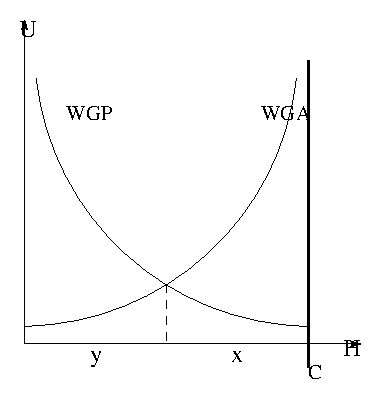
\includegraphics[width=0.49\textwidth]{images/Abbildungen/neuest5.eps}
		\caption{Arbeitsmarkt}
		\hfill \footnotesize\sffamily\textbf{Quelle:} eigene Darstellung
		\label{Grenzentlohnung}
		\vspace{0.48cm}
	\end{figure}

Dieser Zusammenhang wird in Abbildung \ref{Grenzentlohnung} dargestellt. Der Schnittpunkt beider Grenzprodukte der Sektoren 1 und 2 zeigt die Verteilung der Arbeitsplätze der gesamten Bevölkerung auf die jeweiligen Sektoren mit dem einheitlichen gleichgewichtigen Lohnsatz. 


\section[Mikroökonomisches Gleichgewicht]{Mikroökonomisches Gleichgewicht\sectionmark{mikroökonom. GG}}\label{sec:mikro GG}
\sectionmark{mikroökonom. GG}
Das Grundgerüst des Modells von \citet{Acemoglu.2006} wurde auch auf der mikroökonomischen Ebene übernommen. Es unterscheiden sich auch hier Manager hinsichtlich ihres Alters und ihrer technischen Qualitäten. Beides bedingt die Projektgrö{\ss}e, die ein Unternehmen durchführen darf. Für den Kapitalisten, der einen Arbeiter als Ingenieur  einstellt, ist letztendlich der resultierende Wert dieser Führungskraft, der durch ihn entstehende zusätzliche Gewinn, von Bedeutung. Bei der Auswahl des technischen Managers muss ein Kapitalist somit alle Kriterien berücksichtigen.\\
Die Qualifikationen, das Alter und die damit verbundene mögliche Projektgrö{\ss}e haben Einfluss auf die Produktivität, die Investitionssumme und letztlich den Gewinn eines Unternehmens. Die folgende Abbildung \ref{fig:technische Eigenschaften} liefert eine Übersicht über die möglichen Eigenschaften und Fähigkeiten eines Ingenieurs mit den entsprechenden Kombinationsmöglichkeiten.\\


	\begin{figure}[H]
		\vspace{0.43cm}
		\centering 
		\begin{tikzpicture}[node distance=1cm, auto]  
			\tikzset{
			mynode/.style={rectangle,rounded corners,draw=black, top color=white, bottom color=green!50,very thick, inner sep=1em, minimum size=3em, text centered},
			myarrow/.style={thick},
			mylabel/.style={text width=5em, text centered}, 
			myline/.style={shorten >=1pt, thick}
			}  
			\node[mynode] (unternehmer) {Ingenieur};  
			\node[below=2cm of unternehmer] (dummy) {}; 
			\node[mynode, left=of dummy] (JUNG) {jung};  
			\node[mynode, right=of dummy] (ALT) {alt};
			\node[mylabel, left=of JUNG] (label1) {Alter};  
			%\node[mylabel, below right=of unternehmer] (label2) {Participation rate $\theta_2$};
			% The text width of 7em forces the text to break into two lines. 
			\node[mynode, below=of JUNG](KLEIN){klein};
			\node[mynode, below=of ALT](GROSS){gro{\ss}};
			\node[mylabel, left=of KLEIN] (label2) {Projektgrö{\ss}e};  
			\node[mynode, below=of KLEIN](UNKNOWN){unbekannt};
			\node[mynode, below right=1.43cm of GROSS](HIGH){hoch};
			\node[mynode, left= of HIGH](LOW){gering};
			\node[mylabel, left=of UNKNOWN] (label3) {Qualifikation};  
			\node[mynode, below=of UNKNOWN](INNOVATIV){?innovativ?};
			\node[mynode, below=of LOW](LIQUIDE){liquide};
			\node[mynode, below=of HIGH](INNOQUIDE){\parbox{1.8cm}{innovativ\\ + liquide}};
			\node[mylabel, left=of INNOVATIV] (label4) {Potenzial};			
			\draw[myarrow] (unternehmer.south)  ++(0,0) -- ++(0,-1) -|  (JUNG.north);	
			\draw[myarrow] (unternehmer.south)  ++(0,0) -- ++(0,-1) -|  (ALT.north);
			\draw[myline] (JUNG.south) ++(0,0) -- ++(0,-1) -|  (KLEIN.north);	
			\draw[myline] (ALT.south) ++(0,0) -- ++(0,-1) -|  (GROSS.north);	
			\draw[myline] (KLEIN.south) ++(0,0) -- ++(0,-1) -|  (UNKNOWN.north);
			\draw[myarrow] (GROSS.south) -- ++ (0,0) -- ++(0,-.6) -|  (LOW.north);	
			\draw[myarrow] (GROSS.south) -- ++ (0,0) -- ++(0,-.6) -|  (HIGH.north);
			\draw[myline] (UNKNOWN.south) -- ++(0,0) -- ++(0,-1) -|  (INNOVATIV.north);
			\draw[myline] (LOW.south) -- ++(0,0) -- ++(0,-1) -|  (LIQUIDE.north);
			\draw[myline] (HIGH.south) -- ++(0,0) -- ++(0,-1) -|  (INNOQUIDE.north);
			%\draw[<->, >=latex', shorten >=2pt, shorten <=2pt, bend right=45, thick, dashed] 
			(JUNG.south) to node[auto, swap] {Competition}(ALT.south); 
			% The swap command corrects the placement of the text.
		\end{tikzpicture}\\
		%\medskip
		\hfill \footnotesize\sffamily\textbf{Quelle:} eigene Darstellung
		\caption{Eigenschaften eines Ingenieurs} 
		\label{fig:technische Eigenschaften}
	\end{figure}


Als Ingenieure angestellte Arbeiter werden als gut ausgebildete Personen mit ausgeprägten technischen Fähigkeiten kategorisiert, wenn $\gamma_t >1$ gilt. Weisen Arbeiter einen geringeren Bildungsstand auf, so sind sie mit weniger qualifizierenden technischen Fähigkeiten ausgestattet, sodass  $\gamma_t=0$ gilt. Bezüglich des qualitativen Bildungsstandes wird demzufolge zwischen hoher Qualifizierung der technischen Geschäftsführung durch eine modernere Bildung und eher traditionell und dann relativ weniger gut ausgebildeten technischen Managern bzw. Ingenieuren unterschieden.\\
Werden die Arbeiter neu eingestellt, so ist den Unternehmungen noch nicht bekannt, mit welchen Fähigkeiten die zukünftigen Ingenieur  ausgestattet sind. In diesem Fall handelt es sich um junge technische Geschäftsführer, die noch keine nennenswerte Berufserfahrung aufweisen können.\\ 
Die Wahrscheinlichkeit, dass der eingestellte Ingenieur mit hohen Fähigkeiten ausgestattet ist, beträgt $\lambda$ und mit einer Wahrscheinlichkeit von $(1-\lambda)$ ist die Ausbildung des Ingenieurs von geringer Qualität.\\
Weiterhin werden die Ingenieure neben ihren unternehmerischen und technischen Qualitäten auch anhand des Alters unterschieden. Haben die technischen Manager bereits eine Periode gearbeitet, werden sie als "`alt"' klassifiziert. Aufgrund der vorhandenen Erfahrung und der gemeinsamen Zusammenarbeit sind dadurch dem Unternehmen die Fähigkeiten der Angestellten bekannt.\\
Kategorisiert nach ihren Eigenschaften, sind die Ingenieure in zwei verschiedenen Unternehmensbereichen dienlich und bedingen damit die Strategie, denn es liegt an den Kenntnissen und Fähigkeiten der Ingenieure, ob ein Unternehmen sich auf die Imitation oder Innovation konzentriert. Innovationen können die Produktivität erhöhen und den Gewinn eines Unternehmens steigern, wozu qualifizierte Ingenieure notwendig sind. Ältere Ingenieure können hingegen die Kapitalisten durch ihre Einlage auch finanziell unterstützen. Diese Liquidität stellt ebenfalls einen Anreiz für das Unternehmen dar, da dies dem Ingenieur ermöglicht, die Projektgrö{\ss}e mit zu beeinflussen. Bei diesem Entscheidungsproblem entsteht ein Trade-off, der in Kapitel \ref{sec:Strategiewahl} noch relevant und dann genauer betrachtet wird.


\subsection{Finanzierung der Unternehmung}
Die hier aufgeführten Finanzierungsmöglichkeiten der Unternehmen wurden ebenfalls aus dem Modell von \citet{Acemoglu.2006} übernommen.
Die Eigentümer der Unternehmen, die Kapitalisten, benötigen zum einen Geld, um den Ingenieur sowie Arbeiter einzustellen und zum anderen, um die Finanzierung der Projekte zu gewährleisten. Ferner liegt ein unvollkommener Kapitalmarkt vor. \\
Eine monetäre Bezugsquelle ist der Kapitalist selbst. Dieser ist in der Lage, die grundlegenden Kosten zu decken, um kleine Projekte durchzuführen. Dabei handelt es sich nicht um Vermögen, welches von au{\ss}en in die Unternehmung bzw. in das Modell einflie{\ss}t. \\


Neben dem Kapitalisten kann auch der Ingenieur einen Beitrag zur finanziellen Situation des Unternehmens leisten. Die Finanzierungsart hängt wiederum von dem Alter der Unternehmen ab. Eine Neugründung hat eingeschränktere finanzielle Möglichkeiten als ein bereits bestehendes, erprobtes Unternehmen. In neu gegründeten Unternehmen können junge Kapitalisten  mit Hilfe von Darlehen die notwendigen Anfangsinvestitionen tätigen. Die Darlehen werden ihm von seinen Konkurrenten gewährt und stellen keine Markteintrittsbarriere dar. In diesem Fall ist auch der Ingenieur "`jung"' bzw. unerfahren und hat keine liquiden Mittel, die er in das Unternehmen einflie{\ss}en lassen kann.\\
Kapitalisten bestehender "`alter"' Firmen verfügen zusätzlich zu den Darlehen anteilig über die erwirtschafteten Gewinne vorheriger Projekte, die reinvestiert werden.\\
Die Möglichkeit, dass der angestellte Ingenieur die finanzielle Lage der Unternehmung verbessern kann, besteht nur bei bereits vorhandenen und somit etablierten Unternehmen, die ältere Ingenieure beschäftigen. Aus vorangegangenen Projekten erhielten die Ingenieure ein Gehalt mit darin enthaltener Gewinnbeteiligung. Nur mit Hilfe dieser Ersparnis aus der Gewinnbeteiligung können nun auch gro{\ss}e Projekte finanziert werden.\footnote{Die Notwendigkeit der Gewinnbeteiligung wird im folgenden Kapitel \ref{Moral Hazard und Gewinnbeteiligung} diskutiert.}\\


Es ist nur den Kapitalisten vorbehalten, Darlehen aufzunehmen. Die Ingenieure unterliegen Kreditbeschränkungen, weswegen die grö{\ss}ere Last der Investitionskosten durch den Kapitalisten getragen werden muss, obwohl dieser nur einen Anteil von $(1-\mu)$  der Gewinne erhält. 

\subsubsection{Moral Hazard und Gewinnbeteiligung}\label{Moral Hazard und Gewinnbeteiligung}


Als Folge des unvollkommenen Kapitalmarktes und indirekter Folgen des Moral Hazards können Unterinvestitionen durchgeführt werden. Es kann vorkommen, dass Unternehmen sich für kleinere Projekte entscheiden, obwohl höhere Investitionen aus sozialer Sicht effizienter wären. Gerade bei neu gegründeten Unternehmen muss der Kapitalist die vollen Investitionskosten allein tragen. In diesem Fall kommt es besonders häufig zu Unterinvestitionen, weil er nicht bereit ist, das gesamte Risiko für gro{\ss}e Projekte ohne die finanzielle Beteiligung der Mitarbeiter zu tragen.\\


In beiden Fällen können die Investitionsmöglichkeiten älterer Ingenieure das Problem mindern. Die angesprochene Gewinnbeteiligung resultiert in diesem Modell aus dem Umgang mit Moral Hazard. Es kommt zum Problem des Moral Hazards, wenn ein Wirtschaftssubjekt (Agent) besser über die eigenen Handlungen informiert ist, als das andere Individuum (Prinzipal), in dessen Auftrag diese Aufgaben und Pflichten erfüllt werden sollten. In diesem Fall ist es dem Kapitalisten, dem Prinzipal, nicht möglich die operativen und auch innovativen Anstrengungen des Ingenieurs, des Agenten,  zu bewerten und dessen vollen Arbeitseinsatz zu beurteilen. Diese Informationsasymmetrie führt zu dem Problem verzerrter Anreize. Der Agent erfüllt seine Verpflichtung mit möglicherweise minimalem Arbeitseinsatz, wohingegen dann dem Prinzipal aufgrund des Mangels an Sorgfalt unnötige Kosten entstehen. Da der Kapitalist die Arbeitsabläufe weder überwachen noch hinsichtlich sorgfältiger Ausführung kontrollieren kann, wird davon ausgegangen, dass der Agent anteilig Kosten $\mu$ verursacht.\footnote{Zu einem späteren Zeitpunkt wird ersichtlich, dass dieser Aufwand der Gewinnbeteiligung des Ingenieurs entsprechen muss.} Bei diesen Kosten kann es sich auch um veruntreute Gelder handeln, die für private Zwecke genutzt werden. Der Agent hat einen Anreiz, seinen eigenen Nutzen zu maximieren und fügt dabei dem Unternehmen einen finanziellen Schaden zu, der durch die Höhe von $\mu$ gemessen werden kann. Er zeigt auch gleichzeitig den Grad der Unvollkommenheit des Kapitalmarktes, die durch dieses Anreizproblem entsteht.\\ 


Gemindert werden kann dieses Problem aber nicht nur durch Mechanismen der Überwachung und Kontrolle, sondern auch durch eine neue Ausrichtung der Anreize. Der Agent muss die Auswirkungen des Problems selbst mit erleiden, um im eigenen Interesse sorgfältiger zu handeln. Dies kann durch eine Selbstbeteiligung wie bei Versicherungen oder in einem Unternehmen durch Gewinn- oder Umsatzbeteiligung gewährleistet werden. Dadurch ist der Agent motivierter, seine Aufgabe gründlicher und gewissenhafter zu erledigen, weil entstehende Kosten ihn nun selbst betreffen.\footnote{Beispiel Moral Hazard: Die Finanzkrise aus dem Jahr 2008 zeigt beispielhaft die möglichen Auswirkungen des Problems. Dabei führte der Moral Hazard zu einer Mentalität höherer Risikobereitschaft im amerikanischen Finanzsystem. Das Problem des Moral Hazard lag in den angedachten Bonuszahlungen für Bankenmanager. Sie versuchten, ihre jährliche Gewinnbeteiligung auszudehnen, indem risikoreiche Investitionen getätigt wurden, die einen deutlich höheren Gewinn versprachen. Da der Bankenmarkt immer mit staatlicher Unterstützung rechnen konnte, rechneten die Manager nicht mit weitreichenden Konsequenzen im Falle einer Fehlinvestition.}\\
%Text {Krugman 2010 #75S: 583–584} Fu{\ss}note:{Mankiw 2012 #76S: 574–575}
Für den Umgang mit diesem Problem haben auch \citet{Acemoglu.2006} im Rahmen dieses Modells eine Gewinnbeteiligung eingeführt. Den Agenten (Ingenieuren) steht nach einer Periode ein Anteil des Gewinns $\pi_t(\nu|s,e,z)$ zu.\\
Dabei beschreibt $s$ die Projektgrö{\ss}e, $e$ das Alter des Ingenieurs und $z$ die Qualifikationen dessen.\footnote{Die Parameter werden im folgenden Kapitel \ref{sec:Strategiewahl} noch einmal genauer erläutert und definiert.}  Aus der Gleichung  \eqref{Gewinn Zwischengutsektor} zusammen mit Gleichung \eqref{Produktivitat} ergibt sich:

	
	\begin{equation}
		\pi_t(\nu)=\delta s_t(\nu)[\eta\overline{A}_{t-1}+\gamma_t(\nu)A_{t-1}]N_t
	\end{equation}


Diese Gleichung bildet die direkte Abhängigkeit des Gewinns zu den Eigenschaften des Ingenieurs (Projektgrö{\ss}e, Alter und Ausbildung) ab.  Damit das Problem des Moral Hazards gemindert wird und die Unternehmer keine Erträge an sich nehmen, die ihnen nicht zustehen, muss deren Gehalt $W_t(\nu|s,e,z)$ grö{\ss}er sein als der Gewinnanteil $\mu\pi(\nu|s,e,z)$, der möglicherweise entwendet werden kann und es gilt demnach:


	\begin{equation}
		W_t(\nu|s,e,z)-\mu\pi(\nu|s,e,z)\geq 0
	\end{equation}


Diese Restriktion führt auch dazu, dass eine vertragliche Regelung, die eine Weiterbeschäftigung nur bei sorgfältiger und vollständiger Erfüllung der Aufgaben vorsieht, hinfällig wird. Denn wird der Ingenieur zusätzlich durch eine Gewinnbeteiligung vergütet, dann stellt dies einen Anreiz dar, jegliche Aufgaben und Pflichten gewissenhaft zu erledigen, um weiterhin im Unternehmen als Ingenieur angestellt zu bleiben. Der Ingenieur ist zudem motiviert, den Jahresumsatz und damit möglichst auch den Gewinn langfristig zu steigern, um seine persönliche Bonuszahlung zu erhöhen.\\


Die Gestaltung dieses Modells wird dadurch auf zwei Weisen beeinflusst. Moral Hazard führt hier zu Kreditbeschränkungen und schränkt damit das Investitionsvolumen vor allem junger Ingenieur ein, die keine Gewinnbeteiligung aus vorherigen Projekten haben. Sie können keine Sicherheiten vorweisen und ihre Liquidität ist geringer als die der älteren Ingenieure. Es können keine gro{\ss}en Projekte durchgeführt werden, die eine hohe Investitionssumme erfordern, weil ein junger Ingenieur nicht in Vorlage gehen kann.\\
Dies ist für die älteren, weniger qualifizierten Ingenieure von Vorteil und erhöht deren Wert für ein Unternehmen. Au{\ss}erdem schützen diese anteiligen Gewinnausschüttungen die traditionell ausgebildeten älteren Ingenieure davor, durch junge Ingenieure ersetzt zu werden. Die finanziellen Mittel steigern die Attraktivität und ermöglichen einen ausgeglicheneren indirekten Wettbewerb mit den möglichen hohen unternehmerischen und letztlich innovativen Fähigkeiten der jungen Ingenieure. Die Gewinnbeteiligung hat also in doppelter Art einen positiven Effekt auf das Unternehmen. Zum einen mindern sie die Veruntreuung von Geldern und zum andern können diese Mittel von den älteren Ingenieuren reinvestiert werden. Dadurch werden dem Unternehmen in einer zukünftigen Periode zusätzliche finanzielle Mittel zur Verfügung gestellt, um gro{\ss}e Projekte bearbeiten zu können. \\


Der ausgeschüttete Gewinn ist begrenzt durch die Kosten einer Investition, $\widehat{RE}_t(\nu|s,e,z)\leq k_t(\nu|s)$. Au{\ss}erdem unterliegen sie noch einer weiteren Restriktion:


	\begin{equation}
		0\leq\widehat{RE}_t(\nu|s,e,z)\leq RE_t(\nu|s,e,z)
	\end{equation}

Die gesamten Gewinnrücklagen eines Unternehmens $RE_t(\nu|s,e,z)$ müssen mindestens der Gewinnbeteiligung des Managers entsprechen. Dies verhindert beispielsweise zusätzliche Zahlungen des Ingenieurs an den Kapitalisten, was zu ungenauen Machtverhältnissen führen kann. \\


Letztlich führt die Minderung des Moral Hazard Problems durch die Einführung von Gewinnbeteiligungen zu einem Trade-off zwischen jungen, finanzschwachen und älteren, finanzstarken Ingenieuren. 


\subsection{Strategiewahl}\label{sec:Strategiewahl}
Das angedeutete Entscheidungsproblem ist Kern des mikroökonomischen Gleichgewichts und wird im Folgenden genauer erläutert. Die strategischen Hauptentscheidungen dieses Modells werden durch den Kapitalisten einer Unternehmung getroffen. Dabei spielen die Eigenschaften der angestellten Ingenieure und die damit verbundene Projektgrö{\ss}e eine wichtige Rolle. \\
Die unternehmerische Tätigkeit eines Angestellten gliedert sich in diesem Modell in zwei Aufgabenfelder. Zum einen sollen neue Technologien erfunden werden, wozu die Fähigkeiten und Qualifikationen wichtig sind. Zum anderen sollen bereits vorhandene Technologien der WTG nachgeahmt werden, wofür grundsätzlich keine speziellen Fachkenntnisse benötigt werden, wie es bei der Innovationsentwicklung erforderlich ist. 


\subsubsection{Imitative Tätigkeit}
Für die Imitation bereits bekannter Produktionstechniken oder Güter bedient sich ein Unternehmen dem Wissensstand der WTG und ahmt mit Hilfe dieser die Produkte oder Produktionsprozesse nach. Der Illustration dient wieder das Beispiel der Textilindustrie. Durch den Erwerb von Gütern der Konkurrenten können diese hinsichtlich ihrer Herstellungsprozesse studiert werden. Dabei kann festgestellt werden, dass beispielsweise eine neue stabilere Naht das Endprodukt verbessert und zu effizienteren Arbeitsabläufen führt. Hierfür ist die Qualität der Ausbildung der Ingenieure nicht so sehr von Bedeutung. Adaptive Tätigkeiten fordern lediglich eine genaue Beobachtungsgabe und die Beherrschung traditioneller Arbeitsweisen. In diesem Beispiel zählen der Umgang mit einer Nähmaschine und das Anfertigen von Schnittmustern zu diesen Grundfertigkeiten.


\subsubsection{Innovative Tätigkeit} 
%\textit{Innovative Tätigkeit}\\
Für die Erfindung neuer Prozesse ist es jedoch sehr wichtig, dass es sich um hoch qualifizierte Ingenieure handelt, da hier vor allem selbstständiges und vorausschauendes Denken vorausgesetzt wird. Die Entwicklung der angesprochenen Naht fordert neben den allgemeinen Grundkenntnissen auch Kenntnisse über die Beschaffenheit der Materialien wie Stoff, Faden und Nähmaschine sowie darüber hinaus noch die Fähigkeit, die Wirkung neuer Kombinationsmöglichkeiten zu erfassen. Ziel der innovativen unternehmerischen Tätigkeiten ist das Erkennen vorhandener Probleme und eine daraus folgende Problemlösung. 


\subsubsection{Entscheidungsprozess}
Wenn sich der Kapitalist dazu entscheidet junge Ingenieure einzustellen, so ist es unvorhersehbar, welche Qualifikationen diese mit sich bringen. Sind die Fähigkeiten eines Ingenieurs bekannt, kann über dessen Entlassung oder dessen Verbleib im Unternehmen entschieden werden. Für ältere, hoch qualifizierte Ingenieure besteht ein Nachfrageüberschuss, sie werden nicht mehr aus einem Unternehmen entlassen. Denn gerade das benötigte Know How und somit das Potenzial, technischen Fortschritt zu generieren, ist sehr profitabel und beliebt. Es ist zu entscheiden, ob ein erfahrener Ingenieur mit geringer Qualifikation in dem Unternehmen bleiben soll oder nicht. Der Entscheidungsfindung dient eine genaue Analyse beider Alternativen, anhand der Abschätzung der resultierenden Wertigkeiten der Ingenieure für das jeweilige  Unternehmen.\\
Zunächst wird der Wert jeder Alternative einzeln betrachtet. Dabei gilt in diesem Modell, dass ein Ingenieur entweder jung oder alt ist mit $e\in\left\{Y,O\right\}$. Die Qualifikation bemisst sich an der Art der Ausbildung, die gut bzw. modern sein kann oder eher schlecht damit traditionell geprägt ist, mit $z\in\left\{L,H\right\}$. Au{\ss}erdem hängt der Wert einer Alternative von der Projektgrö{\ss}e ab, die gro{\ss} oder klein sein kann, $s\in\left\{\sigma_j,1\right\}$.


	\begin{equation}
		V_{tj} (\nu|s=1,e=O,z=L)=[(1-\mu)\delta_j N_j \eta\overline{A}_{t-1}-max(\kappa\overline{A}_{t-1}-RE_t,0)]\label{Wert}
	\end{equation}


Gleichung \eqref{Wert} gibt den Wert älterer, traditionell ausgebildeter Ingenieur an, die gro{\ss}e Projekte bearbeiten. Dieser setzt sich zusammen aus dem erwirtschafteten Gewinn durch imitative Tätigkeiten $\delta_j N_j \eta\overline{A}_{t-1}$, abzüglich dem ausgeschütteten Gewinn an die Ingenieure $\mu\delta_j N_j \eta\overline{A}_{t-1}$ und der maximalen Kosten $\kappa\overline{A}_{t-1}-RE_t$. Dabei wird im Folgenden davon ausgegangen, dass die Kosten des Projekts die eingebrachten Gewinne $RE_t$ überschreiten, $\kappa\overline{A}_{t-1}>RE_t$. Diese älteren Ingenieure sind grö{\ss}tenteils für nachahmende Prozesse geeignet und scheinen zunächst weniger attraktiv. Doch durch das Einbringen ihrer gesparten Gewinnanteile steigern sie ihren Marktwert. Denn der unvollkommene Kapitalmarkt führt bei den Unternehmen, zu grö{\ss}eren Investitionen und damit wird die Durchführung gro{\ss}er Projekte ermöglicht. Die Vorzüge grö{\ss}erer Projekte liegen in höheren erwarteten Gewinnen, jedoch ist auch mit höheren Kosten zu rechnen. Grö{\ss}ere Projekte führen gemä{\ss} \eqref{Produktivitat} zu einer höheren Produktivität, weil Unterinvestitionen vermieden werden und dadurch die Effizienz gefördert wird, obwohl weniger qualifizierte Ingenieure nicht innovativ tätig sind. 


	\begin{equation}
		E_tV_{tj} (\nu|s=\sigma_j,e=y)=(1-\mu)\delta_j N_j\sigma_j(\eta +\lambda\gamma a_{j t-1})\overline{A}_{t-1}-\phi\kappa\overline{A}_{t-1}\label{erwarteter Wert}
	\end{equation}

Gleichung \eqref{erwarteter Wert} ist die formale Darstellung des erwarteten Marktwertes junger Ingenieure und setzt sich wie folgt zusammen: 
Von dem jeweiligen möglichen Gewinn aus Imitation $\eta\delta_j N_j\sigma_jv$ bzw. Innovation $\lambda\gamma a_{j t-1}\delta_j N_j\sigma_j$ werden jeweils die Gewinnbeteiligungen der Ingenieure $-\mu\delta_j N_j\sigma_j(\eta +\lambda\gamma a_{j t-1})$ subtrahiert. Von diesem Ertrag werden noch die Kosten in Höhe von $\phi\kappa\overline{A}_{t-1}$ abgezogen. 

Die Untersuchung junger Ingenieure deren Fähigkeiten noch unbekannt sind, zeigt, dass der Kapitalist die Finanzierung der Projekte allein realisieren muss. Das Unternehmen kann keine ersparten Gewinnbeteiligungen dieser Mitarbeiter beziehen, weil es sich um relativ junge und somit unerfahrene Ingenieure handelt. \\
Mit einer Wahrscheinlichkeit von $(1-\lambda)$ handelt es sich um einen weniger qualifizierten Manager. Stellt sich jedoch heraus, dass der junge Ingenieur hohe Qualifikationen mit sich bringt, könnte der Aspekt der fehlenden Ersparnis durch innovative Tätigkeiten ausgeglichen werden. Ein höherer Bildungsstand und damit verbundener technischer Fortschritt nutzt der Unternehmung ebenso wie die Durchführung gro{\ss}er Projekte. Durch Innovationen steigt in der Regel auch die Absatzmenge an, selbst wenn insgesamt das Verkaufsvolumen kleinerer Projekte geringer ist. \\
Nachdem beide Möglichkeiten analysiert wurden, muss das Unternehmen abwägen, ob es einen alten, erfahrenen Ingenieure mit traditioneller Ausbildung behalten möchte oder diesen durch einen jungen Ingenieur ersetzt. Es stellt sich also die Frage, ob die Investitionen älterer Ingenieure attraktiver sind als die möglichen innovativen Fähigkeiten eines neuen Ingenieurs. Damit sich ein Unternehmen gegen die Entlassung erfahrener, traditionell ausgebildeter Ingenieure entscheidet, muss  Ungleichung \eqref{Wertvergleich} gelten, in der die Wertigkeit beider Alternativen gegeneinander abgewogen wird.


	\begin{equation}
		V_{tj}(\nu|s=1,e=o,z=L) > E_t V_{tj} (\nu|s=\sigma_j,e=y)\label{Wertvergleich}
	\end{equation}


Der Wert eines älteren, schlecht ausgebildeten Ingenieurs, mit dessen Hilfe gro{\ss}e Projekte finanziert werden können, muss höher sein als der erwartete Marktwert, wenn das Unternehmen einen jungen Ingenieur einsetzt, mit dem kleine Projekte realisiert werden und dessen Fähigkeiten noch unbekannt sind. Ist dies nicht der Fall, wird der Ingenieur entlassen und ein junger Mitarbeiter wird neu eingestellt, weil es für das Unternehmen nicht mehr lohnend ist, den älteren Ingenieur weiter zu beschäftigen. \\
Die eingebrachten Gewinnbeteiligungen der Ingenieure müssen die höheren Kosten grö{\ss}erer Projekte kompensieren können und sogar höher sein, als die Gewinne, die in kleinen, möglicherweise innovativ ausgerichteten Projekten realisiert werden, damit das Arbeitsverhältnis bestehen bleibt. \\
Bei dieser Personalentscheidung werden die erfahrenen, hoch qualifizierten Mitarbeiter nicht berücksichtigt, da diese am "`beliebtesten"' sind und die Unternehmensstruktur mit innovativen Tätigkeiten prägen sowie zur Finanzierung gro{\ss}er Projekte beitragen.\\
Diese Rangfolge spiegelt sich auch in der Gehaltsstruktur wieder. Die Entlohnung der älteren, hoch qualifizierten Ingenieure ist höher, als die der älteren, weniger gut ausgebildeten und letztlich erzielen die jungen Ingenieure das geringste Einkommen.



\section[Makroökonomisches Gleichgewicht]{Makroökonomisches Gleichgewicht\sectionmark{Makroökonom. GG}}\label{sec:makro GG}
\sectionmark{Makroökonom. GG}
%dann im makro GG, wenn gilt: Volkseinkommen $=$ BIP
Beim makroökonomischen Gleichgewicht werden die mikroökonomischen Entscheidungen der Unternehmen akkumuliert. Dies bedingt die durchschnittliche Produktivität eines Landes und die daraus resultierende Lage zur WTG. Folglich ist die LTG äquivalent mit der Produktivität des führenden Unternehmens eines Zwischengutsektors, $A^H \Leftrightarrow A_t(\nu)$.\\
Der Abstand zur WTG wird in diesem Kapitel, so wie auch bei \citet{Acemoglu.2006}, mit Hilfe der durchschnittlichen Produktivität \eqref{Produktivitat} eines Landes ermittelt.
Diese ergibt sich aus den Entscheidungsalternativen der Kapitalisten. Im Folgenden werden die möglichen Produktivitäten eines Unternehmens erläutert, abhängig von der bisherigen personellen Besetzung und Strategiewahl. Dabei wird zwischen drei Möglichkeiten unterschieden: 1. die Unternehmen beschäftigen nur junge Ingenieure, 2. sie nehmen keine Personalveränderungen vor oder 3. die Unternehmen nehmen Personalveränderungen vor, indem weniger qualifizierte Ingenieure gegen junge ausgetauscht werden.\\
Im ersten Fall werden die neu gegründeten Unternehmen betrachtet, die nur junge, unerfahrene Ingenieur einstellen können. Die Fähigkeiten der Ingenieure sind ungewiss und mit einer Wahrscheinlichkeit von $\lambda$ relativ hoch und mit einer Wahrscheinlichkeit von $(1-\lambda)$ relativ gering.


	\begin{equation}
		A_{tj}^{y}=\sigma_j(\eta\overline{A}_{t-1}+\lambda\gamma A_{t-1})\label{Produktivitat jung}
	\end{equation}


Die Produktivität der jungen Ingenieure $A_{tj}^{y}$ ist in erster Linie von der Qualifikation der Ingenieure abhängig. Das Wissen der LTG $A_{t-1}$ kann nur durch die qualifizierten, innovativ arbeitenden Ingenieure, $\gamma$, mit einer Wahrscheinlichkeit von $\lambda$ genutzt werden.\footnote{Es werden Innovationen mit einer Wahrscheinlichkeit von $\lambda$ entwickelt. Dem Gesetzt der gro{\ss}en Zahl folgend entspricht $\lambda$ der Anzahl der Sektoren, die erfolgreich innovieren, also der Häufigkeit von Innovationen in einer Periode.} Das lokale technische Wissen der Vorperiode $\overline{A}_{t-1}$ steht allen Ingenieuren der Volkswirtschaft zur Verfügung und dient der Imitation von Gütern und Prozessen. Bei $\eta$ handelt es sich um die Imitationsintensität, die angibt wie stark sich die Technologie verändert hat und wie intensiv die Technologien der WTG eingesetzt wird.\\


Bei der 2. und 3. Entscheidungsmöglichkeit handelt es sich um die Produktivität älterer Unternehmen, die seit mindestens einer Periode Ingenieure angestellt haben und es zu entscheiden gilt, ob die weniger gut ausgebildeten Ingenieure weiterhin angestellt bleiben $A_{tj}^{o}[R_{tj}=0]$ oder durch junge ersetzt werden $A_{tj}^{o}[R_{tj}=1]$. \\


Die Wahl der jeweiligen Alternative wird durch das mikroökonomische Gleichgewicht determiniert. Wird sich für die Weiterbeschäftigung aller Ingenieure eingesetzt, besteht die Ingenieurstruktur aus Ingenieuren beider Bildungsschichten. Die Erfahrung aller und die finanzielle Unterstützung der Ingenieure ermöglicht es nur noch gro{\ss}e Projekte durchzuführen mit $s=1$.


	\begin{equation}
		A_{tj}^{o}[R_{tj}=1]=\eta\overline{A}_{t-1}+\lambda\gamma A_{t-1}\label{Produktivitat nur alte}
	\end{equation}


Bei der anderen Alternative werden nur die weniger qualifizierten Ingenieure entlassen. Die hoch qualifizierten verbleiben im Unternehmen und bearbeiten gro{\ss}e Projekte. Wohingegen die nun neu eingestellten jungen Unternehmen mit kleineren Projekten, $s=\sigma_j$, vertraut werden. 


	\begin{equation}
		A_{tj}^o[R_{tj}=0]=\lambda(\eta\overline{A}_{t-1}+\gamma A_{t-1})+(1-\lambda)\sigma_j(\eta\overline{A}_{t-1}+\lambda\gamma A_{t-1})\label{Produktivitat alt und jung}
	\end{equation}


Es wird angenommen, dass es sich bei der Hälfte aller Unternehmen um Neugründungen handelt. Dabei wird die Gesamtheit aller Produktivitäten eines Sektors und somit aller Unternehmen eines Sektors in einem Land betrachtet. 


	\begin{equation}
		A_{tj}\equiv\int_0^1 A_{t}(\nu)d\nu=\frac{(A_{tj}^y+A_{tj}^o)}{2} \label{Produktivitat gesamt}
	\end{equation}


Nachdem nun die Produktivität eines Landes beleuchtet wurde, wird die Wachstumsrate der aggregierten Produktivität $\frac{A_t}{A_{t-1}}$ genauer definiert die sich aus den Gleichungen \eqref{Produktivitat} und \eqref{durchschnittliche Technologie} ergibt.


	\begin{equation}
		\frac{A_t}{A_{t-1}}\equiv\frac{\int_0^1A_{t}(\nu)d\nu}{A_{t-1}}=\int_0^1s_{tj}(\nu)\left[\eta\frac{\overline{A}_{t-1}}{A_{t-1}}+\gamma_t(\nu)\right]d\nu
		\label{WachstumTechnologie}
	\end{equation}


Dieser Term beschreibt die Bedeutung des Abstandes zur WTG für den technologischen Fortschritt, der wiederum definiert ist als: 


	\begin{equation}
		a_{tj}\equiv\frac{A_{tj}}{\overline{A}_{tj}}\label{kleinA}
	\end{equation}


Ist der Quotient $\frac{\overline{A}_{t-1}}{A_{t-1}}$ aus Gleichung \eqref{WachstumTechnologie} relativ hoch, dann wird das technische Wachstum hauptsächlich durch imitative Tätigkeiten generiert, das Land liegt dann relativ weit von der WTG entfernt. Je kleiner der Abstand zur WTG, desto unbedeutender sind nachahmende Prozesse für die Produktivität eines Landes. Die Bedeutung von Innovationen ist dann deutlich höher und die Fähigkeiten des Ingenieurs $\gamma$ beeinflussen den Fortschritt wesentlich.\footnote{Eine abnehmende Annäherung an die WTG wird gewährleistet, wenn $\lambda\gamma<1$ gilt.}
Mit sinkender Distanz zur WTG nimmt die Bedeutung der Innovationsstrategie zu und damit wird auch eine zielgerichtete Wahl geeigneter Ingenieure wichtiger, wodurch sich der Schwerpunkt auf kurzfristige Beschäftigungsbeziehungen verlagert.\\


Für die Berechnung des Abstandes zur WTG \eqref{kleinA} werden die Gleichungen \eqref{Produktivitat jung}-\eqref{Produktivitat gesamt} zusammengefasst und ergeben sich für jeden Sektor folgende technologische Entwicklungsstände.\footnote{Die detaillierte Berechnung ist in Appendix \ref{sec:Abstand WTG} zu finden.}


	\begin{equation}
		a_{tj}=\begin{cases}\frac{1+\sigma_j}{2(1+g)}[\eta+\lambda \gamma a_{t-1j}] \hfill\text{if  } R_{tj}=1 \\
		\frac{1}{2(1+g)}[(\lambda+\sigma_j+(1-\lambda)\sigma_j)\eta+(1+\sigma_j+(1-\lambda)\sigma_j)\lambda\gamma a_{t-1 j}] \quad\hfill\text{if   }R_{tj}=0
		\end{cases}\label{Abstand WTG}
	\end{equation}


Jeweils der erste Summand in den eckigen Klammern steht für die nachahmenden Tätigkeiten. Der Vergleich beider Strategien zeigt, dass Wachstum, welches durch Imitationen bei der Strategie der Haltung weniger qualifizierter Manager resultiert, höher ist als das Wachstum bei der Strategie des Austauschs der Ingenieure.

 
	\begin{equation}
		(1+\sigma_j)\eta>(\lambda+\sigma_j+(1-\lambda)\sigma_j)\eta
	\end{equation}


Der zweite Summand beschreibt das Wachstum, das jeweils durch die Innovatiion hervorgerufen wird. Das Ersetzen älterer, weniger qualifizierter Ingenieure durch junge Ingenieure führt zu einem deutlich höheren Wachstum an technologischem Wissen, als es der Fall ist, wenn die Situation im Unternehmen unverändert bleibt und es keine Neueinstellungen gibt.


	\begin{equation}
		(1+\sigma_j)\lambda \gamma a_{t-1j}<(1+\sigma_j+(1-\lambda)\sigma_j)\lambda\gamma a_{t-1j}\footnote{Dies gilt ausgehend von dem Gleichen technologischen Entwicklungsstand $a_{t-1j}$.}
	\end{equation}


Von nun an wird die eben zuerst genannte Strategie der Unternehmen, welche vorwiegend die nachahmenden Tätigkeiten beinhaltet, als Investitions- oder Imitationsstrategie bezeichnet. Die Unternehmensstruktur ist durch gro{\ss}e Projekte geprägt, deren Finanzierung durch die eingebrachten Gewinnbeteiligungen der älteren, weniger qualifizierten Ingenieure ermöglicht wird. Die damit verbundenen hohen Investitionssummen sind unabhängig von der Entwicklung neuer Prozesse oder Produkte. Die Arbeitsabläufe einer Imitation sind relativ schlichter, unkomplizierter und strukturierter, somit sind hohe Qualifikationen des Ingenieurs von geringerer Bedeutung. Die Situation im Unternehmen bleibt in der zweiten Periode unverändert. Es stehen vor allem langfristige Beziehungen von Unternehmen zu Managern im Vordergrund, um das Investitionsvolumen möglichst hoch zu halten. Nicht nur die Erfahrung aller Angestellten, sondern auch resultierende Skaleneffekte aufgrund grö{\ss}erer Produktionsmengen sind ma{\ss}geblich für die Produktivität dieser Unternehmen.\\


Bei der zweiten Strategie wird der Begriff der Innovationsstrategie analog verwendet. Die gering qualifizierten Ingenieur werden entlassen, da diese höhere Kosten verursachen und durch sie der technologische Fortschritt des Unternehmens gehemmt wird. Der geringere Bildungsstand lässt nur nachahmende Tätigkeiten zu und ist somit nicht im Sinne der Innovationsstrategie. Diese Strategie ist durch kurzfristige Beziehungen geprägt und eine hohe Fluktuation der Ingenieure ist die Regel. Es ist den Kapitalisten wichtig, möglichst viele qualifizierte Ingenieure anzustellen. Dafür sind sie bereit, auf die finanziellen Mittel der traditionell ausgebildeten Ingenieure zu verzichten. Neue Ideen führen zu neuen Produktvarianten. Au{\ss}erdem kann durch Verbesserungsvorschläge die Effizienz der Produktion erhöht werden. Neben Start-up-Unternehmen finden junge Ingenieure nur in Firmen, die der Innovationsstrategie folgen eine Anstellung.

\subsection{Gesamtwirtschaftliche strategische Entscheidung bei exogener WTG im technologisch kleinen Land}

Nachdem beide Strategien vorgestellt wurden, hat jedes Unternehmen die Wahl sich für eine der beiden zu entscheiden. In einem technologisch kleinen Land haben Mikroinnovationen keinen Einfluss auf die WTG, die somit exogen gegeben ist. Demzufolge unterscheidet sich auch der mögliche Entwicklungspfad eines technologisch kleinen Landes von einem technologisch gro{\ss}en Land, das Makroinnovationen herstellen kann. Abbildung \ref{fig:ein Sektor exogene WTG} stellt die Abhängigkeit der heutigen technologischen Entwicklungssituation $a_t$ vom gestrigen Entwicklungsstand $a_{t-1}$ dar. Beide Strategien aus Gleichung \eqref{Abstand WTG} sind hier wiederzufinden.\newline


		\begin{figure}[H] 
			\vspace{0.13cm}
			\centering 
			\psfrag{a}{$a$}
			\psfrag{t}{  $_t$}
			\psfrag{-}{  $_-$}
			\psfrag{1}{\, $_1$}
			\psfrag{0.0}[c]{\scriptsize{0}}
			\psfrag{0.2}[c]{\scriptsize{0.2}}
			\psfrag{0.4}[c]{\scriptsize{0.4}}
			\psfrag{0.6}[c]{\scriptsize{}}
			\psfrag{0.8}[c]{}
			\psfrag{1.0}[c]{\scriptsize{1}}
			\begin{overpic}[width=0.9\textwidth]{images/Abbildungen/einSektorExo.eps}
				\put(10.5,0.5){\textcolor{black}{$a_r$}}
				\put(74.5,0.2){\textcolor{black}{$\hat{a}_t$}}
				\put(57.8,-1){\color[rgb]{0.74,0.97,0.22}{$\tilde{a}_{R=1}$}}
				\put(60.1,0.5){\color[rgb]{0,0.32,0}{$\tilde{a}_{R=0}$}}
				%\put(-0.4,12.5){\textcolor{black}{\scriptsize{0.2}}}
				\put(-0.4,34.5){\textcolor{black}{\scriptsize{0.6}}}
				\put(-0.4,45.5){\textcolor{black}{\scriptsize{0.8}}}
				\put(12.8,19.3){\color[rgb]{0,0.32,0}{\textcolor[rgb]{0.74,0.97,0.22}{Innovations-}}}
				\put(12.8,17.1){\color[rgb]{0,0.32,0}{\textcolor[rgb]{0.74,0.97,0.22}{strategie}}}
				\put(5,30){\color[rgb]{0,0.32,0}{\textcolor[rgb]{0,0.32,0}{Imitationsstrategie}}}
			\end{overpic}\\
			\hfill\footnotesize\sffamily{\textbf{Quelle:}}  eigene Darstellung
			\caption{ein Sektor bei exogener Welttechnologiegrenze}
			\label{fig:ein Sektor exogene WTG}
		\end{figure}
		
		
Die Situation ist nur für einen Sektor dargestellt. Die Firmen haben die Wahl zwischen der Imitations- und Innovationsstrategie. Jede Strategie ist durch eine Gerade abgebildet. Diese zeigt die technologische Entwicklung des Sektors bei entsprechender Strategie. Je nach technologischem Entwicklungsstand ist die eine oder die andere Strategie geeigneter, führt also zu einem höheren zukünftigen Entwicklungsstand.\\ 
Der folgende Abschnitt beschreibt drei mögliche Grenzwerte von $a_{t-1}$: $\hat{a}_t$, $a_r$ und $\tilde{a}$.  Bei $\hat{a}_t$ handelt es sich um den Schnittpunkt beider Strategien: Dies zeigt also, ab welchem Entwicklungsstand die Innovationsstrategie zukünftig zu einer höheren Produktivität führt.
Mit dem Überschreiten von $\hat{a}_t$ ist das technologische Wachstum durch die \textcolor[rgb]{0.74,0.97,0.22}{Innovationsstrategie} höher, als durch die bis dahin sinnvollere \textcolor[rgb]{0,0.32,0}{Imitationsstrategie}. 
Für Länder mit einem technologischen Entwicklungsstand, der also grö{\ss}er ist als $\hat{a}_t$, reduziert sich der Abstand zur WTG durch Innovationen schneller, als dies mit der \textcolor[rgb]{0,0.32,0}{Imitationsstrategie} der Fall wäre.\\
Ist der Entwicklungsstand eines Landes höher als der Schwellenwert, dann ist der entgangene zusätzliche Gewinn, hier die Produktivität, durch die relativ schlecht ausgebildeten Ingenieure, die im Unternehmen gehalten werden, zu hoch. Trotz der eingebrachten Gewinnbeteiligung sind junge Ingenieure dem Unternehmen mehr wert. Ist ein Land jedoch noch relativ wenig weit entwickelt und der Abstand zur WTG ist kleiner als $\hat{a}_t$, so ist die \textcolor[rgb]{0,0.32,0}{Imitationsstrategie} ratsam.\\
Nach der Produktivität stehen bei dem zweiten Grenzwert $a_r$ die Gewinne der Unternehmen im Vordergrund. Dieser Schwellenwert wird unter Berücksichtigung der verursachten Kosten der angestellten Ingenieure hergeleitet.\footnote{Die formale Herleitung ist in Appendix \ref{SchwellenwertAr} aufgeführt.}


	\begin{equation}
		a_r{_j}(\mu,\delta)=\frac{[(1-\mu)(1-\sigma_j)+\frac{1+r}{1+g}\mu\sigma_j]\eta-\frac{\kappa(1-\phi)}{\delta N_j}}{(1-\nu)\sigma_j\lambda\gamma} \label{Schwellenwert Kosten}
	\end{equation}


Der Wert $a_r$ gibt an, ab wann es profitabler ist, die Beziehung zu weniger qualifizierten Mitarbeitern zu beenden. Wird dieser überschritten, sind die älteren, weniger qualifizierten Ingenieure trotz der eingebrachten Gewinnbeteiligung zu teuer und es ist lohnender, junge unerfahrene Ingenieure einzustellen. Auch bei diesem Schwellenwert geht es um den Zeitpunkt des Strategiewechsels, jedoch aus einer anderen Perspektive.\\
Die beschriebene und dargestellte Situation entspricht der eines technologisch kleinen Landes bei einer exogenen WTG. Das Unternehmen, welches die Technologie der WTG bereitstellt, arbeitet mit grö{\ss}eren Projekten als das betrachtete Land. Demnach ist es mit kleineren Projekten nicht möglich, dieses Land einzuholen und die WTG zu erreichen.\\ Ein weiterer Grenzwert hinsichtlich des Entwicklungsstandes ist die Nicht-Konvergenz-Falle $\tilde{a}$. In weniger weit entwickelten, technologisch kleinen Ländern führen sehr kleine Projektgrö{\ss}en sowohl mit der Innovations- als auch mit der Imitationsstrategie zu einem technischen Wissenszuwachs. Langfristig konvergieren diese Länder jedoch bis zu einem maximal erzielbaren Wissensstand $\tilde{a}$, der unabhängig von der WTG ist. Anders ausgedrückt können diese Länder nicht zur WTG konvergieren, hier handelt es sich demnach um eine Nicht-Konvergenz-Falle. 
Die Erklärung der Situation für Länder, die mit einem Abstand zur WTG $a_{t-1}>\tilde{a}$ starten, ist etwas komplexer bzw. diffiziler. Zum einen ist fraglich, wie diese technologisch kleinen Volkswirtschaften diesen relativ hohen technologischen Entwicklungsstand erreicht haben. Handelt es sich um Länder in einer Krisensituation, ist es durchaus denkbar, dass sich durch die Verschlechterung der allgemeinen Situation auch die hier angesprochenen Investitionen mindern und dies zu einem Rückgang des technischen Wissens führen könnte. Dann wäre es ihnen kaum noch möglich, Bildungs- und Forschungseinrichtungen aufrecht zu erhalten und es würde  langfristig an der finanziellen Umsetzung von Innovationen und Imitationen scheitern, so dass auch diese Länder in der Nicht-Kovergenz-Falle $\tilde{a}$ münden. Zum anderen könnte es sich auch um Länder handeln, die sehr wahrscheinlich das Wachstum der WTG beeinflussen und hier als obsolet gelten.\\
Je nachdem welche Strategie verfolgt wird, ist einer der beiden folgenden Grenzwerte für $\tilde{a}$ ma{\ss}geblich.\footnote{Die formale Herleitung ist in Appendix \ref{NichtKonvergenzFalleImitation} und \ref{NichtKonvergenzFalleInnovation} zu finden.}


	\begin{equation}
		\tilde{a}_{R=1}=\frac{(1+\sigma_j)\eta}{2(1+g)-\lambda\gamma(1+\sigma_j)}\label{eq:aTilde1}
	\end{equation}


	\begin{equation}
		\tilde{a}_{R=0} = \frac{(\lambda+\sigma+(1-\lambda)\sigma)\eta}{2(1+g)-(1+\sigma+(1-\lambda)\sigma)\lambda\gamma}\label{eq:aTilde0}
	\end{equation}


Die Nicht-Konvergenz-Falle, oder der maximal mögliche Wissensstand $\tilde{a}$ ist in Abbildung \ref{fig:ein Sektor exogene WTG} bei der Innovationsstrategie höher als bei der Imitationsstrategie. Dadurch, dass $a_r<\tilde{a}$ gilt, ist es zwar wirtschaftlicher für die Volkswirtschaft der Innovationsstrategie zu folgen, führt jedoch zu einem geringeren maximal erzielbaren Entwicklungsstand $\tilde{a}_{R=1}$. Durch die Innovationsstrategie kann zwar durch Monopolmacht ein höherer Gewinn erzielt werden, jedoch führt diese zwischen $a_r$ und $\hat{a}_t$ zu einer geringeren Produktivität hinsichtlich des technologischen Fortschritts. Diese geringere Produktivität begründet auch warum ein geringerer technologischer Wissensstand erreicht wird, als mit der Imitationsstrategie. 

Wie aus den Gleichungen \ref{eq:aTilde1} und \ref{eq:aTilde0} ersichtlich ist, variiert die Nicht-Konvergenzfalle mit der Projektgrö{\ss}e.
\newpage
\subsection{Gesamtwirtschaftliche strategische Entscheidung bei endogener WTG im technologisch gro{\ss}en Land}
In technologisch gro{\ss}en Ländern handelt es sich um eine endogene WTG, dann verändert jede Innovation die WTG. Diese Situation ist in Abbildung \ref{fig:ein Sektor endogene WTG} dargestellt.


		\begin{figure}[htb]
			\vspace{0.13cm} 
			\centering 
			\psfrag{a}{$a$}
			\psfrag{t}{  $_t$}
			\psfrag{-}{  $_-$}
			\psfrag{1}{\, $_1$}
			\psfrag{0.0}[c]{\scriptsize{0}}
			\psfrag{0.2}[c]{\scriptsize{0.2}}
			\psfrag{0.4}[c]{\scriptsize{0.4}}
			\psfrag{0.6}[c]{\scriptsize{0.6}}
			\psfrag{0.8}[c]{\scriptsize{}}
			\psfrag{1.0}[c]{\scriptsize{}}
			\begin{overpic}[width=0.9\textwidth]{images/Abbildungen/einSektorEndo.eps}
				\put(23.6,0.4){\textcolor{black}{$a_r$}}
				\put(72.2,-0.1){\textcolor{black}{$\hat{a}_t$}}
				\put(90,0.3){\color[rgb]{0.74,0.97,0.22}{$\tilde{a}_{R=1}$}}
				\put(87,-1.2){\color[rgb]{0,0.32,0}{$\tilde{a}_{R=0}$}}
				%\put(-0.4,12.5){\textcolor{black}{\scriptsize{0.2}}}
				%\put(-0.4,34.5){\textcolor{black}{\scriptsize{0.6}}}
				\put(-0.4,45.5){\textcolor{black}{\scriptsize{0.8}}}
				\put(1,56){\textcolor{black}{\scriptsize{1}}}
				\put(5,20){\color[rgb]{0,0.32,0}{\textcolor[rgb]{0.74,0.97,0.22}{Innovations-}}}
				\put(5,17.8){\color[rgb]{0,0.32,0}{\textcolor[rgb]{0.74,0.97,0.22}{strategie}}}
				\put(5,36){\color[rgb]{0,0.32,0}{\textcolor[rgb]{0,0.32,0}{Imitationsstrategie}}}
				\end{overpic}\\
			\hfill\footnotesize\sffamily{\textbf{Quelle:}}  eigene Darstellung
			\caption{ein Sektor bei endogener Welttechnologiegrenze}
			\label{fig:ein Sektor endogene WTG}
		\end{figure}


Abhängig von der Investitionsgrö{\ss}e und von dem technologischen Entwicklungsstand kann die WTG erreicht und gebildet werden. Die Innovationsstrategie zeigt einen Entwicklungspfad auf, der zwingend in der WTG endet, demnach gilt $\tilde{a}_{R=1}=1$. Jedoch ist zu berücksichtigen, dass diese mit jeder weiteren Innovation angepasst wird. Das hier dargestellte Beispiel zeigt, dass es vor allem für noch weniger weit entwickelte Länder, mit einem gro{\ss}en Abstand zur WTG, die \textcolor[rgb]{0,0.32,0}{Imitationsstrategie} zu einem höheren technologischen Entwicklungsstand führt als die \textcolor[rgb]{0.74,0.97,0.22}{Innovationsstrategie}. Der Wechsel zur \textcolor[rgb]{0.74,0.97,0.22}{Innovationsstrategie} führt ab einem Entwicklungsstand von ca. $78\%$ zur WTG, dem Grenzwert $\hat{a}_t$, zu einem höheren technischen Fortschritt. Wird wieder die Rentabilität der Strategien berücksichtigt, dann findet ein deutlich früherer Wechsel zur Innovationsstrategie statt bei $a_r$.

\section{Handel}\label{sec:Handel}
Unter Einbeziehung des Au{\ss}enhandels müssen im wesentlichen wieder die drei Effekte betrachtet werden.

	\begin{description}
		\item [1] Marktgrö{\ss}eneffekt 
		\item [2] Wissens-Spillover-Effekt
		\item [3] Wettbewerbseffekt
	\end{description}
		
Die Monopole der Zwischengüterproduktion können in offenen Volkswirtschaften höhere Gewinne erzielen, als in einem geschlossenen Land, bedingt durch den Marktgrö{\ss}eneffekt. Die Öffnung für Handel führt bezüglich der Sektoren zu unterschiedlichen Entwicklungen. Zwischengüterproduzenten können ihr Angebot auf einem grö{\ss}eren Absatzmarkt verkaufen, was in relativ kleinen Sektoren zu einem stärkeren Zugewinn führt als in Sektoren, die ohnehin schon recht gro{\ss} sind und somit einen grö{\ss}eren Umsatz verzeichneten. Demzufolge weitet sich der aus der Öffnung resultierende Exportsektor stärker aus als der Importsektor.\\
Neben dieser Produktivitätssteigerung führt Handel grundsätzlich durch Wissens-Spillover zu einem Niveaueffekt der Produktivität $A_t$. Der internationale Diffusionsprozess wird in diesem Modell dadurch angenommen, dass alle Volkswirtschaften auf das global vorhandene Wissen zugreifen können.\footnote{Von dieser Annahme wurde bereits im Grundmodell von \citet{Acemoglu.2006} ausgegangen.}\\
Der dritte Effekt durch Au{\ss}enhandel wirkt sich auf die Unternehmensstruktur aus. Der Wettbewerbseffekt spiegelt sich in einer Produktivitätssteigerung durch das Ausscheiden der weniger rentablen Anbieter wieder und liefert au{\ss}erdem einen erhöhten Anreiz innovierend tätig zu sein. In dem abschlie{\ss}enden Kapitel \ref{Auswertung} wird erneut auf diese drei Effekte Bezug genommen und die Ergebnisse anhand derer detaillierter analysiert.\\
Für die Variation des bislang beschriebenen Modells von \citet{Acemoglu.2006} um den Handel, wird neben einem zweiten Gut auch eine weitere Region bzw. ein weiteres Land eingeführt. Die bisher betrachtete Volkswirtschaft ist ein ökonomisch und technologisch kleines Land, das Inland "`H"'. Als zweiten Wirtschaftsraum wird die übrige Welt angesehen, der Weltmarkt "`WM"'. Der Weltmarkt stellt die durchschnittliche Gesamtheit aller übrigen Wirtschaftsräume dar. Es werden die beiden Endprodukte $y_j$, mit $j=1;2$ für Gut 1 und Gut 2, miteinander gehandelt. Das kleine Land tauscht seine Waren auf dem Weltmarkt und passt sich den ökonomischen Gegebenheiten der grö{\ss}eren Region an. \\
Es werden die folgenden Annahmen getroffen. Die Regionen unterscheiden sich in ihrer ökonomischen Grö{\ss}e, jedoch nicht in ihren Präferenzen und Transportkosten. Letztere  werden grundsätzlich ausgeschlossen. Um das Modell möglichst einfach zu halten wird davon ausgegangen, dass jedes produzierte Gut auch konsumiert wird. Von Ausstattungsunterschieden beider Wirtschaftsräume wird in diesem Modell abstrahiert. Demnach besitzen das Inland als auch der Weltmarkt relativ gleich viel beider Produktionsfaktoren Arbeit und Zwischengüter. Die Arbeiter sind innerhalb der Länder und Sektoren mobil und können in beiden Bereichen flexibel eingesetzt werden. Für die Produktion der Zwischengüter bestehen zwar Markteintrittsbarrieren innerhalb einer Region, jedoch wird von Handelsbarrieren zwischen den Ländern abgesehen.\\


Neben der ökonomischen Grö{\ss}e der miteinander handelnden Wirtschaftsräume, unterscheiden sich diese auch hinsichtlich ihrer technologischen Grö{\ss}e. Die verfügbaren Technologien und der lokale Wissensstand sind auf dem Weltmarkt höher als im Inland. Demzufolge sind die Produktivitäten $A$ beider Länder verschieden:


	\begin{equation}
		A^{WM}>A^{H}\label{verschiedene A}
	\end{equation}	


Der Weltmarkt ist produktiver als das Inland und somit auf einem höheren technischen Entwicklungsstand.\\
Die unterschiedlichen Produktivitäten der Regionen liefern den Anreiz miteinander Handel zu treiben, dem Ansatz Ricardos folgend. Je höher die Produktivität eines Landes ist, desto produktiver ist der Faktor Arbeit. Es kann also mit einer Einheit Arbeit mehr Output erzeugt werden als in einer weniger produktiven Region. Dieser Produktivitätsvorteil führt zu verschiedenen Einsatzfaktorverhältnissen. Die Produktionsfunktionen gemä{\ss} Gleichung \eqref{Produktionsfunktion} unterscheiden sich dann bezüglich der Produktionselastizitäten. Eine höhere Produktivität führt zu einer eher arbeitsintensiven Produktion des Gutes.\\  
Der Herstellungsprozess von Gut 1 und Gut 2 differenziert sich auf Grund unterschiedlicher Produktionskoeffizienten $\alpha_1 >\alpha_2$. Gut 2 wird demnach im Vergleich zu Gut 1 arbeitsintensiver hergestellt und Gut 1 wird mit relativ mehr Zwischengütern produziert.\\


Die Herstellung der Zwischengüter ist auf dem Weltmarkt relativ günstig, weil diese Region diesbezüglich produktiver ist. Die höhere technische Ausstattung erlaubt es die Zwischengüter auf dem Weltmarkt mit fortschrittlicheren Technologien herzustellen, als dies im Inland möglich wäre. Der Produktionsfaktor Arbeit ist demnach im Inland relativ günstiger als in der übrigen Welt. Dies führt dazu, dass vor Freihandel im kleinen Land Gut 2 auch relativ günstiger produziert und angeboten wird, als auf dem Weltmarkt. Der hohe Aufwand der Zwischengüterproduktion bei fehlendem technischen KnowHow bedingt das relativ teure Angebot von Gut 1 im kleinen Land. Die Preisverhältnisse beider Regionen bei Autarkie unterscheiden sich, das inländische Preisverhältnis liegt über dem Weltmarktpreisverhältnis.


	\begin{equation}
		\left(\frac{p_1}{p_2}\right)^{H}>\left(\frac{p_1}{p_2}\right)^{WM}, \text{wenn} \quad A^{WM}>A^{H}
	\end{equation}


Je höher die Produktivität eines Landes, desto geringer ist das Preisverhältnis bei Autarkie. Die verschiedenen Preisverhältnisse motivieren die Regionen zum Handeln. Sobald die Grenzen zum Weltmarkt vom kleinen Inland geöffnet werden, stellt sich ein gemeinsames  Preisverhältnis ein.\\
In der Autarkiesituation befinden sich die Regionen im Gleichgewicht. Mikroökonomisch gesehen realisieren alle Unternehmen ihren maximalen Gewinn und die Faktorpreise  entsprechen den jeweiligen Wertgrenzprodukten. Durch Handel kommt es jedoch zu einmaligen Reaktionen im Inland, welche Anpassungen auf den Faktormärkten einschlie{\ss}en. Das Güterpreisverhältnis passt sich dem des Weltmarktes an, hier sinkt das Preisverhältnis des Inlandes. Dadurch sind sie Wertgrenzprodukte nun verschieden von den jeweiligen Faktorpreisen. Für Sektor 1 bedeutet dies, dass der gesunkene Preis zu geringeren Wertgrenzprodukten auf den Faktormärkten führt. Die Produktionsfaktoren sind auf den Faktormärkten mehr wert, als wenn sie zu Gütern umgewandelt werden würden. Die Unternehmen veräu{\ss}ern die Produktionsfaktoren auf den Faktormärkten, da dies lohnender ist. Wohingegen die Wertgrenzprodukte von Gut 2 den Lohnsatz bzw. den Preis der Zwischengüter übersteigen. In diesem Sektor ist die Wertigkeiten der produzierten Güter grö{\ss}er als die der Faktorpreise und demzufolge ist es rentabler diese zu kombinieren und in Güter umzuwandeln. Da nun aufgrund der gesunkenen Wertgrenzprodukte in Sektor 1 weniger produziert und somit angeboten wird, sinkt die Nachfrage nach beiden Produktionsfaktoren, jedoch nach Zwischengütern stärker als nach Arbeit. In Sektor 2 wird das Gut relativ arbeitsintensiv hergestellt. Die nun relativ günstigen Produktionsfaktoren werden dadurch stärker nachgefragt, um das Angebot von Gut 2 auszuweiten. Dabei ist die Nachfrage nach Arbeit deutlich ausgeprägter als nach Zwischengütern. Die Preisänderungen führen zu einer Umverteilung der Produktionsfaktoren innerhalb der beiden Sektoren. Für die heimischen Anbieter ist es also attraktiver das relativ teurer gewordene Gut 2 herzustellen und auf die Produktion von Gut 1 zu verzichten. Demnach spezialisiert sich das kleine Land auf Gut 2 und es werden weniger Einheiten von Gut 1 hergestellt. Auf den Faktormärkten bewirkt diese neue Produktionsstruktur, dass die freigesetzten Produktionsfaktoren aus Sektor 1 für die Herstellung von Gut 2 genutzt werden können. Aufgrund der verschiedenen Einsatzintensitäten in den Sektoren herrscht auf dem Markt für Zwischengüter ein Überschussangebot, wohingegen auf dem Arbeitsmarkt die in Sektor 2 relativ günstigere und dadurch stark nachgefragte Arbeit knapp ist und ein Nachfrageüberschuss existiert.\\


Au{\ss}enhandel bewirkt also nicht nur einen Angleich der Güterpreisverhältnisse, sondern führt auch dazu, dass sich die Faktorpreise des kleinen Landes an die des Weltmarktes angleichen. Die besagt das Faktorpreisausgleichstheorem. Die Faktorpreise auf den Märkten verändern sich laut Stolper-Samuelson-Theorem. Dieses besagt, dass bei einem Anstieg des Güterpreisverhältnisses durch Au{\ss}enhandel das Faktorpreisverhältnis sich zu Gunsten des Faktors verändert, der bei der Produktion des relativ teurer gewordenen Gutes intensiver eingesetzt wird. Wegen der Überschussnachfrage nach Arbeit für die Produktion in Sektor 2, steigt der Lohn an. Auf dem Markt für Zwischengüter sinkt der Faktorpreis, da ein Überschussangebot besteht.\\


Es lässt sich festhalten, dass unter den hier getroffenen Annahmen zwischen dem Güterpreisverhältnis und dem Faktorpreisverhältnis ein inverser Zusammenhang besteht. Sinkt das Güterpreisverhältnis durch Freihandel folgt ein Anstieg des Faktorpreisverhältnises. Die übrige Welt spezialisiert sich auf die Herstellung von Gut 1. Hinsichtlich der Konsumentscheidung substituieren die Nachfrager Gut 2 durch das relativ günstiger gewordene Gut 1. Sie fragen mehr von Gut 1 und weniger von Gut 2 nach.\footnote{Auch der Einkommenseffekt sollte erwähnt werden. Durch Spezialisierung auf Gut 2 und den Anstieg des Lohnniveaus kommt es zu einem Einkommenseffekt. Die inländische Bevölkerung fragt zu dem neuen Preisverhältnis von beiden Gütern insgesamt mehr nach als dies ohne Freihandel der Fall wäre. Wohlfahrtstheoretisch kann dies auch als eine Steigerung des Lebensstandards interpretiert werden. In dem beschriebenen Szenario kann dies jedoch vernachlässigt werden, da der Einkommenseffekt vom Substitutionseffekt dominiert wird und sich keine Auswirkungen auf die Handelsstruktur ergeben.} \\


Zusammenfassend bewirkt Freihandel, dass zwar mehr von Gut 1 nachgefragt, jedoch weniger produziert wird. Die Differenz muss aus der übrigen Welt bezogen werden. Gut 2 ist relativ teurer geworden und ist deswegen weniger attraktiv für die Konsumenten. Es wird weniger nachgefragt, wohingegen die Profite bei der Produktion von Gut 2 ansteigen und deswegen mehr hergestellt wird. Das sich ergebende Überschussangebot wird exportiert.\\
Langfristig handelt es sich bei Gut 1 um das Importgut und bei Gut 2 um das Exportgut des Inlandes. Als weitere Annahme wird von langfristig ausgeglichenen Handelsströmen zwischen den Ländern ausgegangen und es stellt sich demnach ein Au{\ss}enhandelsgleichgewicht ein. 


\subsection{Handelspolitik}\label{sec:Handelspolitik}
Im vorherigen Abschnitt wurden nur die kurzfristigen Reaktionen auf die Öffnung einer Volkswirtschaft betrachtet. Langfristig passen sich die Preise an die des Weltmarktes an und eine offene Volkswirtschaft agiert bzw. reagiert nun nicht mehr nur auf die inländischen Gegebenheiten, sondern wird auch von au{\ss}enpolitischen Umständen tangiert. Dabei spielt die Handelspolitik des eigenen Landes und der interagierenden Wirtschaftsregionen eine besondere Rolle. Das bislang behandelte Modell nach \citet{Acemoglu.2006} wird nun um einen handelspolitischen Eingriff erweitert, die in Form einer innenpolitischen Ma{\ss}nahme folgt. Dies betont die Bedeutung von Freihandel, indem nun das Instrument der Exportförderung eingeführt wird. Ein beliebter Eingriff des Staates ist die Zufuhr von Geldern, um weitere bzw. höhere Investitionen zu ermöglichen. Das Anregen der Investitionstätigkeiten soll das Wachstum der Wirtschaft und in diesem Fall des technischen Fortschritts fördern.\\
Investitionen sind gleichbedeutend mit der Projektgrö{\ss}e, da die Realisierung grö{\ss}ere Projekte auch ein höheres Investitionsvolumen erfordert. In dem Basismodell nach \citet{Acemoglu.2006} wurde zwischen gro{\ss}en und kleinen Projekten unterschieden. 


	\begin{align*}
		\text{kleines Projekt:}\quad s_t(\nu) &= \sigma\quad \text{mit}\quad\sigma < 1 \\
		\text{gro{\ss}es Projekt:}\quad s_t(\nu) &= 1
	\end{align*}


Durch die Aufnahme von Au{\ss}enhandel spezialisiert sich das betrachtete Land auf die Produktion von Gut 2. Die Produktion in Sektor 2 wird demnach ausgeweitet, was sich in einer höheren Anzahl bzw. einem Volumen an Aufträgen äu{\ss}ert. Dabei handelt es sich sowohl um gro{\ss}e als auch um kleine Projekte. In Sektor 1 hingegen verzeichnet sich ein Rückgang der Produktion, der sich in einer Auftragsminderung niederschlägt. Es kommt zu einer Verlagerung der Produktionsstruktur, d.h. es werden in Sektor 2 tendenziell mehr und in Sektor 1 weniger Projekte durchgeführt, unabhängig von der Projektgrö{\ss}e.\\


Eine staatlich eingeführte Exportförderung erhöht das Investitionsvolumen der kleinen Projekte im Exportsektor, erhöht also die Projektgrö{\ss}e. Die Modellierung der Exportförderung basiert auf der Unterscheidung zwischen kleinen, mittleren und gro{\ss}en Projekten. Die Verteilung der gro{\ss}en Projekte auf die Sektoren bleibt unberührt durch die politische Ma{\ss}nahme. Der Exportsektor wird durch die Zuteilung der etwas grö{\ss}eren, also der mittleren, Projekte gefördert.  
Dieser Sektor hat sowohl die Kapazitäten, als auch die Nachfrager nach diesem Gut auf dem Weltmarkt. Durch die wirtschaftliche Öffnung des Landes, entwickeln sich beide Sektoren unterschiedlich. Weil eine Spezialisierung im Inland auf das Gut 2 stattfindet, ist es sinnvoll die relativ kleinen Projekte dem relativ kleinen Importsektor zuzuteilen, in dem Gut 1 hergestellt wird. Die Bearbeitung der kleinen Projekte übernimmt demnach einzig der Importsektor.\\
Sektor 2 ist nun deutlich grö{\ss}er und wird auch zukünftig grö{\ss}ere Projekte erwarten können als Sektor 1. Die Exportförderung verstärkt den Marktgrö{\ss}eneffekt positiv und es kommt zu einer zusätzlichen Produktivitätssteigerung der Volkswirtschaft.  Nicht nur learning-by-doing Effekte steigern die Produktivität des Sektors, sondern auch Skaleneffekte. Steigende Skalenerträge führen zu anhaltendem Produktivitätswachstum, wohingegen learning-by-Doing nur mittelfristig das Wachstum von entwickelten Volkswirtschaften bedingt. Der Kostenvorteil, der durch Lerneffekte entsteht, sinkt mit der Zeit und dem Entwicklungsstand des Landes. Nur durch die Entwicklung neuer Produkte und Prozesse kommt es zu einer anhaltenden Lernkurve, die zu andauernder Kostenminderung führt.\\ 


Je mehr Erfahrungen die Arbeiter sammeln, desto schneller können die Güter produziert werden. Au{\ss}erdem treten weniger Fehler auf und es entsteht weniger Ausschussware. Die Produktivität eines Unternehmens wird gefördert durch verkürzte  Produktionszeiten und ein höheres Effizienzniveau.\\


Je produktiver ein Unternehmen ist, desto grö{\ss}ere Projekte können durchgeführt werden. Letztlich wird zwischen \textit{kleinen} Projekten für den Importsektor und mittleren Projekten für den Exportsektor unterschieden.


	\begin{align*}
		\text{kleines Projekt Importsektor:}\quad s_t(\nu) &= \sigma_1 \quad\text{mit}\quad\sigma_1 < 1\\
		\text{kleines Projekt Exportsektor:} \quad s_t(\nu) &= \sigma_2 \quad\text{mit}\quad\sigma_2 < 1\\
		\text{es gilt,} \quad \sigma_2&>\sigma_1\\
		\text{gro{\ss}es Projekt:} \quad s_t(\nu) &= 1;
	\end{align*}


Die Zuteilung der gro{\ss}en Projekte auf bestehende Unternehmen bleibt nach wie vor davon unberührt. \\
Das Modell nach \citet{Acemoglu.2006} bildet neben strategisch gebundenen Entwicklungsmöglichkeiten eines Landes die damit einhergehende Unternehmensstruktur einer Volkswirtschaft ab, die ebenfalls von der Exportförderung beeinflusst wird. Der langfristige Einfluss soll nach vorheriger Analyse der Unternehmensstruktur genauer betrachtet werden. Diese setzt sich zusammen aus drei verschiedenen Unternehmenstypen: den Neugründungen, den Unternehmen die die Investitionsstrategie verfolgen und denen die der Innovationsstrategie nachgehen.\\ 


Für junge Unternehmen stellt sich zunächst nicht die Frage nach der Wahl einer Strategie. Das Unternehmensprofil hängt von den noch unbekannten Fähigkeiten der Ingenieure ab. Die durch Handel entstandene Spezialisierung und die Exportförderung veranlasst Neugründungen dazu sich in Sektor 2 anzusiedeln, dem Exportsektor. Die mittelgro{\ss}en Projekte induzieren höhere Gewinne und ermöglichen für die nächste Periode eine etwas bessere finanzielle Ausgangssituation.
Au{\ss}erdem wird das Unternehmen schon in der ersten Periode durch die etwas grö{\ss}eren Projekte begünstigt, da auch hier schon Grö{\ss}eneffekte die Effizienz der Produktion erhöhen und Kapazitäten stärker ausgeschöpft werden können. Die jungen Ingenieure sind nun nicht mehr allein auf die Kredite ihrer Mitstreiter angewiesen und können nun durch die staatliche Hilfe etwas grö{\ss}ere Projekte annehmen.\\ 
Die Strategie der Exportförderung ist auch für innovierende Unternehmen interessant, wenn sie Gut 2 für den Exportsektor produzieren. Die Produktivität dieser Unternehmen wird ma{\ss}geblich über die Projektgrö{\ss}e beeinflusst, demnach kann ein Wechsel vom Importsektor zum Exportsektor lukrativ sein.\\ 


Anders verhält es sich bei Unternehmen, die auf langfristige Beschäftigungsbeziehungen bedacht sind und demnach die Investitionsstrategie verfolgen. Diese werden von den staatlichen Förderungsma{\ss}nahmen nicht direkt tangiert, da es die Allokation gro{\ss}er Projekte nicht betrifft.\\ 


Auch innerhalb eines Sektors sind Wechsel denkbar. Im Exportsektor werden sich rein intuitiv mehr Unternehmen der Innovationsstrategie zuwenden und die nun die mittleren Projekte nutzen. Die höheren erwarteten Gewinne durch die Exportförderung steigern die Risikobereitschaft der Ingenieure. Anders ist dies im Importsektor bei dem nun der Schwerpunkt auf langfristigen Beziehungen und dem adaptiven Geschäft beruht.\\
Die Exportförderung verdeutlicht eine Spezialisierung innerhalb der Sektoren hin zu eine der beiden Strategien. Der Importsektor konzentriert sich mehr auf Imitationen und im Exportsektor kommt es zu einem Anstieg von Innovationen. Die ausführliche Entscheidungsfindung der Unternehmen beruht auf dem in Kapitel \ref{sec:mikro GG} erläuterten mikroökonomischen Entscheidungen.

\subsection{Wirkung von Handel auf die Lage zur WTG}\label{sec:Wirkung von Handel auf die Lage zur Welttechnologiegrenze} \label{Efekkte}

In der Freihandelssituation werden verschiedene Regionen dem Weltmarkt gegenübergestellt. Der Differenzierung dient die LTG eines Landes, bzw. der Abstand zur Welttechnologiegrenze. In einem technologisch kleinen Land, in dem innovative Veränderungen der Zwischengüter keinen Einfluss auf die WTG haben, verhält sich das Wachstum des globalen technologischen Wissens unabhängig von der Projektgrö{\ss}e. Wird die WTG mit der lokalen Technologiegrenze eines Landes verglichen, so wird angenommen, dass die heimischen Technologien weniger weit entwickelt sind. 


	\begin{equation}
		A^{WM}>A^H
	\end{equation}
	
	
Demzufolge verändert sich die WTG nicht durch Au{\ss}enhandel und ist weiterhin exogen, sofern es sich bei dem hier betrachteten Land um ein technologisch kleines Land handelt.\\ 
Handelt es sich jedoch beim Inland um ein technologisch gro{\ss}es Land, dann passt sich die \textbf{\uline{WTG endogen}} an.  Freihandel führt zu einer Veränderung der Projektgrö{\ss}enverteilung und kann somit die lokale Technologiegrenze beeinflussen.   
In diesem Fall hängt die WTG sowohl von den Fähigkeiten der Ingenieure, als auch von der Projektgrö{\ss}e ab.\footnote{In dieser Modellvariation ist nur die Projektgrö{\ss}e variabel, alle weiteren Parameter sind konstant.} Demnach ist die Wachstumsrate des Wissens ebenfalls von der Projektgrö{\ss}e abhängig und für beide Sektoren verschieden. 


	\begin{equation}
		g_j(\sigma_j)=\frac{1}{2}\left([\lambda+\sigma_j+(1-\lambda)\sigma_j]\eta+[1+\sigma_j+(1-\lambda)\sigma_j]\lambda\gamma\right)-1\label{Wachstum WTG endo}
	\end{equation}


Gleichung \eqref{Wachstum WTG endo} beschreibt den Zusammenhang, dass in einem technologisch gro{\ss}en Land jede weitere Erfindung die WTG ausweitet, unabhängig von der ökonomischen Grö{\ss}e oder dem Entwicklungsstand des Landes.\\
Betrachtet wird der Einfluss der Exportsubvention auf den Entwicklungsstand eines Landes. Im wesentlichen induziert der Au{\ss}enhandel zwei Effekte auf den Abstand zur Welttechnologiegrenze, die sich in Gleichung \eqref{Abstand WTG endo} wiederfinden lassen.  


	\begin{equation}
		a_{tj}=\begin{cases}\frac{1+\sigma_j}{2(1+g_j(\sigma_j))}[\eta+\lambda \gamma a_{t-1}] \hfill\text{if  } R_{tj}=1 \\
		\frac{1}{2(1+g_j(\sigma_j))}[(\lambda+\sigma_j+(1-\lambda)\sigma_j)\eta+(1+\sigma_j+(1-\lambda)\sigma_j)\lambda\gamma a_{t-1 j}] \hfill\text{if   }R_{tj}=0
		\end{cases}\label{Abstand WTG endo}
	\end{equation}


Zum Einen steigt die Produktivität \eqref{Produktivitat} durch die Exportförderung und den damit verbundenen höheren Investitionen. Dies ist auf die drei Effekte des Handels zurückzuführen. Durch den Marktgrö{\ss}eneffekt resultieren Grö{\ss}eneffekte und learning-by-doing Externalitäten. Durch positive Skaleneffekte und Lernerfolge bei grö{\ss}eren Projekten dkönnen bei einer höheren Ausbringungsmenge die Herstellungsprozesse kontinuierlich weiterentwickelt und verbessert werden, bis letztlich keine Fehler mehr entstehen und auch die Ausschussmenge minimiert wird. Eine höhere Stückzahl hat auch Auswirkung auf die Geschwindigkeit der Arbeiter, denn durch sich ständig wiederholende Tätigkeiten sinkt die Produktionsdauer. Es können im gleichen Zeitraum mehr Mengeneinheiten produziert werden. Au{\ss}erdem werden durch den Wettbewerbseffekt neue Anreize gesetzt effizient zu produzieren und der Technologietransfer, durch den Wissensspillovereffekt bedingt, eröffnet neue Möglichkeiten für den Forschungs- und Entwicklungssektor. Demzufolge steigt die Effizienz des gesamten Produktionsprozesses, wodurch der positive Effekt auf den lokalen Entwicklungsstand, also die höhere Produktivität erklärt wird. Im Folgenden werden die Auswirkungen dieser positiv direkten Handelseffekte als \textbf{\textit{Effizienzeffekt}} zusammengefasst. \\


Bei der Betrachtung der Wachstumsrate des technologischen Wissens \eqref{Wachstum WTG endo} wird der zweite Effekt, der \textbf{\textit{Wachstumseffekt}}, deutlich. Hierbei handelt es sich um einen indirekten Effekt, bei dem die Projektgrö{\ss}e über die Wachstumsrate den Entwicklungsstand beeinflusst. Ein grö{\ss}eres Projekt erhöht das Wachstum an der WTG. Aber dies wiederum verursacht einen negativen Effekt auf den Entwicklungsstand eines Landes, \eqref{Abstand WTG endo}. Der Wachstumseffekt führt ceteris paribus insgesamt zu einem zukünftig grö{\ss}eren Abstand zur WTG.\\


Sowohl bei der Imitations- als auch bei der Innovationsstrategie wird der endogene Abstand zur WTG weniger stark gemindert, als es auf den ersten Blick ersichtlich ist.\\


Bei gleicher Wachstumsrate kann zwar ein Unternehmen, das grö{\ss}ere Aufträge annimmt auch schneller die Lücke zur WTG schlie{\ss}en, doch gleichzeitig steigt ebenfalls die WTG mit der Grö{\ss}e der Projekte an.\\


Des Weiteren ist zu untersuchen, ob auch in technologisch gro{\ss}en Ländern eine Exportförderung zielführend ist. Dabei bleibt zu klären welcher der beiden Effekte überwiegt und welchen Einfluss grö{\ss}ere Projekte für die Produktivität des \textbf{Exportsektors} haben.\footnote{Die formale Herleitung beider Effekte sind im mathematischen Anhang in Abschnitt \ref{math:Effekte} zu finden. Im folgenden Kapitel zeigen die Abbildungen \ref{fig:endogene WTG Importsektor} und \ref{fig:endogene WTG Exportsektor} die Resultate beider Effekte. Dies kann an der Verlagerung der Strategien durch die Variation der Projektgrö{\ss}e abgelesen werden.}\\


Die \textit{Imitationsstrategie} hängt deutlich stärker von der Entwicklung der WTG ab, als die Innovationsstrategie. Jede einzelne Neuerung in einem Unternehmen weitet die WTG weiter aus und führt zu einer höheren Wachstumsrate \eqref{Wachstum WTG endo}. Jede Innovation erhöht den Abstand zur WTG und es muss immer mehr Wissen aufgeholt werden. Es dominiert der negative Wachstumseffekt der WTG den Effizienzeffekt, der durch Grö{\ss}envorteile entsteht. Die Exportförderung führt demnach zu einem geringeren zukünftigen Entwicklungsstand, bzw. grö{\ss}eren Abstand zur WTG als es ohne Handelspolitik der Fall wäre.\\


Bei der \textit{Innovationsstrategie} dominiert hingegen der positive Effizienzeffekt den Wachstumseffekt. Von der Exportförderung profitieren demnach die kurzfristigen Beschäftigungsbeziehungen und Neugründungen. Die Zuordnung der grö{\ss}eren Exportprojekte führt zu einem höheren Entwicklungsstand eines Landes. Au{\ss}enhandel führt hier zu einem Anstieg des technischen Wissens durch Spillover-Effekte von dem stärker profitiert wird, als durch eine Ausweitung der WTG neu hinzukommt. Denn wenn eine Innovation in einem Zwischengutsektor entwickelt wird, kommt es zwar zu einer Ausweitung der WTG und ein höherer Abstand zur WTG wäre die Folge, jedoch nicht, wenn die selbst entwickelte Innovation dies hervorgerufen hat oder aber der Wissensstand extern durch internationale Beziehungen bereichert wurde. Da dieses Modell ein Kontinuum an Zwischengütern abbildet und somit mehr als eine Innovation denkbar ist, darf der Wachstumseffekt zwar nicht vernachlässigt werden, aber spielt durch eigene innovative Tätigkeiten eine untergeordnete Rolle. Der Effizienzeffekt erhöht durch die Exportförderung im Exportsektor die Attraktivität der Innovationsstrategie. Junge, neu angestellte Mitarbeiter beschäftigen sich nun mit grö{\ss}eren Projekten und somit können auch höhere Umsätze und Gewinne erwartet werden. Der Anreiz weniger gut ausgebildete ältere Mitarbeiter zu entlassen, ist somit ebenfalls angestiegen. Es ist also eine Tendenz zu eher kurzfristig ausgelegten Beschäftigungsbeziehungen vorhanden, unter Vernachlässigung der gut ausgebildeten Ingenieure.\\


Zusammenfassend lässt sich für den Exportsektor festhalten, dass sich bei Au{\ss}enhandel mehr Unternehmen für die nun attraktivere Innovationsstrategie entscheiden werden.\\


Im \textbf{Importsektor} findet eine eindeutige strategische Verlagerung hin zur \textit{Investitionsstrategie} statt. Gro{\ss}e Projekte und die damit verbundenen langfristigen Anstellungsverhältnisse werden deutlich interessanter, da nun der Unterschied zu den kleinen Projekten relativ gro{\ss} ist. Kleine Projekte sind weniger lohnend, es werden kaum Innovationen entwickelt und mehrheitlich relativ grö{\ss}ere Projekte im Zuge der Imitationsstrategie durchgeführt. In diesem Fall dominiert der indirekte Wachstumseffekt den Effizienzeffekt. Mit sinkender Projektgrö{\ss}e sinkt auch die Wachstumsrate des technischen Wissens, was zu einer geringeren aufzuholenden Wissenslücke führt und den Abstand zur WTG mindert. Auch bei der \textit{Innovationsstrategie} verhält es sich ähnlich wie im Exportsektor. Der Effizienzeffekt dominiert den Wachstumseffekt. Die sehr kleinen Projekte bewirken einen Rückgang der Innovationen, da es nicht mehr lohnend ist diese zu entwickeln. Der Importsektor wird grö{\ss}tenteils von Unternehmen bestritten, die der Imitationsstrategie folgen und demnach unabhängig von der Exportförderung agieren. \\


Um die Ausführungen zur Unternehmensstruktur zu ergänzen werden hier nun junge Unternehmen berücksichtigt. Sie konnten nicht eindeutig zugeordnet werden, da noch nicht bekannt ist für welche Strategie sie sich entscheiden werden, weil dies von den noch unbekannten Fähigkeiten der Manager abhängt. Diese werden demnach nicht explizit als Gruppe genannt, sondern den jeweiligen Strategien untergeordnet. Zu erwarten wäre eine Ansiedelung der jungen Unternehmen im Exportsektor, die Innovationsstrategie durchführend. 
Bei einer \textbf{\uline{exogenen WTG}} stellt sich diese Frage nicht und es lässt sich eindeutig die positive direkte Reaktion grö{\ss}erer Projekte auf den Entwicklungsstand eines Landes herleiten, unabhängig von der Strategie. Ein grö{\ss}eres Projekt steigert die Effizienz, das Wachstum des technischen Wissens wird nicht tangiert. 

\subsection{Wirkung von Handel auf das technologisch kleine Land}\label{sec:Wirkung von Handel auf das technologisch kleine Land}
Dieses  Kapitel zeigt  die technologische Entwicklung in ökonomisch kleinen Ländern durch Freihandel. In technologisch kleinen Ländern wird eine starre und somit unveränderliche WTG angenommen, diese ist also exogen. Die Abbildungen \ref{fig:exogene WTG Importsektor} und \ref{fig:exogene WTG Exportsektor} bilden jeweils einen Sektor vor und nach der Exportförderung ab. In diesen grafischen Darstellungen werden die in Kapitel \ref{sec:Wirkung von Handel auf die Lage zur Welttechnologiegrenze} diskutierten Effekte auf den Entwicklungsstand eines Landes bei einer exogenen WTG veranschaulicht und der Verlauf im Anhang \ref{math:Effekte} nachgewiesen. 


	\begin{figure*}[htb]
		\vspace{0.13cm}
		\centering
		\psfrag{a}{$a$}
		\psfrag{t}{  $_t$}
		\psfrag{-}{  $_-$}
		\psfrag{1}{\, $_1$}
		\psfrag{0.0}[c]{\scriptsize{0}}
		\psfrag{0.2}[c]{\scriptsize{}}
		\psfrag{0.4}[c]{\scriptsize{}}
		\psfrag{0.6}[c]{\scriptsize{}}
		\psfrag{0.8}[c]{\scriptsize{}}
		\psfrag{1.0}[c]{\scriptsize{1}}
		\begin{overpic}
			[width=0.9\textwidth]{images/Abbildungen/ImExogeneWTG.eps}
			\put(72.2,0.5){\textcolor{black}{$\hat{a}_{tAutarkie}$}}
			\put(10.5,0.8){\textcolor{black}{$a_{rAutarkie}$}}
			\put(53.9,0.8){\textcolor{black}{$a_{rHandel}$}}
			\put(40,1.2){\color[rgb]{0.74,0.97,0.22}{$\tilde{a}_{tAutarkie}$}}
			\put(36.3,-0.4){\color[rgb]{0,0.32,0}{$\tilde{a}_{tHandel}$}}
			\put(-0.75,12.5){\textcolor{black}{\scriptsize{0.2}}}
			\put(-0.75,22.9){\textcolor{black}{\scriptsize{0.4}}}
			\put(-0.75,33.6){\textcolor{black}{\scriptsize{0.6}}}
			\put(-0.75,44.5){\textcolor{black}{\scriptsize{0.8}}}
		\end{overpic}\\
		\hfill\footnotesize\sffamily{\textbf{Quelle:}}  eigene Darstellung
		\caption{exogene WTG im Importsektor}
		\label{fig:exogene WTG Importsektor}
	\end{figure*}


Es wird in einer geschlossenen Volkswirtschaft davon ausgegangen, dass sich die Allokation der Investitionen beider Sektoren entspricht. In den Abbildungen \ref{fig:exogene WTG Importsektor} und \ref{fig:exogene WTG Exportsektor}  wird dies mit einer durchschnittlichen Projektgrö{\ss}e von 0,5 gezeigt. Diese Ausgangssituation, \dashuline{ohne Handel}, ist mit gestrichelten Linien dargestellt. Sie wird der Situation einer \uline{offenen Volkswirtschaft} mit exportfördernden Ma{\ss}nahmen gegenüber gestellt, welche mit durchzogenen Linien abgebildet ist. \\


Diese Darstellungsform erlaubt es jedem möglichen technischen Entwicklungsstand eines Landes den jeweiligen Abstand zur WTG der zukünftigen Periode zuzuordnen. Die beiden Grenzwerte $\hat{a}_t$ und $a_r$ helfen bei der Wahl der geeigneten Strategie. Der Wert $\tilde{a}$ gibt den Entwickungsstand der Nicht-Konvergenz-Falle an, an dem der maximal mögliche Entwicklungsstand erreicht sein würde. \\


Abbildung \ref{fig:exogene WTG Importsektor} zeigt den \textbf{Importsektor} (Sektor 1). Durch die Exportförderung werden dem Importsektor die sehr kleinen Projekte zugeteilt, die Projektgrö{\ss}e $\sigma$ sinkt also im Vergleich zur Ausgangssituation. Zu jedem Entwicklungsstand einer Volkswirtschaft verschlechtert sich die Situation im Importsektor, verglichen mit der Situation ohne Exportförderung. Der Abstand zur WTG ist zwar geringer als in der Vorperiode, jedoch grö{\ss}er als es ohne Handel und Handelspolitik der Fall gewesen wäre. Der Einfluss der Grö{\ss}eneffekte sowie des Wettbewerbseffekts sinkt und die Auftragsstruktur des Sektors setzt sich aus vielen kleinen Importprojekten zusammen, was immer wieder neuen Einarbeitungsaufwand mit sich bringt. Der maximal erzielbare sektorale technische Fortschritt ist in der \dashuline{Ausgangssituation} höher als \uline{mit Exportförderung}.\footnote{Dies ist an dem Grenzwert $\tilde{a}$ zu sehen, der auf den folgenden Seiten diskutiert wird.}\\
Welchen strategischen Einfluss die Exportförderungspolitik auf die Entwicklung des lokalen technologischen Wissensstandes  hat, kann anhand der Veränderung des Grenzwertes $\hat{a}_t$ im Importsektor abgelesen werden. Der Schwellenwert $\hat{a}_t$ gibt an, ab welcher Entwicklungsstufe die Innovationsstrategie einen höheren Wissenszuwachs hat als die Investitionsstrategie. Bei der Entwicklung von Ländern mit einem geringeren technologischen Wissensstand als $\hat{a}_t$, führt die \textcolor[rgb]{0,0.32,0}{Strategie der Imitation} zu einem höheren Wachstum technologischen Wissens. Ab dem Grenzwert $\hat{a}_t$ ist es sinnvoll die \textcolor[rgb]{0.74,0.97,0.22}{Innovationsstrategie} zu wählen.\\


Durch Au{\ss}enhandel verändert sich jedoch dieser Grenzwert $\hat{a}_t$. Ist es im Autarkiezustand noch sinnvoll mit einem gewissen Entwicklungsstand $a_{t-1}>\hat{a}_{tAutarkie}$ zur \textcolor[rgb]{0.74,0.97,0.22}{Innovationsstrategie} zu wechseln, so zeigt dieses Beispiel, dass die \textcolor[rgb]{0,0.32,0}{Imitationsstrategie} für alle denkbaren Entwicklungsstände zu dem höchstmöglichen technologischem Fortschritt führt. Dies ist hier dadurch bedingt, dass $\hat{a}_{tHandel}>1$ ist und sich somit beide Geraden nicht schneiden, bzw. der Punkt des Strategiewechsels nun sehr weit rechts liegt, so dass unabhängig von dem Abstand zur WTG immer die \textcolor[rgb]{0,0.32,0}{Imitationsstrategie} zu empfehlen ist.\\


Es bleibt festzuhalten, dass mit sinkender Projektgrö{\ss}e  $\hat{a}_t$ steigt und es auch für weiter entwickelte Länder sinnvoll ist der \textcolor[rgb]{0,0.32,0}{Imitationsstrategie} zu folgen. Die \textcolor[rgb]{0.74,0.97,0.22}{Innovationsstrategie} würde nur für Entwicklungsstufen ab $\hat{a}_{tHandel}$ zu einem höheren Wissenszuwachs führen. \\


Durch die Exportförderung verlagert sich der Schwerpunkte in der Unternehmensstruktur. Für den Importsektor sind die langfristigen Beziehungen wichtiger und es ist nicht mehr produktiver sich von weniger qualifizierten Ingenieuren zu trennen. Besonders interessant für die Wahl der Strategie ist die Erfahrung der älteren Manager und die damit einhergehenden gro{\ss}en Projekte. Die wiederkehrende Einarbeitungszeit neuer Ingenieure führt zu Effizienzeinbu{\ss}en, die durch die erwarteten Gewinne der sehr kleinen Projekte nicht aufgefangen werden können. Es wird davon abgesehen junge Ingenieure einzustellen und die kleinen Projekte verlieren insgesamt stark an Bedeutung. Es ist sinnvoller, wenn nur noch gro{\ss}e Projekte von älteren Ingenieuren durchgeführt werden und die Entwicklung von Innovationen in sehr kleinen Projekten vernachlässigt wird.\\

	\begin{figure*}[htb]
		\vspace{0.13cm}
		\centering
		\psfrag{a}{$a$}
		\psfrag{t}{  $_t$}
		\psfrag{-}{  $_-$}
		\psfrag{1}{\, $_1$}
		\psfrag{0.0}[c]{\scriptsize{0}}
		\psfrag{0.2}[c]{\scriptsize{}}
		\psfrag{0.4}[c]{\scriptsize{}}
		\psfrag{0.6}[c]{\scriptsize{0.6}}
		\psfrag{0.8}[c]{\scriptsize{}}
		\psfrag{1.0}[c]{\scriptsize{1}}
		\begin{overpic}
			[width=0.9\textwidth]{images/Abbildungen/ExExogeneWTG.eps}
			\put(72.2,0.65){\textcolor{black}{$\hat{a}_{tAutarkie}$}}
			\put(8.5,0.8){\textcolor{black}{$a_{rAutarkie}$}}
			\put(24.9,0.8){\textcolor{black}{$\hat{a}_{tHandel}$}}
			\put(59.9,0.8){\color[rgb]{0.74,0.97,0.22}{$\tilde{a}_{tHandel}$}}
			\put(40,0.8){\color[rgb]{0.74,0.97,0.22}{$\tilde{a}_{tAutarkie}$}}
			\put(-0.75,12.5){\textcolor{black}{\scriptsize{0.2}}}
			\put(-0.75,23.6){\textcolor{black}{\scriptsize{0.4}}}
			\put(-0.75,44.5){\textcolor{black}{\scriptsize{0.8}}}
		\end{overpic}\\
		\hfill\footnotesize\sffamily{\textbf{Quelle:}}  eigene Darstellung
		\caption{exogene WTG im Exportsektor}
		\label{fig:exogene WTG Exportsektor}
	\end{figure*}
	
	
In Abbildung \ref{fig:exogene WTG Exportsektor} ist der \textbf{Exportsektor} (Sektor 2) dargestellt, bei dem die kleinen Projekte nun etwas grö{\ss}er sind als zuvor. Die durchgezogenen Linien liegen oberhalb der gestrichelten und stellen die Situation \underline{mit Exportförderung} dar. Die Abbildung zeigt, dass sich die Situation für jedes Land verbessert, unabhängig von der Lage zur WTG. Das technologische Wissen eines Landes steigt deutlich stärker an, als dies \dashuline{ohne Exportförderung} geschehen würde. In diesem Fall sinkt der Grenzwert $\hat{a}_t$ und verschiebt sich nach links. Es ist nur noch für sehr wenig entwickelte Länder mit $a_{t-1}<\hat{a}_{tHandel}$ sinnvoll die \textcolor[rgb]{0,0.32,0}{Imitationsstrategie} zu verfolgen. Ist der Abstand zur WTG grö{\ss}er als $\hat{a}_{tHandel}$, ist der Anstieg an technischem Wissen deutlich höher durch die \textcolor[rgb]{0.74,0.97,0.22}{Innovationsstrategie} als durch die \textcolor[rgb]{0,0.32,0}{Imitationsstrategie}. Die meisten Länder sollten die \textcolor[rgb]{0.74,0.97,0.22}{Innovationsstrategie} verfolgen.\\


Demzufolge sind vor allem kurzlebige Beziehungen von grö{\ss}erer Bedeutung und in den kleinen Exportprojekten liegt der Schwerpunkt bei der Innovationsentwicklung. Je grö{\ss}er die Projekte sind, desto eher ist ein Wechsel zur Innovationsstrategie sinnvoll. Demnach kann man Rückschlüsse auf die gro{\ss}en Projekte mit $\sigma=1$ ziehen. Es werden grö{\ss}ere Gewinne generiert, was auch durch effizientere Arbeitsweisen unterstützt wird. Ingenieure mit geringen Fähigkeiten werden ersetzt und die Ideenfindung wird gefördert.
Hier lohnt es sich alte erfahrene Ingenieure mit Gewinnbeteiligungen vorheriger Projekte gegen junge unerfahrene Ingenieure auszutauschen, deren Fähigkeiten noch unbekannt sind. Die Vorzüge der Gewinnbeteiligung sind geringer, als der mögliche Zugewinn der durch Innovationen junger Ingenieure entstehen könnte. Das technologische Wachstum wird hauptsächlich durch innovierende Prozesse generiert.\\ 


Bislang wurde lediglich die Produktivität beider Strategien betrachtet und die Wirtschaftlichkeit au{\ss}er Acht gelassen. Der zweite Grenzwert $a_r$ gibt Aufschluss über den Einfluss der Kosten auf die Wahl der geeigneten Strategie. Neben den Kosten werden letztlich auch die Profite der Unternehmen mit in die Überlegungen einbezogen. Der Schwellenwert $a_r$ gibt an, ab welchem Abstand zur WTG es profitabler ist die Innovationsstrategie zu verfolgen. Bei genauerer Untersuchung des Grenzwertes lässt sich ein inverser Zusammenhang zwischen der Projektgrö{\ss}e $\sigma$ und $a_r$ feststellen.\\


		\begin{figure*}[h]
			\vspace{0.13cm}
			\centering
			\psfrag{a}{$a_r$}
			\psfrag{t}{}
			\psfrag{-}{ }
			\psfrag{1}{}
			\psfrag{-0.2}[c]{\scriptsize{}}
			\psfrag{-0.4}[c]{\scriptsize{}}
			\psfrag{0.0}[c]{\scriptsize{0}}
			\psfrag{0.2}[c]{\scriptsize{}}
			\psfrag{0.4}[c]{\scriptsize{}}
			\psfrag{0.6}[c]{\scriptsize{}}
			\psfrag{0.8}[c]{\scriptsize{}}
			\psfrag{1.0}[c]{\scriptsize{1}}
			\psfrag{$\sigma$}[c]{}
			\begin{overpic}[width=0.5\textwidth]{images/Abbildungen/Ar.eps}
				\put(98,16){\textcolor{black}{$\sigma$}}
				\put(0.5,23){\textcolor{black}{\scriptsize{0.2}}}
				\put(0.5,30){\textcolor{black}{\scriptsize{0.4}}}
				\put(0.5,38){\textcolor{black}{\scriptsize{0.6}}}
				\put(0.5,45.1){\textcolor{black}{\scriptsize{0.8}}}
				\put(-0.5,8.4){\textcolor{black}{\scriptsize{-0.2}}}
				\put(-0.5,1){\textcolor{black}{\scriptsize{-0.4}}}
				%\put(10,60.7){\textcolor{black}{\scriptsize{-}}}
				\put(20.6,12){\textcolor{black}{\scriptsize{0.2}}}
				\put(38.4,12){\textcolor{black}{\scriptsize{0.4}}}
				\put(56.2,12){\textcolor{black}{\scriptsize{0.6}}}
				\put(74.3,12){\textcolor{black}{\scriptsize{0.8}}}
			\end{overpic}\\
			\hfill\footnotesize\sffamily{\textbf{Quelle:}}  eigene Darstellung
			\caption{$a_r$ in Abhängigkeit von $\sigma$ }
			\label{fig:VerhaltenVonAR}
		\end{figure*}


Je grö{\ss}er das Projekt, desto kleiner ist der Grenzwert. Dies ist durch den Effizienzeffekt zu begründen. Da grö{\ss}ere Projekte höhere Investitionen bedingen und dies höhere Kosten beinhaltet, kommt es zu einem früheren Wechsel der Strategien. 
Durch die \uline{Exportunterstützung} werden dem \textbf{Exportsektor} relativ grö{\ss}ere Projekte zugeteilt und ein früherer Wechsel zur Innovationsstrategie wird begünstigt. Die Bedeutung von effizienten Produktionsabläufen und neuen Technologien oder Prozessen steigt rapide an. 
Wird, wie in der Abbildung \ref{fig:exogene WTG Exportsektor}, eine \uline{Exportförderung} eingeführt, so dass $a_{rHandel}<0$, dann ist  nur die \textcolor[rgb]{0.74,0.97,0.22}{Innovationsstrategie} relevant und die \textcolor[rgb]{0,0.32,0}{Imitationsstrategie} kann ignoriert werden. Die Ingenieursstruktur verändert sich dahingehend, dass keine minder qualifizierten Ingenieure mehr angestellt sind, sondern nur noch besser ausgebildete oder junge Ingenieure.\\ 
Mit der Grö{\ss}e der Projekte steigt auch die Ausbringungsmenge, das Verkaufsvolumen und letztlich auch der Gewinn aufgrund höherer Umsätze in den Unternehmen. Es steigen zwar auch die gesamten Kosten, jedoch sinken dann die Stückkosten. \\
Im \textbf{Importsektor} hingegen ist dieser Schwellenwert höher als zuvor, wie dies auch in Abbildung \ref{fig:exogene WTG Importsektor} dargestellt wurde. Sehr kleine Projekte verursachen geringe Kosten und die \textcolor[rgb]{0,0.32,0}{Imitationsstrategie} ist die präferierte Strategie für alle Länder deren technologischer Entwicklungsstand geringer ist als $a_{rHandel}$. Es ist nun "`länger"' sinnvoll die \textcolor[rgb]{0,0.32,0}{Investitionsstrategie} zu verfolgen, als es \dashuline{ohne Au{\ss}enhandel} der Fall ist.\\ %Geringere Kosten führen bei unverändertem Umsatz zu einem höheren Gewinn, was wiederum die Notwendigkeit der finanziellen Mittel der wenig qualifizierten Ingenieure mindert.\\
Auch hier lassen sich Rückschlüsse über die Unternehmensstruktur dieses Landes ziehen.
Im \textbf{Importsektor} wird ein Gro{\ss}teil der Güter aus der übrigen Welt eingeführt. Die heimisch produzierten Güter werden dann der \textcolor[rgb]{0,0.32,0}{Investitionsstrategie} folgend hergestellt, wenn der lokale Entwicklungsstand geringer als der Grenzwert $a_r$ ist. Gilt also $a_{t-1}< a_{rHandel}$, dann sind langfristige Beschäftigungsbeziehungen von zentraler Bedeutung und der Importsektor ist durch Unternehmen mit imitativen Prozessen geprägt. Die Investitionstätigkeit der Ingenieure steht im Vordergrund, wodurch die schlechter ausgebildeten Ingenieure in einem Arbeitsverhältnis bleiben. Handelt es sich jedoch um ein etwas weiter entwickeltes Land mit $a_{t-1}<a_{rHandel}$, dann wird auch im Importsektor an der Weiterentwicklung von Gütern und Prozessen gearbeitet. Hierfür ist technisches Wissen und somit sind auch hoch qualifizierte Ingenieure notwendig.\footnote{An dieser Stelle wird der Bedarf an Humankapital mit steigendem technologischen Entwicklungsstand deutlich, der in Kapitel \ref{Papier2} behandelt wurde.}\\


Der \textbf{Exportsektor} verfolgt unabhängig vom Entwicklungsstand die \textcolor[rgb]{0.74,0.97,0.22}{Innovationsstrategie}, der Schwerpunkt liegt auf kurzfristigen Anstellungsverhältnissen und einer hohen Fluktuation. Es werden alle älteren minder qualifizierten Ingenieure durch junge Ingenieure ersetzt.
In sehr weit entwickelten Ländern, in denen der Abstand zur WTG den jeweiligen Schwellenwert $a_r$ überschreitet, wird in beiden Sektoren die \textcolor[rgb]{0.74,0.97,0.22}{Innovationsstrategie} verfolgt. Abhängig vom Entwicklungsstand des Landes zeigt dies, dass die Exportförderung einen eindeutigen Impuls zur Entwicklung von neuen Prozessen und Ideen geben kann. Es wird damit nicht nur der Handel stimuliert, sondern auch Anreize zur Innovationsentwicklung gefördert, wodurch die Innovationsintensität ansteigt. \\
Ein weiterer Grenzwert ist der maximal erzielbare Wissensstand bzw. die Nicht-Konvergenz-Falle $\tilde{a}$, der angibt ab welchem Entwicklungsstand eine Volkswirtschaft nicht mehr zur WTG konvergieren kann.\\


%	\begin{figure}[htbp]
%		\vspace{0.43cm}
%		\subfigure[Imitationsstrategie]{%
%		\centering%
%		\psfrag{a}{\small{$\widetilde{a}$}}%
%		\psfrag{0.0}[c]{\scriptsize{0}}%
%		\psfrag{0.2}[c]{\scriptsize{0.2}}%
%		\psfrag{0.4}[c]{\scriptsize{0.4}}%
%		\psfrag{0.6}[c]{\scriptsize{0.6}}%
%		\psfrag{0.8}[c]{\scriptsize{0.8}}%
%		\psfrag{1.0}[c]{\scriptsize{1}}%
%		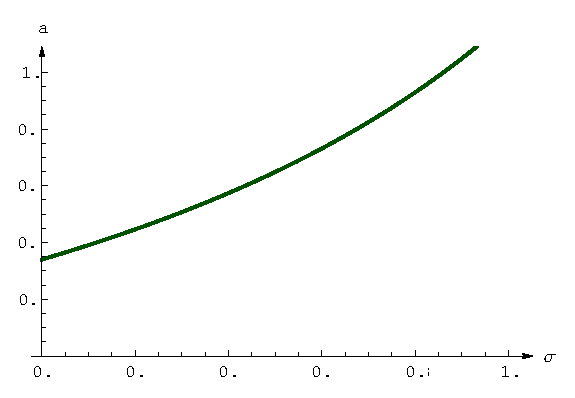
\includegraphics[width=0.47\textwidth]{images/Abbildungen/ATildeR1Ex.eps}}
%		\subfigure[Innovationsstrategie]{%
%		\centering%
%		\psfrag{a}{\small{$\widetilde{a}$}}%
%		\psfrag{0.0}[c]{\scriptsize{0}}%
%		\psfrag{0.2}[c]{\scriptsize{0.2}}%
%		\psfrag{0.4}[c]{\scriptsize{0.4}}%
%		\psfrag{0.6}[c]{\scriptsize{0.6}}%
%		\psfrag{0.8}[c]{\scriptsize{0.8}}%
%		\psfrag{1.0}[c]{\scriptsize{1}}%
%		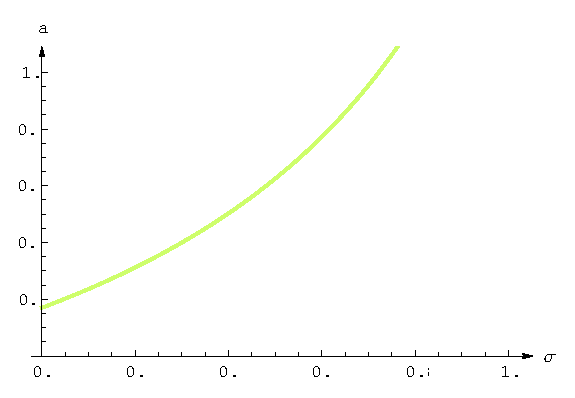
\includegraphics[width=0.47\textwidth]{images/Abbildungen/ATildeR0Ex.eps}}\\
%		\hfill\footnotesize\sffamily{\textbf{Quelle:}}  eigene Darstellung
%		\caption{$\widetilde{a}$ von der Projektgrö{\ss}e} 
%		\label{fig:aTilde}
%	\end{figure}


Die Abbildung \ref{fig:aTilde} zeigt den Zusammenhang zwischen der Nicht-Konvergenz-Falle und der Projektgrö{\ss}e $\sigma$, separat für jede Strategie. Im wesentlichen verhalten sich die Grenzwerte $\tilde{a}$ beider Strategien sehr ähnlich, da beide mit zunehmender Projektgrö{\ss}e ansteigen. Jedoch steigt der Grenzwert der \textcolor[rgb]{0.74,0.97,0.22}{Innovationsstrategie} etwas steiler an, demnach liegt die Nicht-Konvergenz-Falle bei der jeweiligen Projektgrö{\ss}e bei einem höheren Entwicklungsstand als bei der \textcolor[rgb]{0,0.32,0}{Imitationsstrategie}. Mit zunehmender Grö{\ss}e der Projekte kann die Nicht-Konvergenz-Falle durch Verwirklichung der \textcolor[rgb]{0.74,0.97,0.22}{Innovationsstrategie} verzögert werden und somit ein höherer maximal erziehlbarer Entwicklungsstand verwirklicht werden. Jedoch ist dieser Zusammenhang nicht allgemeingültig, wie die folgende Abbildung \ref{fig:beide Strategien mitaTilde} zeigt. \\


	\begin{figure*}[htbp]
		\vspace{0.13cm}
		\centering
		\psfrag{\sigma}{$\sigma$}
		\psfrag{a}{$\widetilde{a}$}
		\psfrag{0.0}[c]{\scriptsize{0}}
		\psfrag{0.2}[c]{\scriptsize{0.2}}
		\psfrag{0.4}[c]{\scriptsize{0.4}}
		\psfrag{0.6}[c]{\scriptsize{0.6}}
		\psfrag{0.8}[c]{\scriptsize{0.8}}
		\psfrag{1.0}[c]{\scriptsize{1}}
		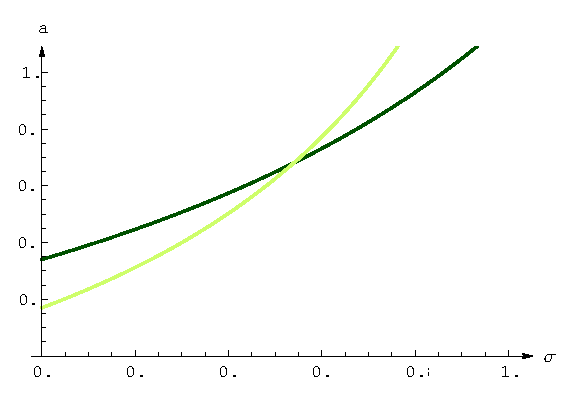
\includegraphics[width=0.7\textwidth]{images/Abbildungen/beideATildeInEinerAbbEx.eps}\\
		\hfill\footnotesize\sffamily{\textbf{Quelle:}}  eigene Darstellung
		\caption{beide Strategien mit $\widetilde{a}$}
		\label{fig:beide Strategien mitaTilde}
	\end{figure*}


Denn der Schnittpunkt beider Geraden gibt an, ab wann die \textcolor[rgb]{0.74,0.97,0.22}{Innovationsstrategie} zu einer Verzögerung der Nicht-Konvergenz-Falle beiträgt. Bis zu diesem Punkt kann durch die \textcolor[rgb]{0,0.32,0}{Imitationsstrategie} ein höherer maximaler technologischer Entwicklungsstand erreicht werden. Diese Möglichkeit ist in Abbildung \ref{fig:ein Sektor exogene WTG} dargestellt und die Volkswirtschaft erreicht den maximal erzielbaren Entwicklungsstand bevor ein Strategiewechsel bedingt durch $a_r$ ratsam wäre.\\


Der maximal erzielbare Wissensstand $\tilde{a}$ sinkt im Importsektor  und steigt im Exportsektor durch den staatlichen Eingriff an, wie aus den Abbildungen \ref{fig:exogene WTG Importsektor} und \ref{fig:exogene WTG Exportsektor} abzulesen ist. Im \textbf{Importsektor} wird dann die Nicht-Konvergenz-Falle $\tilde{a}_{Autarkie}$ nicht mehr durch die Innovation erzielt, sondern durch die \textcolor[rgb]{0,0.32,0}{Imitationsstrategie} bei $\tilde{a}_{Handel}$, da $a_{rHandel}>\tilde{a}_{Handel}$. In der Autarkiesituation lag der Grenzwert bei $a_{rAutarkie}<\tilde{a}_{rAutarkie}$, was den erfolgten Wechsel zur \textcolor[rgb]{0.74,0.97,0.22}{Innovationsstrategie} bedingt. Wohingegen im \textbf{Exportsektor} eine deutliche Verbesserung des maximal erzielbaren Wissenstandes $\tilde{a}$ durch Au{\ss}enhandel erreicht werden kann mit $\tilde{a}_{Autarkie}<\tilde{a}_{Handel}$.\\
Welche Strategie vorherrscht und die Nicht-Konvergenz-Falle eines Sektors bedingt hängt ma{\ss}geblich von der Projektgrö{\ss}e ab. Ab einer kritischen Projektgrö{\ss}e $\overline{\sigma}$ wird die Nicht-Konvergenz-Falle bei der Innovationsstrategie liegen. Dieser Wert ergibt sich aus dem Schnittpunkt beider Geraden von $\tilde{a}$ in Abbildung \ref{fig:beide Strategien mitaTilde} bzw. aus der Gleichsetzung der Gleichungen \ref{eq:aTilde1} und \ref{eq:aTilde0}.


	\begin{equation} 
		\overline{\sigma}=\frac{2+2g-\lambda\gamma}{2+2g+\lambda\gamma}
	\end{equation} 


Immer, wenn $\sigma>\overline{\sigma}$ gilt, dann fand bereits ein Wechsel bedingt durch $a_r$ statt, weil ebenfalls gilt, dass $a_r<\tilde{a}_{Imitation}$. Der maximal erzielbare Entwicklungsstand wird durch die Innovationsstrategie festgelegt. Wohingegen die Imitationsstrategie den maximalen Entwicklungsstand bildet, wenn der Grenzwert $a_r$ noch nicht überschritten wurde und somit für das Projekt gelten muss, dass $\sigma<\overline{\sigma}$.\\
Jedoch ist es durchaus denkbar, dass die Position einer Volkswirtschaft sich verändert. Im Zuge des Entwicklungsprozesses kann ein Land in stark spezialisierten Märkten Makroinnovationen entwickeln und damit den Einfluss eines technologisch gro{\ss}en Landes haben. Die Nicht-Konvergenz-Falle gibt somit nicht zwingend das finale Entwicklungspotenzial eines Landes an. 


\subsection{Wirkung von Handel auf das technologisch gro{\ss}e Land}
Eine Exportsubvention im hier beschriebenen Sinne hat auf den Abstand zur WTG eines ökonomisch gro{\ss}en Landes eindeutige gleichgerichtete Effekte. Die WTG steigt gemeinsam mit dem technischen Wissen und wird durch einen Anstieg der Projektgrö{\ss}e positiv beeinflusst. Die WTG verhält sich somit endogen.  
Anhand der Abbildungen \ref{fig:endogene WTG Importsektor} und \ref{fig:endogene WTG Exportsektor} lassen sich die Reaktionen der Sektoren auf die handelspolitische Ma{\ss}nahme verdeutlichen.\\


	\begin{figure}[htb]
		\vspace{0.13cm}
		\centering 
		\psfrag{a}{$a$}
		\psfrag{t}{  $_t$}
		\psfrag{-}{  $_-$}
		\psfrag{1}{\, $_1$}
		\psfrag{0.0}[c]{\scriptsize{0}}
		\psfrag{0.2}[c]{\scriptsize{0.2}}
		\psfrag{0.4}[c]{\scriptsize{0.4}}
		\psfrag{0.6}[c]{\scriptsize{0.6}}
		\psfrag{0.8}[c]{\scriptsize{}}
		\psfrag{1.0}[c]{\scriptsize{1}}
		\begin{overpic}
			[width=0.9\textwidth]{images/Abbildungen/ImEndogeneWTG.eps}
			\put(73.2,0.5){\textcolor{black}{$\hat{a}_{tAutarkie}$}}
			\put(23,0.7){\textcolor{black}{$a_{rAutarkie}$}}
			\put(60.3,0.7){\textcolor{black}{$a_{rHandel}$}}
			\put(-0.4,45.5){\textcolor{black}{\scriptsize{0.8}}}
			\put(92,0.5){\textcolor{black}{\scriptsize{1}}}
		\end{overpic}\\
		\hfill\footnotesize\sffamily{\textbf{Quelle:}}  eigene Darstellung
		\caption{endogene WTG im Importsektor}
		\label{fig:endogene WTG Importsektor}
	\end{figure}


Beginnend mit dem \textbf{Importsektor} aus Abbildung \ref{fig:endogene WTG Importsektor} führt die Exportsubvention zu verhältnismä{\ss}ig kleineren Projekte im Vergleich zur Autarkiesituation. Insgesamt kann sich der Wissenszuwachs des Importsektors erhöhen indem die \textcolor[rgb]{0,0.32,0}{Imitationsstrategie} verfolgt wird. Die \textcolor[rgb]{0.74,0.97,0.22}{Innovationsstrategie} würde nun zu einem geringeren Entwicklungsstand führen, was wiederum eindeutig zeigt, dass der Importsektor seinen Schwerpunkt auf langfristige Beziehungen, die Ausdruck der \textcolor[rgb]{0,0.32,0}{Investitionsstrategie} sind, legen sollte. Die Grenzwerte $a_r$ und $\hat{a}_t$ steigen beide mit sinkender Projektgrö{\ss}e und deuten an, dass sowohl hinsichtlich der Produktivität $\hat{a}_{tHandel}>1$ als auch der Wirtschaftlichkeit $a_{rHandel}>a_{rAutarkie}$ ein späterer Wechsel zur \textcolor[rgb]{0.74,0.97,0.22}{Innovationsstrategie} zu empfehlen ist. Der Sektor ist vornehmlich durch die \textcolor[rgb]{0,0.32,0}{Imitationsstrategie} geprägt. Die kleinen Importprojekte verlieren bei der strategischen Planung zunehmend an Bedeutung, da die unternehmerischen Umsätze durch die sehr kleinen Projekte verglichen mit den gesamtwirtschaftlichen Umsätzen nur einen relativ geringen Anteil betragen. Bleibt die Angestelltenstruktur gemä{\ss} der \textcolor[rgb]{0,0.32,0}{Imitationsstrategie} unverändert, dann liegt der Schwerpunkt bei den gro{\ss}en Projekten, die durch die weniger gut ausgebildeten erfahrenen Ingenieure ermöglicht werden.\\ Interessant ist ein Vergleich von Volkswirtschaften deren Entwicklungsstand nur geringfügig grö{\ss}er oder kleiner als $a_{rHandel}$ ist. Da je nach Startsituation das relativ weiter entwickelte Land mit $a_{t-1}>a_{rHandel}$ von dem weniger weit entwickelten Land $a_{t-1}<a_{rHandel}$ durch den Wechsel zur \textcolor[rgb]{0.74,0.97,0.22}{Innovationsstrategie} überholt werden kann.\\


	\begin{figure}[htb]
		\vspace{0.13cm}
		\centering 
		\psfrag{a}{$a$}
		\psfrag{t}{  $_t$}
		\psfrag{-}{  $_-$}
		\psfrag{1}{\, $_1$}
		\psfrag{0.0}[c]{\scriptsize{0}}
		\psfrag{0.2}[c]{\scriptsize{}}
		\psfrag{0.4}[c]{\scriptsize{0.4}}
		\psfrag{0.6}[c]{\scriptsize{0.6}}
		\psfrag{0.8}[c]{\scriptsize{}}
		\psfrag{1.0}[c]{\scriptsize{1}}
		\begin{overpic}
			[width=0.9\textwidth]{images/Abbildungen/ExEndogeneWTG.eps}
			\put(25,0.5){\textcolor{black}{$\hat{a}_{tHandel}$}}
			\put(71.6,0.5){\textcolor{black}{$\hat{a}_{tAutarkie}$}}
			\put(22.4,-1.6){\textcolor{black}{$a_{rAutarkie}$}}
			\put(-0.73,13.3){\textcolor{black}{\scriptsize{0.2}}}
			\put(-0.73,45){\textcolor{black}{\scriptsize{0.8}}}
		\end{overpic}\\
		\hfill\footnotesize\sffamily{\textbf{Quelle:}}  eigene Darstellung
		\caption{endogene WTG im Exportsektor}
		\label{fig:endogene WTG Exportsektor}
	\end{figure}


Im \textbf{Exportsektor} in Abbildung \ref{fig:endogene WTG Exportsektor} verhält es sich etwas anders. Grundsätzlich führt eine grö{\ss}ere Projektgrö{\ss}e zu einem höheren Wissenszuwachs durch die \textcolor[rgb]{0.74,0.97,0.22}{Innovationsstrategie} und zu einer Wissensreduktion, sollte sich der Sektor nach der \textcolor[rgb]{0,0.32,0}{Investitionsstrategie} ausrichten. Auch im Exportsektor hängt die Wahl der Strategie vom Entwicklungsstand eines Landes ab. Für weniger weit entwickelte Länder ist die \textcolor[rgb]{0,0.32,0}{Imitationsstrategie} noch immer produktiver als die \textcolor[rgb]{0.74,0.97,0.22}{Innovationsstrategie}, jedoch führt sie zu einem geringeren Wissenszuwachs als dies \dashuline{ohne Handelspolitik} möglich wäre. Bei der endogenen WTG führt die \uline{Exportsubvention} allgemein zu einer relativ schlechteren Produktivität. Der Entwicklungspfad eines Landes wird nicht uneingeschränkt von der staatlichen Unterstützung beschleunigt, jedoch werden die Innovationen in diesem Sektor gefördert und ein früherer Wechsel zur \textcolor[rgb]{0.74,0.97,0.22}{Innovationsstrategie} ist sinnvoll. Die Exportförderung wirkt ähnlich wie eine Förderung von Unternehmensgründungen, da diese sofern sie sich im Exportsektor ansiedeln, eine solidere und sicherere Ausgangssituation vorfinden, als ohne unterstützende Ma{\ss}nahmen.\\


Werden wieder die Schwellenwerte $a_r$ und $\hat{a}_t$ hinzugezogen, dann sinken beide Werte mit steigender Projektgrö{\ss}e. Da hier $a_{rHandel}<0$ gilt, ist es ökonomisch sinnvoll nur noch die \textcolor[rgb]{0.74,0.97,0.22}{Innovationsstrategie} zu verfolgen. Durch die Exportsubvention stellen sich nur Länder mit einem Entwicklungsstand $a_{t-1}>a_{rAutarkie}$ besser.\\


Die Nicht-Konvergenz-Falle $\tilde{a}$ ist auch bei Handel bei der endogenen WTG nicht relevant, da alle Volkswirtschaften sich im Entwicklungsprozess zur Innovationsstrategie ausrichten und dann zur WTG mit $\tilde{a}=1$ konvergieren. 


\section{Zwischenfazit}
Das vorliegende Wachstumsmodell zeigt, inwiefern  Handel die technische Entwicklung eines Landes fördert. Um die Ergebnisse zu verdeutlichen, wurde eine handelsfördernde Ma{\ss}nahme eingeführt und es lassen sich Entwicklungsstrategien für verschiedene Entwicklungsphasen zuordnen. Neben dem Entwicklungsstand eines Landes wurde auch die Bedeutung einer Innovation für das Land miteinbezogen.\\
Zusammenfassend lässt sich festhalten, dass ökonomisch und technologisch kleine Länder bei einer exogenen WTG von einer Exportförderung profitieren. Im Exportsektor kann es zu einer deutlichen Verbesserung des technischen Entwicklungsstandes kommen und der Abstand zur WTG mindert sich eher, als dies ohne Exportförderung möglich ist, unabhängig von dem technologischen Entwicklungsstand eines Landes.\footnote{Siehe dazu auch Abbildung \ref{fig:exogene WTG Exportsektor}.} Es findet eine eindeutige Verlagerung des Schwerpunktes dieses Sektors zur Innovationsstrategie statt. Wohingegen der Importsektor sich ausschlie{\ss}lich auf die Imitationsstrategie konzentriert. Dabei stellen sich relativ wenig entwickelte Länder sowie auch deutlich weiter entwickelte Länder mit der Exportsubvention schlechter und sollten auf Au{\ss}enhandel in diesem Sektor zunächst verzichten. In diesem, hier angenommenen, Fall profitiert der Importsektor nur in wenigen Fällen vom Au{\ss}enhandel. Demnach verschlechtert sich das allgemeine Entwicklungspotential $\tilde{a}$ dieses Sektors durch Handel. Jedoch kann insgesamt von einer Verbesserung durch Handel ausgegangen werden.\\


	\begin{figure}[h!] 
		\vspace{0.13cm}
		\centering 
		\psfrag{a}{$a$}
		\psfrag{t}{  $_t$}
		\psfrag{-}{  $_-$}
		\psfrag{1}{\, $_1$}
		\psfrag{0.0}[c]{\scriptsize{0}}
		\psfrag{0.2}[c]{\scriptsize{0.2}}
		\psfrag{0.4}[c]{\scriptsize{}}
		\psfrag{0.6}[c]{\scriptsize{0.6}}
		\psfrag{0.8}[c]{\scriptsize{0.8}}
		\psfrag{1.0}[c]{\scriptsize{1}}
		\begin{overpic}	[width=0.9\textwidth]{images/Abbildungen/beideSektorenExoWTG.eps}
			\put(35.9,0.7){\color[rgb]{0,0.32,0}{$\tilde{a}_{Im}$}}
			\put(59.2,0.7){\color[rgb]{0.74,0.97,0.22}{$\tilde{a}_{Ex}$}}
			\put(-0.73,24.2){\textcolor{black}{\scriptsize{0.4}}}
		\end{overpic}\\
		\hfill\footnotesize\sffamily{\textbf{Quelle:}}  eigene Darstellung
		\caption{beide Sektoren bei exogener Welttechnologiegrenze}
		\label{fig:beide Sektor exogene WTG}
	\end{figure}


Die gemeinsame Darstellung des Import- mit dem Exportsektor in Abbildung \ref{fig:beide Sektor exogene WTG}\footnote{In der Abbildung sind die Strategien des Exportsektors mit den dickeren Linien gekennzeichnet und die Strategien des Importsektor mit den dünneren Linien.}  zeigt, dass eine Exportförderung in einem technologisch kleinen Land zu einer Konzentration des Importsektors auf die Imitationsstrategie und des Exportsektors auf die Innovationsstrategie führt, unabhängig vom Entwicklungsstand des Landes.Der Vergleich beider Sektoren zeigt eindeutig, dass die Nicht-Konvergenz-Falle im Exportsektor $\tilde{a}_{Ex}$ deutlich später eintritt, als im Importsektor $\tilde{a}_{Im}$ und somit auch einen höheren maximal erzielbaren technologischen Entwicklungsstand erreichen kann, da $\tilde{a}_{Im}<\tilde{a}_{Ex}$ gilt. Die lokale Technologiegrenze wird hier demzufolge eindeutig durch den Exportsektor gebildet und das Land profitiert insgesamt vom Au{\ss}enhandel.\\ 


Bei einer endogenen WTG hingegen verschlechtert sich das Entwicklungspotenzial des Exportsektors teilweise. Unabhängig von dem Entwicklungsstand des Landes wird die Innovationsstrategie verfolgt. Erst ab dem bestimmten technologischen Entwicklungsniveau $a_{rAutarkie}$ stellt sich eine Volkswirtschaft mit einer Exportförderung besser als bei Autarkie.\footnote{Dieser Zusammenhang ist der Abbildung \ref{fig:endogene WTG Exportsektor} zu entnehmen.} Demzufolge sollte sich bis zu diesem Entwicklungsstand die Volkswirtschaft nicht für Handel öffnen, sofern nur der Exportsektor betrachtet wird. Denn der Zuwachs des gesamtwirtschaftlichen technischen Wissens bestimmt sich durch die vorherrschende Imitationsstrategie im Importsektor. In diesem Sektor sollte jedoch wieder differenziert werden hinsichtlich des Entwicklungsstandes und der Öffnung für Au{\ss}enhandel. Sofern ein Land recht weit entwickelt ist und den Grenzwert $a_{rHandel}$ bereits überschritten hat verschlechtern sich die Entwicklungsmöglichkeiten im Importsektor. Letztlich verbessert sich die gesamte Volkswirtschaft durch Au{\ss}enhandel, im endogenen Fall jedoch ist dies grö{\ss}tenteils auf den Importsektor zurückzuführen.\footnote{Zu finden sind diese Grenzwerte in Abbildung \ref{fig:endogene WTG}} 
		
			
	\begin{figure}[h!] 
		\vspace{0.13cm}
		\centering  
		\psfrag{a}{$a$}
		\psfrag{t}{  $_t$}
		\psfrag{-}{  $_-$}
		\psfrag{1}{\, $_1$}
		\psfrag{0.0}[c]{\scriptsize{0}}
		\psfrag{0.2}[c]{\scriptsize{0.2}}
		\psfrag{0.4}[c]{\scriptsize{0.4}}
		\psfrag{0.6}[c]{\scriptsize{0.6}}
		\psfrag{0.8}[c]{\scriptsize{0.8}}
		\psfrag{1.0}[c]{\scriptsize{1}}
		\begin{overpic}[width=0.9\textwidth]{images/Abbildungen/beide.eps}
			\put(58.2,0.9){\textcolor{black}{$a_{rIm}$}}
		\end{overpic}\\
		\hfill\footnotesize\sffamily{\textbf{Quelle:}}  eigene Darstellung
		\caption{beide Sektoren bei endogener Welttechnologiegrenze}
		\label{fig:beideSektorenendogeneWTG}
	\end{figure}


In der zweiten sektorübergreifenden Darstellung \ref{fig:beideSektorenendogeneWTG}\footnote{Auch hier können die Sektoren wieder anhand der Dicke der Linien unterschieden werden: Die Strategien des Exportsektors sind mit den dickeren Linien gekennzeichnet und die Strategien des Importsektor mit den dünneren Linien.} liegt der Schwerpunkt des Exportsektors ebenfalls in der Innovationsstrategie, wohingegen beim Importsektor ab einem bestimmten technologischen Entwicklungsstand von $a_{rIm}$ die weniger produktive Innovationsstrategie gewählt wird. Bis zu diesem Schwellenwert bildet der Importsektor den lokalen technologischen Wissensstand der Volkswirtschaft ab und bedingt dadurch stärker den technischen Fortschritt als der innovierende Exportsektor.\newline 
Zusammenfassend lässt sich feststellen, dass in technologisch kleinen Ländern unabhängig von dem Entwicklungsstand im Importsektor die Imitationsstrategie und im Exportsektor die Innovationsstrategie verfolgt wird. Es stellen sich Länder aller Entwicklungsstufen besser durch eine Exportsubvention. In technologisch gro{\ss}en Ländern profitieren ebenfalls alle Länder, unabhängig vom technologischen Entwicklungsstand, von der Förderung des Exportsektors. 


\chapter{Kombination beider Modellvarianten}\label{Kombi}
Anhand der bisherigen Ergebnisse konnte festgestellt werden, dass sich die Entscheidung
der Haushalte zwischen der eigenen Bildung oder der Erwerbstätigkeit durch die Integration vom Au{\ss}enhandel zugunsten der Weiterbildung verlagerte. Hebt man dieses Ergebnis auf die makroökonomische Ebene, dann kann insgesamt von einer besser ausgebildeten Gesellschaft ausgegangen werden. Die Öffnung eines Landes führt dazu, dass mehr Humankapitel akkumuliert wird. Dieses zusätzliche Humankapital kann nun verwendet werden, um den technischen Fortschritt durch Imitation oder Innovation in einem Land zu steigern. Das zuvor behandelte Modell in Kapitel \ref{Papier2} stellt somit den notwendigen vorgelagerten Prozess dar, durch den es erst möglich wird den technischen Entwicklungsstand eines Landes zu verbessern, was in Kapitel \ref{Papier1} umfasend analysiert wurde.\newline 
Das folgende Kapitel soll nun die Wahrscheinlichkeit einer guten Ausbildung eines Ingenieurs $\lambda$ genauer betrachten.\footnote{Dabei wird nun, ohne Verlust von Allgemeinheit, von einer exogenen Projektgrö{\ss}e ausgegangen.} Durch den gezeigten positiven Zusammenhang von Au{\ss}enhandel und Investitionen in Bildung steigt nun ebenfalls die Wahrscheinlichkeit, dass ein Ingenieur mit hohen technischen Fähigkeiten ausgestattet ist, denn ein grundlegend angepasstes und in diesem Fall verbessertes Bildungssystem führt zu einer besser ausgebildeten Bevölkerung. Somit steigt in diesem Fall auch die Wahrscheinlichkeit einen gut ausgebildeten Ingenieur einzustellen an, als dies ohne Handel der Fall wäre.  \\
Ohne, dass der Handel explizit politisch unterstützt wurde, verbessert sich der technologische Entwicklungsstand eines Landes. Auch dies ist wieder abhängig von der strategischen Entscheidung eines Unternehmens bzw. der Volkswirtschaft. Die folgende Abbildung \ref{lambdaExo} stellt den Vergleich der beiden Strategien einer geöffneten und einer geschlossenen Volkswirtschaft dar.\\


	\begin{figure}[htbp] 
		\vspace{0.13cm}
		\centering  
		\psfrag{a}{$a$}
		\psfrag{t}{  $_t$}
		\psfrag{-}{  $_-$}
		\psfrag{1}{\, $_1$}
		\psfrag{0.0}[c]{\scriptsize{0}}
		\psfrag{0.2}[c]{\scriptsize{0.2}}
		\psfrag{0.4}[c]{\scriptsize{0.4}}
		\psfrag{0.6}[c]{\scriptsize{0.6}}
		\psfrag{0.8}[c]{\scriptsize{0.8}}
		\psfrag{1.0}[c]{\scriptsize{1}}
		\begin{overpic}[width=0.9\textwidth]{images/Abbildungen/Lambdaaexo.eps}
			\put(47,-0.93){\textcolor{black}{$\hat{a}_{t\textit{Handel}}$}}
			\put(74.5,-0.86){\textcolor{black}{$\hat{a}_{t\textit{Autarkie}}$}}
			\put(14.3,-1.1){\textcolor{black}{$a_{rHandel}$}}
			\put(21.7,0.5){\textcolor{black}{$a_{rAutarkie}$}}
		\end{overpic}\\
		\hfill\footnotesize\sffamily{\textbf{Quelle:}}  eigene Darstellung
		\caption{Einfluss der Wahrscheinlichkeit für qualifizierte Arbeit $\lambda$ bei exogener WTG auf den technologischen Entwicklungsstand}
		\floatfoot{- Anstieg der Wahrscheinlichkeit für qualifizierte Arbeit $\lambda$ von 50\% auf 80\% durch Freihandel -}
		\label{lambdaExo}
	\end{figure}


Von einer geschlossenen Volkswirtschaft ausgehend, die weitestgehend autark ist, steigt in dem hier dargestellten Fall die Wahrscheinlichkeit einen Ingenieur eingestellt zu haben, der hohe technische Fähigkeiten besitzt von 50\% auf 80\% an. Füt den technologischen Entwickungsstand eines Landes bedeutet dies, dass hierdurch ein höherer zukünftiger Zustand erreicht werden kann, für jeden technologischen Entwicklungsstand eines Landes. Die Geraden verlaufen steiler und dementsprechend führt dies unabhängig von der Strategiewahl zu einem zusätzlichen Wachstum, denn je besser ausgebildet die Arbeiter sind, desto mehr Wissen kann transferiert werden und die entsprechenden Volkswirtschaften profitieren durch diese Wissens-Spillover-Effekte.\\ 
Der Grenzwert $\hat{a}$ betrachtet den Strategiewechsel losgelöst von möglichen Kosten und sinkt mit zunehmendem Handel. Auf die Entwicklung eines Landes bezogen wird nun schon für Länder mit einem geringeren technologischem Entwicklungsstand der Wechsel zur \textcolor[rgb]{0.74,0.97,0.22}{Innovationsstrategie} empfohlen, da diese produktiver ist. In einer \dashuline{geschlossenen Volkswirtschaft}, in der von einem geringeren Kapitalstock ausgegangen werden kann, dominierte die \textcolor[rgb]{0,0.32,0}{Imitationsstrategie}. Mit der \underline{Öffnung des Landes} resultiert grundsätzlich ein deutlich höherer technologischer Entwicklungsstand, der zunächst eher durch die \textcolor[rgb]{0,0.32,0}{Imitationsstrategie} erzielt werden kann.  Der höhere Entwicklungsstand ergibt sich durch besser ausgebildete Arbeiter, die nun vorhanden sind. Für innovierende Tätigkeiten sind hohe technische Fähigkeiten notwendig, die fortan eingesetzt werden können und die Innovationsrate steigern.\\
Berücksichtigt man die Gewinnaussichten der Unternehmer, dann zeigt auch der Grenzwert $a_r$, dass Offenheit zu einem früheren Wechsel zur Innovationsstrategie führt. \\


	\begin{figure*}[h]
		\vspace{0.13cm}
		\centering
		\psfrag{a}{$a_r$}
		\psfrag{t}{}
		\psfrag{-}{-}
		\psfrag{1}{1}
		%\psfrag{-0.2}[c]{\scriptsize{}}
		%\psfrag{-0.4}[c]{\scriptsize{}}
		\psfrag{0.0}[c]{\scriptsize{0}}
		\psfrag{0.2}[r]{\scriptsize{0.2}}
		\psfrag{0.4}[r]{\scriptsize{0.4}}
		\psfrag{0.6}[r]{\scriptsize{0.6}}
		\psfrag{0.8}[r]{\scriptsize{0.8}}
		\psfrag{1.0}[r]{\scriptsize{1}}
		\psfrag{L}[c]{$\lambda$}
		\begin{overpic}[width=0.5\textwidth]{images/Abbildungen/aRLambda.eps}
			%\put(98,16){\textcolor{black}{$\sigma$}}
			%\put(0.5,23){\textcolor{black}{\scriptsize{0.2}}}
			%\put(0.5,30){\textcolor{black}{\scriptsize{0.4}}}
			%\put(0.5,38){\textcolor{black}{\scriptsize{0.6}}}
			%\put(0.5,45.1){\textcolor{black}{\scriptsize{0.8}}}
			
			%\put(20.6,12){\textcolor{black}{\scriptsize{0.2}}}
			%\put(38.4,12){\textcolor{black}{\scriptsize{0.4}}}
			%\put(56.2,12){\textcolor{black}{\scriptsize{0.6}}}
			%\put(74.3,12){\textcolor{black}{\scriptsize{0.8}}}
		\end{overpic}\\
		\hfill\footnotesize\sffamily{\textbf{Quelle:}}  eigene Darstellung
		\caption{$a_r$ in Abhängigkeit von $\lambda$ }
		\label{fig:VerhaltenAR}
	\end{figure*}


Sofern die Wahrscheinlichkeit ansteigt, dass ein junger Ingenieur hohe technische Fähigkeiten besitzen könnte, werden diese Möglichkeiten von den Unternehmen erkannt und es findet ein früherer Wechsel der Strategie statt, da ein geringerer Wert von $a_r$ folgt. Kurze berufliche Beziehungen werden präferiert und ältere  weniger qualifizierte Ingenieure ausgetauscht, wodurch die Kosten reduziert werden. Dieses Modell zeigt direkt, dass Ineffizienzen beseitigt bzw. gemindert werden, indem das Risiko eingegangen wird junge Ingenieure einzustellen, die möglicherweise höher qualifiziert sind.
In diesem Zusammenhang führt Handel zu tendenziell mehr Entlassungen weniger qualifizierter Ingenieure und zu einem Anstieg der Innovationsrate.\\
Anzumerken ist an dieser Stelle, dass bei relativ weiter entwickelten Volkswirtschaften, die in Relation zur WTG mit mindestens 80\% entwickelt sind, beide Strategien in Abbildung \ref{fig:beideSektorenendogeneWTG} nicht definiert sind. Bei diesen Ländern kann davon ausgegangen werden, dass sie nach dem Wechsel zur Innovationsstrategie keine Mikro- sondern Makroinnovationen entwickeln und somit als technologisch gro{\ss}es Land selbst die WTG dieser Branche stellen. Dann handelt es sich um eine endogene WTG, die in der folgenden Abbildung \ref{lambdaEndo} dargestellt ist.\\


	\begin{figure}[htbp] 
		\vspace{0.13cm}
		\centering  
		\psfrag{a}{$a$}
		\psfrag{t}{  $_t$}
		\psfrag{-}{  $_-$}
		\psfrag{1}{\, $_1$}
		\psfrag{0.0}[c]{\scriptsize{0}}
		\psfrag{0.2}[c]{\scriptsize{0.2}}
		\psfrag{0.4}[c]{\scriptsize{0.4}}
		\psfrag{0.6}[c]{\scriptsize{0.6}}
		\psfrag{0.8}[c]{\scriptsize{}}
		\psfrag{1.0}[c]{\scriptsize{1}}
		\begin{overpic}[width=0.9\textwidth]{images/Abbildungen/Lambdaaendo.eps}
			\put(44.5,0.7){\textcolor{black}{$\hat{a}_{t\textit{Handel}}$}}
			\put(73,0.7){\textcolor{black}{$\hat{a}_{t\textit{Autarkie}}$}}
			\put(-1,45.5){\textcolor{black}{\scriptsize{0.8}}}
			%\put(-0.5,55.5){\textcolor{black}{\scriptsize{1}}}
			\put(13,-1){\textcolor{black}{$a_{rHandel}$}}
			\put(21.5,0.7){\textcolor{black}{$a_{rAutarkie}$}}
		\end{overpic}\\
		\vspace{0.3cm}
		\hfill\footnotesize\sffamily{\textbf{Quelle:}}  eigene Darstellung
		\caption{Einfluss der Wahrscheinlichkeit für qualifizierte Arbeit $\lambda$ bei endogener WTG auf den technologischen Entwicklungsstand}
		\floatfoot{- Anstieg der Wahrscheinlichkeit für qualifizierte Arbeit $\lambda$ von 50\% auf 80\% durch Freihandel -}
		\label{lambdaEndo}
	\end{figure}


Auch hier wird von einer staatlichen Exportförderung abstrahiert und einzig der Effekt des Au{\ss}enhandels durch höhere Bildung auf den Entwicklungsstand eines Landes betrachtet. In einem technologisch gro{\ss}en Land weitet sich die WTG mit jeder zusätzlichen Innovation aus.\\ Ist dieses Land \underline{offen}, dann entsteht zunächst der Eindruck, dass es seinen direkten Wissensvorsprung gegenüber der übrigen Welt verliert. Abbildung \ref{lambdaEndo} stellt dar, dass sich der technologische Entwicklungsstand eines Landes durch Au{\ss}enhandel, unabhängig von dem anfänglichen Entwicklungsstand verschlechtert. Dieser Anschein wird durch die relative Darstellung des Entwicklungsstandes hervorgerufen.\footnote{Dies ergibt sich durch die Definition des Abstands zur Welttechnologiegrenze eines Landes $a_t$ als $A_t/\bar{A_t}$.} Der Entwicklungsstand eines Landes steigt bei einer endogenen WTG nur dann an, wenn es selbst einen stärkeren technologischen Wissenszuwachs generiert, als das Land, welches die Technologiegrenze erweitert hat. Dass hierdurch Au{\ss}enhandel die Wahrscheinlichkeit steigt qualifizierte Arbeitskräfte einzustellen, steigert die Produktivität eines Landes und führt zu Wachstum. Jedoch ist die Produktivität des Landes der WTG noch immer höher und die Ausweitung der WTG ist stärker als die Minderung des Abstandes. Diese Argumentation kann auch anhand der in Kapitel \ref{Efekkte} diskutieren Effekte gestützt werden. Es wurde gezeigt, dass Handel zu einem Produktivitätszuwachs durch den Marktgrö{\ss}eneffekt, den Wettbewerbseffekt und den Wissens-Spillover-Effekt führt. Dieser positiv wirkende Effizienzeffekt wird hier durch den negativ wirkenden Wachstumseffekt dominiert. Der Wachstumseffekt spiegelt das Wachstum der WTG wieder, das den relativen Abstand ausweitet.\footnote{Der Wachstumseffekt resultiert aus der Endogenität der WTG und muss somit nur im endogenen Fall untersucht werden. Bei einer exogenen WTG ist demzufolge immer der Effizienzeffekt dominant.} In der hier dargestellten Situation profitieren vom Au{\ss}enhandel sowohl Unternehmen, die, die \textcolor[rgb]{0.74,0.97,0.22}{Innovationsstrategie} nutzen, als auch die die die \textcolor[rgb]{0,0.32,0}{Imitationsstrategie} verfolgen, jedoch profitiert das Land der WTG stärker, so dass der technologische Entwicklungsstand sinkt, der relativ zur WTG bemessen wird. Das führt dazu, dass ein technologisch gro{\ss}es Land sich relativ gesehen langsamer entwickelt. Dies kann beispielsweise daran liegen, dass auch das Land der WTG von den Ressourcen, wie Kapital, Arbeit und getätigten Investitionen gleicherma{\ss}en profitiert, wie das Ursprungsland, welches darüber hinaus noch Wissen generiert.\\
Nachdem nun die Aussagekraft der Abbildung interpretiert wurde, lässt sich ein optimaler Entwicklungspfad ableiten. Auch hier steigen die Innovationsanreize und es findet aufgrund der besseren Humankapitalausstattung ein früherer Wechsel zur \textcolor[rgb]{0.74,0.97,0.22}{Innovationsstrategie} statt. Jedoch ist der zukünftige Abstand zur WTG höher als in der \dashuline{Autarkiesituation}. Dieser Wechsel wird sowohl durch einen kleineren Grenzwert von $\hat{a}$ als auch von $a_r$ angezeigt.
\bigskip


Zusammenfassend lässt sich feststellen, dass Volkswirtschaften stärker von der Imitationsstrategie profitieren, sofern ihre Mikroinnovationen die WTG nicht tangieren. Erst mit zunehmender Bedeutung der Innovationen folgen die Länder der Innovationsstrategie, die den technologischen Entwicklungsprozess fördert, auch wenn der relative Abstand zur WTG dabei nicht sinkt. \\
Somit wird in dieser Arbeit das tatsächliche Verhalten vieler Länder wiedergespiegelt, die ihren Schwerpunkt auf die Imitation legen. Nur wenige sehr weit entwickelte Länder fokussieren sich auf Innovationen. Viele von ihnen sind meist auch technologisch gro{\ss} und somit führend in ihrer Branche. Durch Au{\ss}enhandel kann insgesamt ein höheres Niveau an Bildung erreicht werden. Demzufolge wird nicht nur besser und mehr innoviert, sondern auch imitiert.
%%\documentclass[12pt]{article}
%\usepackage[latin1]{inputenc}% erm\"oglich die direkte Eingabe der Umlaute 
%\usepackage[T1]{fontenc} % das Trennen der Umlaute
%\usepackage{ngerman}
%\usepackage{a4wide}
%\usepackage{color}
%\usepackage{amsmath} % braucht man um die gleichungen zu labeln und zu zitieren
%\usepackage{lmodern,amssymb,xcolor}

%\begin{document}
%\renewcommand{\baselinestretch}{1.35}\normalsize
%\chapter{\textcolor[rgb]{0.8,0.6,1}{Modell Lucas/Neuen NAMEN f�r Modell}}\label{ModellLucas}
\chapter{Erwerbst�tigkeit vs. Bildung - \newline
Die Wirkung des Freihandels auf die Humankapitalakkumulation eines Landes}
\chaptermark{Erwerbst�tigkeit vs. Bildung}\label{Papier2}
\section{Intuition}

Humankapital und Sachkapital wird in Modellen h�ufig unter dem allgemeinen Begriff des Kapitals zusammengefasst.\footnote{Wie es beispielsweise im AK-Modell angenommen wird \cite{Rebelo.1991}.} Jedoch unterscheiden sich beide Kapitalarten deutlich hinsichtlich ihrer Wachstumswirkung, Herstellung und Abschreibung \cite{Ortigueira.1997}.\\
Dies zeigen auch Beispiele des letzten Jahrhunderts vor allem in Asien. In relativ kurzer Zeit wurden durch Investitionen in Kapital h{\"o}here Wachstumsraten erzielt worauf jedoch wirtschaftliche Krisen folgten. Der Grund f{\"u}r die zunehmenden Probleme lag unter anderem darin, dass zwar grunds{\"a}tzlich mehr Produktionsfaktoren in den Industriesektor investiert wurden, sich dadurch aber nicht die Produktivit{\"a}t erh{\"o}ht hat. Der Ausbau des Bildungssektors und die damit einhergehenden Investitionen in Humankaptial wurden  vernachl{\"a}ssigt, was den Mangel qualifizierter Arbeit und das Ausbleiben technologischer Neuerungen bedingte. Die effektivere Entwicklungsstrategie asiatischer L{\"a}nder k{\"o}nnte nun darin bestehen den gleichzeitigen Ausbau des Bildungssektors zu f{\"o}rdern und Technologien indirekt zu importieren, um drohenden Krisen entgegenzuwirken \citep{Krugman.2015}. \newline
Dieser indirekte Import birgt die Idee der globalen Wissensdiffusion durch Freihandel und der globalen Integration einer Volkswirtschaft. Beispielhaft f�r die Entwicklungsf�rderung durch den Wissenstransfer sind die ehemaligen Kolonien, die beispielsweise von kolonisatorisch implementierten Institutionen profitierten. Au{\ss}erdem konnte das technische Wissen sowie F�higkeiten der Kolonialm�chte �bernommen werden. Dieser Humankapitaltransfer f�hrte dazu, dass einige Volkswirtschaften wie �gypten oder S�dafrika heute weiter entwickelt sind als direkte Nachbarn mit �hnlichen Ausgangsbedingungen wie Libyen oder Mosambik \citep{Acemoglu.2000b}.\\
Auch das Beispiel der Pharmaindustrie soll die M�glichkeiten internationalen Wissenstransfers verdeutlichen. Werden in relativ weit entwickelten L�ndern Medikamente, wie beispielsweise Impfstoffe durch vorwiegend gentechnische Verfahren in Bakterienkulturen hergestellt, deren Produktion somit sehr humankapitalintensiv ist, so ist der Prozess in weniger weit entwickelten L�ndern zur Produktion dieser Impfstoffe noch durch traditionelle Verfahren gepr�gt.\footnote{Hier werden biochemische Prozesse im Labor nicht k�nstlich hervorgerufen, sondern Resistenzen direkt bei vorher infizierten Tieren gewonnen. Die anschlie{\ss}end isolierten Antik�rpern k�nnen auf den Menschen �bertragen werden \citep{Aberle.2010}.} Dieses Beispiel zeigt unterschiedliche Verfahrensm�glichkeiten verschiedener Entwicklungsstadien von Volkswirtschaften auf, und, dass ein Import des Impfstoffes einerseits die Ressourcen des Landes langfristig schonen w�rde sowie direkt zu einem Wissenstransfer f�hrt, der eine m�gliche Imitation des Gutes grunds�tzlich nicht ausschlie{\ss}t. Unabh�ngig von dem Import der G�ter ist f�r die Imitation die Qualifikation und somit die Bildung der Bev�lkerung notwendig, um diesen Wissenstransfer umfassend ausnutzen zu k�nnen. \\
Diesem kausalen Zusammenhang folgend, soll gezeigt werden, dass sich ein Land durch den Import von Humankapital besser stellt,  ohne dabei jedoch Migration in die Modellwelt zu integrieren. Koppelt man den Ideenfluss zwischen zwei L{\"a}ndern, der auch als Wissensfluss interpretiert werden kann, an den G{\"u}terfluss, dann wird indirekt Humankapital importiert \citep{RiveraBatiz.1991a}.\\
Der Kerngedanke ist, dass das Wachstum eines weniger weit entwickelten Landes ansteigt, wenn G�ter importiert werden, die mit relativ viel Humankapital produziert wurden. Es folgt ein langfristiger Effekt bez�glich der Ressourcen durch Faktormehrung im Bildungssektor. Denn je mehr von diesem Gut importiert wird, desto weniger muss davon im Land selbst produziert werden und es kann dadurch die Produktionsfaktoren umverteilen. In der folgenden Modellwelt bedeutet dies, dass nun das eingesparte Humankapital die Humankapitalakkumulation f�rdert. Jedoch f�hrt ein Import von humankapitalintensiv produzierten G�tern auch zu einem kurzfristigen Effekt des einmaligen Wissenstransfers. Mit dem Gut wird ebenso technisches Wissen transferiert und f�hrt zu einem Erkenntnisgewinn. Technologien, Verfahren und Einsatzfaktoren k�nnen analysiert werden, um diese zu einem sp�teren Zeitpunkt zu imitieren.\footnote{Die Imitation der G�ter f�hrt dann wiederum zu einem langfristigen Effekt dieses Imports auf die Wachstumsrate, jedoch wird in dieser Modellwelt nicht zwischen innovierenden und imitierenden F�higkeiten unterschieden und lediglich auf das Bildungsniveau hingewiesen. Zwar geht mit einem h�heren Bildungsniveau auch eine h�here Wahrscheinlichkeit einher innovieren zu k�nnen, wird jedoch an dieser Stelle vorerst vernachl�ssigt und nicht modelliert.}
Neben diesen beiden Effekten steigt mit der Einfuhr von G�tern auch die Nachfrage nach Humankapital, um langfristig eine Adaption anzustreben, kurzfristig jedoch um die G�ter gezielt einzusetzten und sachgerecht anwenden zu k�nnen. Demzufolge liefert Handel den Anreiz Qualifikationen auszubauen. \\
Das endogene Wachstumsmodell von \citet{RiveraBatiz.1991a} bildet einen Forschungssektor ab, der nur mit dem Einsatz von Humankapital arbeitet. Sie untersuchen ebenfalls die Effekte internationaler Integration auf das Wachstum und zeigten, dass Handel keinen Einfluss auf das Wachstum des Weltmarktes hat, sofern der Forschungssektor nur Humankapital als Ressource einsetzt \citep{RiveraBatiz.1991a}. \citet{Devereux.1994} f{\"u}hren diesen Gedanken fort und {\"u}berpr{\"u}fen erneut die These \citep{RiveraBatiz.1991a}. Dabei stellen sie fest, dass sie lediglich dann stimmt, wenn es sich hinsichtlich der Humankapitalausstattung im Autarkiezustand um exakt gleiche L{\"a}nder handelt. Sobald es auch nur einen geringen Unterschied in der Ausstattung gibt, spezialisiert sich im Zuge der Integration das Land mit der h{\"o}heren Humankapitalausstattung auf den Forschungsbereich \citep{Devereux.1994}. Daraus l�sst sich f�r dieses Modell ableiten, dass das relativ weiter entwickelte Land ein Gut exportieren, das relativ humankapitalreich ist.\footnote{Diese Handelsstruktur ergibt sich nach dem Heckscher-Ohlin-Theorem.} Somit wird der Faktor Humankapital, das technische Wissen, indirekt exportiert und mindert dadurch den m�glichen Einsatz im heimische Bildungssektor. Dies legt die Vermutung nahe, dass die Humankapitalakkumulation zur�ck geht. Hinzu kommt, dass durch den beschriebenen Wissenstransfer der Export den Wissensvorsprung gegen�ber den weniger weit entwickelten L�ndern mindert. Dies hat wirtschaftliche Konsequenzen und demzufolge auch einschr�nkende Wirkung auf das Wachstum der Volkswirtschaft. Die folgende Imitation des Gutes in anderen L�ndern f�hrt weltweit zu Substituten und mindert dadurch die Marktmacht und den Preissetzungsspielraum. Freihandel steigert somit den Wettbewerb. Langfristig f�hrt dies jedoch dazu, dass eine Kontinuit�t der Innovationsentwicklung in relativ weiter entwickelten L�ndern herrschen muss um anhaltendes Wachstum aufrecht zu erhalten. \\
Das folgende endogene Wachstumsmodell legt den Schwerpunkt auf den Bildungssektor und  beschr�nkt sich zun�chst lediglich auf die langfristige Wirkung bez�glich der Faktorumverteilung durch Au{\ss}enhandel und den einmaligen Wissenstransfer. Dabei soll eine Verz�gerung des Entwicklungsprozesses durch den technologischen Fortschritt aufgrund eines Mangels an qualifizierten Arbeitskr�ften verhindert werden.\\
In dem sp�ter folgenden Modell in Kapitel \ref{Papier1} ist qualifizierte Arbeit notwendig, um imitierend oder innovierende T�tigkeiten auszu�ben. Diese langfristigen Folgen werden hier noch ausgeblendet und erst zu einem sp�teren Zeitpunkt wieder aufgegriffen. \\


\section[Das Uzawa-Lucas-Modell]{Das Uzawa-Lucas-Modell\sectionmark{Uzawa-Lucas-Modell}}
\sectionmark{Uzawa-Lucas-Modell}
%\textcolor[rgb]{1,0,0}{--> Frage im Hinterkopf: ist die Lebenszeit der H begrenzt oder nicht???}\\
Das Uzawa-Lucas-Modell beschreibt das Wachstum einer Volkswirtschaft durch die Humankapitalakkumulation und vermittelt dabei die Bedeutung des Bildungssektors f{\"u}r die Entwicklung eines Landes. In dieser reduzierten Modellwelt geht ein erh{\"o}htes Wachstum des Humankapitals mit daraus resultierendem Wirtschaftswachstum einher. Denn der Zuwachs fundamentaler F{\"a}higkeiten wie beispielsweise die Alphabetisierung f�hrt zu einem Anstieg der Produktivit{\"a}t des einzelnen und letztlich der gesamten Volkswirtschaft \citep{Romer.1990}. Demnach ist ein dauerhaftes Wachstum des Pro-Kopf-Einkommens m{\"o}glich, sofern beide Kapitalst{\"o}cke gleichm{\"a}{\ss}ig aufgebaut werden, weil die partiellen Grenzprodukte des Sach- und Humankapitals nicht abnehmen.\newline Dieses Modell dient als Grundlage und Ausgangssituation f{\"u}r die folgenden Modellvariationen von offenen Volkswirtschaften, in denen der Bildungssektor eine vorherrschende Rolle spielen wird.
Die Lebenszeit der Haushalte ist nicht begrenzt und somit kommt es zu keinem Wissensverlust. Sie k{\"o}nnen sich entscheiden, wie sie ihre Kapazit{\"a}ten auf die beiden Sektoren Bildung und Produktion aufteilen. Ihnen stehen nur diese zwei Alternativen zur Verf{\"u}gung. Somit haben sie die Wahl zwischen der Arbeit in einem Produktionsbetrieb, um Einkommen f{\"u}r ihren Lebensunterhalt zu verdienen, oder aber den Ausbau und der Vertiefung ihrer Qualifikationen im Bildungssektor, um ihre zuk{\"u}nftige Produktivit{\"a}t zu steigern.
Das Uzawa-Lucas-Modell geht insgesamt von $L$ Arbeitern aus mit F{\"a}higkeiten in H{\"o}he von $h(t)$, mit $0 \le h(t)\leq \infty$.\newline Die F{\"a}higkeiten $h(t)$ eines Arbeiters werden auch als Humankapital bezeichnet. Die H{\"o}he des Humankapitalbestandes wirkt sich in zweierlei Hinsicht positiv auf die Volkswirtschaft aus. Es gibt einen internen Effekt, dabei steigert ein h{\"o}herer Humankapitalbestand die Produktivit{\"a}t eines Arbeiters und einen externen Effekt, bei dem der durchschnittliche Humankapitalbestand einer Gesellschaft $h_a$ steigt, wenn sich die Qualifikation eines einzelnen verbessert. \newline Der Effekt wird als extern bezeichnet, weil alle Teilnehmer einer Gesellschaft von dem Zuwachs an Humankapital profitieren k{\"o}nnen und keine einzelne individuelle Entscheidung direkten Einfluss auf $h_a$ hat. Somit geht Humankapitalakkumulation mit positiven Externalit�ten einher. Dieser Einfluss wird bei der individuellen Entscheidung {\"u}ber die Zeit nicht ber{\"u}cksichtigt und ist somit exogen. \newline Wird davon ausgegangen, dass alle Arbeiter $L$ gleich sind und auch mit den gleichen F{\"a}higkeiten, also Humankapital ausgestattet sind, dann wird die Bev{\"o}lkerung beschrieben als $N=u(t)h(t)L$, wobei gilt, dass $h_a(t)=h(t)$ ist.\newline Die Technologie f{\"u}r die G{\"u}terproduktion wird formal folgenderma{\ss}en ausgedr{\"u}ckt:
\begin{equation}
N(t)c(t)+\dot{K}(t)=AK(t)^\beta[u(t)h(t)N(t)]^{1-\beta}h_a(t)^\gamma \label{TechnologieLucas}
\end{equation} 
Die Produktionsfunktion zeigt den Einfluss der verschiedenen Parameter auf den Herstellungsprozess. Bei $h(t)$ handelt es sich um den Humankapitalbestand eines repr{\"a}sentativen Haushalts. Der Anteil der Kapazit{\"a}t eines Arbeiters, den er f{\"u}r die Herstellung von G{\"u}tern aufwendet, wird mit $u(t)$ bezeichnet. Der externe Effekt des Humankapitals wird durch $h_a(t)$ dargestellt und $A$ beschreibt das konstante Technologielevel der Volkswirtschaft.\footnote{Bei den �brigen Variablen handelt es sich um die gewohnten Bezeichnungen. $c(t)$ steht f�r die konsumierte Menge der G�tereinheiten. $K(t)$ steht f�r das physische Kapital, in diesem Fall der Ver�nderung des Kapitals �ber die Zeit, $\dot{K}(t)$. $\beta$ und $\gamma$ sind die jeweiligen Produktionselastizit�ten.} \newline Die Akkumulation des Humankapitals folgt der Idee von \citet{Uzawa.1965}.
\begin{equation} 
\dot{h}(t)=h(t)\delta(1-u(t)) 
\end{equation} 
Diese Gleichung zeigt die Bildung des Humankapitals abh�ngig von der Entscheidung des Individuums. So hat es die Wahl zwischen der G�terproduktion mit einem Anteil von $u(t)$ oder der Weiter- und Ausbildung mit einem Anteil von $(1-u(t))$. \citet[Kapitel 13]{Aghion.2015} beschrieben diesen Term auch als den Einfluss des aktuellen Bildungsaufwands auf die Humankapitalakkumulation. Die Wachstumsrate des Humankapitals $h(t)$ wird mit $\delta$ bezeichnet \citep[S.~17--19]{Lucas.1988}.
Die Annahme konstanter Skalenertr{\"a}ge der Humankapitalakkumulation bez{\"u}glich des Humankapitalbestandes f{\"u}hrt zu konstanten Wachstumsraten im Steady-state.\\
Nach Vernachl�ssigung der Abh�ngigkeit zu der Zeit $t$ l�sst sich die Bewegungsgleichung $\dot{K}$ aus der Umformulierung von Gleichung \eqref{TechnologieLucas} herleiten.
\begin{equation}
\dot{K}=AK^\alpha(uhN)^{1-\beta}-Nc
\end{equation}
Sie beschreibt die Ver{\"a}nderung {\"u}ber die Zeit des Sachkapitals bzw. physischen Kapitals. Der Kapitalstock bildet sich aus dem realisierenden Einkommen abz{\"u}glich des Konsums \citep{Aghion.2015}.\footnote{Ebenso verh�lt es sich im Solow- oder Ramsey-Modell.}
Das Modell wird unter zu Hilfenahme der Hamiltonfunktion optimiert. 
\begin{equation}
\mathbb{H}=\frac{N}{1-\sigma}(c^{1-\sigma}-1)+\lambda_1[AK^\beta(uNh)^{1-\beta}h^\gamma-Nc]+\lambda_2[\delta h(1-u)]
\end{equation}
Der Lebenszeitnutzen, definiert {\"u}ber die Nutzenfunktion $\frac{N}{1-\sigma}(c^{1-\sigma}-1)$, wird maximiert unter Ber{\"u}cksichtigung beider Kapitalrestriktionen. \newline Ein Individuum steht in diesem Modell zwei Entscheidungen gegen{\"u}ber, bez{\"u}glich des Konsums und der Humankapitalaufteilung, folglich gibt es auch zwei Entscheidungsvariablen, $c$ und $u$, sowie die beiden Zustandsvariablen $k$ und $h$. \newline Das Gut muss demnach in zweierlei Hinsicht gleichwertig sein, bzw. in diesen Bereichen gleich wichtig sein. Zum einen durch den reinen Konsum an sich und zum anderen in der Kapitalakkumulation. Der Schattenpreis erm{\"o}glicht es den Nutzenzuwachs intertemporal mit einander zu vergleichen. Der direkte Konsum liefert Nutzen, wohingegen die zuk{\"u}nftige Sachkapitalakkumulation einen monet{\"a}ren Mehrwert liefert, der sich erst durch den Schattenpreis als Nutzen interpretieren l{\"a}sst.  Diesen Zusammenhang beschreibt die Bedingung erster Ordnung, $\frac{\partial H}{\partial k}=-\dot{\lambda}_1$. Sie sagt aus, dass im Gleichgewicht ein Anstieg des Kapitalstocks mit der Ver{\"a}nderung des Schattenpreises {\"u}bereinstimmen muss. \newline 
Auch der Anteil $u$ muss sowohl in der Humankapitalakkumulation, als auch in der Produktion von G{\"u}tern gleich viel wert sein. Dies wird durch die optimale H{\"o}he der Aufteilung des Humankapitals bedingt aus $\frac{\partial H}{\partial u}=0$, die bei einer {\"U}bereinstimmung der Humankapitalver{\"a}nderung mit dem Schattenpreis des Humankapitals den gr{\"o}{\ss}t m{\"o}glichen Nutzen stiftet, bedingt durch $\frac{\partial H}{\partial h}=-\dot{\lambda}_2$ \cite[S.~20--21]{Lucas.1988}.\\
Auf die detaillierte  Berechnungen des Uzawa-Lucas-Modells wird in dieser Arbeit verzichtet und nur der gleichgewichtige konstante Konsumpfad gem{\"a}{\ss} der Keynes-Ramsey-Regel vorgestellt.
\begin{equation}
\hat{c}(t)=\frac{1}{\sigma}(\delta-\rho)
\end{equation}
In ihrer {\"u}blichen Form beschreibt sie das Konsumwachstum bedingt durch die Zeitpr{\"a}ferenzrate $\rho$ und die Wachstumsrate des Humankapitlas $\delta$. Je h{\"o}her die Pr{\"a}ferenz eines Individuums f{\"u}r den heutigen Konsum ist, also je gr{\"o}{\ss}er die Zeitpr{\"a}ferenzrate, desto weniger kann in der Zukunft konsumiert werden, desto kleiner ist demnach die Wachstumsrate. Hinsichtlich des Wachstums des Humankapitals l{\"a}sst sich sagen, dass mit einer steigenden Wachstumsrate auch das Konsumwachstum $\hat{c}$ ansteigt. Solange dieses die H{\"o}he der Zeitpr{\"a}ferenzrate {\"u}bersteigt, wird ein positives Wirtschaftswachstum resultieren.\bigskip

Der folgende Abschnitt wird auf die Unterschiede der beiden urspr{\"u}nglichen Ans{\"a}tze von \citet{Uzawa.1965} bzw. \citet{Lucas.1988} eingehen und zeigen, warum eine Modifikation des Modells nach \citet{Uzawa.1965} notwendig war. Anschlie{\ss}end werden einige Modellvariationen angef�hrt, die die Vielfalt des Aussagegehalts des Modells wiederspiegeln sollen.\\
\citet{Uzawa.1965} zeigt in seinem Modell ein Wachstum des Pro-Kopf-Einkommens, das nur durch die endogene Entwicklung des Humankapitalbestandes bedingt wird, \citet{Lucas.1988} hingegen erweitert dieses Modell um einen externen Wachstumsanreiz, indem positive Externalit�ten in Form von Wissensdiffusion angenommen wird.\newline Ein weiterer Unterschied beider Ans{\"a}tze liegt darin, dass \citet{Lucas.1988} einzelwirtschaftlich von abnehmenden Ertr{\"a}gen der Humankapitalakkumulation ausgeht, wohingegen \citet{Uzawa.1965} eine Linearit{\"a}t derselben annimmt. Zu Beginn eines Lebens ist die Priorit{\"a}t Humankapital zu akkumulieren recht hoch, sinkt jedoch mit dem Alter. Jede neu hinzuerworbene F{\"a}higkeit muss aufw�ndiger verdient bzw. erworben werden. So ist es beispielsweise mit zunehmendem Alter m{\"u}hsamer Sprachen zu lernen als in jungen Jahren. \cite{Lucas.1988} best{\"a}tigt zwar, dass auch abnehmende Ertr{\"a}ge in der Realit{\"a}t beobachtet werden und diese in seinem Ansatz ber{\"u}cksichtigt wurden, jedoch nicht vornehmlich zum Ergebnis beitragen. Dieses Argument wird durch verschiedene Perspektiven gel�st. Optimiert ein Haushalt seinen Lebenszeitnutzen, dann ber�cksichtigt er bei seinen Entscheidungen nicht zwingend alle gesamtwirtschaftlichen Externalit�ten. Schaut jedoch der soziale Planer auf das Optimierungsproblem, werden jegliche Zusammenh�nge ber�cksichtigt. Hinzu kommt, dass \citet{Uzawa.1965} nicht den durchschnittlichen Humankapitalbestand einer Gesellschaft betrachtet und somit externe Effekte vernachl{\"a}ssigt, so dass gesamtwirtschaftlich keine abnehmenden Grenzertr�ge resultieren. \citeauthor{Uzawa.1965}s \citeyear{Uzawa.1965} Ansatz sei demnach eine Sackgasse, weil kein dauerhaftes Wachstum folgen w{\"u}rde \cite[S.~19]{Lucas.1988}.\\
Laut \citet{Lucas.1988} bleiben die Bildungsertr{\"a}ge konstant und ver{\"a}ndern sich auch nach dem Tod eines Individuums nicht. Diesen Kritikpunkt greifen \cite{Azariades.1990} in einem OLG-Modell auf und modellieren die {\"U}bertragung des vorhandenen Wissens auf folgende Generationen. Diese Vererbung von Humankapital f{\"u}hrt jetzt jedoch zu multiplen Steady States und somit zu keiner eindeutigen L�sung.\footnote{Sie zeigen au{\ss}erdem in ihrer Modellabwandlung, dass verschieden ausgestattete L{\"a}nder, mit unterschiedlichem Humankapitalbestand, nicht zwingend konvergieren, sondern mit verschiedenen Raten wachsen k{\"o}nnen.}\newline 
\citet{SalaiMartin.1996} best{\"a}tigen die Ergebnisse \citeauthor{Lucas.1988}' \citeyear{Lucas.1988} empirisch und zeigen, dass in den Jahren zwischen 1965 und 1985 ein positiver Effekt der Bildung auf das Wachstum ausging.\\
Eine weitere Abwandlung des Uzawa-Lucas-Modells wurde von \citet{Ortigueira.1997} vorgestellt. Ihr endogenes Wachstumsmodell ber{\"u}cksichtigt neben der Humankapitalakkumulation auch die Akkumulation des physischen Kapitals. Sie untersuchen die Konvergenzgeschwindigkeit zum gleichgewichtigen Wachstumspfad. Dabei stellen sie fest, dass die Wachstumsrate in erster Linie von den technischen Parametern abh{\"a}ngt. Au{\ss}erdem kommen sie zu dem Ergebnis, dass die Konvergenzgeschwindigkeit mit der Humankapitalproduktivit{\"a}t steigt und mit dem Ertrag des Sachkapitals im Konsumgutsektor sinkt. Dies verdeutlicht, warum es sinnvoll sein kann, das Humankapital vom physischen Kapital in einer Modellformulierung zu differenzieren \citep{Ortigueira.1997}.\\
\newline
Im urspr�nglichen Uzawa-Lucas-Modell ist das physische Kapital im Humankapitalsektor nicht produktiv. Daraus ergibt sich auch, dass es keine Aufteilung des Sachkapitals auf den Bildungssektor und den Produktionssektor gibt.\newline Diese Situation ist denkbar in relativ weniger weit entwickelten L{\"a}ndern, die das absolut knappe physische Kapital vollst{\"a}ndig f{\"u}r die G{\"u}terproduktion verwenden. Der Bildungssektor wird nur durch den Einsatz von Humankapital aufrecht erhalten, das absolut gesehen im Vergleich mit industrialisierten L{\"a}nder ebenfalls knapp ist. Relativ gesehen wird ein weniger weit entwickeltes Land jedoch tendenziell {\"u}ber mehr physisches Kapital verf{\"u}gen als {\"u}ber Humankapital. \newline In dem folgenden Kapitel \ref{Papier2} wird neben dem gerade beschriebenen Fall weniger weit entwickelter Volkswirtschaften auch ein Bildungssystem ber�cksichtigt, in dem neben Humankapital auch das physische Kapital eingesetzt wird. Denn in relativ weiter entwickelten Volkswirtschaften stehen beide Produktionsfaktoren ausreichend zur Verf{\"u}gung und k�nnen in beiden Sektoren produktiv eingesetzt werden.
%Sofern ein gleichm�{\ss}iger Aufbau der Kapitalst�cke stattfindet, nehmen die partiellen GP nicht ab und ein dauerhaftes Wachstum des Pro-Kopf-Einkommens ist m�glich. (V-Soretz)


\section[Vorstellung der Modellvariationen]{Vorstellung der Modellvariationen\sectionmark{Modellvariationen}}
\sectionmark{Modellvariationen}
Die Abbildung \ref{fig:SchemaPapierZwei} stellt die grobe Struktur und Rahmenbedingungen der folgenden Modellvariationen des Uzawa-Lucas Modells vor, die an der Textilindustrie, am Beispiel einer Handtasche, veranschaulicht werden.\newline
%ABBILDUNG
\begin{figure*}[htbp]
\centering
%\psfrag{MG}[c]{D}
 %\psfrag{M}[c]{J}
	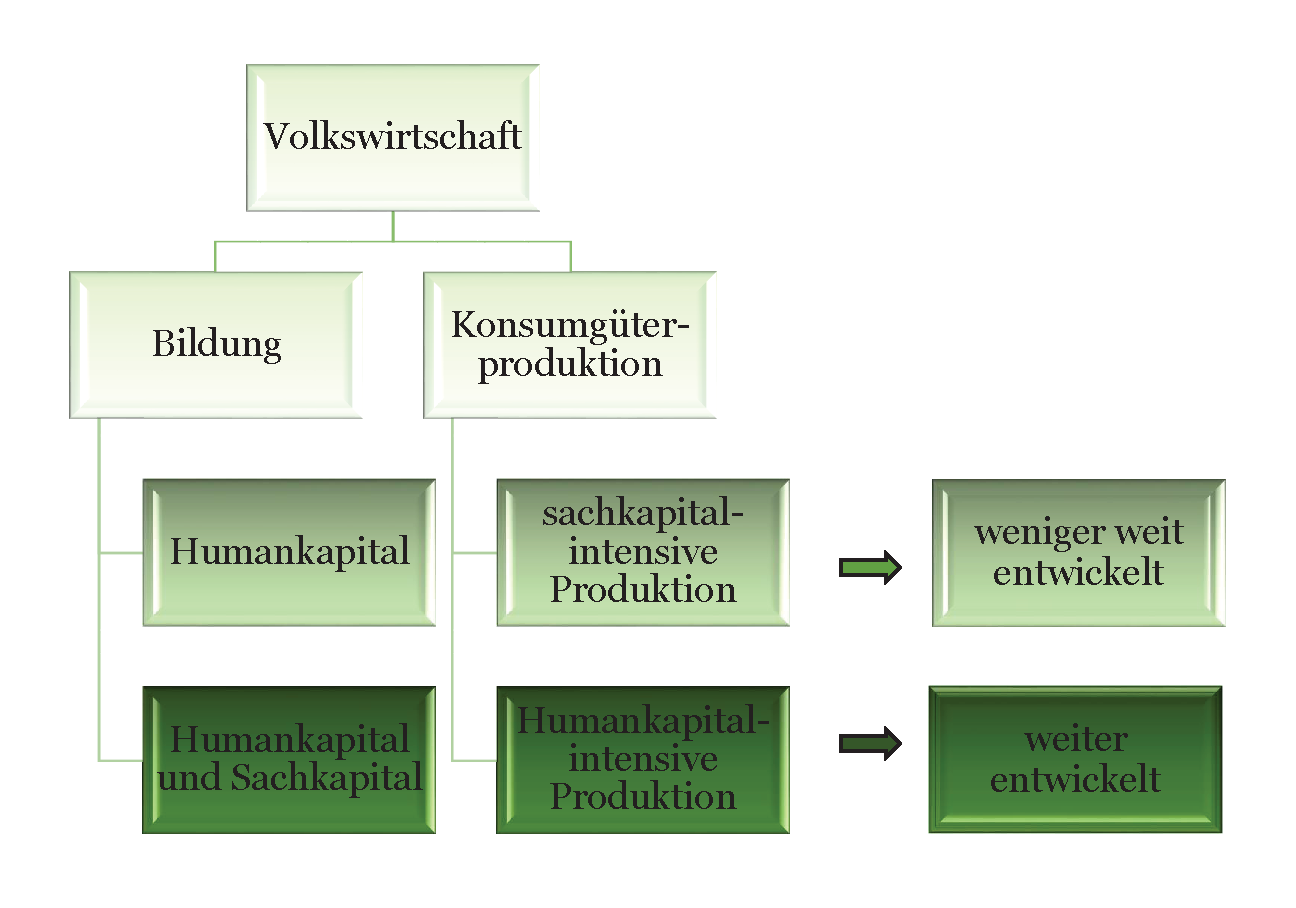
\includegraphics[width=0.7\textwidth]{C:/Users/BibiKiBa/Diss/Doktorarbeit/ModellEins/Abbildungen/SchemaPapierZwei.eps}
	\\
		\hfill\footnotesize\sffamily{\textbf{Quelle:}}  ENTWURF! eigene Darstellung
		\caption{Kategorisierung der Entwicklungsstufen}
		\label{fig:SchemaPapierZwei}		
\end{figure*}
In einer �konomisch kleinen Volkswirtschaft gibt es die beiden Sektoren G�terproduktion und Bildung. Im Konsumgutsektor wird ein Gut produziert, hier die Handtasche, die einem repr�sentativen Haushalt einen Nutzen stiftet. Der Nutzen besteht in diesem Fall aus der Bed�rfnisbefriedigung etwas von einem Ort zu einem anderen transportieren zu k�nnen. F�r die Herstellung des Gutes werden grunds�tzlich physisches Kapital sowie auch Humankapital ben�tigt. Beide Produktionsfaktoren k�nnen jedoch gegeneinander substituiert werden und das Gut kann je nach Einsatzverh�ltnissen relativ sachkapitalintensiv oder humankapitalintensiv produziert werden. Auf das Beispiel bezogen bedeutet dies, dass eine Handtasche von speziell ausgebildeten T�schnern in Handarbeit hergestellt wird. Der Herstellungsprozess ist sehr aufwendig, detailorientiert und erfordert besondere F�higkeiten und Fertigkeiten. Diese qualifizierte Arbeit ist sehr knapp und wird dementsprechend hochpreisig entlohnt. Ein konkretes Beispiel ist die in Frankreich gefertigte Birkin Bag der Marke Hermes, bei der weltweit nur wenige Menschen in der Lage sind diese mit den entsprechenden Qualit�tsanforderungen herzustellen.\\
Jedoch kann eine Handtasche den gleichen Zweck erf�llen, wenn ihr Produktionsprozess durch weniger qualifizierte Arbeit und deutlich st�rkeren Maschineneinsatz gepr�gt ist.
Ein Land wie beispielsweise Bangladesch, das spezialisiert ist auf die Textilindustrie, weist zwar eine relativ hohe Ausstattung an Arbeit vor, jedoch mit geringf�gigeren Qualifikationen als Frankreich. Ein Gro{\ss}teil der arbeitenden Bev�lkerung dieser Branche wird eine Industrien�hmaschine bedienen k�nnen und auch weitere handwerkliche F�higkeiten haben, jedoch sind die Arbeitsabl�ufe stark durch Arbeitsteilung gepr�gt und ein umsichtig allumfassender �berblick sowie eine fachkundige Einsch�tzung des Herstellungsprozesses fehlt. Der Schwerpunkt liegt dann auf der starken Spezialisierung jedes einzelnen Arbeiters auf einfache Arbeitsschritte, ohne dabei jedoch andere F�higkeiten zu f�rdern. Somit k�nnen auch die Folgen und Konsequenzen einer Neuerung schlecht eingesch�tzt werden. 
Neben der Unterscheidung des Produktionsprozesses im Konsumg�tersektor wird auch der Bildungssektor hinsichtlich der Einsatzfaktoren differenziert. So besteht grunds�tzlich die M�glichkeit nur durch den Einsatz von Lehrkr�ften, hier bereits ausgebildete Schneider, die F�higkeiten auf weniger qualifizierte Arbeiter auszuweiten. 
Ebenfalls denkbar ist neben dem Einsatz von Lehrkr�ften ein zus�tzlicher Einsatz von Sachkapital wie N�hmaschinen, B�cher oder Lehrvideos.\\
Auf Grundlage dieser Differenzierungsm�glichkeiten werden in diesem Kapitel verschiedene Entwicklungsstadien unterschieden. Demzufolge wird in einem relativ weniger weit entwickelten Land tendenziell mehr Sachkapital als Humankapital vorhanden sein und entsprechend die Produktionsstruktur diesem Umstand angepasst, also relativ sachkapitalintensiv produzieren. Hinzu kommt, dass meist auf den Einsatz von physischem Kapital im Bildungssektor verzichtet wird.\\
Bei einem relativ weiter entwickeltem Land wird angenommen, dass relativ gesehen mehr Humankapital als Sachkapital vorhanden ist, verglichen mit einem Land oder Region, das weniger weit entwickelt ist. Dies f�hrt zu einer humankapitalintensiven Produktion im Konsumgutsektor und zu einer Optimierung des Bildungssektors durch den Einsatz beider Produktionsfaktoren. 

\section{Autarkie}
Zun�chst wird die Situation ohne Handel betrachtet. Es wird ebenfalls ein zwei Sektor-Modell vorgestellt, dass sich noch stark an der Arbeit von \citet{Lucas.1988} orientiert. Bei dem einen Sektor handelt es sich um einen Konsum- bzw. Investitionsgutsektor bei dem anderen um den Bildungssektor.
\subsection*{Produktion}
In dem vorliegenden Modell einer geschlossenen Volkswirtschaft k�nnen die beiden Produktionsfaktoren physisches Kapital $K(t)$ und Arbeit $L(t)$ f�r den Konsumgut- oder Bildungssektor verwendet werden. 
Dabei wird angenommen, dass sich die Faktoren frei zwischen den beiden Sektoren bewegen k�nnen und demzufolge keine Anforderungen erf�llen m�ssen, um in den anderen Sektor zu wechseln. Die Mobilit�t der Faktoren f�hrt zu einem Ausgleich der Faktorpreise \citep{Samuelson.1941}. F�r physisches Kapital muss ein Zinssatz $r$ an die Kapitalgeber entrichtet werden und die Arbeiter erhalten den Lohnsatz $w$. Dabei ist der Preis f�r die Arbeit $w$ exogen gegeben und steigt nicht mit zus�tzlicher Bildung an. Der Faktor Arbeit h�ngt von der Bev�lkerungsgr�{\ss}e $N(t)$ eines Landes ab sowie vom durchschnittlichen Humankapitalbestand $h(t)$ und dem Anteil des Humankapitals $u(t)$, der in die Produktion des Konsumgutsektors eingeht.
\begin{equation}
L(t)=N(t)u(t)h(t)
\label{eq:Arbeit}
\end{equation}
Das physische Kapital setzt sich zusammen aus dem durchschnittlichen Kapitalbestand $k(t)$ und dem Anteil des physischen Kapitals $v(t)$, der ebenfalls bei der Produktion des Konsumgutes verwendet wird. 
\begin{equation}
K(t)=v(t)k(t)
\label{eq:Kapital}
\end{equation}
Die Produktionsfunktionen sind linear homogen und demnach liegen konstante Skalenertr�ge vor. Bei der Konsumg�terproduktion f�hrt der erh�hte Einsatz von Produktionsfaktoren zu einem proportionalen Anstieg der Ausbringungsmenge.
\begin{equation}
\text{Konsumgutsektor:}\qquad F[K,L]= A(v(t)k(t))^\alpha(u(t)h(t))^{1-\alpha}
\label{eq:ProduktionsfunktionK}
\end{equation}
Das Gut kann abh�ngig von der Produktionselastizit�t $\alpha$ mit relativ viel physischem Kapital oder Humankapital produziert werden. Demnach kann die Handtasche durch vollst�ndige Eigenleistung von qualifizierten T�schnern hergestellt werden, oder durch den verst�rkten Einsatz von Maschinen bspw. w�hrend des Zuschneideprozesses.\\
Im Bildungssektor bedeutet konstante Skalenertr�ge, dass jede zus�tzliche Einheit Bildung zu dem gleichen Lernerfolg f�hrt.\footnote{Diese Annahme weicht insofern von der Realit�t ab, als das Bildung einen abnehmenden Grenzertrag aufweisen kann. Der zus�tzliche Nutzen des "`Addierens"' und "`Subtrahierens"' ist h�her als eine "`Wurzel ziehen"' zu k�nnen. Deshalb wird auf gesamtwirtschaftlicher Ebene weiterhin von abnehmenden Grenzertr�gen ausgegangen, jedoch nicht auf der Ebene des Haushalts, der hier den Nutzen maximiert.} 
\begin{equation}
\text{Bildungssektor:} \qquad G[K,L]= B((1-v(t))k(t))^{\eta}((1-u(t))h(t))^{1-\eta}
\label{eq:ProduktionsfunktionH}
\end{equation}
Ebenso kann der Bildungssektor erweitert werden, durch den Einsatz von relativ viel physischem Kapital, wenn die Produktionselastizit�t $\eta$ hoch ist, oder eher humankapitalintensiv, wenn $\eta$ gering ist. Auch im Lernprozess spielt das Einsatzverh�ltnis eine Rolle. Angenommen es wird einer Gruppe von Schneiderlehrlingen durch die Lehrkraft an einem Beispiel mit nur einer N�hmaschine ein Prozess vorgef�hrt, ist der Lernerfolg ein anderer, als wenn jeder einzelne die M�glichkeit hat an einer eigenen N�hmaschine die neue Technik beliebig oft zu wiederholen und zu �ben.  \\
Die Aufteilung der Produktionsfaktoren auf die Sektoren wird dargestellt durch die Anteile $u(t)$ bzw. $v(t)$. Das physische Kapital wird im Konsumsektor verwendet mit $v(t)$ und im Bildungssektor mit $(1-v(t))$. Um das Beispiel der Textilindustrie aufzugreifen, w�re physisches Kapital bei der Produktion einer Handtasche die Nadel, bzw. die N�hmaschine. Dieses kann entweder dazu verwendet werden tats�chlich G�ter zu produzieren, oder aber um die Qualifikationen zu erweitern und den Lernprozess zu beschleunigen, indem man das neu gewonnene Wissen direkt anwendet. Ganz �hnlich erfolgt die Aufteilung des Humankapitals. Der Anteil $u(t)$ des Humankapitals wird f�r die Herstellung des Konsumgutes eingesetzt, wohingegen $(1-u(t))$  in den Bildungssektor eingeht. Auch hier kann das Wissen eines Einzelnen �ber die Zuschnitttechniken oder S�uberungsarbeiten  bei der Herstellung des Gutes eingesetzt werden, oder als Multiplikator im Bildungssektor, indem das vorhandene Wissen an bislang Unwissende weiter getragen wird.
\subsection*{Konsum}
Die Gesamtheit aller Haushalte richtet sich nach der Bev�lkerungsgr�{\ss}e eines Landes, die mit der exogenen Rate $n$ �ber die Zeit $t$ w�chst und von der anf�nglichen Bev�lkerungsgr�{\ss}e $N_0$ ausgeht.  
\begin{equation}
N(t)=N_0e^{nt}
\label{eq:Bevolkerungsentwickung}
\end{equation}
Die von den Unternehmen nachgefragten Produktionsfaktoren physisches Kapital und Humankapital bieten die Haushalte �ber die Faktorm�rkte an. Sie haben die Wahl die Konsumg�ter zu verbrauchen oder diese in zuk�nftigen Konsum zu investieren, also zu sparen und dadurch Kapital zu akkumulieren. 
Es wird angenommen, dass alle Haushalte die gleichen Pr�ferenzen haben und sie ihren Nutzen intertemporal maximieren. Auch hier wird von der Symmetrie der Haushalte ausgegangen und sie diskontieren ihren zuk�nftigen Nutzen mit der gleichen Rate, $\rho$. Der zuk�nftige Nutzen ist ihnen weniger wert, als der heutige Nutzen, demnach gilt, dass $\rho>0$. 
\begin{equation}
V=\int \limits_{0}^\infty  \! e^{-\rho t}\psi(c(t)) \, dt
\end{equation}
Der angef�hrte Lebenszeitnutzen $V$ bei einem unendlichen Zeithorizont ergibt sich aus der Gesamtheit aller jeweils gegenw�rtigen Nutzenwerte zu den verschiedenen Zeitpunkten. Die Zeitpunkte sind additiv separabel miteinander verkn�pft. Demnach wird der aus dem Konsum resultierende Nutzen in jedem Zeitpunkt neu bewertet und wird unabh�ngig von der Bewertung zu einem anderen Zeitpunkt sein.
\begin{equation}
\psi(c(t))=\frac{c(t)^{1-\sigma}}{1-\sigma}
\end{equation} 
Der gegenw�rtige Nutzen der Haushalte $\psi(t)$ ist nur von der konsumierten Menge der G�ter $c(t)$ abh�ngig, nicht vom Bildungsniveau. Au{\ss}erdem ist der Konsum zwischen den Zeitpunkten intertemporal variabel, in welchem Ausma{\ss} der Konsum zwischen zwei Zeitpunkten substituiert werden kann, h�ngt von der intertemporalen Substitutionselastizit�t $\sigma$ ab.\\
Die Maximierung des intertemporalen Nutzens l�sst die Haushalte einen optimalen Konsumpfad w�hlen. Dabei m�ssen sie sich entscheiden zwischen dem Konsum  des Gutes oder der Investition in den Kapitalstock. Hinzu kommen die Entscheidungen hinsichtlich der Aufteilung des physischen Kapitals und Humankapitals auf die beiden Sektoren, welche Aussagen �ber die Pr�ferenzen der Haushalte, bez�glich des Konsums und der Bildung zul�sst. Demzufolge sind die Entscheidungsvariablen des folgenden Maximierungsproblems die Konsummenge $c(t)$, der Anteil des physischen Kapitals, der in die Produktion des Konsumgutes eingeht $v(t)$ und dar�ber gleichzeitig den Humankapitalsektor determiniert, wegen $(1-v(t))$, sowie der Aufteilung des Humankapitals durch $u(t)$ auf die beiden Sektoren.\\
Die dynamische Betrachtung des zu maximierenden Lebenszeitnutzens $V$ verl�uft �ber den Zeithorizont von $0$ bis $\infty$ und beginnt mit den Anfangswerten des Kapitals $k_0$ und $h_0$.\footnote{Die beiden Startwerte $k_0$ und $h_0$ sind exogen.}
\begin{equation}\operatorname*{max}_{c(t),u(t),v(t)}V[k_0,h_0]= \int_{0}^\infty e^{-\rho t} \frac{c(t)^{1-\sigma}}{1-\sigma}dt\end{equation}
Der Nutzen wird nur dann maximal, wenn die beiden Ver�nderungen der Kapitalst�cke �ber die Zeit ber�cksichtigt werden. Denn durch jede zus�tzliche Einheit Kapital ver�ndert sich der Lebenszeitnutzen. Durch einen gegenw�rtigen Aufbau eines Kapitalstocks kann zuk�nftig mehr Nutzen generiert werden. Es besteht also eine direkte Abh�ngigkeit zwischen den Bewegungsgleichungen von Sach- und Humankapital, $\dot{k}$ und $\dot{h}$, sowie dem Lebenszeitnutzen.
		\begin{equation}\dot{k}(t)=A(v(t)k(t))^\alpha(u(t)h(t))^{1-\alpha}-c(t)\end{equation}\vspace{-0.8cm}
		\begin{equation} \dot{h}(t)=B((1-v(t))k(t))^{\eta}((1-u(t))h(t))^{1-\eta}\end{equation}
		\vspace{-0.3cm}
		\begin{displaymath} c(t)\geq 0,\quad k(t)\geq 0,\quad h(t)\geq 0, \end{displaymath}
		\begin{displaymath} 0\leq u(t)\leq 1,\quad 0\leq v(t) \leq1, \end{displaymath}
		\begin{displaymath} 0\leq \alpha\leq 1,\quad 0\leq \eta \leq1, \quad A\geq 0, \quad B\geq 0\end{displaymath}
Das Sachkapital erh�ht sich durch all die produzierten G�ter, die nicht konsumiert werden. Der Produktion der G�ter dient sowohl physisches Kapital als auch Humankapital. Bei $A$ handelt es sich um einen Technologieparameter, der das technische Wissen im Konsumgutsektor ber�cksichtigt. Humankapital wird ebenfalls durch beide Kapitalarten aufgebaut und durch den Technologieparameter $B$ beeinflusst. Dabei gehen die Produktionsfaktoren jeweils mit einer Produktionselastizit�t von $\alpha$ bzw. $\eta$ in den jeweiligen Prozess ein.\\
Da es sich um ein intertemporales Optimierungsproblem handelt, ist es mit der Hamilton Funktion zu l�sen. Dieses Verfahren wird auch Maximumprinzip genannt und geht zur�ck auf \citep{Pontryagin.1964}. Es beschreibt den optimalen Konsumpfad, der den Lebenszeitnutzen, unter Ber�cksichtigung der Entscheidungen der Haushalte �ber $c(t)$, $u(t)$ und $v(t)$ maximiert. Diese Entscheidungsvariablen determinieren die zuk�nftige Ausweitung der Kapitalst�cke $k(t)$ und $h(t)$. Es besteht zu jedem Zeitpunkt eine Abh�ngigkeit des Lebenszeitnutzens zu dem jeweils gegenw�rtig vorhandenem physischen Kapitalstock und Humankapitalstock, sowie zu den Entscheidungen des Haushalts �ber die Aufteilung der Ressourcen auf die beiden Sektoren.\footnote{Ressourccen eines Haushalts k�nnen die Zeit, Kraft oder auch die Konzentration sein.} Deshalb sind f�r die L�sung des dynamischen Maximierungsproblems die Bewegungsgleichungen von $h(t)$ und $k(t)$ notwendig, da diese die jeweilige Ver�nderung der Kapitalst�cke �ber die Zeit beschreiben.\footnote{Aus Gr�nden der Anschaulichkeit wird im folgenden die Abh�ngigkeit der Variablen gegen�ber der Zeit $t$ vernachl�ssigt.}
\begin{equation}
\begin{split}
\mathbb{H}=&~e^{-\rho t}\frac{c^{1-\sigma}}{1-\sigma}\\
&+\gamma_1(A(vk)^\alpha(uh)^{1-\alpha}-c)\\
&+\gamma_2B[(1-v)k]^{\eta}[(1-u)h]^{1-\eta}\\
\end{split}
\end{equation}
\begin{displaymath} \gamma_1 > 0,\quad \gamma_2 > 0 \end{displaymath}
Die Optimierung �ber die Hamiltonfunktion gibt Auskunft �ber den resultierenden Gesamtnutzen f�r die anberaumte Lebenszeit. Au{\ss}erdem ist ein Vergleich resultierender Nutzwerte zweier aufeinanderfolgender Zeitpunkte m�glich. Der erste Summand beschreibt den gegenw�rtigen Nutzeneffekt herbeigef�hrt durch den Konsum von G�tern, der wiederum �ber die Entscheidungsvariablen determineirt wird. Die folgenden Summanden der Hamiltonian stellen die zuk�nftigen Nutzeneffekte der zuk�nftigen Ver�nderungen des Sach- und Humankapitals dar, dessen gegenw�rtige Nutzwerte durch die zugeh{\"o}rigen Schattenpreise $\gamma_1$ und $\gamma_2$ ausgedr�ckt werden.\footnote{Bei den Variablen $\gamma_1$ und $\gamma_2$ handelt es sich origin�r um Hilfsvariablen oder auch als Schlupfvariablen bekannt, die hier als Schattenpreis interpretiert werden k�nnen.} Die Schattenpreise ergeben sich aus der Ableitung des Lebenszeitnutzens nach jeweils einem Produktionsfaktor und sind somit der Lebenszeitgrenznutzen einer Einheit Sach- oder Humankapital. Dieser dr�ckt den Wert einer zus�tzlichen Einheit Kapital f�r den gesamten Zeithorizont aus, also eine m�gliche marginale Lebenszeitnutzenverbesserung durch eine zus�tzliche Einheit Kapital.  Beide Schattenpreise sind positiv, da ansonsten eine Einsatzfaktor�nderung zu einer Indifferenz der Haushalte f�hrt. Denn bei einem Schattenpreis von Null w�rde der zuk�nftige Nutzen den Lebenszeitnutzen nicht tangieren und der Fokus auf der Gegenwart liegen ohne zuk�nftige Zeitpunkte zu ber�cksichtigen. Durch die Multiplikation mit dem Schattenpreis wird der Nutzwert der Kapitalerh�hung ber�cksichtigt. Der Schattenpreis "`konvertiert"' die Faktoreinheiten in Nutzeinheiten unter Ber�cksichtigung der zeitlichen Ver�nderung. Beide Nutzeneffekte konkurrieren miteinander, da ein gegenw�rtiger Konsum den zuk�nftigen mindert \citep{Chiang.2000,Chiang.2011}.\\   
Diese Optimierung findet f�r alle m�glichen Zeitpunkte statt und erm�glicht eine Vergleichbarkeit zweier aufeinanderfolgender Zeitpunkte. Erst dann wenn der heutige Grenznutzen mit dem morgigen �bereinstimmt, wurde der optimale Konsumpfad einer Volkswirtschaft gefunden \citep{Chiang.2000}. Folgende Bedingungen erster Ordnung l�sen das Optimierungsproblem.\footnote{Die ausf�hrliche Berechnung aller Gleichgewichtsbedingungen sind in Appendix \ref{AutarkieAPPENDIX} zu finden.}  
\begin{align}
&\frac{\partial\mathbb{H}}{\partial c}\overset{!}{=}~0\label{eq:foc1WM}\\
&\frac{\partial\mathbb{H}}{\partial v}\overset{!}{=}~0\label{eq:foc2WM}\\
&\frac{\partial\mathbb{H}}{\partial k}\overset{!}{=}-\dot{\gamma_1}\label{eq:foc3WM}\\
&\frac{\partial\mathbb{H}}{\partial u}\overset{!}{=}~0\label{eq:foc4WM}\\
&\frac{\partial\mathbb{H}}{\partial h}\overset{!}{=}-\dot{\gamma_2}\label{eq:foc5WM}\end{align}
Die Bedingungen erster Ordnung werden im Folgenden recht allgemein, jedoch sehr ausf�hrlich beschrieben, um in der folgenden Analyse hinsichtlich verschiedener Entwicklungsst�nde gr�{\ss}tenteils darauf verzichten zu k�nnen. 
\subsubsection*{Ableitung nach Zustandsvariablen, $k$ und $h$}
Die Ableitung nach einer Zustandsvariablen wird mit der jeweiligen negativen Bewegungsgleichung des Schattenpreises gleichgesetzt.\footnote{Der Lebenszeitgrenznutzen einer zus�tzlichen Einheit $\gamma$ ist zwar positiv, jedoch abnehmend mit zunehmendem Kapitaleinsatz �ber die Zeit. Demzufolge ist die Ableitung des Schattenpreises nach der Zeit negativ. Das negative Vorzeichen gleicht diesen Zusammenhang aus und es kann eine Gleichheit beider Seiten herbeigef�hrt werden.} Dabei handelt es sich um eine intertemporale Arbitragebedingung, die gleich dem jeweiligen negativen Lebenszeitgrenznutzen sein soll. Die Abnahme des Schattenpreises �ber die Zeit $\dot{\gamma}$ kann auch als Abschreibungsrate des Schattenpreises interpretiert werden und soll genau so gro{\ss} sein, wie die Erh�hung des gegenw�rtigen und zuk�nftigen Nutzen durch die Kapitalakkumulation. Erst wenn sich beide Gr�{\ss}en ausgeglichen haben, kann der Lebenszeitnutzen maximal sein \citep{Chiang.2000,Chiang.2011}.

\subsubsection*{Ableitung nach Entscheidungsvariablen $v$,$u$ und $c$ }
Die Ableitung nach einer Zustandsvariablen ergibt die optimale Allokation eines Produktionsfaktors in jedem Sektor zu jedem Zeitpunkt. Die Gleichsetzung der Ableitung einer Entscheidungsvariablen mit $0$ bedeutet, dass dann diese Variable maximal sein wird, unter der Voraussetzung, dass die Bedingung der jeweils zugeh�rigen Zustandsvariablen erf{\"u}llt ist.\newline 
Die Entscheidungsvariable wird direkt vom Wirtschaftssubjekt gew�hlt, aus ihr ergibt sich dann indirekt die Zustandsvariable \citep{Chiang.2011}. Die Haushalte entscheiden sich sowohl f�r den Konsum, als auch f�r die Aufteilung der eigenen Ressourcen, die ihren Nutzen maximieren. Dabei muss, um beim anf�nglichen Beispiel zu bleiben, ber�cksichtigt werden, wie viele Handtaschen sie derzeit konsumieren m�chten und wie viel Sachkapital, wie Nadeln, N�hmaschinen oder Scheren  sie bereit sind f�r die Produktion bzw. f�r ihre Weiterbildung zu den unterschiedlichen Zeitpunkten zu investieren. 

\subsubsection*{Ableitung nach $c$}
Durch die Ableitung der Hamiltonian nach dem Konsum $c$, siehe \colorbox{lightgray}{Gleichung \eqref{eq:foc1WM}}, wird der maximale Konsum unter Ber{\"u}cksichtigung der Nebenbedingungen $\dot{k}$ und $\dot{h}$ bestimmt.
\begin{equation}
\colorbox{lightgray}{$\partial\mathbb{H}/\partial c\overset{!}{=}~0$}
\end{equation}
\vspace{-0.5cm}
\begin{equation}
e^{-\rho t}c^{-\sigma}-\gamma_1 = 0
\end{equation}
\vspace{-0.7cm}
\begin{equation}
\gamma_1=e^{-\rho t}c^{-\sigma}
\label{eq:foc1WMa}
\end{equation}
Die Gleichung \eqref{eq:foc1WMa} dr{\"u}ckt aus, dass der diskontierte Grenznutzen des optimalen Konsums pro Kopf gleich dem gegenw�rtigen Schattenpreis $\gamma_1$ einer zus�tzlichen Sachkapitaleinheit ist. Da auch die zweite Ableitung nach $c$ kleiner $0$ ist, handelt es sich um einen maximalen Punkt. 
\begin{equation}
-e^{-\rho t}\sigma c^{-\sigma-1}<0
\end{equation}
Der Schattenpreis beschreibt in diesem Fall wie hoch die Lebenszeitnutzenerh�hung ist, wenn auf den heutigen Konsum verzichtet wird und welchen zuk�nftigen Nutzenwert die  daraus resultierende Kapitalakkumulation stiften wird.\\
Die optimale Konsumg�termenge beeinflusst im Wesentlichen die Sachkapitalakkumulation. Die Entscheidung des Haushalts �ber die gegenw�rtige Konsummenge an Handtaschen bedingt die Akkumulation von Handtaschen und den damit verbundenen G�terberg. Denn je mehr konsumiert wird, desto weniger G�tereinheiten k�nnen in die Kapitalakkumulation investiert werden. Demzufolge ist f�r die weitere Analyse eine Ableitung der Zustandsvariablen $k$ notwendig.
 
\subsubsection*{Ableitung nach $k$}
Bei der Variablen $k$ handelt es sich um eine Zustandsvariable, die den aus der Konsumentscheidung resultierenden Zustand angibt. Neben dem Konsum beeinflusst auch die Aufteilung des Sachkapitals auf die beiden Sektoren $v$ den Kapitalbestand. Steigt der Kapitalstock um eine Einheit an, dann erh�ht sich der Lebenszeitnutzen um den Schattenpreis, der den Wert dieser zus�tzlichen Kapitaleinheit in Nutzeneinheiten angibt. Diese Auswirkung auf den Nutzen durch die Ver�nderung einer Einheit Sachkapital beschreibt \colorbox{lightgray}{Gleichung \eqref{eq:foc3WM}}. Der gegenw�rtige Grenznutzen des physischen Kapitals soll also dem zuk�nftigen Nutzen einer Einheit Sachkapital entsprechen. Der Einsatz einer zus�tzlichen N�hmaschine f�hrt im Konsumg�tersektor zu einer erh�hten Produktion von Handtaschen, die entweder f�r den Eigenbedarf genutzt werden k�nnen oder aber den Kapitalstock erh�hen. Es besteht jedoch auch die M�glichkeit die Sachkapitaleinheit in den Bildungssektor f�r das Erlernen neuer effizienterer N�htechniken zu investieren. In beiden F�llen erh�ht sich der Lebenszeitnutzen, entweder durch den gegenw�rtigen oder durch den zuk�nftigen Konsum. Die H�he des zus�tzlichen k�nftigen Nutzens wird am Schattenpreis bemessen. So gilt f{\"u}r die erste Ableitung der Hamiltonian nach dem physischen Kapital $k$, dass diese im Gleichgewicht der negativen ersten Ableitung nach der Zeit des Schattenpreises von Sachkapital entspricht. 
\begin{equation}
\colorbox{lightgray}{$\partial\mathbb{H}/\partial k\overset{!}{=}-\dot{\gamma_1}$}\label{nachK}
\end{equation}
\begin{equation}
\gamma_{1}A v^{\alpha}k^{\alpha -1} \alpha(u h)^{1- \alpha} + \gamma_{2}B(1- v)^{\eta} k^{\eta -1} \eta \left [ (1-u)h \right ]^{1- \eta}\overset{!}{=} - \dot{\gamma}_{1}\label{BedingungFoc3WM}
\end{equation}

Der gegenw�rtige Nutzwert der auf Human- und Sachkapitalakkumulation zur�ckzuf�hren ist, soll dem zuk�nftigen Nutzwert entsprechen. Der Schattenpreis $\gamma_1$ wird mit der Rate abgeschrieben, mit der die k�nftige Kapitalakkumulation zur Lebenszeitnutzenerh�hung beitr�gt. Erst wenn diese Bedingung erf�llt ist kann der Nutzen maximal sein \citep{Chiang.2000}.

\subsubsection*{Ableitung nach $v$}
Bei der Aufteilung des Sachkapitals den Konsumgutsektor und den Bildungssektor $v$, handelt es sich ebenfalls um eine Entscheidungsvariable. Indem eine marginale Ver�nderung dieser Aufteilung auf den Nutzen gleich null gesetzt wird, kann der Nutzen maximiert werden, sofern die Bedingung gem�{\ss} Gleichung \eqref{BedingungFoc3WM} erf�llt ist.
Wird die allgemeine Form aus \colorbox{lightgray}{Gleichung \eqref{eq:foc2WM}} hier konkret ausformuliert ergibt sich:
\begin{equation}
\colorbox{lightgray}{$\partial\mathbb{H}/\partial v\overset{!}{=}~0$}
\end{equation}
\vspace{-0.5cm}
\begin{equation}
\gamma_1A\alpha v^{\alpha-1}k^\alpha(uh)^{1-\alpha}-\gamma_2B\eta(1-v)^{\eta-1}k^\eta[(1-u)h]^{1-\eta}\overset{!}{=}~0
\end{equation}
\vspace{-0.7cm}
\begin{equation}
\gamma_1A\alpha v^{\alpha-1}k^\alpha(uh)^{1-\alpha}=\gamma_2B\eta(1-v)^{\eta-1}k^\eta[(1-u)h]^{1-\eta}
\end{equation}
Demzufolge sollen sich die mit dem Schattenpreis bewerteten Grenzprodukte entsprechen. Eine zuk�nftige marginale Ver�nderung von $u$ bedingt im Konsumgutsektor einen anteilig h�heren Einsatz von Sachkapital um den der Anteil im Bildungssektor dadurch reduziert wird. Der resultierende zus�tzliche Nutzen des Kapitaleinsatzes im Konsumgutsektor soll die Minderung des Nutzens im Bildungssektor ausgleichen. Durch den Einsatz einer N�hmaschine in der Textilindustrie kommt es zu einer Nutzensteigerung, die genau der Nutzenminderung im Bildungssektor entsprechen muss. 

\subsubsection*{Ableitung nach $h$}
Auch im Bildungssektor soll sich die Ver�nderung der Lebenszeitgrenznutzen zweier aufeinanderfolgender Perioden entsprechen. Diesen Zusammenhang beschreibt \colorbox{lightgray}{Gleichung \eqref{eq:foc5WM}}. Der Grenznutzen des Humankapitals beschreibt eine Ver�nderung der Hamiltonian durch einen Anstieg um eine Einheit Humankapital und soll heute genau soviel Nutzen stiften wie in der folgenden Periode.
\begin{equation}
\colorbox{lightgray}{$\partial\mathbb{H}/\partial h\overset{!}{=}-\dot{\gamma_2}$}\label{nachH}
\end{equation}
\begin{equation}
\gamma_1A(1-\alpha)(vk)^\alpha u^{1-\alpha}h^{-\alpha}+\gamma_2 B(1-\eta)[(1-v)k]^{\eta}(1-u)^{1-\eta}h^{-\eta}\overset{!}{=}-\dot{\gamma}_2\label{GNHK}
\end{equation}
Dies ist genau dann erf�llt, wenn der zuk�nftige Nutzenwert der zus�tzlichen Humankapitaleinheit dem heutigen Grenznutzen entspricht, da der Schattenpreis mit einer Rate von $-\gamma_2$ abgeschrieben wird. Der gegenw�rtige Nutzengewinn aus einer Einheit qualifizierter Arbeit entspricht dem zuk�nftigen Nutzen durch den Einsatz selbiger in den Bildungssektor. Es sollte demnach im Gleichgewicht keinen Unterschied machen, wann ein ausgebildeter Schneider eingesetzt wird. 

\subsubsection*{Ableitung nach $u$}
Ist die Bedingung \eqref{GNHK} erf�llt, dann kann $u$ so gew�hlt werden, dass die Hamiltonian zu jedem Zeitpunkt maximal ist, indem \colorbox{lightgray}{Gleichung \eqref{eq:foc4WM}} gilt.
\begin{equation}
\colorbox{lightgray}{$\partial\mathbb{H}/\partial u\overset{!}{=}~0$}
\end{equation}
\vspace{-0.5cm}
\begin{equation}
\gamma_1A(1-\alpha)(vk)^{\alpha}h^{1-\alpha}u^{-\alpha}-\gamma_2B(1-\eta)[(1-v)k]^\eta (1-u)^{-\eta} h^{1-\eta}\overset{!}{=}0
\end{equation}
\vspace{-0.7cm}
\begin{equation}
\gamma_1A(1-\alpha)(vk)^{\alpha}h^{1-\alpha}u^{-\alpha}=\gamma_2B(1-\eta)[(1-v)k]^\eta (1-u)^{-\eta} h^{1-\eta}\label{foc4}
\end{equation}
Die Aufteilung f�hrt zu einem maximalen Nutzen, wenn sich die zuk�nftigen Grenzprodukte beider Sektoren entsprechen. Eine Umverteilung des Humankapitals muss in beiden Sektoren die gleiche Nutzenver�nderung herbeirufen. Dann ver�ndert sich der Lebenszeitnutzen nicht mehr durch eine Umverteilung des Einsatzortes des ausgebildeten T�schners.

\subsubsection*{Transversalit�tsbedingung}
Die Transversalit�tsbedingungen sind begrenzende Bedingungen der Schattenpreise. Sie gew�hrleisten, dass zum angenommen Endzeitpunkt des geplanten Zeithorizonts der Bestand der Zustandsvariablen vollst�ndig aufgebraucht oder deren Wert in H�he der Schattenpreise zum Planungsendzeitpunkt gleich $0$ ist \citep{Chiang.2000}.
%Sie beschreiben den Zeithorizont der zu treffenden Entscheidungen, hier �ber den Konsum, die Aufteilung des physisches Kapital und Humankapitals auf die beiden Sektoren.
\begin{equation} \lim_{t \to \infty}e^{-\rho t}\gamma_1k=0\end{equation}
\vspace{-0.7cm}
\begin{equation} \lim_{t \to \infty}e^{-\rho t}\gamma_2h=0\end{equation}

\subsection*{Gleichgewichtsbedingungen}
Fasst man die zuvor separat erl�uterten Bedingungen zusammen, dann ergibt sich ein Gleichungssystem, welches die notwendigen Bedingungen beschreibt, damit eine autarke Volkswirtschaft langfristig im Gleichgewicht ist. 
\begin{align}
&\gamma_1=e^{-\rho t}c^{-\sigma}\\
&\gamma_1A\alpha v^{\alpha-1}k^\alpha(uh)^{1-\alpha}=\gamma_2B\eta(1-v)^{\eta-1}k^\eta[(1-u)h]^{1-\eta}\\
&\gamma_{1}A v^{\alpha}k^{\alpha -1} \alpha(u h)^{1- \alpha} + \gamma_{2}B(1- v)^{\eta} k^{\eta -1} \eta \left [ (1-u)h \right ]^{1- \eta}= - \dot{\gamma}_{1}\label{foc3IL}\\
&\gamma_1A(1-\alpha)(vk)^{\alpha}h^{1-\alpha}u^{-\alpha}=\gamma_2B(1-\eta)[(1-v)k]^\eta (1-u)^{-\eta} h^{1-\eta}\\
&\gamma_1A(1-\alpha)(vk)^\alpha u^{1-\alpha}h^{-\alpha}+\gamma_2 B(1-\eta)[(1-v)k]^{\eta}(1-u)^{1-\eta}h^{-\eta}=-\dot{\gamma}_2
\end{align}
\vspace{-0.7cm}
\begin{equation} \lim_{t \to \infty}e^{-\rho t}\gamma_1k=0\end{equation}
\vspace{-0.7cm}
\begin{equation} \lim_{t \to \infty}e^{-\rho t}\gamma_2h=0\end{equation}
Aus diesen Bedingungen l�sst sich, wie in Appendix \ref{AutarkieAPPENDIX} dargestellt, das gleichgewichtige Wachstum herleiten. 

\subsubsection*{Keynes-Ramsey-Regel}
Die Keynes-Ramsey-Regel beschreibt in ihrer urspr�nglichen Form die Beziehung zwischen dem Grenzprodukt des Kapitals und dem daraus resultierenden Wirtschaftswachstum.  
\begin{equation}
\boxed{\hat{c}=\frac{1}{\sigma}\left(A\alpha \left(\frac{vk}{uh}\right)^{\alpha -1}-\rho\right)}\label{KRRWM}
\end{equation}
Je produktiver eine Einheit Sachkapital ist, desto h�her ist die Wachstumsrate. Es besteht ein positiver Zusammenhang zwischen dem Grenzprodukt des physischen Kapitals $A\alpha \left(\frac{vk}{uh}\right)^{\alpha -1}$ und der Wachstumsrate. Wohingegen ein negativer bzw. inverser Zusammenhang zwischen selbiger Wachstumsrate und dem Diskontfaktor $\rho$ besteht.\footnote{Der Kehrwert der intertemporalen Substitutionselastizit�t $1/\sigma$ ist ebenfalls positiv mit der Wachstumsrate verkn�pft. Je leichter man zwischen den Zeitpunkten substituieren kann, desto h�her ist die Wachstumsrate.} 
Diese Gleichung l�sst jedoch noch keine konkreten Aussagen �ber die tats�chliche Gr�{\ss}e der Variablen zu. So ist noch immer unklar wie hoch $u$ oder auch $v$ gew�hlt werden muss, um zum gleichgewichtigen Wachstumspfad zu konvergieren. Ebenso verh�lt es sich mit den Zustandsvariablen $k$ und $h$, auch hier ist noch unbekannt wie gro{\ss} diese im Gleichgewicht sind. Die Gleichgewichtswerte werden im folgenden Abschnitt \nameref{sec:Modelldynamik} beschrieben, deren Berechnung ist ausf�hrlich in Appendix \ref{AutarkieAPPENDIX} zu finden. 

\subsection*{Modelldynamik}\label{sec:Modelldynamik}
Gleichung \eqref{KRRWM} zeigt, wenn das Verh�ltnis $k/h$ und die Kapitalaufteilungen $u$ und $v$ konstant sind, dass dann der Konsum mit konstanter Rate w�chst. 
Betrachtet man das Wachstum des physischen Kapitals, dann sind ebenfalls das Verh�ltnis beider Kapitalarten $k/h$ sowie die Aufteilungen $v$ und $u$ relevant. Hinzu kommt das Verh�ltnis des Konsums zum physischen Kapital $c/k$ bzw. $\chi$.\footnote{Ersetzt man $\chi=\frac{c}{k}$ ergeben sich zwei Schreibweisen f�r die Wachstumsrate des physischen Kapitals.} Erst wenn diese konstant sind, w�chst das Sachkapital $k$ mit konstanter Rate.
\begin{equation}
\hat{k}=Av^\alpha k^{\alpha-1}(uh)^{1-\alpha}-\frac{c}{k} \qquad \hat{=} \qquad
\hat{k}=Av^\alpha k^{\alpha-1}(uh)^{1-\alpha}-\chi 
\end{equation}
Ganz �hnlich verh�lt es sich mit dem Humankapital. Hier m�ssen wieder $k/h$, $v$ und $u$ konstant sein, damit das Humankapitalwachstum konstant ist. 
\begin{equation}
\hat{h}=B\left[(1-v)\frac{k}{h}\right]^{\eta}(1-u)^{1-\eta}
\end{equation}
Verk�rzt durch $x_1=\frac{vk}{uh}$ und $x_2=\frac{(1-v)k}{(1-u)h}$ lassen sich diese Gleichungen auch schreiben als:
\begin{equation}
\boxed{\hat{k}=Ax_1^\alpha \frac{uh}{k}-\chi}
\end{equation}
\begin{equation}
\boxed{\hat{h}=Bx_2^\eta(1-u)}
\end{equation}
Es liegt nahe, dass im Steady-State gilt, dass $\hat{c}=\hat{k}=\hat{h}$ und somit die Wachstumsraten gleich gro{\ss} sind, wenn $k/h$, $c/k$, $u$ und $v$ konstante Gr�{\ss}en sind. 

Eine Volkswirtschaft befindet sich dann im Gleichgewicht, wenn sich die Verh�ltnisse der Grenzproduktivit�ten beider Sektoren entsprechen, die sich aus den Gleichungen \eqref{eq:foc2WM} und \eqref{eq:foc3WM} herleiten lassen. Eine Umverteilung des Kapitals zwischen den Sektoren stellt im Gleichgewicht keinen Sektor besser als zuvor. 
\begin{equation}
\boxed{\frac{1-\alpha}{\alpha}x_1=\frac{1-\eta}{\eta}x_2}
\end{equation}
Eine zus�tzliche Sach- oder Humankapitaleinheit weist im Konsumgutsektor die gleiche Grenzproduktivit�t auf wie im Bildungssektor. Dies ist dann der Fall, wenn sich die Schattenpreisverh�ltnisse in beiden Sektoren entsprechen und somit das Verh�ltnis der Lebenszeitgrenznutzen in beiden gleich gro{\ss} ist. Langfristig verhalten sich die Relationen $x_1$ und $x_2$ gleich und mit Hilfe der folgenden Gleichung \eqref{A5} k�nnen die Wachstumsraten $\hat{x}_1$ und $\hat{x}_2$ berechnet werden, die demnach im Gleichgewicht konstant sind. 
\begin{equation}
\hat{x}_1=\hat{x}_2=0
\end{equation}
Zur L�sung des Gleichungssystems ist eine weitere Bedingung notwendig, die sich aus Gleichung \eqref{nachK} und \eqref{nachH} herleiten l�sst. Diese dr�cken aus, dass zum einen die Rate des Lebenszeitgrenznutzens von Humankapital dem Grenzprodukt des Humankapitals entspricht. Zum anderen die Wachstumsrate des Schattenpreises des physischen Kapitals ebenso gleich dem Grenzprodukt des Kapitals im Konsumgutsektor ist. 
\begin{equation}
\boxed{B(1-\eta)x_2^\eta=-\rho-\sigma\hat{c}-\alpha\hat{x}_1+\eta\hat{x}_2}\label{A5}
\end{equation}
Der Nutzen aus einer zus�tzlichen Humankapitaleinheit im Bildungssektor ist gleich dem resultierenden Nutzen einer zus�tzlichen Einheit Sachkapital, da $\rho-\sigma\hat{c}=\hat{\gamma_1}=-A\alpha x_1^{\alpha-1}$ gem�{\ss} Gleichung \eqref{foc3IL}.
Demzufolge ergibt sich folgendes Gleichungssystem, welches das Gleichgewicht beschreibt. 
\begin{align}
&\hat{k}=Ax_1^\alpha \frac{uh}{k}-\chi\label{GG1WM}\\
&\hat{h}=Bx_2^\eta(1-u)\label{GG2WM}\\
& x_1(1-\alpha)/\alpha =x_2(1-\eta)/\eta\label{GG3WM}\\
&\hat{c}=\frac{1}{\sigma}\left(A\alpha x_1^{\alpha -1}-\rho\right)\label{GG4WM}\\
&B(1-\eta)x_2^\eta=-\rho-\sigma\hat{c}-\alpha\hat{x}_1+\eta\hat{x}_2\label{GG5WM}
\end{align}
Mithilfe dieses Gleichungssystems k�nnen die gleichgewichtigen Werte der verschiedenen Variablen bestimmt werden. Durch die Aufl�sung nach den optimalen Werten f�r $x_1$ und $x_2$ wird die Konsumwachstumsrate umgeformt in:\footnote{Siehe Appendix \ref{AutarkieAPPENDIX}.} 
\begin{equation}
\boxed{\hat{c}^*=\frac{1}{\sigma}\left(\left[A^\eta\alpha^{\alpha\eta}(1-\eta)^{(1-\eta)(1-\alpha)}(\eta(1-\alpha))^{\eta(1-\alpha)}B^{1-\alpha}\right]^\frac{1}{1+\eta-\alpha}-\rho\right)}
\end{equation}
Dabei h�ngt das Grenzprodukt $\left[A^\eta\alpha^{\alpha\eta}(1-\eta)^{(1-\eta)(1-\alpha)}(\eta(1-\alpha))^{\eta(1-\alpha)}B^{1-\alpha}\right]^\frac{1}{1+\eta-\alpha}$ von den Technologieparametern $A$ und $B$ beider Sektoren ab und wird im folgenden mit $M$ abgek�rzt. Durch jeglichen technologischen Fortschritt erh�ht sich das Wirtschaftswachstum.\\
Die gleichgewichtige Aufteilung des Humankapitals $u^*$ ist dadurch bedingt, dass im Gleichgewicht \colorbox{lightgray}{$\hat{c}=\hat{h}$} gilt.
\begin{equation}
\boxed{u^*=\frac{\sigma M-(1-\eta)(M-\rho)}{\sigma M}}\label{uOptAut}
\end{equation}
Im wesentlichen existiert eine Abh�ngigkeit der Humankapitalaufteilung $u$ zum Grenzprodukt des Kapitals $M$. Zwischen beiden besteht eine inverse Beziehung, somit wird ein abnehmendes Grenzprodukt des Kapitals durch den erh�hten Einsatz von Humankapital in den Konsumgutsektor kompensiert. Wenn jede zus�tzliche N�hmaschine im Konsumgutsektor nun weniger produktiv ist, als die zuvor Eingesetzte, wird die qualifizierte Arbeit nicht mehr im Konsumgutsektor zur Produktion eingesetzt, sondern stattdessen in den Bildungssekor investiert.  Je h�her die Zeitpr�ferenz $\rho$ ist, desto weniger wird Humankapital in den Bildungssektor investiert. Zuk�nftige m�glicherweise h�here Konsumm�glichkeiten durch den Einsatz qualifizierterer Arbeit haben eine geringere Bedeutung, als der heutige Konsum. Demzufolge besteht ein positiver Zusammenhang zwischen der Diskontrate und dem Anteil des Humankapitals, der in die Konsumg�terproduktion eingeht. Diese Gr�{\ss}e $u^*$ dient als Referenzwert und wird im folgenden die Wirkung der Offenheit verdeutlichen. 
F�r das physische Kapital ergibt sich die folgende optimale Aufteilung im Gleichgewicht. 
\begin{equation}
\boxed{
v^*=\frac{\alpha  (1-\eta ) \left(\frac{M}{B (1-\eta )}\right)^{1/\eta } (M \sigma -(1-\eta ) (M-\rho ))}{(1-\alpha ) \eta  M \sigma  \left(\frac{\alpha  (1-\eta ) \left(\frac{M}{B  (1-\eta )}\right)^{1/\eta } (M \sigma -(1-\eta ) (M-\rho ))}{(1-\alpha ) \eta  M \sigma }+\left(\frac{M}{B  (1-\eta )}\right)^{1/\eta } \left(1-\frac{M \sigma -(1-\eta ) (M-\rho )}{M \sigma }\right)\right)}}
\end{equation}
Ebenso wie bei $u^*$ aus \eqref{uOptAut} besteht zwischen der Aufteilung des Sachkapitals $v$ und dem Grenzprodukt des Kapitals $M$ ein inverser Zusammenhang,
 sowie ein positiver zu der Diskontrate $\rho$. Je h�her das Grenzprodukt ist, desto weniger physisches Kapital ist notwendig um das gleiche Outputniveau zu erzielen. Es m�ssen weniger N�hmaschinen eingesetzt werden, da nun jede Maschine produktiver ist. Das �bersch�ssige Sachkapital wird nun in den Bildungssektor flie{\ss}en und dort die Produktivit�t steigern. 
Die Relation des Konsums zum physischen Kapital $\chi$ kann durch \colorbox{lightgray}{$\hat{c}=\hat{k}$} ermittelt werden.
\begin{equation}
\boxed{\chi^*=\frac{1}{\sigma}\left(\frac{A\alpha \sigma[-\eta\rho+M(\eta+\sigma-1)+\rho] \left(\frac{\alpha  (\eta -1) \left(\frac{M}{B (1-\eta) }\right)^{1/\eta }}{(\alpha -1) \eta }\right)^{\alpha -1}}{\rho  (\alpha -\eta )+M (\alpha  (\sigma -1)+\eta )}-M+\rho\right)}
\end{equation}
Basierend auf der goldenen Regel der Kapitalakkumulation kann $\chi$ als die Regel f�r die optimale Aufteilung der Kapitalakkumulation durch Ersparnisbildung, hier Konsumverzicht beschrieben werden, die das Pro-Kopf-Einkommen maximiert \citet{Nelson.1966}. Davon ausgehend, dass ein maximales Einkommen auch zu dem gr�{\ss}tm�glichen und somit optimalen Konsum f�hrt, kann das Prinzip der goldenen Regel der Kapitalakkumulation hier angewendet werden. Im Gleichgewicht existiert demnach eine konstante Kapital-Konsumquote $\chi$.

\section{Handel}
Wird die �brige Welt hinzugezogen, mit der Handel betrieben wird hinzugezogen, besteht die Notwendigkeit der Betrachtung eines weiteren Gutes. Dieses zweite Gut unterschiedet sich nur hinsichtlich der Faktoreinsatzverh�ltnisse vom ersten. Ansonsten erf�llt es den gleichen Nutzen und weist auch die gleichen Eigenschaften auf. 
%\textcolor[rgb]{1,0,0}{(muss das noch gekennzeichnet werden durch $j$???)} 
Aufgrund der hierangef�hrten relativen Ausstattungsunterschiede ergibt sich folgende Handelsstruktur. Handelt ein Land mit relativ weniger Humankapital als Sachkapital mit dem Weltmarkt, dann werden humankapitalreiche G�ter importiert und G�ter, die relativ sachkapitalintensiv produziert wurden werden exportiert. Die Handelsstruktur eines Landes, welches mit relativ  mehr Humankapital als physischem Kapital ausgestattet ist, ergibt sich nach selbigem Prinzip gem�{\ss} Heckscher-Ohlin. Es werden relativ humankapitalreiche G�ter exportiert und daf�r relativ sachkapitalreiche G�ter importiert. Die Herausbildung dieser Handelsstruktur konnte bereits empirisch als auch theoretisch best�tigt werden. Dabei wurde nicht nur der Handel mit dem Weltmarkt global ber�cksichtigt, sondern auch auf bilateraler Ebene �berpr�ft, denn weiter entwickelte L{\"a}nder exportieren qualitativ hochwertigere G{\"u}ter in weniger weit entwickelte L{\"a}nder \citep{Fajgelbaum.2011}.\\
Bis hierhin wurden die drei Handelseffekte, der Marktgr�{\ss}eneffekt, der Wissens-Spillover-Effekt und der Wettbewerbseffekt, vernachl�ssigt, die in Kapitel \ref{Effekte Handel} ausf�hrlich er�rtert wurden.
 %\begin{description}
%\item [1] Marktgr�{\ss}eneffekt 
%\item [2] Wissens-Spillover-Effekt
%\item [3] Wettbewerbseffekt
 %\end{description}
Freihandel erm�glicht den inl�ndischen Konsumenten grunds�tzlich eine gr�{\ss}ere F�lle an G�tern und diese k�nnen sich zwischen deutlich mehr Anbietern entscheiden.\footnote{Die Vielzahl differenzierter Varianten, die auf \citet{Krugman.79} zur�ckgeht, beeinflusst in dieser Modellvariation nicht den Nutzen der Konsumenten und wird somit nicht ber�cksichtigt.} Hier profitieren zun�chst die Anbieter, die ihre G�ter auf einem deutlich gr�{\ss}eren Markt, dem Weltmarkt, anbieten k�nnen. Es kommt dann sowohl zu Exporten heimisch produzierter Konsumg�ter, da nun Gr�{\ss}eneffekte deutlich mehr ins Gewicht fallen, als auch zu Importen von G�tern. Diese Handelsstr�me, $c_{im}$ und $c_{ex}$, beeinflussen die Konsumg�termenge und die davon abh�ngende physische Kapitalakkumulation.\\ 
Kern des hier vorgestellten Modells ist der Wissens-Spillover-Effekt im Bildungssektor. Obwohl ein einzelner Haushalt von abnehmenden Grenzprodukten ausgeht, trifft dies nicht auf die gesamte Volkswirtschaft zu. Denn die Diffusion des Wissens zwischen den Haushalten, Unternehmen und ganzen Branchen verhindert ein Abnehmen der Grenzprodukte. Au{\ss}enhandel intensiviert diesen Effekt des Bildungssektors und f�hrt zu internationalem Wissenstransfer, der die positiven Externalit�ten verst�rkt. Dem Faktorpreisausgleichstheorem folgend gilt "`G�termobilit�t ersetzt Faktormobilit�t"', was  eine Einfuhr von G�tern beg�nstigt, deren haupts�chlich eingesetzter Produktionsfaktor im betrachteten Land relativ knapp ist \citep{Samuelson.1941}. Ein relativ weniger weit entwickeltes Land, das relativ gesehen mit mehr Humankapital ausgestattet ist als mit physischem Kapital, kann durch den Import relativ humankapitalreicher G�ter den Bildungssektor besser stellen und somit die Knappheit an Humankapital mindern. Einerseits muss das relativ humankapitalreiche Gut nun weniger im heimischen Land produziert werden und das in der Konsumg�terproduktion eingesparte Humankapital kann im Bildungssektor eingesetzt werden. Andererseits findet ein direkter Wissenstransfer durch den Import von G�tern statt, denn nur dadurch kann das importierte Wissen analysiert und nachgeahmt werden. Dies wird im folgenden Abschnitt als zus�tzlich hinzugewonnenes technisches Wissen, durch Handelsbeziehungen im Bildungssektor bezeichnet, hier neu eingef�hrt wird der Technologieparameter oder auch Diffusionsparameter $\bar{B}$. Er stellt indirekt die Offenheit eines Landes dar, denn nur durch den Import von G�tern $c_{im}$ kann Wissen mit einer Rate $\phi$ absorbiert werden. Freihandel wirkt sich zum einen indirekt �ber die Aufteilung des Humankapitals $u$ auf die beiden Sektoren aus und zum anderen direkt durch die Technologiediffusion beim G�tertransfer. Der Effekt des Wissenstransfers bedingt zun�chst zwar nur einen einmaligen Anstieg des Wissensniveaus, f�hrt jedoch langfristig zu der M�glichkeit der Imitation der eingef�hrten G�ter. Durch den Import der humankapitalintensiv produzierten Handtasche k�nnen die Unternehmen technisches Wissen �ber die Materialverarbeitung, das Design und Produktionstechniken entnehmen, was eine zuk�nftige Imitation beg�nstigt. Au{\ss}erdem m�ssen weniger Taschen im Land produziert werden, wodurch freigesetzte Produktionsfaktoren in den Humankapitalsektor eingesetzt werden k�nnen.\\
Ist ein Land relativ weiter entwickelt und damit auch mit relativ mehr Humankapital als Sachkapital ausgestattet, wird es das humankapitalintensiv produzierte Gut exportieren und das relativ sachkapitalintensiv produzierte Gut importieren. Fraglich ist jedoch nicht, ob sich auch ein relativ weiter entwickeltes Land durch den handelsinduzierten und eher einseitigen Wissenstransfer besser stellt. 
%Doch auch ein relativ weiter entwickeltes Land profitiert von Freihandel und stellt sich besser.\footnote{Dies wird zun�chst unbegr�ndet angef�hrt und am Ende des Kapitels kausal erl�utert.} \\
Der dritte Effekt, der Wettbewerbseffekt findet in dieser Formulierung keine Darstellung und wird erst im folgenden Kapitel \ref{Papier1} ber�cksichtigt. 

\subsection{Handel in einem relativ weniger weit entwickelten Land}
Zun�chst wird Freihandel in einem relativ weniger weit entwickelten Land betrachtet. Dies unterscheidet sich dahingehend vom Weltmarkt, dass angenommen wird, dass relativ mehr Sachkapital als Humankapital vorhanden ist. Somit liegt der Schwerpunkt der G�terproduktion auf dem Einsatz von physischem Kapital. Das physische Kapital ver�ndert sich �ber die Zeit wie folgt: 
\begin{equation}
\dot{k}(t)=Ak(t)^\alpha(u(t)h(t))^{1-\alpha}-c(t)-c(t)_{ex}+p^*c(t)_{im} \qquad{c(t)_{ex}, c(t)_{im}>0}
\end{equation}
Der wesentliche Unterschied der hier angef�hrten Sachkapitalakkumulation liegt in der Offenheit des Landes. Die Handelsstr�me des Konsumgutes werden ber�cksichtigt und beeinflussen mit $c(t)_{ex}$ f�r die exportierten G�ter die Kapitalakkumulation negativ und mit $c(t)_{im}$ f�r die importierten G�termengen diese positiv. Dabei wird der Preis des Exportgutes auf eins normiert und der zu entrichtende Preis f�r ein Importgut betr�gt $p^*$.\\
Ebenso wie in der Referenzsituation im autarken Zustand wird das Konsum- bzw. Investitionsgut $c(t)$ durch den Einsatz von Sach- und Humankapital produziert. Jedoch kann auf die Aufteilung des physischen Kapitals $v(t)$ verzichtet werden, da dieses in der Humankapitalakkumulation nicht mehr eingesetzt wird.\footnote{Beziehungsweise ist der Parameter in dieser Modellvariation dann eins, $v=1$.} Das Gut Handtasche wird demnach sowohl durch N�hmaschinen oder Zuschnittmaschinen als auch durch Arbeiter wie beispielsweise N�her produziert. Wohingegen der Bildungssektor nur durch den Einsatz von Lehrern neue Schneider ausbildet und auf den Einsatz von Sachkapital verzichtet werden muss.
\begin{equation}
\dot{h}(t)=B(1+\bar{B})(1-u(t))h(t)
\end{equation}
Diese Unterscheidung wurde vorgenommen, um verschiedene Entwicklungsst�nde abbilden zu k�nnen. Da in einem weniger weit entwickelten Land davon ausgegangen werden kann, dass verh�ltnism�{\ss}ig weniger Humankapital zur Verf�gung steht als Sachkapital, wird dieses zun�chst nur in den Konsumgutsektor eingesetzt, um die prim�ren Bed�rfnisse der Konsumenten zu decken.\\
Die formale Abbildung der Offenheit einer Volkswirtschaft erfolgt ebenfalls durch den Diffusionsparameter. Davon ausgehend, dass ein Wissenstransfer stattfindet, der den technologischen Wissenstand erh�ht, wird der zus�tzliche Technologieparameter $\bar{B}(t)$ eingef�hrt. 
\begin{equation}
\bar{B}(t)=\phi c(t)_{im}\label{Offenheit}
\end{equation}
Dabei beschreibt der Parameter $\phi$ die direkte Wissenserh�hung durch die Einfuhr tendenziell humankapitalintensiv produzierter G�ter. Das eingef�hrte Wissen kann von den heimischen Produzenten absorbiert und in den folgenden Perioden ben�tzt werden, somit gilt, dass $0<\phi(t)<1$. Der Parameter $\bar{B}(t)$ beschreibt das diffundierte Wissen durch Au{\ss}enhandel zu jedem Zeitpunkt t und mit steigendem Grad an Offenheit einer Volkswirtschaft steigt dieser an. Die Wachstumsrate der Wissensdiffusion ist direkt von der Wachstumsrate der importierten G�ter abh�ngig.\footnote{Die Abh�ngigkeit gegen�ber der Zeit wird im folgenden wieder vernachl�ssigt.}
\begin{equation}
\widehat{(1+\bar{B})}=\hat{c}_{im}
\end{equation} 
Dabei wird hier die Offenheit an den Voluminas der Handelsstr�me gemessen und ber�cksichtigt somit indirekt m�gliche Handelsbarrieren. Zu beachten ist jedoch, dass der einzelne Haushalt bei seinen Entscheidungen den internationalen Wissenszuwachs nicht wahrnimmt und deshalb auch in seiner Entscheidung �ber die optimale Konsumaufteilung nicht ber�cksichtigt wird, also die gesamtwirtschaftlichen Externalit�ten vernachl�ssigt \citep{Romer.1986}.\footnote{Dies bedeutet f�r die formale L�sung der folgenden Hamiltonian, dass auch hier der Spillover-Effekt nicht ber�cksichtigt wird und der Technologieparameter $\bar{B}$ als exogen angesehen werden kann.}

Der repr�sentative Haushalt l�st das Maximierungsproblem auch hier mit Hilfe der Hamiltonfunktion.
\begin{equation}
\begin{split}\mathbb{H}=&~e^{-\rho t}\frac{(c^\beta c_{im}^{1-\beta})^{1-\sigma}}{1-\sigma}\\
&+\gamma_1(Ak^\alpha(uh)^{1-\alpha}-c-c_{ex}+p^*c_{im})\\
&+\gamma_2B(1+\bar{B})(1-u)h\end{split}
\end{equation}
Die Bedingungen erster Ordnung werden in einer offenen Volkswirtschaft bestimmt durch:
\begin{align}
&\frac{\partial\mathbb{H}}{\partial c}\overset{!}{=}~0\label{eq:lfoc1EL}\\
&\frac{\partial\mathbb{H}}{\partial c_{im}}\overset{!}{=}~0\label{eq:lfoc1imEL}\\
&\frac{\partial\mathbb{H}}{\partial k}\overset{!}{=}-\dot{\gamma_1}\label{eq:lfoc3EL}\\
&\frac{\partial\mathbb{H}}{\partial k}\overset{!}{=}-\dot{\gamma}_{1im}\label{eq:lfoc3imEL}\\
&\frac{\partial\mathbb{H}}{\partial u}\overset{!}{=}~0\label{eq:lfoc4EL}\\
&\frac{\partial\mathbb{H}}{\partial h}\overset{!}{=}-\dot{\gamma_2}\label{eq:lfoc5EL}
\end{align}
Hinzugekommen sind die Parameter bez�glich der Offenheit, die zulassen, dass die Wachstumsrate der importierten Konsumg�ter berechnet werden kann und somit der Offenheit selbst. Die ausf�hrliche L�sung kann in Appendix \ref{APPENDIXEL} nachvollzogen werden. Dabei ist zu beachten, dass der bislang noch nicht in der Hamiltonian vorkommende Schattenpreis $\gamma_{1im}$ sich aus dem mit dem Weltmarktpreis bewerteten Schattenpreis des Kapitals ergibt und es gilt $p^*\gamma_{1} \hat{=} \gamma_{1im}$. Daraus ergeben sich zun�chst folgende Bedingungen erster Ordnung, die das Gleichgewicht beschreiben.
\begin{align}
&\gamma_1=e^{-\rho t}\beta c^{\beta-1}c_{im}^{1-\beta}(c^\beta c_{im}^{1-\beta})^{-\sigma}\label{eq:foc1EL}\\
&\gamma_{1im}=-e^{-\rho t}(1-\beta) c^{\beta}c_{im}^{-\beta}(c^\beta c_{im}^{1-\beta})^{-\sigma}\label{eq:foc1imEL}\\
&\gamma_{1}A \alpha k^{\alpha -1} (uh)^{1- \alpha}\overset{!}{=} - \dot{\gamma}_{1}\label{eq:foc2EL}\\
&\gamma_{1im}A\alpha k^{\alpha -1}(uh)^{1- \alpha}\overset{!}{=} - \dot{\gamma}_{1im}\label{eq:foc2imEL}\\
&\gamma_{1}A(1- \alpha) k^{\alpha}u^{- \alpha}h^{1- \alpha}  = \gamma_{2} B (1+\bar{B}) h \label{eq:foc3EL}\\
&\gamma_{1} A (1- \alpha)k^{\alpha} u^{1- \alpha}  h^{- \alpha} + \gamma_{2} B (1+\bar{B}) (1- u) = - \dot{\gamma}_{2}\label{eq:foc4EL}
\end{align}
\vspace{-0.6cm}
\begin{equation}
\lim_{t \to \infty}e^{-\rho t}\gamma_1k=0;\qquad \lim_{t \to \infty}e^{-\rho t}\gamma_{1im}k=0; \qquad \lim_{t \to \infty}e^{-\rho t}\gamma_2h=0
\end{equation}

Die erste Bedingung \eqref{eq:foc1EL} sagt aus, dass die diskontierte gesamte Konsumg�termenge dem Schattenpreis entspricht. Durch eine weitere Einheit Kapital kann der aus dem Konsum von G�tern resultierende Nutzen erh�ht werden. Der Schattenpreis $\gamma_1$ beschreibt den Lebenszeitgrenznutzen einer zus�tzlichen Sachkapitaleinheit.\\
Die zweite Bedingung \eqref{eq:foc1imEL} ist der ersten sehr �hnlich und stellt ebenfalls eine Ausgeglichenheit des Schattenpreises des Kapital mit dem diskontierten Nuten von Konsumg�tereinheiten dar. Jedoch ist hier zu beachten, dass der Schattenpreis mit dem Preis des Importgutes $p^*$ bewertet wird.\\
Zu beiden Bedingungen kann festgehalten werden, dass durch den Import von G�tern physisches Kapital zwar st�rker akkumuliert wird als in der geschlossenen Situation. Da jedoch noch der Preis f�r den Import $p$ ber�cksichtigt werden muss, bedeutet dies nicht zwingend, dass sich der Lebenszeitnutzen durch den Import erh�hen wird.\\
Die Entsprechung der Grenznutzenwerte wird in Gleichung \eqref{eq:foc2EL} abgebildet und unterscheidet sich nicht von der Referenzsituation im Autarkiezustand. Die zuk�nftige Abschreibung des physischen Kapitals entspricht dem gegenw�rtigen Nutzengewinn durch selbige. \\ 
Dass sich in beiden Sektoren eine zus�tzliche Einheit Kapital gleich auswirkt, ist durch Bedingung \eqref{eq:foc3EL} festgelegt. Das Grenzprodukt des Humankapitals ist im Vergleich zur Autarkiesituation h�her durch den Absorbtionsparameter $\bar{B}$. Dies legt die Vermutung nahe, dass die Gewichtung des Humankapitals und die damit verbundene Aufteilung auf beide Sektoren durch $u$ sich ver�ndert und nun h�her ist, als ohne Handel.\\
Die vorerst letzte Bedingung \eqref{eq:foc4EL} k�nnte diese Vermutung best�tigen, da nun die Wertigkeit des Schattenpreises einer Einheit Humankapital f�r den Lebenszeitnutzen um $\bar{B}$ zugenommen hat, wobei noch immer der Preis f�r den Konsum des importierten Gutes ber�cksichtigt werden muss.

\subsubsection*{Modelldynamik}
Das Konsumwachstum heimisch produzierter G�ter sowie das Konsumwachstum importierter G�ter lassen sich aus den im Gleichungssystem gegeben Restriktionen herleiten.
\begin{equation}
\hat{c}=\frac{1}{(1-\beta+\sigma\beta)}\left(A\alpha \left(\frac{k}{uh}\right)^{\alpha -1}-\rho+\hat{c}_{im}(1-\beta+\sigma\beta-\sigma)\right)
\end{equation}
\begin{equation}
\hat{c}_{im}=\frac{1}{\beta-\sigma\beta+ \sigma}\left(A\alpha \left(\frac{k}{uh}\right)^{\alpha -1}-\rho+\hat{c}(\beta - \sigma\beta)\right)
\end{equation}
Beide sind gegenseitig voneinander abh�ngig, da das allgemeine Konsumwachstum bestimmt wie hoch letztlich die Ver�nderung der importierten konsumierten G�ter ist. Wird davon ausgegangen, dass im Steady State beide mit der gleichen Rate wachsen ergibt sich eine gemeinsame gleichgewichtige Wachstumsrate.\footnote{Diese entspricht der Situation ohne Freihandel, sofern $v=1$ gilt.}
\begin{equation*}
\colorbox{lightgray}{$\hat{c}=\hat{c}_{im}$}
\end{equation*}
\vspace{-0.5cm}
\begin{equation}
\hat{c}=\frac{1}{\sigma}\left(A\alpha \left(\frac{k}{uh}\right)^{\alpha-1}-\rho\right)
\end{equation}
Die dynamische Betrachtung des Sachkapitals zeigt, dass in einer offenen Volkswirtschaft das Wachstums des Kapitalstocks wesentlich von dem Grenzprodukt des Sachkapitals abh�ngt, sowie von dem optimalen Verh�ltnis der Kapitalakkumulation durch Konsumverzicht $\chi$ und den relativen Kapital-Handelsstromquoten $\chi_{ex}$ und $\chi_{im}$. 
\begin{equation*}
\hat{k}=A k^{\alpha-1}(uh)^{1-\alpha}-\frac{c}{k}-\frac{c_{ex}}{k}+p^*\frac{c_{im}}{k}
\end{equation*}
mit $\chi=\frac{c}{k}$, $\chi_{ex}=\frac{c_{ex}}{k}$ sowie $\chi_{im}=\frac{c_{im}}{k}$ ergibt sich
\begin{equation}
\boxed{\hat{k}=A u^{1-\alpha}\left(\frac{k}{h}\right)^{\alpha-1}-\chi-\chi_{ex}+p^*\chi_{im}}
\end{equation}
Das Humankapitalwachstum wird durch den Offenheitsparameter $\bar{B}$ angeregt, da das zus�tzliche technologische Wissen nun im Bildungssektor angewendet werden kann und dies die Ausweitung des Wissens beschleunigt.
\begin{equation}
\boxed{\hat{h}=B(1+\bar{B})(1-u)}
\end{equation}
Im Steady-State wird ebenfalls angenommen, dass die Aufteilung des Humankapitals �ber die Zeit konstant ist und somit nicht w�chst. Es soll gelten \colorbox{lightgray}{$\hat{u}=0$}.  
\begin{equation}
B (1+\bar{B}) \left(\frac{1- \alpha}{\alpha}\right) + B (1+\bar{B}) u - \chi =0
\end{equation}
Woraus sich zun�chst eine Formulierung f�r $\chi$ ergibt, die abh�ngig von $u$ ist. 
\begin{equation}
\chi = \frac{1- \alpha}{\alpha} B (1+\bar{B}) + B (1+\bar{B}) u
\end{equation}
Wenn $\hat{v}=0$ gilt und somit konstant ist, dann wachsen im Gleichgewicht alle Variablen mit der gleichen Gr�{\ss}e und es gilt \colorbox{lightgray}{$\hat{c}=\hat{k}=\hat{h}$}. Aus \colorbox{lightgray}{$\hat{k}=\hat{h}$} ergibt sich das im Gleichgewicht optimale Grenzprodukt des Kapitals, welches direkt mit den Technologieparametern des Humankapitals verbunden ist.
\begin{equation}
\boxed{(Ak^{\alpha -1} (uh)^{1- \alpha})^* = \frac{1}{\alpha} B (1+\bar{B})}
\end{equation}
Wachsen der Konsum und das Sachkapital mit der gleichen Rate, dann l�sst sich die optimale Aufteilung des Sachkapitals $v^*$ auf die beiden Sektoren ermitteln, sowie der zur Sachkapitalakkumulation relative Konsum $\chi^*$, die Kapital-Konsumquote.
\begin{equation}
\boxed{u^*= 1- \frac{1}{\sigma}\left(1-  \frac{\rho}{B (1+\bar{B})}\right)}
\end{equation}
\begin{equation}
\boxed{\chi^* = \frac{B (1+\bar{B})}{\alpha}- \frac{B (1+\bar{B})- \rho}{\sigma}}
\end{equation}
Die folgende Abbildung \ref{fig:Ver�nderungHumankapitalOffenheitEL} zeigt den Einfluss der Offenheit auf die optimale Aufteilung des Humankapitals auf beide Sektoren. Der Parameter $\bar{B}$ liegt zwischen null und eins. Demnach erstreckt sich die Bandbreite von geschlossen $0$ bis $1$, wenn die Volkswirtschaft vollkommen ge�ffnet ist und keine Handelsbarrieren bestehen. \newline%ABBILDUNG 
\begin{figure}[htb] 
\vspace{0.13cm}
 \centering 
 \psfrag{B}{$\bar{B}$}
		\psfrag{u}{$u$}
		\psfrag{0.0}[l]{\footnotesize{0}}
		\psfrag{0.2}[l]{\footnotesize{0.2}}
		\psfrag{0.4}[l]{\footnotesize{0.4}}
		\psfrag{0.6}[l]{\footnotesize{0.6}}
		\psfrag{0.70}[l]{\footnotesize{0.7}}
		\psfrag{0.75}[l]{\footnotesize{0.75}}
		\psfrag{0.8}[l]{\footnotesize{0.8}}
		\psfrag{0.80}[l]{\footnotesize{0.8}}
		\psfrag{1.0}[l]{~\footnotesize{1}}
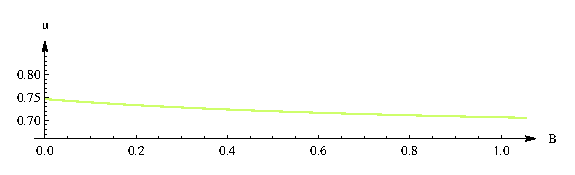
\includegraphics[width=0.9\textwidth]{C:/Users/BibiKiBa/Diss/Doktorarbeit/ModellEins/Abbildungen/uEL.eps}
\\
\hfill\footnotesize\sffamily{\textbf{Quelle:}}  eigene Darstellung
	\caption{Abh�ngigkeit des Anteils Humankapital $u$ im Produktionssektor einer relativ weniger weit entwickelten Volkswirtschaft von dem Offenheitsgrad $\bar{B}$}
	\label{fig:Ver�nderungHumankapitalOffenheitEL}
\end{figure}
\\
Das zus�tzliche technologische Wissen durch den Import von relativ humankapitalreicheren G�tern f�hrt zu einer Umverteilung des Humankapitalbestandes auf die beiden Sektoren Konsumg�terproduktion und Bildung. Mit steigender Offenheit, werden mehr G�ter importiert, von denen technologisches Wissen absorbiert werden kann. Dementsprechend wird der Bildungssektor in einem weniger weit, jedoch ge�ffnetem Land produktiver und die Haushalte werden mehr Humankapital in den Bildungssektor investieren, als in den Konsumgutsektor. Dementsprechend sinkt mit steigender Offenheit der Parameter $u$, wie aus Abbildung \ref{fig:Ver�nderungHumankapitalOffenheitEL} entnommen werden kann.\\
Ein �hnlicher Zusammenhang wird in Abbildung \ref{fig:ChiEL} dargestellt. Je st�rker sich ein Land �ffnet, oder je eher es Freihandel zul�sst, desto h�her ist die Konsum-Kapitalquote, die den optimalen Wachstumspfad bedingt. 
%ABBILDUNG \\
\begin{figure}[htb] 
\vspace{0.23cm}
 \centering 
 \psfrag{B}{$\bar{B}$}
		\psfrag{Chi}{$\chi$}
		\psfrag{0.0}[c]{\footnotesize{0}}
		\psfrag{0.2}[c]{\footnotesize{0.2}}
		\psfrag{0.4}[c]{\footnotesize{0.4}}
		\psfrag{0.6}[c]{\footnotesize{0.6}}
		\psfrag{1.2}[c]{\footnotesize{1.2}}
		\psfrag{1.4}[c]{\footnotesize{1.4}}
		\psfrag{1.6}[c]{\footnotesize{1.6}}
		\psfrag{0.8}[c]{\footnotesize{0.8}}
		%\psfrag{0.80}[l]{\footnotesize{0.8}}
		%\psfrag{0.9}[]{\footnotesize{0.9}}
		\psfrag{1.0}[c]{~\footnotesize{1.0}}
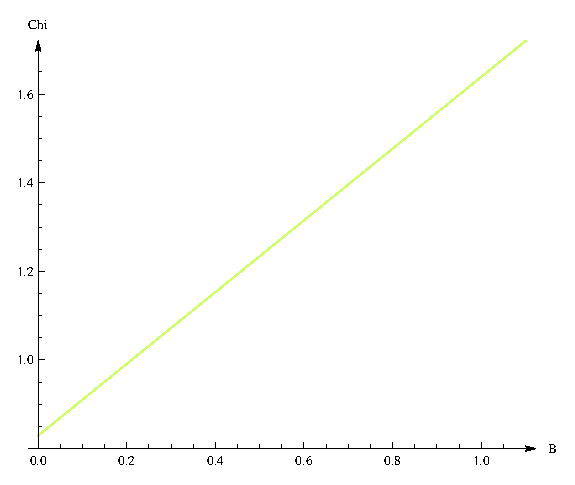
\includegraphics[width=0.54\textwidth]{C:/Users/BibiKiBa/Diss/Doktorarbeit/ModellEins/Abbildungen/ChiEL.eps}
\\
\hfill\footnotesize\sffamily{\textbf{Quelle:}}  eigene Darstellung
	\caption{Abh�ngigkeit der Kapital-Konsumquote $\chi$ einer relativ weniger weit entwickelten Volkswirtschaft von dem Offenheitsgrad $\bar{B}$}
	\label{fig:ChiEL}
\end{figure}
\\
Unter Ber�cksichtigung dieser berechneten optimalen Werte ergibt sich das gleichgewichtige Wirtschaftswachstum, das auch als Keynes-Ramsey-Regel bezeichnet wird. 
\begin{equation}
\boxed{\hat{c}^*=\frac{1}{\sigma}\left(\frac{1}{\alpha} B(1+\bar{B})-\rho\right)}
\end{equation}
Auch hier wird der positive Einfluss des Offenheitsparameters deutlich. Insgesamt wird die Wachstumsrate einer weniger weit entwickelten Volkswirtschaft durch Au{\ss}enhandel ansteigen, siehe Abbildung \ref{fig:cDachEL}.  
%ABBILDUNG 
\begin{figure}[htb] 
\vspace{0.23cm}
 \centering 
 \psfrag{B}{$\bar{B}$}
		\psfrag{cDach}{$\hat{c}$}
		\psfrag{0.0}[c]{\footnotesize{0}}
		\psfrag{0.2}[c]{\footnotesize{0.2}}
		\psfrag{0.4}[c]{\footnotesize{0.4}}
		\psfrag{0.6}[c]{\footnotesize{0.6}}
		\psfrag{0.9}[c]{\footnotesize{0.9}}
		\psfrag{0.7}[l]{\footnotesize{0.7}}
		\psfrag{0.75}[l]{\footnotesize{0.75}}
		\psfrag{0.8}[l]{\footnotesize{0.8}}
		%\psfrag{0.80}[l]{\footnotesize{0.8}}
		\psfrag{0.9}[l]{\footnotesize{0.9}}
		\psfrag{1.0}[l]{~\footnotesize{1}}
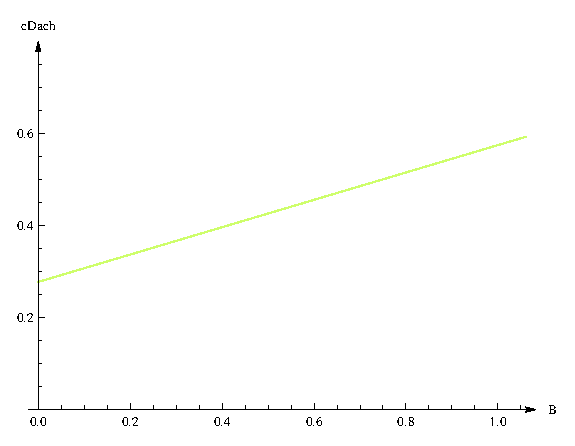
\includegraphics[width=0.54\textwidth]{C:/Users/BibiKiBa/Diss/Doktorarbeit/ModellEins/Abbildungen/cDachEL.eps}
\\
\hfill\footnotesize\sffamily{\textbf{Quelle:}}  eigene Darstellung
	\caption{Abh�ngigkeit der Wachstumsrate $\hat{c}$ einer relativ weniger weit entwickelten Volkswirtschaft von dem Offenheitsgrad $\bar{B}$}
	\label{fig:cDachEL}
\end{figure}

\FloatBarrier
\subsection{Handel in einem relativ weiter entwickelten Land}
Wird jetzt ein anderes Szenario betrachtet und von einem Land ausgegangen, dass relativ zum Weltmarkt weiter entwickelt ist, kann auch hier der Einfluss von Au{\ss}enhandel auf die intertemporale Konsumentscheidung gezeigt werden. Der Entwicklungsstand l�sst sich aus der relativen Ausstattung des Sachkapitals zum Humankapital herleiten. Das Grenzprodukt im Bildungssektor eines weiter entwickelten Landes ist h�her als das des relativ weniger weit entwickelten Weltmarktes. Somit gilt grunds�tzlich, dass tendenziell mehr Humankapital akkumuliert wird und beide Produktionsfaktoren im Bildungssektor verwendet werden. In einem sehr weit entwickelten Land werden bei der Ausbildung von Schneidern nicht nur die Lehrkraft als Humankapital eingesetzt, sondern auch die N�hmaschinen als Sachkapital. Ebenfalls denkbar w�re eine Schulung �ber Medien wie Tablets, die mittels Videos die zu erlernenden F�higkeiten verbreiten.\\ Ein relativ weiter entwickeltes Land verf�gt demnach �ber relativ mehr Humankapital als Sachkapital, verglichen mit dem weniger weit entwickelten Land oder auch Weltmarkt. Es ergibt sich demnach die Bewegungsgleichung f�r das physische Kapital:
\begin{equation}
\dot{k}(t)=A(v(t)k(t))^\alpha(u(t)h(t))^{1-\alpha}-c(t)-c_{ex}(t)+p^*c_{im}(t)
\end{equation}
Das physische Kapital ver�ndert sich �ber die Zeit, dahingehend, dass von dem produzierten G�termengen gem�{\ss} $y=A(v(t)k(t))^\alpha(u(t)h(t))^{1-\alpha}$ und den bewerteten importierten G�termengen $p^*c_{im}(t)$ die konsumierten G�ter des Inlandes $c(t)$ sowie die exportierten G�ter $c_{ex}(t)$ f�r das Ausland abgezogen werden. Die Kapitalakkumulation unterscheidet sich vom relativ weniger weit entwickelten Land nur durch den Faktor $v$, der den Anteil des Humankapitals bestimmt, der im Konsumgutsektor f�r die Produktion eingesetzt wird.\\   
Wie bereits angef�hrt, wird angenommen, dass in einem relativ weiter entwickelten Land f�r die Bildung neben Humankapital auch physisches Kapital eingesetzt wird.
\begin{equation}
\dot{h}(t)=B(1+\bar{B})((1-v(t))k(t))^{\eta}((1-u(t))h(t))^{1-\eta}
\end{equation}
Humankapital wird hier prinzipiell genauso akkumuliert, wie auf dem Weltmarkt, bzw. in der geschlossenen Referenzsituation, unter Ber�cksichtigung beider Kapitalarten. Demzufolge entwickelt sich das Humankapital �ber die Zeit, durch den Einsatz von Humankapital mit $((1-u(t))h(t))^{1-\eta}$ und von physischem Kapital mit $((1-v(t))k(t))^{\eta}$. Au{\ss}erdem beeinflussen auch hier die beiden Produktivit�tsparameter $B$ und $\bar{B}$ den Bildungssektor.\footnote{Der Offenheitsparameter verh�lt sich ebenso wie in \eqref{Offenheit}.} Auch hier wird k�nftig wieder auf die Notation der Abh�ngigkeit der Variablen gegen�ber der Zeit $t$ verzichtet.\\
Aus den Bewegungsgleichungen lassen sich die Wachstumsraten beider Kapitalarten herleiten: 
\begin{equation}
\hat{k}=Av^\alpha k^{\alpha-1}(uh)^{1-\alpha}-\frac{c}{k}-\frac{c_{ex}}{k}+p^*\frac{c_{im}}{k}\label{kHut}
\end{equation}
\begin{equation}
\hat{h}=B(1+\bar{B})\left[(1-v)\frac{k}{h}\right]^{\eta}(1-u)^{1-\eta}
\end{equation}
Die Relationen des physischen Kapitals zur Konsummenge lassen sich hier wieder verk�rzt darstellen als $\chi=\frac{c}{k}$, $\chi_{ex}=\frac{c_{ex}}{k}$ sowie $\chi_{im}=\frac{c_{im}}{k}$. Eingesetzt in \eqref{kHut} ergibt sich zun�chst:
\begin{equation}
\hat{k}=Av^\alpha u^{1-\alpha}\left(\frac{k}{h}\right)^{\alpha-1}-\chi-\chi_{ex}+p^*\chi_{im}
\end{equation}
Durch die Substitution von $x_1=\frac{vk}{uh}$ und $x_2=\frac{(1-v)k}{(1-u)h}$ lassen sich die Wachstumsraten wieder verk�rzt darstellen.\\ 
\begin{equation}
\boxed{\hat{k}=Ax_1^\alpha \frac{uh}{k}-\chi-\chi_{ex}+p^*\chi_{im}}
\end{equation}
\begin{equation}
\boxed{\hat{h}=B(1+\bar{B})x_2^\eta(1-u)}
\end{equation}
Erneut wird das Maximierungsproblem mit der Hamiltonfunktion, dem Maximumprinzip, gel�st. Es soll der optimale Konsumpfad gefunden werden, der den Lebenszeitnutzen eines Individuums maximiert, der in einer relativ weiter entwickelten Volkswirtschaft lebt, die handelsoffen ist.
\begin{equation}
\begin{split}
\mathbb{H}=&~e^{-\rho t}\frac{(c^\beta c_{im}^{1-\beta})^{1-\sigma}}{1-\sigma}\\
&+\gamma_1(A(vk)^\alpha(uh)^{1-\alpha}-c-c_{ex}+p^*c_{im})\\
&+\gamma_2B(1+\bar{B})[(1-v)k]^{\eta}[(1-u)h]^{1-\eta}\\
\end{split}
\end{equation}
Beschrieben wird dieser Konsumpfad durch folgendes Gleichungssystem: 
\begin{align}
&\frac{\partial\mathbb{H}}{\partial c}\overset{!}{=}~0\label{eq:lfoc1IL}\\
&\frac{\partial\mathbb{H}}{\partial c_{im}}\overset{!}{=}~0\label{eq:lfoc1imIL}\\
&\frac{\partial\mathbb{H}}{\partial v}\overset{!}{=}~0\label{eq:lfoc2IL}\\
&\frac{\partial\mathbb{H}}{\partial k}\overset{!}{=}-\dot{\gamma_1}\label{eq:lfoc3IL}\\
&\frac{\partial\mathbb{H}}{\partial k}\overset{!}{=}-\dot{\gamma}_{1im}\label{eq:lfoc3imIL}\\
&\frac{\partial\mathbb{H}}{\partial u}\overset{!}{=}~0\label{eq:lfoc4IL}\\
&\frac{\partial\mathbb{H}}{\partial h}\overset{!}{=}-\dot{\gamma_2}\label{eq:lfoc5IL}
\end{align}
Die Bedingungen des relativ weiter entwickelten Landes �hneln den beiden zuvor beschriebenen Zust�nden auf unterschiedliche Art und Weise. Die �hnlichkeit zur Referenzsituation ist gegeben, da hier das Humankapital auf die gleiche Art akkumuliert wird. Dem relativ weniger weit entwickelten Land �hnelt der Wachstumspfad, da es sich bei beiden um offene Volkswirtschaften handelt und somit die Offenheitsparameter diesen beeinflussen. Die ausf�hrliche Berechnung der Bedingungen erster Ordnung ist wieder in Appendix \ref{APPENDIXIL} zu finden. Zusammenfassend befindet sich eine relativ weiter entwickelte Volkswirtschaft dann im Gleichgewicht, wenn folgenden Restriktionen zutreffen.
\begin{align}
&\gamma_1=e^{-\rho t}\beta c^{\beta-1}c_{im}^{1-\beta}(c^\beta c_{im}^{1-\beta})^{-\sigma}\label{eq:foc1IL}\\
&\gamma_{1im}=-e^{-\rho t}(1-\beta) c^{\beta}c_{im}^{-\beta}(c^\beta c_{im}^{1-\beta})^{-\sigma}\label{eq:foc1imIL}\\
&\gamma_1A\alpha v^{\alpha-1}k^\alpha(uh)^{1-\alpha}=\gamma_2B(1+\bar{B})\eta(1-v)^{\eta-1}k^\eta[(1-u)h]^{1-\eta}\label{eq:foc2IL}\\
&\gamma_{1}A\alpha v^{\alpha} k^{\alpha -1} (u h)^{1- \alpha} + \gamma_{2}B(1+\bar{B})(1- v)^{\eta} k^{\eta -1} \eta \left [ (1-u)h \right ]^{1- \eta}= - \dot{\gamma}_{1}\label{eq:foc3IL}\\
&\gamma_{1 im}A\alpha v^{\alpha}k^{\alpha -1}(uh)^{1- \alpha}+ \gamma_{2}B(1+\bar{B}) [h(1-u)]^{1- \eta} \eta(1-v)^{\eta}k^{\eta -1}= - \dot{\gamma}_{1im}\label{eq:foc3imIL}\\
&\gamma_1A(1-\alpha)(vk)^{\alpha}u^{-\alpha}h^{1-\alpha}=\gamma_2B(1+\bar{B})(1-\eta)[(1-v)k]^\eta (1-u)^{-\eta} h^{1-\eta}\label{eq:foc4IL}\\
&\gamma_1A(1-\alpha)(vk)^\alpha u^{1-\alpha}h^{-\alpha}+\gamma_2 B(1+\bar{B})(1-\eta)[(1-v)k]^{\eta}(1-u)^{1-\eta}h^{-\eta}=-\dot{\gamma}_2\label{eq:foc5IL}
\end{align}
\vspace{-0.6cm}
\begin{equation}
\lim_{t \to \infty}e^{-\rho t}\gamma_1k=0;\qquad \lim_{t \to \infty}e^{-\rho t}\gamma_{1im}k=0; \qquad \lim_{t \to \infty}e^{-\rho t}\gamma_2h=0
\end{equation}
Auch hier wird in Gleichung \eqref{eq:foc1IL} zun�chst der Schattenpreis einer zus�tzlichen Einheit Kapital beschrieben. Dieser daraus resultierende zuk�nftige Lebenszeitgrenznutzen muss dem gegenw�rtigen Nutzen entsprechen, der aus einer zus�tzliche konsumierten Einheit resultiert. Der gleiche Zusammenhang, jedoch auf das importierte Gut $c_{im}$ bezogen beschreibt Gleichung \eqref{eq:foc1imIL}.\\
Bedingung \eqref{eq:foc2IL} und Gleichung \eqref{eq:foc4IL} gew�hrleisten, dass eine Volkswirtschaft erst dann im Gleichgewicht ist, wenn sich die mit dem jeweiligen Schattenpreis bewerteten Grenzprodukte entsprechen.\\
Die verbleibenden drei Bedingungen \eqref{eq:foc3IL}, \eqref{eq:foc3imIL} und \eqref{eq:foc5IL} beschreiben jeweils die Abschreibungsrate des Schattenpreises. Die durch Au{\ss}enhandel im relativ weiter entwickelten Land h�her sind, als in der Referenzsituation ohne Handel. Der Nutzwert einer zus�tzlichen Kapitaleinheit ist somit h�her und muss damit auch �ber die Lebenszeit st�rker abgeschrieben werden. 

\subsubsection*{Modelldynamik}
Aus den angef�hrten Bedingungen lassen sich die Keynes-Ramsey-Regeln, also die Konsumwachstumsraten f�r das heimisch produzierte und das importierte Konsumgut herleiten. 
\begin{equation}
\boxed{
\hat{c}=\frac{1}{(1-\beta+\sigma\beta)}\left(A\alpha x_1^{\alpha -1}-\rho+\hat{c}_{im}(1-\beta+\sigma\beta-\sigma)\right)}
\end{equation}
\begin{equation}
\boxed{
\hat{c}_{im}=\frac{1}{\beta-\sigma\beta+ \sigma}\left(A\alpha x_1^{\alpha -1}-\rho+\hat{c}(\beta - \sigma\beta)\right)}
\end{equation}
Beide Wachstumsraten bedingen sich gegenseitig, denn je nach H�he der Konsum\-g�ter\-einfuhr kann weniger von den inl�ndisch produzierten G�tern konsumiert werden und umgekehrt.\\
Ebenso wie in der Autarkiesituation entsprechen sich die Verh�ltnisse der Grenzproduktivit�ten beider Sektoren.\footnote{Die Herleitung folgt aus den Gleichungen \eqref{eq:foc2IL} und \eqref{eq:foc3IL}, siehe dazu Appendix \ref{APPENDIXIL}.}
\begin{equation}
\boxed{\frac{1-\alpha}{\alpha}x_1=\frac{1-\eta}{\eta}x_2}
\end{equation}
In diesem Fall beeinflusst der Au{\ss}enhandel die Grenzproduktivit�ten nicht. Die Grenzproduktivit�t einer marginalen Ver�nderung des Sach- oder Humankapitals im Konsumgutsektor sowie im Bildungssektor entsprechen sich, unabh�ngig von internationalen Einfl�ssen.\\
Dass die Wachstumsrate des Schattenpreises des physischen Kapitals dem Grenzprodukt des Kapitals entspricht, wird ist in der folgenden Gleichung formuliert. 
\begin{equation}\boxed{
B(1+\bar{B})(1-\eta)x_2^\eta=-\rho-\hat{c}(\beta-1-\sigma\beta)-\hat{c}_{im}(1-\beta+\sigma\beta-\sigma)-\alpha\hat{x}_1+\eta\hat{x}_2}
\end{equation}
Diese Schreibweise zeigt den Einfluss des Importg�terwachstums, sofern noch kein Au{\ss}enhandelsgleichgewicht angenommen wird, auf das Grenzprodukt des Kapitals im Konsumgutsektor. Das Grenzprodukt des Humankapitals im Bildungssektor ist aufgrund der Handelsbeziehungen, hier abgebildet durch den Offenheitsgrad $\bar{B}$, h�her als in der Autarkiesituation. Beide Grenzprodukte und somit auch die Lebenszeitgrenznutzenwachstumsrate entsprechen sich auch in einer offenen Volkswirtschaft.
Der optimale Wachstumspfad eines offenen relativ weiter entwickelten Landes wird durch das folgende Gleichungssystem beschrieben. 
\begin{align}
&\hat{k}=Ax_1^\alpha \frac{uh}{k}-\chi-\chi_{ex}+p^*\chi_{im}\\
&\hat{h}=B(1+\bar{B})x_2^\eta(1-u)\\
& x_1(1-\alpha)/\alpha =x_2(1-\eta)/\eta\\
&\hat{c}=\frac{1}{(1-\beta+\sigma\beta)}\left(A\alpha x_1^{\alpha -1}-\rho+\hat{c}_{im}(1-\beta+\sigma\beta-\sigma)\right)\\
&\hat{c}_{im}=\frac{1}{\beta-\sigma\beta+ \sigma}\left(A\alpha x_1^{\alpha -1}-\rho+\hat{c}(\beta - \sigma\beta)\right)\\
&B(1+\bar{B})(1-\eta)x_2^\eta=-\rho-\hat{c}(\beta-1-\sigma\beta)-\hat{c}_{im}(1-\beta+\sigma\beta-\sigma)-\alpha\hat{x}_1+\eta\hat{x}_2
\end{align}
F�r die Bestimmung des Gleichgewichts sind jedoch auch hier die einzelnen Werte zu berechnen. F�r die exakte Berechnung aller weiteren Variablen werden die gleichgewichtigen Relationen $x_1$ und $x_2$ ben�tigt, dessen Wachstum konstant ist,  
\colorbox{lightgray}{$\hat{x}_1=\hat{x}_2=0$}. Aus dem Gleichungssystem ergibt sich: 
\begin{equation}
x_2^*=\left(\frac{\rho+\sigma\hat{c}}{B(1+\bar{B})(1-\eta)}\right)^{1/\eta}
\end{equation}
\begin{equation}
x_1^* =\frac{\alpha(1-\eta)}{\eta(1-\alpha)}\left(\frac{\rho+\sigma\hat{c}}{B(1+\bar{B})(1-\eta)}\right)^{1/\eta}
\end{equation}
Wird davon ausgegangen, dass sich die Volkswirtschaft auch im Au{\ss}enhandelsgleichgewicht befindet, dann entsprechen sich beide Konsumg�terwachstumsraten \colorbox{lightgray}{$\hat{c}=\hat{c}_{im}$}. 
\begin{equation}
\hat{c}=\frac{1}{\sigma}(A\alpha x_1^{\alpha-1}-\rho)
\end{equation}
Daraus ergibt sich das gleichgewichtige Konsumwachstum einer ge�ffneten Volkswirtschaft eines relativ weiter entwickelten Landes, das sich hinsichtlich des Offenheitsparameter $\bar{B}$ von der hiesigen im Autarkiezustand unterscheidet.
\begin{equation}
\boxed{\hat{c}^*=\frac{1}{\sigma}\left(\left[A^\eta\alpha^{\alpha\eta}(1-\eta)^{(1-\eta)(1-\alpha)}(\eta(1-\alpha))^{\eta(1-\alpha)}(B(1+\bar{B}))^{1-\alpha}\right]^\frac{1}{1+\eta-\alpha}-\rho\right)}
\end{equation}
Je offener eine Volkswirtschaft ist und desto mehr technisches Wissen durch den Import von G�tern absorbiert werden kann, desto h�her ist die Wachstumsrate.\footnote{In diesem Abschnitt wird das Grenzprodukt der �bersichtlichkeit halber verk�rzt durch $\bar{M}=\left[A^\eta\alpha^{\alpha\eta}(1-\eta)^{(1-\eta)(1-\alpha)}(\eta(1-\alpha))^{\eta(1-\alpha)}(B(1+\bar{B}))^{1-\alpha}\right]^\frac{1}{1+\eta-\alpha}$} Dieser Zusammenhang ist auch der folgenden Abbildung \ref{fig:cDachIL} zu entnehmen. 
%ABBILDUNG 
\begin{figure}[htb] 
\vspace{0.23cm}
 \centering 
 \psfrag{B}{$\bar{B}$}
		\psfrag{cDAch}{$\hat{c}$}
		\psfrag{0.0}[c]{\footnotesize{0}}
		\psfrag{0.2}[c]{\footnotesize{0.2}}
		\psfrag{0.4}[c]{\footnotesize{0.4}}
		\psfrag{0.6}[c]{\footnotesize{0.6}}
		\psfrag{0.05}[c]{\footnotesize{0.05}}
		\psfrag{0.10}[c]{\footnotesize{0.10}}
		\psfrag{0.15}[c]{\footnotesize{0.15}}
		\psfrag{0.8}[l]{\footnotesize{0.8}}
		%\psfrag{0.80}[l]{\footnotesize{0.8}}
		\psfrag{0.9}[l]{\footnotesize{0.9}}
		\psfrag{1.0}[l]{~\footnotesize{1}}
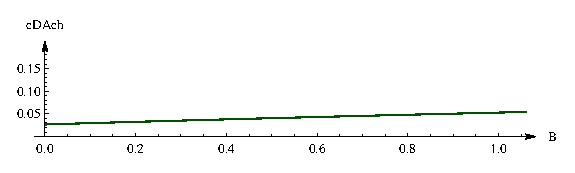
\includegraphics[width=0.9\textwidth]{C:/Users/BibiKiBa/Diss/Doktorarbeit/ModellEins/Abbildungen/cDachIL.eps}
\\
\hfill\footnotesize\sffamily{\textbf{Quelle:}}  eigene Darstellung
	\caption{Abh�ngigkeit der Wachstumsrate $\hat{c}$ einer relativ weiter entwickelten Volkswirtschaft von dem Offenheitsgrad $\bar{B}$}
	\label{fig:cDachIL}
\end{figure}
\\
Auch hier wird die gleichgewichtige optimale Aufteilung des Kapitals auf die beiden Sektoren Bildung und Konsumg�terproduktion ermittelt, dadurch, dass die Rate des Humankapitalwachstums der des Konsumg�terwachstums entspricht, \colorbox{lightgray}{$\hat{c}=\hat{h}$}.
\begin{equation}
\boxed{u^*=\frac{\sigma \bar{M}-(1-\eta)(\bar{M}-\rho)}{\sigma \bar{M}}}
\end{equation}
Diese Gleichung zeigt, dass Au{\ss}enhandel in einem relativ weiter entwickelten Land �ber das Grenzprodukt $\bar{M}$ Einfluss auf die Entscheidung hat, weniger Humankapital in den Konsumg�tersektor zu investieren. Je mehr Technologietransfer durch steigende Offenheit $\bar{B}$ stattfindet, desto weniger Humankapital wird in den Produktionsprozess eingehen und daf�r den Bildungssektor unterst�tzen, aufgrund eines Anstiegs von $(1-u)$. Dieser Zusammenhang ist in Abbildung \ref{fig:Ver�nderungHumankapitalOffenheit} dargestellt.  \\%ABBILDUNG
\begin{figure}[htb!] 
\vspace{0.13cm}
 \centering 
 \psfrag{B}{$\bar{B}$}
		\psfrag{u}{  $u$}
		\psfrag{0.0}[l]{\footnotesize{0}}
		\psfrag{0.2}[l]{\footnotesize{0.2}}
		\psfrag{0.4}[l]{\footnotesize{0.4}}
		\psfrag{0.6}[l]{\footnotesize{0.6}}
		\psfrag{0.70}[l]{\footnotesize{0.7}}
		\psfrag{0.75}[l]{\footnotesize{0.75}}
		\psfrag{0.8}[l]{\footnotesize{0.8}}
		\psfrag{0.80}[l]{\footnotesize{0.80}}
		\psfrag{0.85}[l]{\footnotesize{0.85}}
		\psfrag{0.90}[l]{\footnotesize{0.90}}
		\psfrag{1.0}[l]{~\footnotesize{1}}
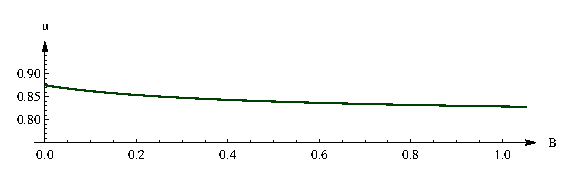
\includegraphics[width=0.9\textwidth]{C:/Users/BibiKiBa/Diss/Doktorarbeit/ModellEins/Abbildungen/uIL.eps}
\\
\hfill\footnotesize\sffamily{\textbf{Quelle:}}  eigene Darstellung
	\caption{Abh�ngigkeit des Anteils Humankapital $u$ im Produktionssektor einer relativ weiter entwickelten Volkswirtschaft von dem Offenheitsgrad $\bar{B}$}
	\label{fig:Ver�nderungHumankapitalOffenheit}
\end{figure}
\\
Nicht nur durch die Umverteilung des Humankapitals f�hrt Freihandel zum Anstieg qualifizierter Arbeitskr�fte, sondern es wird durch die Verteilung des Sachkapitals $v$ auf die beiden Sektoren auch das Bildungssystem gef�rdert. 
\begin{equation}
\boxed{
v^*=\frac{\alpha  (1-\eta ) \left(\frac{\bar{M}}{B (1+\bar{B}) (1-\eta )}\right)^{1/\eta } (\bar{M} \sigma -(1-\eta ) (\bar{M}-\rho ))}{(1-\alpha ) \eta  \bar{M} \sigma  \left(\frac{\alpha  (1-\eta ) \left(\frac{\bar{M}}{B (1+\bar{B}) (1-\eta )}\right)^{1/\eta } (\bar{M} \sigma -(1-\eta ) (\bar{M}-\rho ))}{(1-\alpha ) \eta  \bar{M} \sigma }+\left(\frac{\bar{M}}{B (1+\bar{B}) (1-\eta )}\right)^{1/\eta } \left(1-\frac{\bar{M} \sigma -(1-\eta ) (\bar{M}-\rho )}{\bar{M} \sigma }\right)\right)}}
\end{equation}
Ebenso verh�lt es sich mit der Aufteilung des Sachkapitals. Auch hier wirkt die Offenheit im Grenzprodukt als prim�rer Einflussfaktor zugunsten des Bildungssektors.\\ Abbildung \ref{fig:Ver�nderungSachkapitalOffenheit} stellt die negative Abh�ngigkeit des auf den Konsumgutsektor entfallenden Anteil des Sachkapitals $v$ zu der Offenheit dar. 
%ABBILDUNG
\begin{figure}[htb] 
\vspace{0.13cm}
 \centering 
 \psfrag{B}{$\bar{B}$}
		\psfrag{v}{  $v$}
		\psfrag{-}{  $_-$}
		\psfrag{1}{\, $_1$}
		\psfrag{0.0}[l]{\footnotesize{0}}
		\psfrag{0.2}[l]{\footnotesize{0.2}}
		\psfrag{0.4}[l]{\footnotesize{0.4}}
		\psfrag{0.6}[l]{\footnotesize{0.6}}
		\psfrag{0.70}[l]{\footnotesize{0.70}}
		\psfrag{0.75}[l]{\footnotesize{0.75}}
		\psfrag{0.8}[l]{\footnotesize{0.8}}
		\psfrag{0.80}[l]{\footnotesize{0.80}}
		\psfrag{1.0}[l]{~\footnotesize{1}}
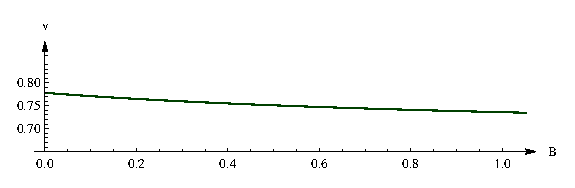
\includegraphics[width=0.9\textwidth]{C:/Users/BibiKiBa/Diss/Doktorarbeit/ModellEins/Abbildungen/vIL.eps}
\\
\hfill\footnotesize\sffamily{\textbf{Quelle:}}  eigene Darstellung
	\caption{Abh�ngigkeit des Anteils Sachkapital $v$ im Produktionssektor einer relativ weiter entwickelten Volkswirtschaft von dem Offenheitsgrad $\bar{B}$}
	\label{fig:Ver�nderungSachkapitalOffenheit}
\end{figure}
\\
Au{\ss}erdem ist es notwendig, dass die Kapital-Konsumquote $\chi$ im Gleichgewicht konstant ist. Dies gilt immer dann, wenn \colorbox{lightgray}{$\hat{c}=\hat{k}$} im Gleichgewicht gilt und ist ebenfalls abh�ngig vom Diffusionsparameter $\bar{B}$, siehe Abbildung \ref{fig:ChiIL}.
\begin{equation}
\boxed{\chi^*=\frac{1}{\sigma}\left(\frac{A\alpha \sigma[-\eta\rho+\bar{M}(\eta+\sigma-1)+\rho] \left(\frac{\alpha  (\eta -1) \left(\frac{\bar{M}}{B (1+\bar{B})(1-\eta) }\right)^{1/\eta }}{(\alpha -1) \eta }\right)^{\alpha -1}}{\rho  (\alpha -\eta )+\bar{M} (\alpha  (\sigma -1)+\eta )}-\bar{M}+\rho\right)}
\end{equation}
%ABBILDUNG 
\begin{figure}[h!] 
\vspace{0.23cm}
 \centering 
 \psfrag{B}{$\bar{B}$}
	\psfrag{Chi}{$\chi$}
		\psfrag{0.0}[c]{\footnotesize{0}}
		\psfrag{0.2}[c]{\footnotesize{0.2}}
		\psfrag{0.4}[l]{\footnotesize{0.4}}
		\psfrag{0.6}[l]{\footnotesize{0.6}}
		\psfrag{0.3}[l]{\footnotesize{0.3}}
		\psfrag{0.10}[c]{\footnotesize{0.10}}
		\psfrag{0.5}[l]{\footnotesize{0.5}}
		\psfrag{0.8}[c]{\footnotesize{0.8}}
		%\psfrag{0.80}[l]{\footnotesize{0.8}}
		\psfrag{0.9}[c]{\footnotesize{0.9}}
		\psfrag{1.0}[c]{~\footnotesize{1}}
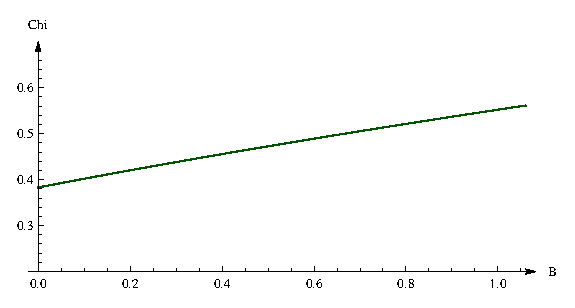
\includegraphics[width=0.9\textwidth]{C:/Users/BibiKiBa/Diss/Doktorarbeit/ModellEins/Abbildungen/ChiIL.eps}
\\
\hfill\footnotesize\sffamily{\textbf{Quelle:}}  eigene Darstellung
	\caption{Abh�ngigkeit der Kapital-Konsumquote $\chi$ einer relativ weiter entwickelten Volkswirtschaft von dem Offenheitsgrad $\bar{B}$}
	\label{fig:ChiIL}
\end{figure}

\subsection{Handelspolitik}
Bisher wurde nicht immer von der Offenheit eines Landes gesprochen ohne dabei auch die wohlfahrtsmindernde Wirkung protektionistischer Ma{\ss}nahmen zu ber�cksichtigen. Eingangs bei der Betrachtung des Offenheitsparameter $\bar{B}$ wurde impliziert, dass dieser geringer ist, wenn das Handelsvolumen kleiner ist. Dieses kleinere Handelsvolumen kann aus der aktiven Einschr�nkung des Handels durch Z�lle, Kontingente, Subventionen oder auch nicht- tarif�ren Handelshemmnissen wie Richtlinien resultieren. Bei der folgenden Zusammenfassung des Einflusses von Au{\ss}enhandel auf den Entwicklungsprozess, kann somit zugleich von einer gegens�tzlichen Wirkung von Handelshemmnissen ausgegangen werden. 
%\textcolor[rgb]{1,0,0}{(so drin lassen??? kommt in Kapitel Papier 1 nochmal handelshemmnis? ist diese Exportf�rderung ein Hemmnis???) }

\section{Zwischenfazit}
In diesem Kapitel wurde der Einfluss von Au{\ss}enhandel auf die Humankapitalakkumulation bei unterschiedlichen Entwicklungsst�nden untersucht. Verdeutlicht werden die Ergebnisse anhand eines Vergleichs beider Szenarien mit der Referenzsituation Autarkie. Durch den Anteil des Sachkapitals der in der G�terproduktion aufgewendet wird $v$, k�nnen auch indirekt Aussagen �ber den Bildungssektor getroffen werden, da sich der Anteil des physischen Kapitals im Bildungssektor aus $(1-v)$ ergibt. Der Vergleich der verschiedenen Entwicklungsstadien ist in Abbildung \ref{fig:VergleichV} dargestellt. In einem relativ \textcolor[rgb]{0,0.58,0}{weiter entwickelten Land} sinkt $v$ mit zunehmender Offenheit. Aus der Perspektive des Bildungssektors stellt sich dieser mit der Zunahme der Offenheit besser, als wenn ein Land geschlossen ist, da nun mehr Sachkapital im Bildungssektor eingesetzt wird.\\  %ABBILDUNG
\begin{figure}[htb] 
\vspace{0.13cm}
 \centering 
 \psfrag{B}{$\bar{B}$}
		\psfrag{v}{  $v$}
		\psfrag{0.0}[l]{\footnotesize{0}}
		\psfrag{0.2}[l]{\footnotesize{0.2}}
		\psfrag{0.4}[l]{\footnotesize{0.4}}
		\psfrag{0.6}[l]{\footnotesize{0.6}}
		\psfrag{0.7}[l]{\footnotesize{0.7}}
		\psfrag{0.75}[l]{\footnotesize{0.75}}
		\psfrag{0.8}[l]{\footnotesize{0.8}}
		%\psfrag{0.80}[l]{\footnotesize{0.8}}
		\psfrag{0.9}[l]{\footnotesize{0.9}}
		\psfrag{1.0}[l]{~\footnotesize{1}}
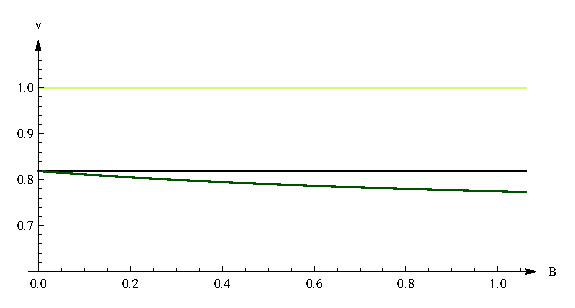
\includegraphics[width=0.9\textwidth]{C:/Users/BibiKiBa/Diss/Doktorarbeit/ModellEins/Abbildungen/VergleichV.eps}
\\
\hfill\footnotesize\sffamily{\textbf{Quelle:}}  eigene Darstellung
	\caption{Ver�nderung des Anteils Sachkapital $v$ im Produktionssektor unterschiedlicher Entwicklungsstadien abh�ngig von dem Offenheitsgrad $\bar{B}$}
	\label{fig:VergleichV}
\end{figure}
\\
Das Niveau der Entscheidungsvariablen $v$ der Haushalte aus \textcolor[rgb]{0.74,0.97,0.22}{weniger weit entwickelten L�ndern} ist deutlich h�her und konstant, da $v=1$. Somit wird das gesamte physische Kapital in die G�terproduktion eingehen. Durch den Verzicht des Einsatzes von physischem Kapital in den Bildungssektor, wird das Sachkapital komplett f�r die Produktion von G�tern verwendet und f�hrt dazu, dass im Konsumgutsektor insgesamt weniger Humankapital eingesetzt werden muss. Dadurch wird der Haushalt deutlich mehr Humankapital in Bildungssektor investieren. Dieser Zusammenhang kann der Abbildung \ref{fig:VergleichU} entnommen werden. %\\ABBILDUNG
\begin{figure}[htb] 
\vspace{0.13cm}
 \centering 
 \psfrag{B}{$\bar{B}$}
		\psfrag{u}{  $u$}
		\psfrag{0.0}[c]{\footnotesize{0}}
		\psfrag{0.2}[c]{\footnotesize{0.2}}
		\psfrag{0.4}[c]{\footnotesize{0.4}}
		\psfrag{0.6}[c]{\footnotesize{0.6}}
		\psfrag{0.9}[c]{\footnotesize{0.9}}
		\psfrag{0.7}[c]{\footnotesize{0.7}}
		\psfrag{0.75}[l]{\footnotesize{0.75}}
		\psfrag{0.8}[c]{\footnotesize{0.8}}
		%\psfrag{0.80}[l]{\footnotesize{0.8}}
		\psfrag{0.9}[c]{\footnotesize{0.9}}
		\psfrag{1.0}[c]{~\footnotesize{1}}
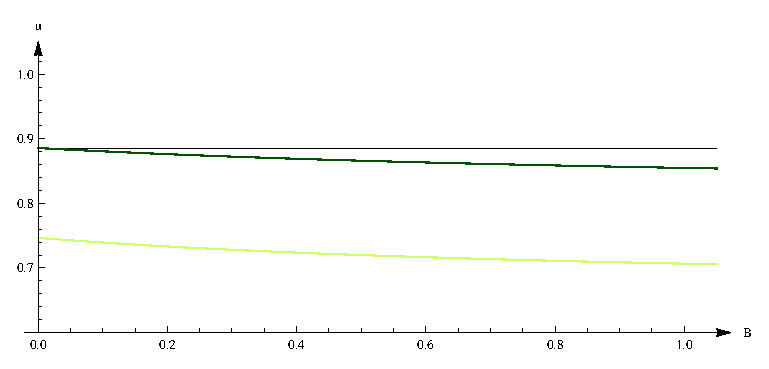
\includegraphics[width=0.9\textwidth]{C:/Users/BibiKiBa/Diss/Doktorarbeit/ModellEins/Abbildungen/VergleichU.eps}
\\
\hfill\footnotesize\sffamily{\textbf{Quelle:}}  eigene Darstellung
	\caption{Ver�nderung des Anteils Humankapital $u$ im Produktionssektor  unterschiedlicher Entwicklungsstadien abh�ngig von dem Offenheitsgrad $\bar{B}$}
	\label{fig:VergleichU}
\end{figure}
\\
Unabh�ngig von dem Entwicklungsstand kommt es immer zu einer Aufteilung des Humankapitals auf beide Sektoren. Durch Au{\ss}enhandel sinkt der Anteil des Humankapitals $u$, der in den Konsumgutsektor eingeht, demzufolge steigt der Anteil im Bildungssektor $(1-u)$ an. Jedoch gibt es auch hier Niveauunterschiede. In dem hier angef�hrten Beispiel werden die Haushalte eines \textcolor[rgb]{0.74,0.97,0.22}{weniger weit entwickelten Landes} ca. 25\% des Humankapitals von den Haushalten in den Bildungssektor einsetzen, dieser Anteil nimmt mit der �ffnung des Landes zu.\footnote{Da die relativ weniger weit entwickelten L�nder nur Humankapital in den Bildungssektor investieren, kann das Sachkapital vollst�ndig f�r die Konsumg�terproduktion verwendet werden. Demzufolge wird verh�ltnism�{\ss}ig weniger Humankapital (75\%) f�r die Produktion verwendet als in einem relativ weiter entwickelten Land (90\%). Der verbleibende h�here Anteil Humankapital kann nun zus�tzlich in den Bildungssektor investiert werden. Demzufolge resultiert der angesprochene Niveauunterschied.} Haushalte in \textcolor[rgb]{0,0.58,0}{relativ weiter entwickelten Volkswirtschaften} werden auch weniger Humankapital in die G�terproduktion investiert, daf�r aber immer mehr in den Bildungssektor je st�rker sich das Land �ffnet. Im Vergleich zur \textbf{Autarkiesituation} verbessert sich in beiden Situationen die Humankapitalakkumulation durch Freihandel. \\
Demzufolge entscheiden sich die Haushalte in ge�ffneten Volkswirtschaften zu Gunsten der eigenen Weiterbildung und gewichten somit das hinzugekommene technische Wissen st�rker  als in einer geschlossenen Volkswirtschaft. Freihandel kann ein Ansatz sein, die Anreize der Bev�lkerung zu erh�hen sich weiterzubilden, unabh�ngig vom Entwicklungsstand. \\
Die �ffnung eines Landes verst�rkt den Wissenstransfer und die damit einhergehende Technologiediffusion. Das Modell zeigt, dass der Humankapitalbestand in relativ weniger weit entwickelten Volkswirtschaften durch Au{\ss}enhandel ansteigt und dadurch die L�cke zur �brigen Welt geschlossen werden kann. Denn der Technologietransfer wird verst�rkt durch den Handel mit humankapitalreichen G�tern, die in das weniger weit entwickelte Land importiert werden. Dadurch steigt die Wachstumsrate dieses Landes an und konvergiert zum Weltmarktgleichgewicht. Diese Wirkung auf das Wirtschaftswachstum zeigt folgend die Abbildung \ref{fig:cDachVergleich}.  
%ABBILDUNG 
\begin{figure}[htb] 
\vspace{0.23cm}
 \centering 
 \psfrag{B}{$\bar{B}$}
		\psfrag{cDach}{$\hat{c}$}
		\psfrag{0.0}[c]{\footnotesize{0}}
		\psfrag{0.2}[c]{\footnotesize{0.2}}
		\psfrag{0.4}[c]{\footnotesize{0.4}}
		\psfrag{0.6}[c]{\footnotesize{0.6}}
		\psfrag{0.5}[c]{\footnotesize{0.5}}
		\psfrag{0.3}[c]{\footnotesize{0.3}}
		\psfrag{0.1}[c]{\footnotesize{0.1}}
		\psfrag{0.8}[c]{\footnotesize{0.8}}
		%\psfrag{0.80}[l]{\footnotesize{0.8}}
		\psfrag{0.9}[c]{\footnotesize{0.9}}
		\psfrag{1.0}[c]{~\footnotesize{1}}
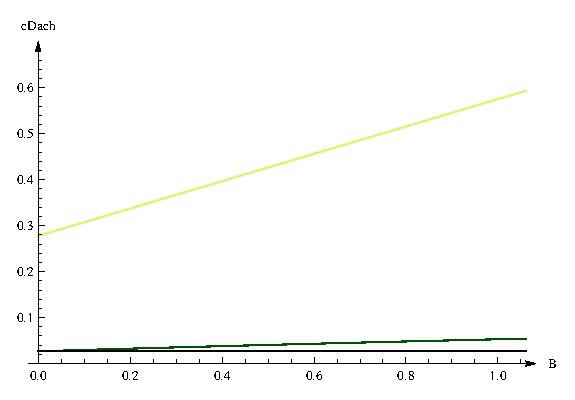
\includegraphics[width=0.7\textwidth]{C:/Users/BibiKiBa/Diss/Doktorarbeit/ModellEins/Abbildungen/cDachVergleich.eps}
\\
\hfill\footnotesize\sffamily{\textbf{Quelle:}}  eigene Darstellung
	\caption{Vergleich der Wachstumsraten $\hat{c}$ unterschiedlicher Entwicklungsstadien abh�ngig von dem Offenheitsgrad $\bar{B}$}
	\label{fig:cDachVergleich}
\end{figure}
\\
Die Referenzsituation einer \textbf{geschlossenen Volkswirtschaft} zeigt keine Abh�ngigkeit des Wirtschaftswachstums gegen�ber der Offenheit. Die Produktionsstrukturen eines \textcolor[rgb]{0,0.58,0}{relativ weiter entwickelten Landes} sind denen der hier aufgef�hrten Autarkiesituation sehr �hnlich, da bei beiden $v>0$ gilt. Demzufolge ist das Wirtschaftswachstum beider Situationen einer geschlossenen Volkswirtschaft mit $\bar{B}=0$ noch gleich. Das offene relativ weiter entwickelte Land verzeichnet jedoch mit zunehmender Offenheit einen geringen Anstieg der Wachstumsrate.\\
Das \textcolor[rgb]{0.74,0.97,0.22}{weniger weit entwickelte Land} startet von einem deutlich h�heren Wert der Wachstumsrate $\hat{c}$ bei $\bar{B}=0$ und verzeichnet noch eine st�rkere Zunahme der Wachstumsrate mit steigender Offenheit $\bar{B}$. Dieser recht steile Anstieg spiegelt den Aufholprozess weniger weit entwickelter L�nder wieder. Die Ver�nderung des Grenzproduktes ist in weniger weit entwickelten Volkswirtschaften noch h�her und f�hrt somit auch zu einer h�heren Wachstumsrate. Hinzu kommt, dass der Wissenstransfer f�r ein weniger weit entwickeltes Land deutlich h�her ist und Wissen aufholen kann, als ein relativ weiter entwickeltes Land.\\
Im Ergebnis zeigt diese Abbildung, dass unabh�ngig vom Entwicklungsstand und den damit einhergehenden Bildungssystemen Freihandel zu einer h�heren Wachstumsrate f�hrt. \\
In dem folgenden Kapitel wird ein Modell vorgestellt, dass den technischen Fortschritt beschreibt und das hier akkumulierte Humankapital zu Imitationen bzw. Innovationen umwandelt. Die Anwendung, Implementierung und Entwicklung neuer Technologien ben�tigt qualifizierte Arbeit. So best�tigen auch \citet{Nelson.1966} die Bedeutung des Humankapital f�r den technischen Fortschritt einer Volkswirtschaft. Ein hoher Bildungsstand beschleunigt den Prozess der technischen Diffusion und, dass demzufolge eher Innovationen entwickelt werden. Daraus l{\"a}sst sich f{\"u}r diese Arbeit der R�ckschluss ziehen, dass hohe Qualifikationen der Unternehmer f{\"u}r die Entwicklung von Innovationen notwendig sind und sich daraufhin f{\"u}r eine passende Strategie entschieden wird. Das folgende Modell wird daher die Bedeutung von F{\"a}higkeiten und Humankapital f{\"u}r die passende Entscheidung bez�glich einer Unternehmensstrategie und auch f{\"u}r den technischen Fortschritt betonen.

%\end{document}
%
\chapter{Auswertung}\label{Auswertung}

In Bezug auf die in Kapitel \ref{Einleitung} aufgestellten Thesen zeigt die vorangegangene Analyse, dass Au{\ss}enhandel die Bedeutung des Humankapitals f{\"u}r den Wachstumsprozess betont. In einem weiteren Schritt wurde gezeigt, dass nicht nur Humankapital per se wichtig ist, sondern auch seine Zusammensetzung,  bezogen auf heterogene F{\"a}higkeit, der imitierenden und innovierenden Art. Au{\ss}enhandel stimuliert die Innovationsf{\"a}higkeit von Volkswirtschaften und best{\"a}tigt zudem, dass abh{\"a}ngig vom Entwicklungsstand auch die Imitationsstrategie den Entwicklungsprozess voranbringt. Es wurde gezeigt, dass Freihandel durch eine entsprechende Strategiewahl die Entwicklung aller L{\"a}nder beg{\"u}nstigt, unabh{\"a}ngig vom Entwicklungsstand und der Beschaffenheit der Welttechnologiegr{\"o}{\ss}e. Technologisch kleine sowie technologisch gro{\ss}e L{\"a}nder profitieren vom Wissenstransfer und ebnen damit die M{\"o}glichkeit f{\"u}r dauerhaftes Wachstum.\\


Es konnte gezeigt werden, dass weniger weit entwickelte L{\"a}nder vom Handel mit relativ humankapitalreich produzierten G{\"u}tern profitieren und sich dadurch ihr eigenes Bildungswesen verbessert. Diese Anhebung des Bildungsniveaus eines Landes f{\"u}hrt zu einem h{\"o}heren Wachstumspfad, durch die Weiterentwicklung des technologischen Entwicklungsstands. So bewirkt Au{\ss}enhandel mit humankapitalreichen G{\"u}tern, dass relativ weiter entwickelte L{\"a}nder die Innovationsstrategie verfolgen und relativ weniger weit entwickelte die Imitationsstrategie.\footnote{Je nach N{\"a}he zur WTG k{\"o}nnte jedoch ein Wechsel angeraten werden.} Unabh{\"a}ngig von der technologischen Gr{\"o}{\ss}e des Landes resultiert das gleiche Ergebnis. Demzufolge wird auch bei technologisch gro{\ss}en L{\"a}ndern, die eine endogene WTG bedingen, mit abnehmender Distanz zur WTG die Innovationsstrategie pr{\"a}feriert. Der Abstand zur WTG wird sich zwar ausweiten, jedoch f{\"u}hrt Au{\ss}enhandel zu einem absolut gesehen zuk{\"u}nftig h{\"o}heren Entwicklungsstand.\footnote{In der folgenden Auswertung wird nicht mehr zwischen den Ergebnissen bei einer endogenen und exogenen WTG unterschieden, da dies keinen wesentlichen Einfluss auf die strategische Entscheidung eines Landes hat.}\newline


Differenziert man zus{\"a}tzlich zwischen den Sektoren, was aus der exportunterst{\"u}tzenden Politik folgte\footnote{Diese wurde in Kapitel \ref{Papier1} modelliert.}, dann zeigt dies ebenfalls, dass bei einem sehr hohen Abstand zur WTG durchaus die Imitationsstrategie im Importsektor zu pr{\"a}ferieren ist. Dies sollte einer Volkswirtschaft dazu verhelfen eine Basis an technologischem Wissen und Humankapital aufzubauen, indem zun{\"a}chst Wissen importiert wird, das nun nachgeahmt werden kann, bevor ein Wechsel zur Innovationsstrategie sinnvoll ist. Dieser Zusammenhang wurde bereits von \citet{Glass.1999} gezeigt und kann hier auf andere Art und Weise best{\"a}tigt werden. Der Schwerpunkt des Importsektors liegt sowohl bei den weniger weit entwickelten, als auch bei den relativ weiter entwickelten Volkswirtschaften auf der Imitationsstrategie. Der Exportsektor hingegen stellt sich besser bzw. es ist profitabler der Innovationsstrategie zu folgen.\\ 


Weiterhin konnte gezeigt werden, dass der Schwerpunkt eines weniger weit entwickelten Landes im Importsektor auf der humankapitalintensiven Produktion liegt und es folgt damit die Imitationsstrategie. Durch die {\"O}ffnung des Landes verschlechtern sich die Entwicklungschancen des Sektors. 
Au{\ss}erdem l{\"a}sst sich daraus schlussfolgern, dass Volkswirtschaften, die der Imitationsstrategie folgen und einen relativ geringen Entwicklungsstand vorweisen tats{\"a}chlich ein h{\"o}heres Wachstum erzielen, indem sie, unabh{\"a}ngig von einem existierenden Bildungssektor, mehr physisches Kapital in die Konsumg{\"u}terproduktion investieren. Wird nun das fehlende Kapital noch aus der Humankapitalakkumulation bezogen, wie es in der hier angef{\"u}hrten Modellwelt aus Kapitel \ref{Papier2} vorgesehen ist, ist zu erwarten, dass dies den Effekt verst{\"a}rkt und eine noch geringere Wachstumsrate folgen k{\"o}nnte. Entwicklungsstrategisch wird damit die Annahme best{\"a}tigt, dass weniger weit entwickelte L{\"a}nder in den Bildungssektor nur Humankapital investieren sollten.\newline


Die gewonnenen Erkenntnisse best{\"a}tigen eine Arbeit von \citet{Mies.2013}, die den Ansatz verfolgte den Humankapitaleinsatz bei der Produktion von Imitationen hinsichtlich ihrer Intensit{\"a}t zu unterscheiden und danach eine Strategie zu w{\"a}hlen. Sie kommt zu dem Ergebnis, dass in relativ weniger weit entwickelten L{\"a}ndern bei einem hohen Einsatz von Humankapital im Herstellungsprozess adaptierter G{\"u}ter ein Wachstumspfad erreicht wird, der in einem geringen gleichgewichtigen Einkommen m{\"u}ndet. Wohingegen ein geringer Einsatz von Humankapital bei der Produktion zu einem h{\"o}heren Einkommen f{\"u}hren kann. Die Wahl der Produktionsstrategie im adaptierenden Sektor h{\"a}ngt demzufolge vom Entwicklungsstand des Landes ab. Je weiter entwickelt ein Land ist, desto mehr Humankapital sollte in den Produktionsprozess eingehen und desto weiter entwickelte Technologien k{\"o}nnen angewendet werden \citep{Mies.2013}.\\
Ferner zeigt eine zusammenfassende Analyse der Handelseffekte, dass auch diese in den hier angef{\"u}hrten und sehr verschiedenen Wachstumsmodellen best{\"a}tigt werden konnten.\\


Der \textbf{Wettbewerbseffekt} beschreibt die gestiegene Rivalit{\"a}t der Anbieter durch den Zusammenschluss des heimischen mit dem ausl{\"a}ndischen Markt. Der Wettbewerbsdruck veranlasst die Produzenten zu geringeren Grenzkosten zu produzieren, indem Ineffizienzen behoben werden, oder aber neue G{\"u}ter zu entwickeln und sich somit von den Mitstreitern abzusetzen. Beides geht mit Innovationen einher. Demzufolge bedingt Freihandel einen h{\"o}heren Innovationsanreiz und es folgt eine h{\"o}here Innovationsrate. \newline Bei erfolglos innovierenden Unternehmen geht das Risiko einher den bisherigen Absatz an ausl{\"a}ndische erfolgreichere Anbieter zu verlieren. Es folgt der sogenannte Flucht-Eintritts-Effekt, der ein Bestreben der Unternehmen das Risiko eines Marktaustritts zu mindern bewirkt. Das Risiko des Marktaustritts erh{\"o}ht also die Innovationsrate. Hinzu kommt au{\ss}erdem, dass es den Unternehmen nicht nur um eine bestehende Position am Markt geht, sondern nun auch die M{\"o}glichkeit existiert die ausl{\"a}ndischen Anbieter zu verdr{\"a}ngen und zus{\"a}tzliche Gewinne zu erwirtschaften. \newline Der Wettbewerbseffekt f{\"u}hrt einerseits im Inland zum Ausscheiden unproduktiver Unternehmen und damit zu einem Anstieg der gesamten Wirtschaftsleistung eines Landes. Andererseits induziert der zus{\"a}tzliche Wettbewerbsdruck eine steigende Innovationst{\"a}tigkeit der Unternehmer. \newline 


Die vorangegangenen Untersuchungen haben gezeigt, dass es zu einem Anstieg der Innovationsrate per Au{\ss}enhandel kommt. Das er{\"o}rterte Modell in Kapitel \ref{Papier1} verdeutlicht dies durch einen grunds{\"a}tzlich fr{\"u}heren Wechsel zur Innovationsstrategie, unabh{\"a}ngig vom technologischen Entwicklungsstand eines Landes. F{\"u}r die Umsetzung dieser Strategie ist qualifizierte Arbeit notwendig. Der Anstieg der Nachfrage an ausgebildeter Arbeit wird, wie auch in Kapitel \ref{Papier2} gezeigt, durch den Au{\ss}enhandel induzierten Anreiz befriedigt, der die Haushalte veranlasst tendenziell eher in Weiterbildung zu investieren.\footnote{Es wurde gezeigt, dass durch Au{\ss}enhandel die Entscheidungsvariable im Gleichgewicht $u^*$ ansteigt.} Demzufolge konnte der Wettbewerbseffekt in dieser Arbeit best{\"a}tigt werden. \newline
Der \textbf{Marktgr{\"o}{\ss}eneffekt} spielt bei der {\"O}ffnung eines Landes ebenfalls eine Rolle. In einem {\"o}konomisch kleinen Land besteht die M{\"o}glichkeit, dass sich die Durchf{\"u}hrung einiger Innovationen nicht lohnen w{\"u}rde, da die Forschungs- und Entwicklungskosten den erwarteten Gewinn {\"u}bersteigen. Der erwirtschaftete Gewinn einer Innovation ist aus beiden M{\"a}rkten  deutlich h{\"o}her, als wenn die Innovation nur in einem Markt eingef{\"u}hrt worden w{\"a}re. Demnach kann eine zuvor noch unrentable Innovation nun lohnend sein. Alle weiteren Innovationen die bei geringen Gewinnaussichten durchgef{\"u}hrt worden w{\"a}ren, f{\"u}hren bei steigender Marktgr{\"o}{\ss}e zu deutlich h{\"o}heren Ertr{\"a}gen.
Auch hier steigt die Innovationst{\"a}tigkeit an und hat abh{\"a}ngig von der {\"o}konomischen Gr{\"o}{\ss}e eines Landes unterschiedliche Wachstumswirkungen. Denn in {\"o}konomisch gro{\ss}en L{\"a}ndern {\"a}ndert sich die Marktgr{\"o}{\ss}e nicht so stark wie {\"o}konomisch kleine L{\"a}nder, die sich dem Handel {\"o}ffnen. Demzufolge ist auch der Wachstumseffekt in {\"o}konomisch kleinen L{\"a}ndern h{\"o}her als in {\"o}konomisch gro{\ss}en Volkswirtschaften.\footnote{In diesem Zusammenhang ist nicht der negative Wachstumseffekt bei einer Ausweitung der endogenen Welttechnologiegrenze die Rede, sondern von der zus{\"a}tzlichen Entwicklung eines Landes, die sich in Wachstum {\"a}u{\ss}ert.}\\


Grunds{\"a}tzlich bedingt auch dies wieder einen h{\"o}heren Entwicklungsstand durch die Innovationsstrategie und ist nun auch f{\"u}r L{\"a}nder mit einem relativ gesehen gr{\"o}{\ss}eren Abstand zu WTG ratsam, als in der Autarkiesituation. Wie schon zuvor beschrieben wird mehr ausgebildete Arbeit nachgefragt, die auch tats{\"a}chlich vorhanden ist.\footnote{Zumindest in einem gr{\"o}{\ss}eren Umfang als in geschlossenen Volkswirtschaften.} Jedoch wird im Hauptteil dieser Arbeit nicht zwischen {\"o}konomischen L{\"a}ndergr{\"o}{\ss}en unterschieden. Demzufolge kann auch ein st{\"a}rkerer Wachstumseffekt bei {\"o}konomisch kleinen L{\"a}ndern nicht nachgewiesen werden. Da hier nur {\"o}konomisch kleine L{\"a}nder betrachtet werden wird lediglich angenommen, dass der Marktgr{\"o}{\ss}eneffekt deutlich sp{\"u}rbar sein m{\"u}sste. Neben der Innovationst{\"a}tigkeit bewirkt der Marktgr{\"o}{\ss}eneffekt allgemein, dass grunds{\"a}tzlich {\"o}konomisch kleine L{\"a}nder st{\"a}rker  vom Handel profitieren als dies bei gro{\ss}en L{\"a}ndern der Fall ist. Dies ist ebenfalls durch das Ausma{\ss} der Ver{\"a}nderung der Marktgr{\"o}{\ss}e zu erkl{\"a}ren, woraus sich auch andere Gewinnm{\"o}glichkeiten ergeben. Somit ist der Zugewinn eines kleinen Landes relativ h{\"o}her, als der eines gro{\ss}en Landes, welches nur im geringen Ma{\ss}e von der Markt\-erweiterung profitiert. \newline Diesen Zusammenhang best{\"a}tigen auch \citet{Alesina.2005} in ihrer Regression von Wachstum auf die Handelsoffenheit. Die Autoren haben in ihren Untersuchungen einen negativen Koeffizienten zwischen der Offenheit eines Landes und der Landesgr{\"o}{\ss}e festgestellt. Dabei endogenisieren sie die Gr{\"o}{\ss}e eines Landes und k{\"o}nnen den Einfluss vom Au{\ss}enhandel auf die L{\"a}ndergr{\"o}{\ss}e hinsichtlich des {\"o}konomischen Wachstums beobachten.\newline


Durch die Einf{\"u}hrung einer Exportf{\"o}rderung k{\"o}nnen au{\ss}erdem hinsichtlich der Sektorgr{\"o}{\ss}e Aussagen getroffen werden. Wie in Kapitel \ref{Papier1} anhand des Modells gezeigt wurde, f{\"u}hrt dies zu einer Fokussierung auf den Exportsektor, dem damit tendenziell gr{\"o}{\ss}ere Projekte zugeteilt werden. Daraus resultieren unterschiedlich gro{\ss}e Ex- und Importsektoren. Obwohl der Exportsektor aktiv unterst{\"u}tzt wird, profitiert der nun relativ kleinere Importsektor st{\"a}rker von Au{\ss}enhandel.\footnote{Dieser Zusammenhang konnte hier f{\"u}r ein technologisch kleines Land jedoch nicht best{\"a}tigt werden. Denn im Importsektor verschlechtern sich durch Handel die Entwicklungsm{\"o}glichkeiten, wohingegen sie sich im Exportsektor verbessern. In einem technologisch gro{\ss}en Land hingegen trifft diese Aussage zu und Au{\ss}enhandel f{\"o}rdert den vorwiegend imitierenden kleineren Importsektor st{\"a}rker als den Exportsektor.} Diesen Zusammenhang zeigten ebenfalls \citet{Aghion.2013} anhand der Daten S{\"u}dafrikas. 
Dabei weisen sie eine F{\"o}rderung des Produktivit{\"a}tswachstums durch die stetige {\"O}ffnung des Landes in kleineren Sektoren nach.  Weil S{\"u}dafrika von einer heterogenen Struktur der Sektoren gepr{\"a}gt ist, k{\"o}nnen sie sogar spezifisch zeigen, dass Handel in relativ kleinen Sektoren einen st{\"a}rkeren positiven Effekt hat als in relativ gro{\ss}en Sektoren.\\


Bezieht man sich nun auf die verschiedenen Entwicklungsst{\"a}nde einer Volkswirtschaft 
wurde grunds{\"a}tzlich gezeigt, dass weniger weit entwickelte Volkswirtschaften eher der Imitationsstrategie folgen sollten. Die Bedeutung von Innovationen nimmt also erst mit steigendem Abstand zur WTG ab. Denn es ist m{\"o}glich, dass sich ein Land von seiner "`schlechten"' Position entmutigen l{\"a}sst und somit Handel negative Innovationsanreize setzt. Dieser Entmutigungseffekt f{\"u}hrt bei relativ r{\"u}ckst{\"a}ndigen Volkswirtschaften zu dem Impuls sich von jeglichen Innovationst{\"a}tigkeiten abzuwenden. Zwar regen erfolgreiche Innovationen den Aufholprozess an, dies erscheint jedoch in Anbetracht m{\"o}glicher Imitationen als sehr ressourcenaufwendig und nicht wirtschaftlich.  
Dieser Effekt konnte durch die vorgenommene Analyse nachgewiesen werden. Es wird vielmehr verdeutlicht, dass die Unternehmen nicht nur entmutigt werden, sondern, dass es grunds{\"a}tzlich auch rentabler ist, mit einem relativ geringen technischen Entwicklungsstand zu imitieren als zu innovieren.\footnote{Da in der vorgelagerten Untersuchung aus Kapitel \ref{Papier2} nicht zwischen innovierenden und imitierenden T{\"a}tigkeiten unterschieden wird, k{\"o}nnen auch zu diesem Punkt keine Aussagen getroffen werden.}\\


Die Wirkung vom Au{\ss}enhandel ist auch vom Entwicklungsstand eines Landes abh{\"a}ngig. Die {\"O}ffnung eines Landes stimuliert das Wachstum, jedoch profitieren die weniger weit entwickelten L{\"a}nder st{\"a}rker von den sogenannten \textbf{Wissens-Spillover-Effekten} als die weiter entwickelten L{\"a}nder, die das Wissen "`abgeben"' \citep{Sachs.1995,Grossman.1990b}. Hier ist das Ausma{\ss} der Aufholm{\"o}glichkeit entscheidend. Je weiter ein Land entwickelt ist, desto geringer sind die zus{\"a}tzlichen Gewinne, die durch die Einf{\"u}hrung neuer Technologien generiert werden k{\"o}nnen. Ein relativ weniger weit entwickeltes Land hingegen kann hinsichtlich des technologischen Fortschritts deutlich st{\"a}rker aufholen und profitiert somit mehr von handelsliberalisierenden Ma{\ss}nahmen, als  ein Land, das weit entwickelt ist und somit relativ wenig M{\"o}glichkeiten hat neue Technologien einzuf{\"u}hren durch die es bereichert wird \citep{Keller.2004}. Handel verst{\"a}rkt eindeutig diesen Effekt, weil beispielsweise ausl{\"a}ndische Forschungsinvestitionen mit zunehmendem Offenheitsgrad zu inl{\"a}ndischen Produktivit{\"a}tseffekten f{\"u}hren \citep{Coe.1995}.\newline 


Die Ber{\"u}cksichtigung des Entwicklungsstandes in dieser Arbeit erlaubt es Aussagen {\"u}ber den Spillover-Effekt vom Handel treffen zu k{\"o}nnen. Er ist sogar Kern der {\"U}berlegung, dass ein weniger weit entwickeltes Land von dem Handel mit einem weiter entwickelten Land profitiert. So beeinflusst zwar einerseits der Wissenstransfer die Innovationsrate positiv, andererseits f{\"u}hrt dies ebenfalls zu einer h{\"o}heren Imitationst{\"a}tigkeit, die ebenso den technologischen Wissensstand eines Landes erh{\"o}ht. Dieser Effekt des Entscheidungsproblem basiert auf der Humankapitalakkumulation durch den Wissenstransfer und f{\"u}hrt in weniger weit entwickelten L{\"a}ndern zu einem Aufholprozess.\\


Es bleibt jedoch noch die Frage nach der hier entwickelten Entwicklungsstrategie zu kl{\"a}ren. Bis in die 1970er Jahre war es in vielen Entwicklungsl{\"a}ndern {\"u}blich die importierten Industrieg{\"u}ter durch heimische Produkte zu ersetzen und somit die Importe einzuschr{\"a}nken. Diese Importsubstitution und auch andere protektionistische Ma{\ss}nahmen f{\"u}hrten beispielsweise in L{\"a}ndern Lateinamerikas wie Brasilien oder Mexiko zu einem zu starken wirtschaftlichen  Wachstum. {\"U}berholt wurden diese mittlerweile stagnierenden L{\"a}nder durch noch st{\"a}rker wachsende Volkswirtschaften wie HongKong oder Singapur, deren Wachstum durch noch st{\"a}rker wettbewerbseinschr{\"a}nkende politische Ma{\ss}nahmen stimuliert wurde. Auf andere Art und Weise, jedoch genauso erfolgreich, gelang es L{\"a}ndern wie Japan und Korea ein hohes Wirtschaftswachstum zu generieren. Sie haben auf starke Wettbewerbseinschr{\"a}nkungen verzichtet und der Schwerpunkt wurde auf hohe Investitionst{\"a}tigkeiten, staatliche Subventionen und Konglomerate gelegt. Dieser strategische Ansatz wurde auch in Kapitel \ref{Papier1} implementiert und verdeutlichte die Wirkung vom Au{\ss}enhandel auf den technologischen Fortschritt eines Landes.\newline


Die vorgelegte Arbeit zeigt, dass es in dem hier angef{\"u}hrten Zusammenhang nicht notwendig ist weniger weit entwickelte L{\"a}nder durch protektionistische Ma{\ss}nahmen zu sch{\"u}tzen. Denn 
L{\"a}nder die noch weit von der WTG entfernt sind, stellen sich mit hohen Markteintrittsbarrieren, wie beispielsweise Z{\"o}lle oder Kontingente nicht zwingend besser. Staatliche Eingriffe, die den Freihandel unterst{\"u}tzen f{\"u}hren zu einer geeigneten strategischen Ausrichtung mit einem anhaltenden Wachstum. So wurde bereits gezeigt, dass durch gezielte Investitionen die Strategie gelenkt werden kann. Weil die Innovations- und Imitationst{\"a}tigkeiten von verschieden ausgebildeten Arbeitern durchgef{\"u}hrt werden, kann man aus diesem Umstand eine gezielte Entwicklungsstrategie ableiten. Wird der Bildungsstand wie von \citet{Benhabib.1994} anhand der Bildungsausgaben charakterisiert, dann f{\"u}hren Bildungsausgaben in den Bildungsbereich, der eine solide Grundausbildung der Bev{\"o}lkerung sichert, zu erfolgreichen Imitationen. Die Innovationst{\"a}tigkeit eines Landes wird durch die Unterst{\"u}tzung des h{\"o}heren Bildungsbereiches intensiviert. Wie in dieser Arbeit gezeigt wurde steigt mit der N{\"a}he zur WTG die Bedeutung von Innovationen. Dann folgt daraus, dass auch Investitionen im h{\"o}heren Bildungsbereich mit der N{\"a}he zur WTG an Bedeutung zunehmen.\footnote{Auf politischer Ebene l{\"a}sst sich laut \citet{Vandenbussche.2006} daraus herleiten, dass technologisch weniger weit entwickelte L{\"a}nder besser durch Bildungsinvestitionen in die Grundausbildung unterst{\"u}tzt werden, wohingegen das Produktivit{\"a}tswachstum relativ weit entwickelter L{\"a}nder durch Investitionen in den h{\"o}heren Bildungsbereich gef{\"o}rdert werden.}
Wohingegen in L{\"a}ndern, die relativ weit von der WTG entfernt sind, eher von Bildungsausgaben profitieren, die Grundkenntnisse und einfache Fertigkeiten f{\"o}rdern.\\


Zusammenfassend und in Bezug auf die aufgestellten Thesen l{\"a}sst sich festhalten, dass politische Handlungsempfehlungen von der Lage zur Welttechnologiegrenze abh{\"a}ngen. Wird zwischen Innovationen und Imitationen anhand des Abstandes zur Welttechnologiegrenze unterschieden, dann lassen sich diesen verschiedene Segmente des Bildungssystems zuordnen. Die Bedeutung von Investitionen in die Grundausbildung, welche vor allem die Imitationst{\"a}tigkeit unterst{\"u}tzen, nimmt mit der N{\"a}he zur WTG ab. Wohingegen die Rolle h{\"o}herer Bildungsinvestitionen mit der Lage zur WTG zunimmt.\\
In der vorliegenden Arbeit wurde eine Entwicklungsstrategie vorgestellt, die zun{\"a}chst ein Angebot an qualifizierter Arbeit bereitstellt, damit diese anschlie{\ss}end durch gezielte Investitionen den technologischen Entwicklungsstand eines Landes und somit letztendlich auch das Wachstum beg{\"u}nstigt. Begr{\"u}ndet wird das Wachstum durch den technischen Fortschritt und die Humankapitalakkumulation, ausgel{\"o}st und beg{\"u}nstigt durch den Au{\ss}enhandel und den damit einhergehenden Effekten.

%TODO BIB
\bibliographystyle{mharvard}
%\bibliographystyle{apametro}
\bibliography{bib/literature.bib}

\end{document}
